\pdfinfoomitdate=1
\pdftrailerid{}
\pdfsuppressptexinfo=-1
\documentclass[10pt,a4paper]{article}
\usepackage{cmap}
\usepackage[margin=1.8cm,headheight=14pt,headsep=10pt]{geometry}
\usepackage[leqno]{amsmath}
\usepackage{amssymb,booktabs,longtable,array,ragged2e,multicol,multirow,xcolor,fancyhdr,tikz}
\definecolor{linkblue}{rgb}{0.08,0.33,0.58}
\usepackage[colorlinks=true,linkcolor=linkblue,urlcolor=linkblue,citecolor=linkblue,
  filecolor=linkblue,linktoc=all,pdfborder={0 0 0},bookmarksnumbered=true]{hyperref}
\setlength{\parindent}{0pt}\setlength{\parskip}{4pt}
\setcounter{secnumdepth}{2}\setcounter{tocdepth}{2}
\definecolor{partshade}{gray}{0.9}
\usepackage{nicefrac}
\definecolor{parttitle}{HTML}{295A2C}
\definecolor{parttitlelight}{HTML}{6C9F6D}
\makeatletter
\renewcommand\section{\@startsection{section}{1}{\z@}{-3ex plus -1ex minus -.2ex}%
  {1.2ex plus .2ex}{\normalfont\large\sffamily\bfseries\color{parttitle}}}
\renewcommand\subsection{\@startsection{subsection}{2}{\z@}{-2.5ex plus -1ex minus -.2ex}%
  {.8ex plus .2ex}{\normalfont\sffamily\bfseries\color{parttitle}}}
\renewcommand\subsubsection{\@startsection{subsubsection}{3}{\z@}{-2ex plus -1ex minus -.2ex}%
  {.6ex plus .2ex}{\normalfont\small\sffamily\bfseries\color{parttitle}}}
\renewcommand\paragraph{\@startsection{paragraph}{4}{\z@}{1.5ex plus .5ex minus .2ex}{-1em}%
  {\normalfont\small\sffamily\bfseries\color{parttitle}}}
\renewcommand\tagform@[1]{\maketag@@@{\textsf{\bfseries\footnotesize (#1)}}}
\renewcommand*\l@part[2]{\par\addvspace{1.6ex}\noindent{\sffamily\bfseries #1}\hfill
  {\sffamily\bfseries #2}\par\nobreak}
\newcommand\tocnumber{1.8em}
\newcommand\tocline[4]{\par{\rightskip \tocnumber plus 1fil\relax\parfillskip -\rightskip
  \noindent\hangindent\dimexpr#1+#2\relax\hspace*{#1}%
  \@tempdima #2{\sffamily\small #3}\nobreak\leaders\hbox{$\m@th\mkern 4.5mu\hbox{.}%
  \mkern 4.5mu$}\hfill\nobreak\hbox to \tocnumber{\hfil\sffamily\small #4}\par}}
\renewcommand*\l@section[2]{\tocline{0em}{2.2em}{#1}{#2}}
\renewcommand*\l@subsection[2]{\tocline{2.2em}{2.6em}{#1}{#2}}
\newcommand\contentspage{{\setlength{\columnsep}{24pt}\begin{multicols}{2}\@starttoc{toc}%
  \end{multicols}}}
\newcounter{docpart}\@addtoreset{section}{docpart}
\renewcommand\thesection{\ifnum\value{docpart}>0 \arabic{docpart}.\fi\arabic{section}}
\renewcommand\theHsection{\arabic{docpart}.\arabic{section}}
\newcommand\partnumber[1]{#1\enspace}
\pdfstringdefDisableCommands{\def\partnumber#1{#1 }}
\newcommand{\partbox}[1]{\par\addvspace{12pt}\refstepcounter{docpart}\phantomsection
  \addcontentsline{toc}{part}{\protect\partnumber{\thedocpart}#1}%
  \noindent\colorbox{partshade}{\makebox[%
  \dimexpr\textwidth-2\fboxsep\relax]{\rule[-6pt]{0pt}{20pt}\Large\sffamily\bfseries%
  \textcolor{parttitle}{\thedocpart\quad #1}}}\par\nobreak\@nobreaktrue\addvspace{2pt}}
\newmarks\LTstartmarks\newcount\LTstartcount
\let\LT@startplain\LT@start
\def\LT@start{\global\advance\LTstartcount\@ne\LT@startplain
  \marks\LTstartmarks{\the\LTstartcount}}
\newmarks\LTgroupmarks
\newcount\LTspacebreak\LTspacebreak=-1
\newcount\LTrulebreak\LTrulebreak=-2
\def\grouprule#1#2{\noalign{\marks\LTgroupmarks{\the\belowrulesep}\nobreak\vskip#1%
  \vskip\aboverulesep}\multispan\LT@cols\unskip{\leaders\hrule\@height#2\hfill\kern\z@}\cr
  \noalign{\penalty\LTrulebreak\vskip\belowrulesep\global\@lastruleclass\z@}}
\def\groupspace#1{\noalign{\marks\LTgroupmarks{\the\dimexpr#1\relax}\penalty\LTspacebreak
  \vskip#1\global\@lastruleclass\z@}}
\def\LT@unskips{\unskip\unpenalty\unskip\unpenalty\unskip\unpenalty\unskip\unpenalty}
\def\LT@groupcut{\ifnum\outputpenalty=\LTrulebreak
  \setbox\@cclv\vbox{\unvbox\@cclv\setbox\z@\lastbox\LT@unskips}\fi}
\def\LT@groupjoin{\ifnum\outputpenalty=\LTspacebreak\vskip-\botmarks\LTgroupmarks\relax\fi
  \ifnum\outputpenalty=\LTrulebreak\vskip-\botmarks\LTgroupmarks\relax\fi}
\let\LT@outputplain\LT@output
\def\LT@output{\ifnum\outputpenalty<-\@Mi\LT@outputplain\else
  \edef\LT@marka{\botmarks\LTstartmarks}\edef\LT@markb{\the\LTstartcount}%
  \ifx\LT@marka\LT@markb\LT@groupcut\LT@outputplain\LT@groupjoin
  \else\setbox\LT@head\box\voidb@x\LT@outputplain\fi\fi}
\makeatother
\newcommand{\needspace}[1]{\par\penalty-100\begingroup\dimen0=#1\relax\dimen2=\pagegoal
  \advance\dimen2-\pagetotal\ifdim\dimen0>\dimen2\relax\ifdim\dimen2>0pt\vfil\break\fi\fi
  \endgroup}
\numberwithin{equation}{section}
\pagestyle{fancy}\fancyhf{}
\renewcommand{\headrulewidth}{0pt}
\renewcommand{\sectionmark}[1]{\markright{\thesection\enspace #1}}
\renewcommand{\subsectionmark}[1]{}
\fancyhead[R]{\small\textsc{\rightmark}\quad\thepage}
\fancypagestyle{plain}{\fancyhf{}\fancyfoot[C]{\small\thepage}}
\definecolor{atlasI}{HTML}{991A1A}\definecolor{atlasIl}{HTML}{EC6B60}
\definecolor{atlasII}{HTML}{295A2C}\definecolor{atlasIIl}{HTML}{6C9F6D}
\definecolor{atlasIII}{HTML}{7A1466}\definecolor{atlasIIIl}{HTML}{D66EBC}
\definecolor{atlasIV}{HTML}{9B690B}\definecolor{atlasIVl}{HTML}{F2A618}
\makeatletter
\newcommand\atlas@full{%
\fill[atlasIII] (0.0394,0.0163) -- (0.3978,0.0163) arc[start angle=0.668, end angle=13.836, radius=1.3979] -- cycle;
\fill[atlasI] (-0.0163,0.0394) -- (-0.0163,0.3978) arc[start angle=90.668, end angle=103.836, radius=1.3979] -- cycle;
\fill[atlasIV] (-0.0394,-0.0163) -- (-0.3978,-0.0163) arc[start angle=-179.332, end angle=-166.164, radius=1.3979] -- cycle;
\fill[atlasII] (0.0163,-0.0394) -- (0.0163,-0.3978) arc[start angle=-89.332, end angle=-76.164, radius=1.3979] -- cycle;
\fill[atlasIIIl] (0.0163,0.0394) -- (0.3343,0.3573) arc[start angle=76.164, end angle=89.332, radius=1.3979] -- cycle;
\fill[atlasIl] (-0.0394,0.0163) -- (-0.3573,0.3343) arc[start angle=166.164, end angle=179.332, radius=1.3979] -- cycle;
\fill[atlasIVl] (-0.0163,-0.0394) -- (-0.3343,-0.3573) arc[start angle=-103.836, end angle=-90.668, radius=1.3979] -- cycle;
\fill[atlasIIl] (0.0394,-0.0163) -- (0.3573,-0.3343) arc[start angle=-13.836, end angle=-0.668, radius=1.3979] -- cycle;
\fill[atlasIIIl] (0.4304,0.0163) -- (0.9598,0.0163) arc[start angle=46.637, end angle=73.849, radius=1.3979] arc[start angle=13.862, end angle=0.653, radius=1.4305] -- cycle;
\fill[atlasIl] (-0.0163,0.4304) -- (-0.0163,0.9598) arc[start angle=136.637, end angle=163.849, radius=1.3979] arc[start angle=103.862, end angle=90.653, radius=1.4305] -- cycle;
\fill[atlasIVl] (-0.4304,-0.0163) -- (-0.9598,-0.0163) arc[start angle=-133.363, end angle=-106.151, radius=1.3979] arc[start angle=-166.138, end angle=-179.347, radius=1.4305] -- cycle;
\fill[atlasIIl] (0.0163,-0.4304) -- (0.0163,-0.9598) arc[start angle=-43.363, end angle=-16.151, radius=1.3979] arc[start angle=-76.138, end angle=-89.347, radius=1.4305] -- cycle;
\fill[atlasIII] (0.0163,0.4304) arc[start angle=89.347, end angle=76.138, radius=1.4305] arc[start angle=16.151, end angle=43.363, radius=1.3979] -- cycle;
\fill[atlasI] (-0.4304,0.0163) arc[start angle=179.347, end angle=166.138, radius=1.4305] arc[start angle=106.151, end angle=133.363, radius=1.3979] -- cycle;
\fill[atlasIV] (-0.0163,-0.4304) arc[start angle=-90.653, end angle=-103.862, radius=1.4305] arc[start angle=-163.849, end angle=-136.637, radius=1.3979] -- cycle;
\fill[atlasII] (0.4304,-0.0163) arc[start angle=-0.653, end angle=-13.862, radius=1.4305] arc[start angle=-73.849, end angle=-46.637, radius=1.3979] -- cycle;
\fill[atlasIII] (0.9997,0.0232) arc[start angle=1.329, end angle=44.066, radius=1] -- (0.3973,0.3742) arc[start angle=73.875, end angle=45.664, radius=1.4305] -- cycle;
\fill[atlasI] (-0.0232,0.9997) arc[start angle=91.329, end angle=134.066, radius=1] -- (-0.3742,0.3973) arc[start angle=163.875, end angle=135.664, radius=1.4305] -- cycle;
\fill[atlasIV] (-0.9997,-0.0232) arc[start angle=-178.671, end angle=-135.934, radius=1] -- (-0.3973,-0.3742) arc[start angle=-106.125, end angle=-134.336, radius=1.4305] -- cycle;
\fill[atlasII] (0.0232,-0.9997) arc[start angle=-88.671, end angle=-45.934, radius=1] -- (0.3742,-0.3973) arc[start angle=-16.125, end angle=-44.336, radius=1.4305] -- cycle;
\fill[atlasIIIl] (0.0232,0.9997) arc[start angle=44.336, end angle=16.125, radius=1.4305] -- (0.6955,0.7185) arc[start angle=45.934, end angle=88.671, radius=1] -- cycle;
\fill[atlasIl] (-0.9997,0.0232) arc[start angle=134.336, end angle=106.125, radius=1.4305] -- (-0.7185,0.6955) arc[start angle=135.934, end angle=178.671, radius=1] -- cycle;
\fill[atlasIVl] (-0.0232,-0.9997) arc[start angle=-135.664, end angle=-163.875, radius=1.4305] -- (-0.6955,-0.7185) arc[start angle=-134.066, end angle=-91.329, radius=1] -- cycle;
\fill[atlasIIl] (0.9997,-0.0232) arc[start angle=-45.664, end angle=-73.875, radius=1.4305] -- (0.7185,-0.6955) arc[start angle=-44.066, end angle=-1.329, radius=1] -- cycle;
}
\newcommand\atlas@draw[2]{\begin{tikzpicture}[x=\dimexpr(#1)/2\relax,y=\dimexpr(#1)/2\relax]
\useasboundingbox (-1,-1) rectangle (1,1);#2\end{tikzpicture}}
\newcommand\atlas@volume[1]{{%
\colorlet{atlasI}{parttitle}\colorlet{atlasIl}{parttitlelight}%
\colorlet{atlasII}{parttitle}\colorlet{atlasIIl}{parttitlelight}%
\colorlet{atlasIII}{parttitle}\colorlet{atlasIIIl}{parttitlelight}%
\colorlet{atlasIV}{parttitle}\colorlet{atlasIVl}{parttitlelight}%
#1}}
\newcommand\atlasmark[1]{\atlas@draw{#1}{\atlas@full}}
\newcommand\volumemark[1]{\atlas@volume{\atlasmark{#1}}}
\makeatother
\fancypagestyle{opening}{\fancyhf{}\fancyfoot[C]{\small\thepage}%
  \fancyhead[L]{\smash{\raisebox{-9.5mm}{\volumemark{12mm}}}}}
\hypersetup{pdftitle={2Th: Point Group Atlas, volume II: double point groups}, pdfauthor={Victor V. Albert}, pdfsubject={Point Group Atlas double record 2Th, schema point-group-atlas/double/group/1}}
\fancyhead[L]{\small $\grp{2T_{h}}$}
\DeclareMathAlphabet{\mathelt}{OT1}{cmss}{m}{sl}
\DeclareSymbolFont{eltgreek}{OML}{cmssm}{m}{it}
\DeclareMathSymbol{\eltsigma}{\mathord}{eltgreek}{"1B}
\DeclareSymbolFont{eltletters}{OT1}{cmss}{m}{sl}
\DeclareMathSymbol{g}{\mathalpha}{eltletters}{`g}
\DeclareMathSymbol{h}{\mathalpha}{eltletters}{`h}
\DeclareMathSymbol{Q}{\mathalpha}{eltletters}{`Q}
\DeclareMathSymbol{R}{\mathalpha}{eltletters}{`R}
\DeclareMathSymbol{\xi}{\mathord}{eltgreek}{"18}
\newcommand{\eltfont}[1]{{\let\sigma\eltsigma\mathelt{#1}}}
\newcommand{\grp}[1]{\mathsf{#1}}
\newcommand{\irr}[1]{\text{\normalfont\scshape #1}}
\newcommand{\conjpair}[1]{{}^{#1}}
\newcommand{\detbox}[1]{{\setlength{\fboxsep}{1pt}\fbox{#1}}}
\newcommand{\cls}[1]{\eltfont{#1}}
\newcommand{\comp}[1]{\eltfont{#1}}
\newcommand{\elt}[1]{\eltfont{#1}}
\newcommand{\hmname}[1]{#1}
\newcommand{\conwayname}[1]{#1}
\newcommand{\ptag}[1]{\mathrm{#1}}
\newcommand{\orbital}[1]{\mathrm{#1}}
\newcommand{\dirprod}{\times}
\newcommand{\sdprod}{\rtimes}
\newcommand{\samecls}{\cong}
\newcommand{\nconj}[1]{{\scriptsize$\times#1$}}
\newcommand{\clsletter}[1]{\,{\scriptsize\color{black!55}#1}}
\newcommand{\Cyc}[1]{\grp{Z_{#1}}}
\newcommand{\Sym}[1]{\grp{Sym_{#1}}}
\newcommand{\dirvec}[3]{(#1, #2, #3)}
\newcommand{\grpindex}[2]{[#1 : #2]}
\newcommand{\iverson}[1]{[#1]}
\newcommand{\restr}[2]{#1\!\downarrow#2}
\newcommand{\Ind}[2]{\operatorname{Ind}_{#1}^{#2}}
\newcommand{\genidx}[2]{#1^{[\mathrm{#2}]}}
\newcommand{\pointr}{\mathbf{r}}
\newcommand{\unitaxis}{\hat{\mathbf{v}}}
\newcommand{\vv}{\mathbf{v}}
\newcommand{\iunit}{\mathrm{i}}
\newcommand{\expe}{\mathrm{e}}
\newcommand{\diff}{\mathrm{d}}
\newcommand{\goldenratio}{\varphi}
\newcommand{\rootunity}[1]{\zeta_{#1}}
\newcommand{\irrJ}[1]{D^{(#1)}}
\newcommand{\irrJp}[2]{D^{(#1,#2)}}
\newcommand{\repD}[1]{D^{#1}}
\newcommand{\wignerD}[1]{D^{#1}}
\newcommand{\wignerd}[1]{d^{#1}}
\newcommand{\irchar}[1]{\chi_{#1}}
\newcommand{\chiA}{\chi_{\grp{A}}}
\newcommand{\fsind}{\nu_{\mathrm{FS}}}
\newcommand{\conj}[1]{{#1}^{*}}
\newcommand{\diag}{\operatorname{diag}}
\newcommand{\trace}{\operatorname{tr}}
\newcommand{\irrprod}{\otimes}
\newcommand{\mult}{\kappa}
\newcommand{\intx}{\mu}
\newcommand{\cgnorm}{\mathcal{N}}
\newcommand{\jm}[2]{\bigl\lvert{}^{#1}_{\,#2}\bigr\rangle}
\newcommand{\cgket}[3]{\bigl\lvert{}^{#1}_{\,#2};#3\bigr\rangle}
\newcommand{\irket}[2]{\bigl\lvert{}^{#1}_{\,#2}\bigr\rangle}
\newcommand{\prodket}[2]{\lvert {#1}\,{#2}\rangle}
\newcommand{\ket}[1]{\lvert #1\rangle}
\newcommand{\cgc}[6]{\bigl\langle{}^{#1}_{\,#2}\,{}^{#3}_{\,#4}\bigm\vert{}^{#5}_{\,#6}\bigr\rangle}
\newcommand{\cgck}[7]{\bigl\langle{}^{#1}_{\,#2}\,{}^{#3}_{\,#4}\bigm\vert{}^{#5}_{\,#6};#7\bigr\rangle}
\newcommand{\cgcone}[3]{\langle #1\,#2\mid #3\rangle}
\newcommand{\irrangle}{\text{--}}
\newcommand{\vol}{\operatorname{vol}}
\newcommand{\fcell}{\mathcal{D}}
\newcommand{\fdomain}{\mathcal{F}}
\newcommand{\lensspace}[2]{\mathsf{L}(#1, #2)}
\newcommand{\twosphere}{\mathsf{S}^{2}}
\newcommand{\projplane}{\mathbb{R}\mathsf{P}^{2}}
\newcommand{\term}[2]{{}^{#1}#2}
\newcommand{\barred}[1]{\bar{#1}}
\newcommand{\Quat}[1]{\grp{Q_{#1}}}
\newcommand{\SL}[1]{\grp{SL}(2,#1)}
\newcommand{\secondclass}{\mathrm{b}}
\newcommand{\dmark}{{}^{d}}
\newcommand{\lift}[1]{\tilde{#1}}
\newcommand{\pauli}[1]{\sigma_{#1}}
\newcommand{\paulivec}{\vec{\sigma}}
\newcommand{\hairsp}{\mkern1mu}
\newenvironment{romanlist}{\begin{enumerate}%
\renewcommand{\labelenumi}{(\roman{enumi})}}%
  {\end{enumerate}}
\makeatletter
\newenvironment{irmatrix}[1]{\null\,\vcenter\bgroup\Let@\restore@math@cr\default@tag
  \baselineskip8\ex@ \lineskip3\ex@ \lineskiplimit\lineskip
  \ialign\bgroup\hfil$\m@th\scriptstyle##$\hfil&&\hskip#1\hfil$\m@th\scriptstyle##$\hfil\crcr}%
  {\crcr\egroup\egroup\,}
\makeatother
\newlength{\fillwidth}\newlength{\cellwidth}\newlength{\colwidth}
\newcommand{\cellmax}[1]{\settowidth{\cellwidth}{#1}%
  \ifdim\cellwidth>\colwidth\setlength{\colwidth}{\cellwidth}\fi}
\newcommand{\fillcap}{\ifdim\colwidth<\fillwidth\setlength{\fillwidth}{\colwidth}\fi}
\newcommand{\signbreak}{\penalty100\relax}
\begin{document}
\thispagestyle{opening}
\begin{center}
{\LARGE\sffamily\bfseries\color{parttitle}The $\grp{2T_{h}}$ subgroup of $\grp{Pin^{-}(3)}$}
\end{center}
\contentspage
\needspace{194pt}
\partbox{The group}
\section{Names and structure}\label{s:identification}
Conventions: \href{../../CONVENTIONS.pdf}{CONVENTIONS.pdf}, sections \href{../../../rotation/CONVENTIONS.pdf\#conv.0.1}{0.1}, \href{../../../rotation/CONVENTIONS.pdf\#conv.2}{2}, \href{../../CONVENTIONS.pdf\#conv.20}{20} and \href{../../CONVENTIONS.pdf\#conv.28}{28}.
\label{n:mark.conjugates}{\small\begin{longtable}{@{}ll@{}}\toprule
\texttt{symbol} & \href{2Th.pdf}{$\grp{2T_{h}}$}\\
\texttt{cover\symbol{95}of} & \href{../../../rotation/data/pdf/Th.pdf}{$\grp{T_{h}}$}\\
\grouprule{0pt}{\lightrulewidth}
\texttt{abstract\symbol{95}type} & $\Cyc{2}\dirprod \SL{3}$\\
\texttt{order} & 48\\
\texttt{gap\symbol{95}smallgroup\symbol{95}id} & [48, 32]\\
\grouprule{0pt}{\lightrulewidth}
\texttt{su2\symbol{95}subgroup} & \href{2T.pdf}{$\grp{2T}$}, index 2\\
\texttt{normalizer} & \href{2Oh.pdf}{$\grp{2O_{h}}$}, index 2\\
\texttt{centralizer} & \href{2S2.pdf}{$\grp{2C_{i}}$}, index 24 in the normalizer\\
\texttt{product\symbol{95}form} & \begin{tabular}[t]{@{}l@{}}direct: \href{2T.pdf}{$\grp{2T}$}${}\dirprod{}$\href{S2.pdf}{$\grp{C_{i}}$}; \href{2T.pdf}{$\grp{2T}$}${}\dirprod{}$\href{S2b.pdf}{$\grp{C_{i}}\secondclass$}\\semidirect: \href{2D2h.pdf}{$\grp{2D_{2h}}$}${}\sdprod{}$\href{C3.pdf}{$\grp{C_{3}}$}\,\nconj{4}; \href{2D2.pdf}{$\grp{2D_{2}}$}${}\sdprod{}$\href{S6.pdf}{$\grp{S_{6}}$}\,\nconj{4}; \href{2D2.pdf}{$\grp{2D_{2}}$}${}\sdprod{}$\href{S6b.pdf}{$\grp{S_{6}}\secondclass$}\,\nconj{4}\end{tabular}\\
\texttt{center} & \href{2S2.pdf}{$\grp{2C_{i}}$}, order 4, index 12\\
\texttt{commutator\symbol{95}subgroup} & \href{2D2.pdf}{$\grp{2D_{2}}$}, order 8, index 6\\
\grouprule{0pt}{\lightrulewidth}
\texttt{altmann\symbol{95}T} & 72\\
\texttt{hermann\symbol{95}mauguin} & $\dmark\hmname{m\bar{3}}$\\
\bottomrule\end{longtable}}
\leavevmode\label{n:element.inversion}\label{n:group.preimage}$\grp{2T_{h}}$ is the preimage in $\grp{Pin^{-}(3)}$ of $\grp{T_{h}}$, whose document holds the fields of $\grp{T_{h}}$ that this table does not repeat (\texttt{cover\symbol{95}of}): its type, its family and its crystal classes, from \texttt{polar} to \texttt{laue\symbol{95}class}; in this table, \texttt{su2\symbol{95}subgroup} is $\grp{2T_{h}} \cap \grp{SU(2)}$, the largest subgroup of $\grp{2T_{h}}$ in $\grp{SU(2)}$ (its elements of parity $+1$); \texttt{normalizer} and \texttt{centralizer} are taken in $\grp{Pin^{-}(3)}$; \texttt{center} and \texttt{commutator\symbol{95}subgroup} are classes of the table of section~\ref{s:subgroups}.
\leavevmode\label{n:index.conjugates.c}In \texttt{product\symbol{95}form}, after a semidirect product, ${\times}c$ is the number $c > 1$ of subgroups conjugate to its second factor.
\needspace{103pt}
\section{The cover}\label{s:cover}
Conventions: \href{../../CONVENTIONS.pdf}{CONVENTIONS.pdf}, sections \href{../../CONVENTIONS.pdf\#conv.20.1}{20.1}, \href{../../CONVENTIONS.pdf\#conv.21.1}{21.1} and \href{../../CONVENTIONS.pdf\#conv.21.2}{21.2}.
\leavevmode\label{n:group.pin.minus}\label{n:group.su2}\label{n:local.pin.sign}\label{n:matrix.covered}\label{n:matrix.lift.su2}\label{n:index.bar}$\grp{2T_{h}}$ is the preimage of the point group $\grp{T_{h}}$ in $\grp{Pin^{-}(3)} = \grp{SU(2)} \dirprod \{+1, -1\}$, whose element $(U, \varepsilon)$ covers $\varepsilon R(U) \in \grp{O(3)}$, $R(U)$ the rotation that $U$ covers: it is the double group of $\grp{T_{h}}$, with the $2 \cdot 24 = 48$ elements $(g, 0) = (U(g), \det g)$ and $(g, 1) = (-U(g), \det g)$, $g \in \grp{T_{h}}$, $U(g)$ the canonical lift of $g$ to $\grp{SU(2)}$ (\href{../../CONVENTIONS.pdf}{CONVENTIONS.pdf}, section \href{../../CONVENTIONS.pdf\#conv.21.1}{21.1}). \label{n:function.cocycle}With $U(h)\,U(g) = (-1)^{c(g,h)}\,U(gh)$, $gh$ = first $g$, then $h$, the product is
\begin{equation}\label{e:product}(g, b)(h, b') = \bigl(gh,\ b + b' + c(g, h) \bmod 2\bigr).\end{equation}
\leavevmode\label{n:element.named}\label{n:mark.bar}\label{n:mark.lift}$\elt{\barred{E}} = (\elt{E}, 1)$ is central of order 2, and $(g, b) \mapsto g$ is the covering map, with kernel $\{\elt{E}, \elt{\barred{E}}\}$; a barred element $\elt{\barred{X}}$ is $(\elt{X}, 1)$ for the element $\elt{X}$ of $\grp{T_{h}}$, and $\elt{\lift{i}} = (1, -1)$, the lift of the inversion, is central of order 2.
\needspace{103pt}
\section{Symmetry operations}\label{s:elements}
Conventions: \href{../../CONVENTIONS.pdf}{CONVENTIONS.pdf}, sections \href{../../../rotation/CONVENTIONS.pdf\#conv.4}{4}, \href{../../../rotation/CONVENTIONS.pdf\#conv.5.1}{5.1} and \href{../../CONVENTIONS.pdf\#conv.21}{21}.
\leavevmode\label{n:index.element}\label{n:matrix.element.pin}\label{n:element.g}\label{n:matrix.element}Element $k$ of $\grp{2T_{h}}$ is the pair $(g, b)$ of the element $g$ of \href{../../../rotation/data/pdf/Th.pdf}{$\grp{T_{h}}$} of index $\lfloor k/2\rfloor$ in its document and $b = k - 2\lfloor k/2\rfloor$: $(g, 0)$ is the canonical lift of $g$ and $(g, 1)$ its barred partner (section~\ref{s:cover}); from section~\ref{s:character_table} on, $g$ stands for the element $(g, b)$ of $\grp{2T_{h}}$, and $\det g$ is its parity. $M(k)$ is the matrix of the element, the transpose of its $\grp{SU(2)}$ part $(-1)^{b}\,U(g)$, and the matrices compose as the matrices $P(g)$ of the elements of $\grp{T_{h}}$:
\begin{equation}\label{e:mprod}M(k)\,M(k') = M(kk'),\qquad kk' = \text{first } k\text{, then } k'.\end{equation}
\leavevmode\label{n:angle.omega}\label{n:vector.axis}\label{n:vector.pole}That part is the lift $\lift{R}_{\vv}(\omega)$, $0 \le \omega < 4\pi$, of the rotation part $(\det g)\,g$ of the element, about the axis $\vv$ of $g$ (a dash for none; \href{../../CONVENTIONS.pdf}{CONVENTIONS.pdf}, section \href{../../CONVENTIONS.pdf\#conv.21.1}{21.1}). \label{n:angle.euler.alpha}\label{n:angle.euler.beta}\label{n:angle.euler.gamma}\label{n:local.euler.sign}\label{n:vector.coordinates}$(\alpha,\beta,\gamma)$ are the Euler angles of the rotation part: by $\alpha$ about $z$, then $\beta$ about $y$, then $\gamma$ about $z$ (fixed axes); $s$ is the sign of the lift,
\begin{equation}\label{e:euler}(-1)^{b}\,U(g) = s\,\expe^{-\iunit\gamma\pauli{z}/2}\,\expe^{-\iunit\beta\pauli{y}/2}\,\expe^{-\iunit\alpha\pauli{z}/2}.\end{equation}
\leavevmode\label{n:index.element.inverse}\label{n:head.sym}\label{n:head.class}\label{n:head.ord}$k$ is the index of the element, sym its symbol (with a bar for a barred partner) and class its conjugacy class, with the class size before the symbol (section~\ref{s:classes}); ord is its order and $k^{-1}$ the index of its inverse.
The table lists the canonical lifts $(g, 0)$, of even $k$; the barred partner $(g, 1) = \elt{\barred{E}}\,(g, 0)$, of index $k + 1$, has the barred symbol and the barred class, or the class of $(g, 0)$ when the two lifts are conjugate (section~\ref{s:classes}), the same $\det$, $(\alpha,\beta,\gamma)$ and axis, $\omega + 2\pi$ modulo $4\pi$, the sign $-s$ and the matrix $-M(k)$; its order and inverse are read from $\omega + 2\pi$ and the multiplication table (\texttt{elements.items}).
\leavevmode\label{n:constant.root}\label{n:index.root.order}Exact values are rational numbers, square roots, the cosines and sines of rational multiples of $\pi$, and the constants
\begin{equation}\label{e:constants}\rootunity{n} = \expe^{2\pi\iunit/n}\quad(n = 3, 12),\end{equation}
with $\iunit$ the imaginary unit and $\expe$ the base of the natural logarithm.
{\small\setlength{\tabcolsep}{4pt}
{\renewcommand{\arraystretch}{1.3}\begin{longtable}{@{}rlllrrlrlll@{}}\toprule
$k$ & sym & class & $\det$ & ord & $k^{-1}$ & $(\alpha,\beta,\gamma)$ & $s$ & $\omega$ & $\vv$ & $M(k)$\\\midrule\endhead
\bottomrule\endfoot\endlastfoot
0 & $\cls{E}$ & $\cls{E}$ & $+1$ & 1 & 0 & $(0,0,0)$ & $+1$ & $0$ & --- & $\left(\begin{irmatrix}{0.2778em}1 & 0\\0 & 1\end{irmatrix}\right)$\\*\addlinespace[6pt]
2 & $\cls{C_{3}}$ & $\cls{4C_{3}}$ & $+1$ & 6 & 10 & $(-\tfrac{\pi}{2},\tfrac{\pi}{2},\pi)$ & $+1$ & $\tfrac{2\pi}{3}$ & $\dirvec{-1}{-1}{1}$ & $\tfrac{1}{2}\left(\begin{irmatrix}{0.2778em}1-\iunit{} & -1+\iunit{}\\1+\iunit{} & 1+\iunit{}\end{irmatrix}\right)$\\\groupspace{6pt}
4 & $\cls{C_{3}}$ & $\cls{4C_{3}}$ & $+1$ & 6 & 12 & $(-\tfrac{\pi}{2},\tfrac{\pi}{2},0)$ & $+1$ & $\tfrac{2\pi}{3}$ & $\dirvec{-1}{1}{-1}$ & $\tfrac{1}{2}\left(\begin{irmatrix}{0.2778em}1+\iunit{} & 1+\iunit{}\\-1+\iunit{} & 1-\iunit{}\end{irmatrix}\right)$\\\groupspace{6pt}
6 & $\cls{C_{3}}$ & $\cls{4C_{3}}$ & $+1$ & 6 & 14 & $(\tfrac{\pi}{2},\tfrac{\pi}{2},\pi)$ & $-1$ & $\tfrac{2\pi}{3}$ & $\dirvec{1}{-1}{-1}$ & $\tfrac{1}{2}\left(\begin{irmatrix}{0.2778em}1+\iunit{} & -1-\iunit{}\\1-\iunit{} & 1-\iunit{}\end{irmatrix}\right)$\\\groupspace{6pt}
8 & $\cls{C_{3}}$ & $\cls{4C_{3}}$ & $+1$ & 6 & 16 & $(\tfrac{\pi}{2},\tfrac{\pi}{2},0)$ & $+1$ & $\tfrac{2\pi}{3}$ & $\dirvec{1}{1}{1}$ & $\tfrac{1}{2}\left(\begin{irmatrix}{0.2778em}1-\iunit{} & 1-\iunit{}\\-1-\iunit{} & 1+\iunit{}\end{irmatrix}\right)$\\\groupspace{6pt}
10 & $\cls{C_{3}^{2}}$ & $\cls{4C_{3}^{2}}$ & $+1$ & 6 & 2 & $(0,\tfrac{\pi}{2},-\tfrac{\pi}{2})$ & $+1$ & $\tfrac{10\pi}{3}$ & $\dirvec{-1}{-1}{1}$ & $\tfrac{1}{2}\left(\begin{irmatrix}{0.2778em}1+\iunit{} & 1-\iunit{}\\-1-\iunit{} & 1-\iunit{}\end{irmatrix}\right)$\\\groupspace{6pt}
12 & $\cls{C_{3}^{2}}$ & $\cls{4C_{3}^{2}}$ & $+1$ & 6 & 4 & $(\pi,\tfrac{\pi}{2},-\tfrac{\pi}{2})$ & $+1$ & $\tfrac{10\pi}{3}$ & $\dirvec{-1}{1}{-1}$ & $\tfrac{1}{2}\left(\begin{irmatrix}{0.2778em}1-\iunit{} & -1-\iunit{}\\1-\iunit{} & 1+\iunit{}\end{irmatrix}\right)$\\\groupspace{6pt}
14 & $\cls{C_{3}^{2}}$ & $\cls{4C_{3}^{2}}$ & $+1$ & 6 & 6 & $(0,\tfrac{\pi}{2},\tfrac{\pi}{2})$ & $+1$ & $\tfrac{10\pi}{3}$ & $\dirvec{1}{-1}{-1}$ & $\tfrac{1}{2}\left(\begin{irmatrix}{0.2778em}1-\iunit{} & 1+\iunit{}\\-1+\iunit{} & 1+\iunit{}\end{irmatrix}\right)$\\\groupspace{6pt}
16 & $\cls{C_{3}^{2}}$ & $\cls{4C_{3}^{2}}$ & $+1$ & 6 & 8 & $(\pi,\tfrac{\pi}{2},\tfrac{\pi}{2})$ & $-1$ & $\tfrac{10\pi}{3}$ & $\dirvec{1}{1}{1}$ & $\tfrac{1}{2}\left(\begin{irmatrix}{0.2778em}1+\iunit{} & -1+\iunit{}\\1+\iunit{} & 1-\iunit{}\end{irmatrix}\right)$\\\groupspace{6pt}
18 & $\cls{C_{2}}$ & $\cls{6C_{2}}$ & $+1$ & 4 & 19 & $(0,0,\pi)$ & $+1$ & $\pi$ & $\dirvec{0}{0}{2}$ & $\left(\begin{irmatrix}{0.2778em}-\iunit{} & 0\\0 & \iunit{}\end{irmatrix}\right)$\\\groupspace{6pt}
20 & $\cls{C_{2}}$ & $\cls{6C_{2}}$ & $+1$ & 4 & 21 & $(0,\pi,0)$ & $+1$ & $\pi$ & $\dirvec{0}{2}{0}$ & $\left(\begin{irmatrix}{0.2778em}0 & 1\\-1 & 0\end{irmatrix}\right)$\\\groupspace{6pt}
22 & $\cls{C_{2}}$ & $\cls{6C_{2}}$ & $+1$ & 4 & 23 & $(0,\pi,\pi)$ & $-1$ & $\pi$ & $\dirvec{2}{0}{0}$ & $\left(\begin{irmatrix}{0.2778em}0 & -\iunit{}\\-\iunit{} & 0\end{irmatrix}\right)$\\\groupspace{6pt}
24 & $\cls{i}$ & $\cls{i}$ & $-1$ & 2 & 24 & $(0,0,0)$ & $+1$ & $0$ & --- & $\left(\begin{irmatrix}{0.2778em}1 & 0\\0 & 1\end{irmatrix}\right)$\\\groupspace{6pt}
26 & $\cls{S_{6}}$ & $\cls{4S_{6}}$ & $-1$ & 6 & 34 & $(0,\tfrac{\pi}{2},-\tfrac{\pi}{2})$ & $+1$ & $\tfrac{10\pi}{3}$ & $\dirvec{-1}{-1}{1}$ & $\tfrac{1}{2}\left(\begin{irmatrix}{0.2778em}1+\iunit{} & 1-\iunit{}\\-1-\iunit{} & 1-\iunit{}\end{irmatrix}\right)$\\\groupspace{6pt}
28 & $\cls{S_{6}}$ & $\cls{4S_{6}}$ & $-1$ & 6 & 36 & $(\pi,\tfrac{\pi}{2},-\tfrac{\pi}{2})$ & $+1$ & $\tfrac{10\pi}{3}$ & $\dirvec{-1}{1}{-1}$ & $\tfrac{1}{2}\left(\begin{irmatrix}{0.2778em}1-\iunit{} & -1-\iunit{}\\1-\iunit{} & 1+\iunit{}\end{irmatrix}\right)$\\\groupspace{6pt}
30 & $\cls{S_{6}}$ & $\cls{4S_{6}}$ & $-1$ & 6 & 38 & $(0,\tfrac{\pi}{2},\tfrac{\pi}{2})$ & $+1$ & $\tfrac{10\pi}{3}$ & $\dirvec{1}{-1}{-1}$ & $\tfrac{1}{2}\left(\begin{irmatrix}{0.2778em}1-\iunit{} & 1+\iunit{}\\-1+\iunit{} & 1+\iunit{}\end{irmatrix}\right)$\\\groupspace{6pt}
32 & $\cls{S_{6}}$ & $\cls{4S_{6}}$ & $-1$ & 6 & 40 & $(\pi,\tfrac{\pi}{2},\tfrac{\pi}{2})$ & $-1$ & $\tfrac{10\pi}{3}$ & $\dirvec{1}{1}{1}$ & $\tfrac{1}{2}\left(\begin{irmatrix}{0.2778em}1+\iunit{} & -1+\iunit{}\\1+\iunit{} & 1-\iunit{}\end{irmatrix}\right)$\\\groupspace{6pt}
34 & $\cls{S_{6}^{5}}$ & $\cls{4S_{6}^{5}}$ & $-1$ & 6 & 26 & $(-\tfrac{\pi}{2},\tfrac{\pi}{2},\pi)$ & $+1$ & $\tfrac{2\pi}{3}$ & $\dirvec{-1}{-1}{1}$ & $\tfrac{1}{2}\left(\begin{irmatrix}{0.2778em}1-\iunit{} & -1+\iunit{}\\1+\iunit{} & 1+\iunit{}\end{irmatrix}\right)$\\\groupspace{6pt}
36 & $\cls{S_{6}^{5}}$ & $\cls{4S_{6}^{5}}$ & $-1$ & 6 & 28 & $(-\tfrac{\pi}{2},\tfrac{\pi}{2},0)$ & $+1$ & $\tfrac{2\pi}{3}$ & $\dirvec{-1}{1}{-1}$ & $\tfrac{1}{2}\left(\begin{irmatrix}{0.2778em}1+\iunit{} & 1+\iunit{}\\-1+\iunit{} & 1-\iunit{}\end{irmatrix}\right)$\\\groupspace{6pt}
38 & $\cls{S_{6}^{5}}$ & $\cls{4S_{6}^{5}}$ & $-1$ & 6 & 30 & $(\tfrac{\pi}{2},\tfrac{\pi}{2},\pi)$ & $-1$ & $\tfrac{2\pi}{3}$ & $\dirvec{1}{-1}{-1}$ & $\tfrac{1}{2}\left(\begin{irmatrix}{0.2778em}1+\iunit{} & -1-\iunit{}\\1-\iunit{} & 1-\iunit{}\end{irmatrix}\right)$\\\groupspace{6pt}
40 & $\cls{S_{6}^{5}}$ & $\cls{4S_{6}^{5}}$ & $-1$ & 6 & 32 & $(\tfrac{\pi}{2},\tfrac{\pi}{2},0)$ & $+1$ & $\tfrac{2\pi}{3}$ & $\dirvec{1}{1}{1}$ & $\tfrac{1}{2}\left(\begin{irmatrix}{0.2778em}1-\iunit{} & 1-\iunit{}\\-1-\iunit{} & 1+\iunit{}\end{irmatrix}\right)$\\\groupspace{6pt}
42 & $\cls{\sigma_{h}}$ & $\cls{6\sigma_{h}}$ & $-1$ & 4 & 43 & $(0,0,\pi)$ & $+1$ & $\pi$ & $\dirvec{0}{0}{2}$ & $\left(\begin{irmatrix}{0.2778em}-\iunit{} & 0\\0 & \iunit{}\end{irmatrix}\right)$\\\groupspace{6pt}
44 & $\cls{\sigma_{h}}$ & $\cls{6\sigma_{h}}$ & $-1$ & 4 & 45 & $(0,\pi,0)$ & $+1$ & $\pi$ & $\dirvec{0}{2}{0}$ & $\left(\begin{irmatrix}{0.2778em}0 & 1\\-1 & 0\end{irmatrix}\right)$\\*\addlinespace[6pt]
46 & $\cls{\sigma_{h}}$ & $\cls{6\sigma_{h}}$ & $-1$ & 4 & 47 & $(0,\pi,\pi)$ & $-1$ & $\pi$ & $\dirvec{2}{0}{0}$ & $\left(\begin{irmatrix}{0.2778em}0 & -\iunit{}\\-\iunit{} & 0\end{irmatrix}\right)$\\
\bottomrule\end{longtable}}}
\needspace{128pt}
\section{Multiplication table}\label{s:multiplication}
Conventions: \href{../../CONVENTIONS.pdf}{CONVENTIONS.pdf}, sections \href{../../../rotation/CONVENTIONS.pdf\#conv.4.1}{4.1} and \href{../../CONVENTIONS.pdf\#conv.21}{21}.
The entry in row $k$, column $k'$ is the index of the product $kk'$.
{\scriptsize\setlength{\tabcolsep}{0.1em}\setlength{\LTleft}{-8pt plus 1fill}\setlength{\LTright}{-8pt plus 1fill}\begin{longtable}{@{}r|rrrrrrrrrrrrrrrrrrrrrrrrrrrrrrrrrrrrrrrrrrrrrrrr@{}}\toprule
$kk'$ & 0 & 1 & 2 & 3 & 4 & 5 & 6 & 7 & 8 & 9 & 10 & 11 & 12 & 13 & 14 & 15 & 16 & 17 & 18 & 19 & 20 & 21 & 22 & 23 & 24 & 25 & 26 & 27 & 28 & 29 & 30 & 31 & 32 & 33 & 34 & 35 & 36 & 37 & 38 & 39 & 40 & 41 & 42 & 43 & 44 & 45 & 46 & 47\\\midrule\endhead
\bottomrule\endfoot\endlastfoot
0 & 0 & 1 & 2 & 3 & 4 & 5 & 6 & 7 & 8 & 9 & 10 & 11 & 12 & 13 & 14 & 15 & 16 & 17 & 18 & 19 & 20 & 21 & 22 & 23 & 24 & 25 & 26 & 27 & 28 & 29 & 30 & 31 & 32 & 33 & 34 & 35 & 36 & 37 & 38 & 39 & 40 & 41 & 42 & 43 & 44 & 45 & 46 & 47\\*
1 & 1 & 0 & 3 & 2 & 5 & 4 & 7 & 6 & 9 & 8 & 11 & 10 & 13 & 12 & 15 & 14 & 17 & 16 & 19 & 18 & 21 & 20 & 23 & 22 & 25 & 24 & 27 & 26 & 29 & 28 & 31 & 30 & 33 & 32 & 35 & 34 & 37 & 36 & 39 & 38 & 41 & 40 & 43 & 42 & 45 & 44 & 47 & 46\\
2 & 2 & 3 & 11 & 10 & 14 & 15 & 16 & 17 & 12 & 13 & 0 & 1 & 21 & 20 & 18 & 19 & 23 & 22 & 5 & 4 & 8 & 9 & 6 & 7 & 34 & 35 & 24 & 25 & 45 & 44 & 42 & 43 & 47 & 46 & 27 & 26 & 30 & 31 & 32 & 33 & 28 & 29 & 37 & 36 & 40 & 41 & 38 & 39\\
3 & 3 & 2 & 10 & 11 & 15 & 14 & 17 & 16 & 13 & 12 & 1 & 0 & 20 & 21 & 19 & 18 & 22 & 23 & 4 & 5 & 9 & 8 & 7 & 6 & 35 & 34 & 25 & 24 & 44 & 45 & 43 & 42 & 46 & 47 & 26 & 27 & 31 & 30 & 33 & 32 & 29 & 28 & 36 & 37 & 41 & 40 & 39 & 38\\
4 & 4 & 5 & 16 & 17 & 13 & 12 & 10 & 11 & 14 & 15 & 20 & 21 & 0 & 1 & 23 & 22 & 19 & 18 & 2 & 3 & 7 & 6 & 8 & 9 & 36 & 37 & 44 & 45 & 24 & 25 & 47 & 46 & 43 & 42 & 32 & 33 & 29 & 28 & 26 & 27 & 30 & 31 & 34 & 35 & 39 & 38 & 40 & 41\\
5 & 5 & 4 & 17 & 16 & 12 & 13 & 11 & 10 & 15 & 14 & 21 & 20 & 1 & 0 & 22 & 23 & 18 & 19 & 3 & 2 & 6 & 7 & 9 & 8 & 37 & 36 & 45 & 44 & 25 & 24 & 46 & 47 & 42 & 43 & 33 & 32 & 28 & 29 & 27 & 26 & 31 & 30 & 35 & 34 & 38 & 39 & 41 & 40\\
6 & 6 & 7 & 12 & 13 & 16 & 17 & 15 & 14 & 10 & 11 & 19 & 18 & 22 & 23 & 0 & 1 & 21 & 20 & 8 & 9 & 4 & 5 & 3 & 2 & 38 & 39 & 43 & 42 & 46 & 47 & 24 & 25 & 45 & 44 & 28 & 29 & 32 & 33 & 31 & 30 & 26 & 27 & 40 & 41 & 36 & 37 & 35 & 34\\
7 & 7 & 6 & 13 & 12 & 17 & 16 & 14 & 15 & 11 & 10 & 18 & 19 & 23 & 22 & 1 & 0 & 20 & 21 & 9 & 8 & 5 & 4 & 2 & 3 & 39 & 38 & 42 & 43 & 47 & 46 & 25 & 24 & 44 & 45 & 29 & 28 & 33 & 32 & 30 & 31 & 27 & 26 & 41 & 40 & 37 & 36 & 34 & 35\\
8 & 8 & 9 & 14 & 15 & 10 & 11 & 12 & 13 & 17 & 16 & 22 & 23 & 18 & 19 & 20 & 21 & 0 & 1 & 7 & 6 & 3 & 2 & 5 & 4 & 40 & 41 & 46 & 47 & 42 & 43 & 44 & 45 & 24 & 25 & 30 & 31 & 26 & 27 & 28 & 29 & 33 & 32 & 39 & 38 & 35 & 34 & 37 & 36\\
9 & 9 & 8 & 15 & 14 & 11 & 10 & 13 & 12 & 16 & 17 & 23 & 22 & 19 & 18 & 21 & 20 & 1 & 0 & 6 & 7 & 2 & 3 & 4 & 5 & 41 & 40 & 47 & 46 & 43 & 42 & 45 & 44 & 25 & 24 & 31 & 30 & 27 & 26 & 29 & 28 & 32 & 33 & 38 & 39 & 34 & 35 & 36 & 37\\
10 & 10 & 11 & 0 & 1 & 19 & 18 & 22 & 23 & 20 & 21 & 3 & 2 & 8 & 9 & 4 & 5 & 6 & 7 & 14 & 15 & 13 & 12 & 17 & 16 & 26 & 27 & 35 & 34 & 40 & 41 & 36 & 37 & 38 & 39 & 24 & 25 & 43 & 42 & 46 & 47 & 44 & 45 & 30 & 31 & 29 & 28 & 33 & 32\\
11 & 11 & 10 & 1 & 0 & 18 & 19 & 23 & 22 & 21 & 20 & 2 & 3 & 9 & 8 & 5 & 4 & 7 & 6 & 15 & 14 & 12 & 13 & 16 & 17 & 27 & 26 & 34 & 35 & 41 & 40 & 37 & 36 & 39 & 38 & 25 & 24 & 42 & 43 & 47 & 46 & 45 & 44 & 31 & 30 & 28 & 29 & 32 & 33\\
12 & 12 & 13 & 18 & 19 & 0 & 1 & 21 & 20 & 22 & 23 & 6 & 7 & 5 & 4 & 8 & 9 & 2 & 3 & 17 & 16 & 10 & 11 & 15 & 14 & 28 & 29 & 38 & 39 & 37 & 36 & 40 & 41 & 34 & 35 & 42 & 43 & 24 & 25 & 45 & 44 & 46 & 47 & 33 & 32 & 26 & 27 & 31 & 30\\
13 & 13 & 12 & 19 & 18 & 1 & 0 & 20 & 21 & 23 & 22 & 7 & 6 & 4 & 5 & 9 & 8 & 3 & 2 & 16 & 17 & 11 & 10 & 14 & 15 & 29 & 28 & 39 & 38 & 36 & 37 & 41 & 40 & 35 & 34 & 43 & 42 & 25 & 24 & 44 & 45 & 47 & 46 & 32 & 33 & 27 & 26 & 30 & 31\\
14 & 14 & 15 & 23 & 22 & 20 & 21 & 0 & 1 & 18 & 19 & 8 & 9 & 2 & 3 & 7 & 6 & 4 & 5 & 11 & 10 & 17 & 16 & 12 & 13 & 30 & 31 & 40 & 41 & 34 & 35 & 39 & 38 & 36 & 37 & 47 & 46 & 44 & 45 & 24 & 25 & 42 & 43 & 27 & 26 & 33 & 32 & 28 & 29\\
15 & 15 & 14 & 22 & 23 & 21 & 20 & 1 & 0 & 19 & 18 & 9 & 8 & 3 & 2 & 6 & 7 & 5 & 4 & 10 & 11 & 16 & 17 & 13 & 12 & 31 & 30 & 41 & 40 & 35 & 34 & 38 & 39 & 37 & 36 & 46 & 47 & 45 & 44 & 25 & 24 & 43 & 42 & 26 & 27 & 32 & 33 & 29 & 28\\
16 & 16 & 17 & 21 & 20 & 23 & 22 & 19 & 18 & 0 & 1 & 4 & 5 & 6 & 7 & 2 & 3 & 9 & 8 & 12 & 13 & 14 & 15 & 10 & 11 & 32 & 33 & 36 & 37 & 38 & 39 & 34 & 35 & 41 & 40 & 45 & 44 & 47 & 46 & 43 & 42 & 24 & 25 & 28 & 29 & 30 & 31 & 26 & 27\\
17 & 17 & 16 & 20 & 21 & 22 & 23 & 18 & 19 & 1 & 0 & 5 & 4 & 7 & 6 & 3 & 2 & 8 & 9 & 13 & 12 & 15 & 14 & 11 & 10 & 33 & 32 & 37 & 36 & 39 & 38 & 35 & 34 & 40 & 41 & 44 & 45 & 46 & 47 & 42 & 43 & 25 & 24 & 29 & 28 & 31 & 30 & 27 & 26\\
18 & 18 & 19 & 7 & 6 & 8 & 9 & 2 & 3 & 5 & 4 & 12 & 13 & 11 & 10 & 17 & 16 & 14 & 15 & 1 & 0 & 22 & 23 & 21 & 20 & 42 & 43 & 28 & 29 & 27 & 26 & 33 & 32 & 30 & 31 & 39 & 38 & 40 & 41 & 34 & 35 & 37 & 36 & 25 & 24 & 46 & 47 & 45 & 44\\
19 & 19 & 18 & 6 & 7 & 9 & 8 & 3 & 2 & 4 & 5 & 13 & 12 & 10 & 11 & 16 & 17 & 15 & 14 & 0 & 1 & 23 & 22 & 20 & 21 & 43 & 42 & 29 & 28 & 26 & 27 & 32 & 33 & 31 & 30 & 38 & 39 & 41 & 40 & 35 & 34 & 36 & 37 & 24 & 25 & 47 & 46 & 44 & 45\\
20 & 20 & 21 & 4 & 5 & 3 & 2 & 8 & 9 & 7 & 6 & 17 & 16 & 14 & 15 & 13 & 12 & 10 & 11 & 23 & 22 & 1 & 0 & 18 & 19 & 44 & 45 & 33 & 32 & 30 & 31 & 29 & 28 & 26 & 27 & 36 & 37 & 35 & 34 & 40 & 41 & 39 & 38 & 47 & 46 & 25 & 24 & 42 & 43\\
21 & 21 & 20 & 5 & 4 & 2 & 3 & 9 & 8 & 6 & 7 & 16 & 17 & 15 & 14 & 12 & 13 & 11 & 10 & 22 & 23 & 0 & 1 & 19 & 18 & 45 & 44 & 32 & 33 & 31 & 30 & 28 & 29 & 27 & 26 & 37 & 36 & 34 & 35 & 41 & 40 & 38 & 39 & 46 & 47 & 24 & 25 & 43 & 42\\
22 & 22 & 23 & 8 & 9 & 6 & 7 & 5 & 4 & 3 & 2 & 15 & 14 & 17 & 16 & 10 & 11 & 12 & 13 & 20 & 21 & 19 & 18 & 1 & 0 & 46 & 47 & 31 & 30 & 33 & 32 & 26 & 27 & 28 & 29 & 40 & 41 & 38 & 39 & 37 & 36 & 35 & 34 & 44 & 45 & 43 & 42 & 25 & 24\\
23 & 23 & 22 & 9 & 8 & 7 & 6 & 4 & 5 & 2 & 3 & 14 & 15 & 16 & 17 & 11 & 10 & 13 & 12 & 21 & 20 & 18 & 19 & 0 & 1 & 47 & 46 & 30 & 31 & 32 & 33 & 27 & 26 & 29 & 28 & 41 & 40 & 39 & 38 & 36 & 37 & 34 & 35 & 45 & 44 & 42 & 43 & 24 & 25\\
24 & 24 & 25 & 34 & 35 & 36 & 37 & 38 & 39 & 40 & 41 & 26 & 27 & 28 & 29 & 30 & 31 & 32 & 33 & 42 & 43 & 44 & 45 & 46 & 47 & 0 & 1 & 10 & 11 & 12 & 13 & 14 & 15 & 16 & 17 & 2 & 3 & 4 & 5 & 6 & 7 & 8 & 9 & 18 & 19 & 20 & 21 & 22 & 23\\
25 & 25 & 24 & 35 & 34 & 37 & 36 & 39 & 38 & 41 & 40 & 27 & 26 & 29 & 28 & 31 & 30 & 33 & 32 & 43 & 42 & 45 & 44 & 47 & 46 & 1 & 0 & 11 & 10 & 13 & 12 & 15 & 14 & 17 & 16 & 3 & 2 & 5 & 4 & 7 & 6 & 9 & 8 & 19 & 18 & 21 & 20 & 23 & 22\\
26 & 26 & 27 & 24 & 25 & 43 & 42 & 46 & 47 & 44 & 45 & 35 & 34 & 40 & 41 & 36 & 37 & 38 & 39 & 30 & 31 & 29 & 28 & 33 & 32 & 10 & 11 & 3 & 2 & 8 & 9 & 4 & 5 & 6 & 7 & 0 & 1 & 19 & 18 & 22 & 23 & 20 & 21 & 14 & 15 & 13 & 12 & 17 & 16\\
27 & 27 & 26 & 25 & 24 & 42 & 43 & 47 & 46 & 45 & 44 & 34 & 35 & 41 & 40 & 37 & 36 & 39 & 38 & 31 & 30 & 28 & 29 & 32 & 33 & 11 & 10 & 2 & 3 & 9 & 8 & 5 & 4 & 7 & 6 & 1 & 0 & 18 & 19 & 23 & 22 & 21 & 20 & 15 & 14 & 12 & 13 & 16 & 17\\
28 & 28 & 29 & 42 & 43 & 24 & 25 & 45 & 44 & 46 & 47 & 38 & 39 & 37 & 36 & 40 & 41 & 34 & 35 & 33 & 32 & 26 & 27 & 31 & 30 & 12 & 13 & 6 & 7 & 5 & 4 & 8 & 9 & 2 & 3 & 18 & 19 & 0 & 1 & 21 & 20 & 22 & 23 & 17 & 16 & 10 & 11 & 15 & 14\\
29 & 29 & 28 & 43 & 42 & 25 & 24 & 44 & 45 & 47 & 46 & 39 & 38 & 36 & 37 & 41 & 40 & 35 & 34 & 32 & 33 & 27 & 26 & 30 & 31 & 13 & 12 & 7 & 6 & 4 & 5 & 9 & 8 & 3 & 2 & 19 & 18 & 1 & 0 & 20 & 21 & 23 & 22 & 16 & 17 & 11 & 10 & 14 & 15\\
30 & 30 & 31 & 47 & 46 & 44 & 45 & 24 & 25 & 42 & 43 & 40 & 41 & 34 & 35 & 39 & 38 & 36 & 37 & 27 & 26 & 33 & 32 & 28 & 29 & 14 & 15 & 8 & 9 & 2 & 3 & 7 & 6 & 4 & 5 & 23 & 22 & 20 & 21 & 0 & 1 & 18 & 19 & 11 & 10 & 17 & 16 & 12 & 13\\
31 & 31 & 30 & 46 & 47 & 45 & 44 & 25 & 24 & 43 & 42 & 41 & 40 & 35 & 34 & 38 & 39 & 37 & 36 & 26 & 27 & 32 & 33 & 29 & 28 & 15 & 14 & 9 & 8 & 3 & 2 & 6 & 7 & 5 & 4 & 22 & 23 & 21 & 20 & 1 & 0 & 19 & 18 & 10 & 11 & 16 & 17 & 13 & 12\\
32 & 32 & 33 & 45 & 44 & 47 & 46 & 43 & 42 & 24 & 25 & 36 & 37 & 38 & 39 & 34 & 35 & 41 & 40 & 28 & 29 & 30 & 31 & 26 & 27 & 16 & 17 & 4 & 5 & 6 & 7 & 2 & 3 & 9 & 8 & 21 & 20 & 23 & 22 & 19 & 18 & 0 & 1 & 12 & 13 & 14 & 15 & 10 & 11\\
33 & 33 & 32 & 44 & 45 & 46 & 47 & 42 & 43 & 25 & 24 & 37 & 36 & 39 & 38 & 35 & 34 & 40 & 41 & 29 & 28 & 31 & 30 & 27 & 26 & 17 & 16 & 5 & 4 & 7 & 6 & 3 & 2 & 8 & 9 & 20 & 21 & 22 & 23 & 18 & 19 & 1 & 0 & 13 & 12 & 15 & 14 & 11 & 10\\
34 & 34 & 35 & 27 & 26 & 30 & 31 & 32 & 33 & 28 & 29 & 24 & 25 & 45 & 44 & 42 & 43 & 47 & 46 & 37 & 36 & 40 & 41 & 38 & 39 & 2 & 3 & 0 & 1 & 21 & 20 & 18 & 19 & 23 & 22 & 11 & 10 & 14 & 15 & 16 & 17 & 12 & 13 & 5 & 4 & 8 & 9 & 6 & 7\\
35 & 35 & 34 & 26 & 27 & 31 & 30 & 33 & 32 & 29 & 28 & 25 & 24 & 44 & 45 & 43 & 42 & 46 & 47 & 36 & 37 & 41 & 40 & 39 & 38 & 3 & 2 & 1 & 0 & 20 & 21 & 19 & 18 & 22 & 23 & 10 & 11 & 15 & 14 & 17 & 16 & 13 & 12 & 4 & 5 & 9 & 8 & 7 & 6\\
36 & 36 & 37 & 32 & 33 & 29 & 28 & 26 & 27 & 30 & 31 & 44 & 45 & 24 & 25 & 47 & 46 & 43 & 42 & 34 & 35 & 39 & 38 & 40 & 41 & 4 & 5 & 20 & 21 & 0 & 1 & 23 & 22 & 19 & 18 & 16 & 17 & 13 & 12 & 10 & 11 & 14 & 15 & 2 & 3 & 7 & 6 & 8 & 9\\
37 & 37 & 36 & 33 & 32 & 28 & 29 & 27 & 26 & 31 & 30 & 45 & 44 & 25 & 24 & 46 & 47 & 42 & 43 & 35 & 34 & 38 & 39 & 41 & 40 & 5 & 4 & 21 & 20 & 1 & 0 & 22 & 23 & 18 & 19 & 17 & 16 & 12 & 13 & 11 & 10 & 15 & 14 & 3 & 2 & 6 & 7 & 9 & 8\\
38 & 38 & 39 & 28 & 29 & 32 & 33 & 31 & 30 & 26 & 27 & 43 & 42 & 46 & 47 & 24 & 25 & 45 & 44 & 40 & 41 & 36 & 37 & 35 & 34 & 6 & 7 & 19 & 18 & 22 & 23 & 0 & 1 & 21 & 20 & 12 & 13 & 16 & 17 & 15 & 14 & 10 & 11 & 8 & 9 & 4 & 5 & 3 & 2\\
39 & 39 & 38 & 29 & 28 & 33 & 32 & 30 & 31 & 27 & 26 & 42 & 43 & 47 & 46 & 25 & 24 & 44 & 45 & 41 & 40 & 37 & 36 & 34 & 35 & 7 & 6 & 18 & 19 & 23 & 22 & 1 & 0 & 20 & 21 & 13 & 12 & 17 & 16 & 14 & 15 & 11 & 10 & 9 & 8 & 5 & 4 & 2 & 3\\
40 & 40 & 41 & 30 & 31 & 26 & 27 & 28 & 29 & 33 & 32 & 46 & 47 & 42 & 43 & 44 & 45 & 24 & 25 & 39 & 38 & 35 & 34 & 37 & 36 & 8 & 9 & 22 & 23 & 18 & 19 & 20 & 21 & 0 & 1 & 14 & 15 & 10 & 11 & 12 & 13 & 17 & 16 & 7 & 6 & 3 & 2 & 5 & 4\\
41 & 41 & 40 & 31 & 30 & 27 & 26 & 29 & 28 & 32 & 33 & 47 & 46 & 43 & 42 & 45 & 44 & 25 & 24 & 38 & 39 & 34 & 35 & 36 & 37 & 9 & 8 & 23 & 22 & 19 & 18 & 21 & 20 & 1 & 0 & 15 & 14 & 11 & 10 & 13 & 12 & 16 & 17 & 6 & 7 & 2 & 3 & 4 & 5\\
42 & 42 & 43 & 39 & 38 & 40 & 41 & 34 & 35 & 37 & 36 & 28 & 29 & 27 & 26 & 33 & 32 & 30 & 31 & 25 & 24 & 46 & 47 & 45 & 44 & 18 & 19 & 12 & 13 & 11 & 10 & 17 & 16 & 14 & 15 & 7 & 6 & 8 & 9 & 2 & 3 & 5 & 4 & 1 & 0 & 22 & 23 & 21 & 20\\
43 & 43 & 42 & 38 & 39 & 41 & 40 & 35 & 34 & 36 & 37 & 29 & 28 & 26 & 27 & 32 & 33 & 31 & 30 & 24 & 25 & 47 & 46 & 44 & 45 & 19 & 18 & 13 & 12 & 10 & 11 & 16 & 17 & 15 & 14 & 6 & 7 & 9 & 8 & 3 & 2 & 4 & 5 & 0 & 1 & 23 & 22 & 20 & 21\\
44 & 44 & 45 & 36 & 37 & 35 & 34 & 40 & 41 & 39 & 38 & 33 & 32 & 30 & 31 & 29 & 28 & 26 & 27 & 47 & 46 & 25 & 24 & 42 & 43 & 20 & 21 & 17 & 16 & 14 & 15 & 13 & 12 & 10 & 11 & 4 & 5 & 3 & 2 & 8 & 9 & 7 & 6 & 23 & 22 & 1 & 0 & 18 & 19\\
45 & 45 & 44 & 37 & 36 & 34 & 35 & 41 & 40 & 38 & 39 & 32 & 33 & 31 & 30 & 28 & 29 & 27 & 26 & 46 & 47 & 24 & 25 & 43 & 42 & 21 & 20 & 16 & 17 & 15 & 14 & 12 & 13 & 11 & 10 & 5 & 4 & 2 & 3 & 9 & 8 & 6 & 7 & 22 & 23 & 0 & 1 & 19 & 18\\
46 & 46 & 47 & 40 & 41 & 38 & 39 & 37 & 36 & 35 & 34 & 31 & 30 & 33 & 32 & 26 & 27 & 28 & 29 & 44 & 45 & 43 & 42 & 25 & 24 & 22 & 23 & 15 & 14 & 17 & 16 & 10 & 11 & 12 & 13 & 8 & 9 & 6 & 7 & 5 & 4 & 3 & 2 & 20 & 21 & 19 & 18 & 1 & 0\\*
47 & 47 & 46 & 41 & 40 & 39 & 38 & 36 & 37 & 34 & 35 & 30 & 31 & 32 & 33 & 27 & 26 & 29 & 28 & 45 & 44 & 42 & 43 & 24 & 25 & 23 & 22 & 14 & 15 & 16 & 17 & 11 & 10 & 13 & 12 & 9 & 8 & 7 & 6 & 4 & 5 & 2 & 3 & 21 & 20 & 18 & 19 & 0 & 1\\
\bottomrule\end{longtable}}
\needspace{103pt}
\section{Conjugacy classes}\label{s:classes}
Conventions: \href{../../CONVENTIONS.pdf}{CONVENTIONS.pdf}, sections \href{../../../rotation/CONVENTIONS.pdf\#conv.5}{5} and \href{../../CONVENTIONS.pdf\#conv.22}{22}.
A class of $\grp{T_{h}}$ lifts to one class of $\grp{2T_{h}}$ that holds both lifts of its elements (its size doubled, no bar) or to two classes, that of the canonical lifts $(g, 0)$ of its elements and that of their barred partners $(g, 1)$, listed next to each other (section~\ref{s:cover}).
\leavevmode\label{n:head.size}\label{n:head.classof}$k$ is an element of the class: size is the number of its elements, ord their order, class of $k^{-1}$ and class of $k^{2}$ the classes of the inverse and the square of $k$, $\omega$ the angle of the lift of its rotation part (section~\ref{s:elements}), and $\vv$ the axis of a member (a dash for none).
{\renewcommand{\arraystretch}{1.3}\begin{longtable}{@{}lrrllll@{}}\toprule
class & size & ord & class of $k^{-1}$ & class of $k^{2}$ & $\omega$ & $\vv$\\\midrule\endhead
\bottomrule\endfoot\endlastfoot
$\cls{E}$ & 1 & 1 & $\cls{E}$ & $\cls{E}$ & $0$ & ---\\*
$\cls{\barred{E}}$ & 1 & 2 & $\cls{\barred{E}}$ & $\cls{E}$ & $2\pi$ & ---\\
$\cls{4C_{3}}$ & 4 & 6 & $\cls{4C_{3}^{2}}$ & $\cls{4\barred{C}_{3}^{2}}$ & $\tfrac{2\pi}{3}$ & $\dirvec{1}{1}{1}$\\
$\cls{4\barred{C}_{3}}$ & 4 & 3 & $\cls{4\barred{C}_{3}^{2}}$ & $\cls{4\barred{C}_{3}^{2}}$ & $\tfrac{8\pi}{3}$ & $\dirvec{1}{1}{1}$\\
$\cls{4C_{3}^{2}}$ & 4 & 6 & $\cls{4C_{3}}$ & $\cls{4\barred{C}_{3}}$ & $\tfrac{10\pi}{3}$ & $\dirvec{1}{1}{1}$\\
$\cls{4\barred{C}_{3}^{2}}$ & 4 & 3 & $\cls{4\barred{C}_{3}}$ & $\cls{4\barred{C}_{3}}$ & $\tfrac{4\pi}{3}$ & $\dirvec{1}{1}{1}$\\
$\cls{6C_{2}}$ & 6 & 4 & $\cls{6C_{2}}$ & $\cls{\barred{E}}$ & $\pi$ & $\dirvec{0}{0}{2}$\\
$\cls{i}$ & 1 & 2 & $\cls{i}$ & $\cls{E}$ & $0$ & ---\\
$\cls{\barred{i}}$ & 1 & 2 & $\cls{\barred{i}}$ & $\cls{E}$ & $2\pi$ & ---\\
$\cls{4S_{6}}$ & 4 & 6 & $\cls{4S_{6}^{5}}$ & $\cls{4\barred{C}_{3}}$ & $\tfrac{10\pi}{3}$ & $\dirvec{1}{1}{1}$\\
$\cls{4\barred{S}_{6}}$ & 4 & 6 & $\cls{4\barred{S}_{6}^{5}}$ & $\cls{4\barred{C}_{3}}$ & $\tfrac{4\pi}{3}$ & $\dirvec{1}{1}{1}$\\
$\cls{4S_{6}^{5}}$ & 4 & 6 & $\cls{4S_{6}}$ & $\cls{4\barred{C}_{3}^{2}}$ & $\tfrac{2\pi}{3}$ & $\dirvec{1}{1}{1}$\\
$\cls{4\barred{S}_{6}^{5}}$ & 4 & 6 & $\cls{4\barred{S}_{6}}$ & $\cls{4\barred{C}_{3}^{2}}$ & $\tfrac{8\pi}{3}$ & $\dirvec{1}{1}{1}$\\*
$\cls{6\sigma_{h}}$ & 6 & 4 & $\cls{6\sigma_{h}}$ & $\cls{\barred{E}}$ & $\pi$ & $\dirvec{0}{0}{2}$\\
\bottomrule\end{longtable}}
\needspace{103pt}
\section{Fundamental domain}\label{s:fundamental_domain}
Conventions: \href{../../CONVENTIONS.pdf}{CONVENTIONS.pdf}, sections \href{../../../rotation/CONVENTIONS.pdf\#conv.17}{17} and \href{../../CONVENTIONS.pdf\#conv.21.3}{21.3}.
\leavevmode\label{n:operator.cosets}An object with symmetry $\grp{2T_{h}}$ placed by $\lift{Q} \in \grp{Pin^{-}(3)}$ is the same when placed by $g\lift{Q}$ with $g \in \grp{2T_{h}}$: its orientations are the cosets $\grp{2T_{h}}\lift{Q} = \{g\lift{Q} : g \in \grp{2T_{h}}\}$, the points of the space $\grp{2T_{h}}\backslash\grp{Pin^{-}(3)}$. \label{n:operator.volume}Volumes are those of the metric that the covering map carries to that of \href{../../../rotation/data/pdf/O3.pdf}{$\grp{O(3)}$} (\href{../../CONVENTIONS.pdf}{CONVENTIONS.pdf}, section \href{../../../rotation/CONVENTIONS.pdf\#conv.17}{17}), so that $\vol\grp{SU(2)} = 16\pi^2$ and $\vol\grp{Pin^{-}(3)} = 32\pi^2$, twice those of $\grp{SO(3)}$ and $\grp{O(3)}$; a finite group has the counting measure, $\vol\grp{2T_{h}} = |\grp{2T_{h}}| = 48$.
\leavevmode\label{n:set.cell}\label{n:set.fundamental}As $\grp{2T_{h}}$ holds $\elt{\barred{E}}$, a coset $\grp{2T_{h}}\lift{Q}$ holds both lifts of every element of a coset of \href{../../../rotation/data/pdf/Th.pdf}{$\grp{T_{h}}$} in $\grp{O(3)}$, and $\grp{2T_{h}}\backslash\grp{Pin^{-}(3)}$ is $\grp{T_{h}}\backslash\grp{O(3)}$, $\grp{T}\backslash\grp{SO(3)}$, the octahedral space: the cell $\fcell$ with its facets and vertices, each of its rotations by its canonical lift (\href{../../CONVENTIONS.pdf}{CONVENTIONS.pdf}, section \href{../../CONVENTIONS.pdf\#conv.21.1}{21.1}), and the fundamental domain $\fdomain$ are those of the document of \href{../../../rotation/data/pdf/Th.pdf}{$\grp{T_{h}}$}, in its section Fundamental domain. Hence
\begin{equation}\label{e:volume}\vol\fdomain = \tfrac{2}{3}\pi^2,\qquad \vol\grp{2T_{h}}\cdot\vol\fdomain = 48\cdot \tfrac{2}{3}\pi^2 = 32\pi^2 = \vol\grp{Pin^{-}(3)}.\end{equation}
\needspace{171pt}
\partbox{Representations}
\section{Irreducible representations}\label{s:irreps}
Conventions: \href{../../CONVENTIONS.pdf}{CONVENTIONS.pdf}, sections \href{../../../rotation/CONVENTIONS.pdf\#conv.6}{6}, \href{../../../rotation/CONVENTIONS.pdf\#conv.7}{7} and \href{../../CONVENTIONS.pdf\#conv.23}{23}.
\leavevmode\label{n:function.character}\label{n:irrep.Gamma}$\irchar{\Gamma}(g)$ is the character of the irrep $\Gamma$ on the class of the element $g$, which section~\ref{s:character_table} gives. \label{n:index.dimension}The vector irreps ($\irchar{\Gamma}(\elt{\barred{E}}) = +d$, $d$ the dimension) are those of \href{../../../rotation/data/pdf/Th.pdf}{$\grp{T_{h}}$}, on both lifts (\texttt{vector\symbol{95}irreps}); the spinor irreps ($\irchar{\Gamma}(\elt{\barred{E}}) = -d$) follow below the rule. A spinor irrep is labeled by its dimension, $\irr{a}$ (1), $\irr{e}$ (2), $\irr{g}$ (4) or $\irr{i}$ (6), a complex one by that of its complex-conjugate pair ($\irr{e}$ for dimension 1, $\irr{g}$ for dimension 2), and the least half-integer $J$ at which it occurs in the irreps $\irrJp{J}{+1}$ of $\grp{Pin^{-}(3)}$ (section~\ref{s:subduction_parent}), or $\irrJp{J}{-1}$ when $\grp{2T_{h}}$ holds a lift of $-1$, with the tag $\ptag{g}$ or $\ptag{u}$ of $\irchar{\Gamma}(\elt{\lift{i}}) = \pm d$. Two that would share a label carry the prefixes 1 and 2: 1 has the character of the smaller argument in $[0, 2\pi)$ on the first class where they differ.
\leavevmode\label{n:index.frobenius}\label{n:mark.determinant}\label{n:head.irrep}\label{n:head.bilbao}\label{n:irrep.alias.gamma}\label{n:head.reality}\label{n:head.conjugate}\label{n:head.over.real}\label{n:head.kernel}\label{n:head.image}Bilbao is the irrep's symbol $\Gamma_n$ in the double point group tables of [\href{../../../REFERENCES.pdf\#ref.EBW+17}{EBW+17}], $\bar{\Gamma}_n$ for a spinor irrep (\href{../../CONVENTIONS.pdf}{CONVENTIONS.pdf}, sections \href{../../../rotation/CONVENTIONS.pdf\#conv.6.5}{6.5} and \href{../../CONVENTIONS.pdf\#conv.23.4}{23.4}); $d$ is the dimension of the irrep and $\fsind = |\grp{2T_{h}}|^{-1}\allowbreak\sum_{g\in\grp{2T_{h}}}\irchar{\Gamma}(g^2)$ its Frobenius--Schur indicator, which gives its reality: real ($\fsind = +1$), pseudoreal ($\fsind = -1$) or complex ($\fsind = 0$, paired with its conjugate); conjugate is the conjugate of a complex irrep (a dash for the others), over $\mathbb{R}$ the irrep over $\mathbb{R}$ in which it lies; kernel the subgroup $\ker\Gamma$ of the elements that it maps to the identity, named as in section~\ref{s:subgroups}; and image the group that its matrices form, isomorphic to $\grp{2T_{h}}/\ker\Gamma$: for a vector irrep that of the irrep of \href{../../../rotation/data/pdf/Th.pdf}{$\grp{T_{h}}$}; for a spinor irrep of dimension 1 the cyclic group of its characters, of dimension 2 with its matrices in $\grp{SU(2)}$ the preimage $\grp{2H}$ that they form, and otherwise the group of the catalogue isomorphic to it. The irreps are irreducible over $\mathbb{C}$. A real irrep, in a basis with real matrices, is also an irrep over $\mathbb{R}$; the two irreps $\conjpair{1}\irr{e}$, $\conjpair{2}\irr{e}$ of a complex-conjugate pair together form one irrep over $\mathbb{R}$ of dimension $2d$ and character $2\operatorname{Re}\irchar{\conjpair{1}\irr{e}}$, labeled without the prefix when they are vector irreps; a complex-conjugate pair of spinor irreps forms one irrep over $\mathbb{R}$ of dimension $2d$, named by the labels of its two members side by side, in the order of the irreps; a pseudoreal irrep, read as a real space of dimension $2d$, is one irrep over $\mathbb{R}$ of character $2\irchar{\Gamma}$, named by its own label (\href{../../CONVENTIONS.pdf}{CONVENTIONS.pdf}, sections \href{../../../rotation/CONVENTIONS.pdf\#conv.6.4}{6.4}, \href{../../../rotation/CONVENTIONS.pdf\#conv.7}{7} and \href{../../CONVENTIONS.pdf\#conv.23.2}{23.2}). The boxed irrep is the determinant character of \href{../../../rotation/data/pdf/Th.pdf}{$\grp{T_{h}}$}, whose character is $\det g$ on the element $(g, b)$.
\setlength{\emergencystretch}{2em}\par\setlength{\emergencystretch}{0pt}
{\small\renewcommand{\arraystretch}{1.25}\setlength{\tabcolsep}{4pt}\begin{longtable}{@{}llrrlllll@{}}\toprule
irrep & Bilbao & $d$ & $\fsind$ & reality & conjugate & over $\mathbb{R}$ & kernel & image\\\midrule\endhead
\bottomrule\endfoot\endlastfoot
$\irr{a}_{\ptag{g}}$ & $\Gamma_{1}^{+}$ & 1 & $+1$ & real & --- & $\irr{a}_{\ptag{g}}$ & \href{2Th.pdf}{$\grp{2T_{h}}$} & \href{../../../rotation/data/pdf/C1.pdf}{$\grp{C_{1}}$}\\*
$\conjpair{1}\irr{e}_{\ptag{g}}$ & $\Gamma_{2}^{+}$ & 1 & $0$ & complex & $\conjpair{2}\irr{e}_{\ptag{g}}$ & $\irr{e}_{\ptag{g}}$ & \href{2D2h.pdf}{$\grp{2D_{2h}}$} & \href{../../../rotation/data/pdf/C3.pdf}{$\grp{C_{3}}$}\\
$\conjpair{2}\irr{e}_{\ptag{g}}$ & $\Gamma_{3}^{+}$ & 1 & $0$ & complex & $\conjpair{1}\irr{e}_{\ptag{g}}$ & $\irr{e}_{\ptag{g}}$ & \href{2D2h.pdf}{$\grp{2D_{2h}}$} & \href{../../../rotation/data/pdf/C3.pdf}{$\grp{C_{3}}$}\\
$\irr{t}_{\ptag{g}}$ & $\Gamma_{4}^{+}$ & 3 & $+1$ & real & --- & $\irr{t}_{\ptag{g}}$ & \href{2S2.pdf}{$\grp{2C_{i}}$} & \href{../../../rotation/data/pdf/T.pdf}{$\grp{T}$}\\
\detbox{$\irr{a}_{\ptag{u}}$} & $\Gamma_{1}^{-}$ & 1 & $+1$ & real & --- & $\irr{a}_{\ptag{u}}$ & \href{2T.pdf}{$\grp{2T}$} & \href{../../../rotation/data/pdf/C2.pdf}{$\grp{C_{2}}$}\\
$\conjpair{1}\irr{e}_{\ptag{u}}$ & $\Gamma_{2}^{-}$ & 1 & $0$ & complex & $\conjpair{2}\irr{e}_{\ptag{u}}$ & $\irr{e}_{\ptag{u}}$ & \href{2D2.pdf}{$\grp{2D_{2}}$} & \href{../../../rotation/data/pdf/C6.pdf}{$\grp{C_{6}}$}\\
$\conjpair{2}\irr{e}_{\ptag{u}}$ & $\Gamma_{3}^{-}$ & 1 & $0$ & complex & $\conjpair{1}\irr{e}_{\ptag{u}}$ & $\irr{e}_{\ptag{u}}$ & \href{2D2.pdf}{$\grp{2D_{2}}$} & \href{../../../rotation/data/pdf/C6.pdf}{$\grp{C_{6}}$}\\
$\irr{t}_{\ptag{u}}$ & $\Gamma_{4}^{-}$ & 3 & $+1$ & real & --- & $\irr{t}_{\ptag{u}}$ & \href{2C1.pdf}{$\grp{2C_{1}}$} & \href{../../../rotation/data/pdf/Th.pdf}{$\grp{T_{h}}$}\\
\grouprule{0pt}{\lightrulewidth}
$\irr{e}_{1/2,\ptag{g}}$ & $\bar{\Gamma}_{5}$ & 2 & $-1$ & pseudoreal & --- & $\irr{e}_{1/2,\ptag{g}}$ & \href{S2.pdf}{$\grp{C_{i}}$} & \href{2T.pdf}{$\grp{2T}$}\\
$\conjpair{1}\irr{g}_{3/2,\ptag{g}}$ & $\bar{\Gamma}_{6}$ & 2 & $0$ & complex & $\conjpair{2}\irr{g}_{3/2,\ptag{g}}$ & $\conjpair{1}\irr{g}_{3/2,\ptag{g}}\conjpair{2}\irr{g}_{3/2,\ptag{g}}$ & \href{S2.pdf}{$\grp{C_{i}}$} & \href{2T.pdf}{$\grp{2T}$}\\
$\conjpair{2}\irr{g}_{3/2,\ptag{g}}$ & $\bar{\Gamma}_{7}$ & 2 & $0$ & complex & $\conjpair{1}\irr{g}_{3/2,\ptag{g}}$ & $\conjpair{1}\irr{g}_{3/2,\ptag{g}}\conjpair{2}\irr{g}_{3/2,\ptag{g}}$ & \href{S2.pdf}{$\grp{C_{i}}$} & \href{2T.pdf}{$\grp{2T}$}\\
$\irr{e}_{1/2,\ptag{u}}$ & $\bar{\Gamma}_{8}$ & 2 & $-1$ & pseudoreal & --- & $\irr{e}_{1/2,\ptag{u}}$ & \href{S2b.pdf}{$\grp{C_{i}}\secondclass$} & \href{2T.pdf}{$\grp{2T}$}\\
$\conjpair{1}\irr{g}_{3/2,\ptag{u}}$ & $\bar{\Gamma}_{9}$ & 2 & $0$ & complex & $\conjpair{2}\irr{g}_{3/2,\ptag{u}}$ & $\conjpair{1}\irr{g}_{3/2,\ptag{u}}\conjpair{2}\irr{g}_{3/2,\ptag{u}}$ & \href{S2b.pdf}{$\grp{C_{i}}\secondclass$} & \href{2T.pdf}{$\grp{2T}$}\\*
$\conjpair{2}\irr{g}_{3/2,\ptag{u}}$ & $\bar{\Gamma}_{10}$ & 2 & $0$ & complex & $\conjpair{1}\irr{g}_{3/2,\ptag{u}}$ & $\conjpair{1}\irr{g}_{3/2,\ptag{u}}\conjpair{2}\irr{g}_{3/2,\ptag{u}}$ & \href{S2b.pdf}{$\grp{C_{i}}\secondclass$} & \href{2T.pdf}{$\grp{2T}$}\\
\bottomrule\end{longtable}}
\needspace{140pt}
\section{Character table}\label{s:character_table}
Conventions: \href{../../CONVENTIONS.pdf}{CONVENTIONS.pdf}, sections \href{../../../rotation/CONVENTIONS.pdf\#conv.6}{6}, \href{../../../rotation/CONVENTIONS.pdf\#conv.7}{7} and \href{../../CONVENTIONS.pdf\#conv.23}{23}.
The table gives the character $\irchar{\Gamma}(g)$ of each irrep $\Gamma$ (section~\ref{s:irreps}) on the class of the element $g$, the spinor irreps below the rule; a complex-conjugate pair $\conjpair{1}\irr{e}$, $\conjpair{2}\irr{e}$ is two rows.
{\small\setlength{\tabcolsep}{4pt}\begin{longtable}{@{}lcccccccccccccc@{}}\toprule
$\grp{2T_{h}}$ & $\cls{E}$ & $\cls{\barred{E}}$ & $\cls{4C_{3}}$ & $\cls{4\barred{C}_{3}}$ & $\cls{4C_{3}^{2}}$ & $\cls{4\barred{C}_{3}^{2}}$ & $\cls{6C_{2}}$ & $\cls{i}$ & $\cls{\barred{i}}$ & $\cls{4S_{6}}$ & $\cls{4\barred{S}_{6}}$ & $\cls{4S_{6}^{5}}$ & $\cls{4\barred{S}_{6}^{5}}$ & $\cls{6\sigma_{h}}$\\\midrule\endhead
\bottomrule\endfoot\endlastfoot
$\irr{a}_{\ptag{g}}$ & $1$ & $1$ & $1$ & $1$ & $1$ & $1$ & $1$ & $1$ & $1$ & $1$ & $1$ & $1$ & $1$ & $1$\\*
$\conjpair{1}\irr{e}_{\ptag{g}}$ & $1$ & $1$ & $\rootunity{3}$ & $\rootunity{3}$ & $\rootunity{3}^{2}$ & $\rootunity{3}^{2}$ & $1$ & $1$ & $1$ & $\rootunity{3}^{2}$ & $\rootunity{3}^{2}$ & $\rootunity{3}$ & $\rootunity{3}$ & $1$\\
$\conjpair{2}\irr{e}_{\ptag{g}}$ & $1$ & $1$ & $\rootunity{3}^{2}$ & $\rootunity{3}^{2}$ & $\rootunity{3}$ & $\rootunity{3}$ & $1$ & $1$ & $1$ & $\rootunity{3}$ & $\rootunity{3}$ & $\rootunity{3}^{2}$ & $\rootunity{3}^{2}$ & $1$\\
$\irr{t}_{\ptag{g}}$ & $3$ & $3$ & $0$ & $0$ & $0$ & $0$ & $-1$ & $3$ & $3$ & $0$ & $0$ & $0$ & $0$ & $-1$\\
$\irr{a}_{\ptag{u}}$ & $1$ & $1$ & $1$ & $1$ & $1$ & $1$ & $1$ & $-1$ & $-1$ & $-1$ & $-1$ & $-1$ & $-1$ & $-1$\\
$\conjpair{1}\irr{e}_{\ptag{u}}$ & $1$ & $1$ & $\rootunity{3}$ & $\rootunity{3}$ & $\rootunity{3}^{2}$ & $\rootunity{3}^{2}$ & $1$ & $-1$ & $-1$ & $-\rootunity{3}^{2}$ & $-\rootunity{3}^{2}$ & $-\rootunity{3}$ & $-\rootunity{3}$ & $-1$\\
$\conjpair{2}\irr{e}_{\ptag{u}}$ & $1$ & $1$ & $\rootunity{3}^{2}$ & $\rootunity{3}^{2}$ & $\rootunity{3}$ & $\rootunity{3}$ & $1$ & $-1$ & $-1$ & $-\rootunity{3}$ & $-\rootunity{3}$ & $-\rootunity{3}^{2}$ & $-\rootunity{3}^{2}$ & $-1$\\
$\irr{t}_{\ptag{u}}$ & $3$ & $3$ & $0$ & $0$ & $0$ & $0$ & $-1$ & $-3$ & $-3$ & $0$ & $0$ & $0$ & $0$ & $1$\\
\grouprule{0pt}{\lightrulewidth}
$\irr{e}_{1/2,\ptag{g}}$ & $2$ & $-2$ & $1$ & $-1$ & $1$ & $-1$ & $0$ & $2$ & $-2$ & $1$ & $-1$ & $1$ & $-1$ & $0$\\
$\conjpair{1}\irr{g}_{3/2,\ptag{g}}$ & $2$ & $-2$ & $\rootunity{3}$ & $-\rootunity{3}$ & $\rootunity{3}^{2}$ & $-\rootunity{3}^{2}$ & $0$ & $2$ & $-2$ & $\rootunity{3}^{2}$ & $-\rootunity{3}^{2}$ & $\rootunity{3}$ & $-\rootunity{3}$ & $0$\\
$\conjpair{2}\irr{g}_{3/2,\ptag{g}}$ & $2$ & $-2$ & $\rootunity{3}^{2}$ & $-\rootunity{3}^{2}$ & $\rootunity{3}$ & $-\rootunity{3}$ & $0$ & $2$ & $-2$ & $\rootunity{3}$ & $-\rootunity{3}$ & $\rootunity{3}^{2}$ & $-\rootunity{3}^{2}$ & $0$\\
$\irr{e}_{1/2,\ptag{u}}$ & $2$ & $-2$ & $1$ & $-1$ & $1$ & $-1$ & $0$ & $-2$ & $2$ & $-1$ & $1$ & $-1$ & $1$ & $0$\\
$\conjpair{1}\irr{g}_{3/2,\ptag{u}}$ & $2$ & $-2$ & $\rootunity{3}$ & $-\rootunity{3}$ & $\rootunity{3}^{2}$ & $-\rootunity{3}^{2}$ & $0$ & $-2$ & $2$ & $-\rootunity{3}^{2}$ & $\rootunity{3}^{2}$ & $-\rootunity{3}$ & $\rootunity{3}$ & $0$\\*
$\conjpair{2}\irr{g}_{3/2,\ptag{u}}$ & $2$ & $-2$ & $\rootunity{3}^{2}$ & $-\rootunity{3}^{2}$ & $\rootunity{3}$ & $-\rootunity{3}$ & $0$ & $-2$ & $2$ & $-\rootunity{3}$ & $\rootunity{3}$ & $-\rootunity{3}^{2}$ & $\rootunity{3}^{2}$ & $0$\\
\bottomrule\end{longtable}}
\needspace{110pt}
\section{Representation matrices}\label{s:irrep_matrices}
Conventions: \href{../../CONVENTIONS.pdf}{CONVENTIONS.pdf}, sections \href{../../../rotation/CONVENTIONS.pdf\#conv.9}{9} and \href{../../CONVENTIONS.pdf\#conv.23.3}{23.3}.
\leavevmode\label{n:vector.ket.partner}\label{n:index.partner}\label{n:matrix.irrep}\label{n:index.partner.summed}A basis $(\irket{\Gamma}{1}, \dots, \irket{\Gamma}{d})$ of the irrep $\Gamma$ obeys
\begin{equation}\label{e:partner}g\irket{\Gamma}{\intx} = \sum_\nu \irket{\Gamma}{\nu}\, \repD{\Gamma}_{\nu,\intx}(g);\end{equation}
the matrices of a vector irrep are those of \href{../../../rotation/data/pdf/Th.pdf}{$\grp{T_{h}}$}, on both lifts; row $k$ of each table below holds $\repD{\Gamma}(g)$ of a spinor irrep for the element $g$ of index $k$ (section~\ref{s:elements}), for the canonical lifts, of even $k$: a spinor irrep has $\repD{\Gamma}(k + 1) = -\repD{\Gamma}(k)$ on the barred partner.
\begin{romanlist}\raggedright
\item $\repD{\irr{e}_{1/2,\ptag{g}}}(g)$ is the action of $g$ on the kets ($\jm{\nicefrac{1}{2}}{\nicefrac{1}{2}}$, $\jm{\nicefrac{1}{2}}{-\nicefrac{1}{2}}$) of $\irrJp{\nicefrac{1}{2}}{+1}$ (section~\ref{s:bases}): $\repD{\irr{e}_{1/2,\ptag{g}}}_{\nu,\intx}(g)$ is the coefficient of ket $\nu$ in $g$ applied to ket $\intx$.
\item $\repD{\conjpair{1}\irr{g}_{3/2,\ptag{g}}}(g) = \irchar{\conjpair{1}\irr{e}_{\ptag{g}}}(g)\,\repD{\irr{e}_{1/2,\ptag{g}}}(g)$, the character of $\conjpair{1}\irr{e}_{\ptag{g}}$ times the matrix of $\irr{e}_{1/2,\ptag{g}}$.
\item $\repD{\conjpair{2}\irr{g}_{3/2,\ptag{g}}}(g) = \irchar{\conjpair{2}\irr{e}_{\ptag{g}}}(g)\,\repD{\irr{e}_{1/2,\ptag{g}}}(g)$, the character of $\conjpair{2}\irr{e}_{\ptag{g}}$ times the matrix of $\irr{e}_{1/2,\ptag{g}}$.
\item $\repD{\irr{e}_{1/2,\ptag{u}}}(g)$ is the action of $g$ on the kets ($\jm{\nicefrac{1}{2}}{\nicefrac{1}{2}}$, $\jm{\nicefrac{1}{2}}{-\nicefrac{1}{2}}$) of $\irrJp{\nicefrac{1}{2}}{-1}$ (section~\ref{s:bases}): $\repD{\irr{e}_{1/2,\ptag{u}}}_{\nu,\intx}(g)$ is the coefficient of ket $\nu$ in $g$ applied to ket $\intx$.
\item $\repD{\conjpair{1}\irr{g}_{3/2,\ptag{u}}}(g) = \irchar{\conjpair{1}\irr{e}_{\ptag{u}}}(g)\,\repD{\irr{e}_{1/2,\ptag{g}}}(g)$, the character of $\conjpair{1}\irr{e}_{\ptag{u}}$ times the matrix of $\irr{e}_{1/2,\ptag{g}}$.
\item $\repD{\conjpair{2}\irr{g}_{3/2,\ptag{u}}}(g) = \irchar{\conjpair{2}\irr{e}_{\ptag{u}}}(g)\,\repD{\irr{e}_{1/2,\ptag{g}}}(g)$, the character of $\conjpair{2}\irr{e}_{\ptag{u}}$ times the matrix of $\irr{e}_{1/2,\ptag{g}}$.
\end{romanlist}
{\small\setlength{\tabcolsep}{4pt}
{\renewcommand{\arraystretch}{1.3}\begin{longtable}{@{}rllll@{}}\toprule
$k$ & sym & $\repD{\irr{e}_{1/2,\ptag{g}}}(k)$ & $\repD{\conjpair{1}\irr{g}_{3/2,\ptag{g}}}(k)$ & $\repD{\conjpair{2}\irr{g}_{3/2,\ptag{g}}}(k)$\\\midrule\endhead
\bottomrule\endfoot\endlastfoot
0 & $\cls{E}$ & $\left(\begin{irmatrix}{0.2778em}1 & 0\\0 & 1\end{irmatrix}\right)$ & $\left(\begin{irmatrix}{0.2778em}1 & 0\\0 & 1\end{irmatrix}\right)$ & $\left(\begin{irmatrix}{0.2778em}1 & 0\\0 & 1\end{irmatrix}\right)$\\*\addlinespace[6pt]
2 & $\cls{C_{3}}$ & $\tfrac{1}{2}\left(\begin{irmatrix}{0.2778em}1+\iunit{} & -1-\iunit{}\\1-\iunit{} & 1-\iunit{}\end{irmatrix}\right)$ & $\left(\begin{irmatrix}{0.2778em}\tfrac{1}{2}(\rootunity{3} - \rootunity{12}) & \tfrac{1}{2}(-\rootunity{3} + \rootunity{12})\\\tfrac{1}{2}(\rootunity{3} + \rootunity{12}) & \tfrac{1}{2}(\rootunity{3} + \rootunity{12})\end{irmatrix}\right)$ & $\left(\begin{irmatrix}{0.2778em}\tfrac{1}{2}(\rootunity{3}^{2} - \rootunity{12}^{5}) & \tfrac{1}{2}(-\rootunity{3}^{2} + \rootunity{12}^{5})\\\tfrac{1}{2}(\rootunity{3}^{2} + \rootunity{12}^{5}) & \tfrac{1}{2}(\rootunity{3}^{2} + \rootunity{12}^{5})\end{irmatrix}\right)$\\\groupspace{6pt}
4 & $\cls{C_{3}}$ & $\tfrac{1}{2}\left(\begin{irmatrix}{0.2778em}1-\iunit{} & 1-\iunit{}\\-1-\iunit{} & 1+\iunit{}\end{irmatrix}\right)$ & $\left(\begin{irmatrix}{0.2778em}\tfrac{1}{2}(\rootunity{3} + \rootunity{12}) & \tfrac{1}{2}(\rootunity{3} + \rootunity{12})\\\tfrac{1}{2}(-\rootunity{3} + \rootunity{12}) & \tfrac{1}{2}(\rootunity{3} - \rootunity{12})\end{irmatrix}\right)$ & $\left(\begin{irmatrix}{0.2778em}\tfrac{1}{2}(\rootunity{3}^{2} + \rootunity{12}^{5}) & \tfrac{1}{2}(\rootunity{3}^{2} + \rootunity{12}^{5})\\\tfrac{1}{2}(-\rootunity{3}^{2} + \rootunity{12}^{5}) & \tfrac{1}{2}(\rootunity{3}^{2} - \rootunity{12}^{5})\end{irmatrix}\right)$\\\groupspace{6pt}
6 & $\cls{C_{3}}$ & $\tfrac{1}{2}\left(\begin{irmatrix}{0.2778em}1-\iunit{} & -1+\iunit{}\\1+\iunit{} & 1+\iunit{}\end{irmatrix}\right)$ & $\left(\begin{irmatrix}{0.2778em}\tfrac{1}{2}(\rootunity{3} + \rootunity{12}) & -\tfrac{1}{2}(\rootunity{3} + \rootunity{12})\\\tfrac{1}{2}(\rootunity{3} - \rootunity{12}) & \tfrac{1}{2}(\rootunity{3} - \rootunity{12})\end{irmatrix}\right)$ & $\left(\begin{irmatrix}{0.2778em}\tfrac{1}{2}(\rootunity{3}^{2} + \rootunity{12}^{5}) & -\tfrac{1}{2}(\rootunity{3}^{2} + \rootunity{12}^{5})\\\tfrac{1}{2}(\rootunity{3}^{2} - \rootunity{12}^{5}) & \tfrac{1}{2}(\rootunity{3}^{2} - \rootunity{12}^{5})\end{irmatrix}\right)$\\\groupspace{6pt}
8 & $\cls{C_{3}}$ & $\tfrac{1}{2}\left(\begin{irmatrix}{0.2778em}1+\iunit{} & 1+\iunit{}\\-1+\iunit{} & 1-\iunit{}\end{irmatrix}\right)$ & $\left(\begin{irmatrix}{0.2778em}\tfrac{1}{2}(\rootunity{3} - \rootunity{12}) & \tfrac{1}{2}(\rootunity{3} - \rootunity{12})\\-\tfrac{1}{2}(\rootunity{3} + \rootunity{12}) & \tfrac{1}{2}(\rootunity{3} + \rootunity{12})\end{irmatrix}\right)$ & $\left(\begin{irmatrix}{0.2778em}\tfrac{1}{2}(\rootunity{3}^{2} - \rootunity{12}^{5}) & \tfrac{1}{2}(\rootunity{3}^{2} - \rootunity{12}^{5})\\-\tfrac{1}{2}(\rootunity{3}^{2} + \rootunity{12}^{5}) & \tfrac{1}{2}(\rootunity{3}^{2} + \rootunity{12}^{5})\end{irmatrix}\right)$\\\groupspace{6pt}
10 & $\cls{C_{3}^{2}}$ & $\tfrac{1}{2}\left(\begin{irmatrix}{0.2778em}1-\iunit{} & 1+\iunit{}\\-1+\iunit{} & 1+\iunit{}\end{irmatrix}\right)$ & $\left(\begin{irmatrix}{0.2778em}\tfrac{1}{2}(\rootunity{3}^{2} + \rootunity{12}^{5}) & \tfrac{1}{2}(\rootunity{3}^{2} - \rootunity{12}^{5})\\-\tfrac{1}{2}(\rootunity{3}^{2} + \rootunity{12}^{5}) & \tfrac{1}{2}(\rootunity{3}^{2} - \rootunity{12}^{5})\end{irmatrix}\right)$ & $\left(\begin{irmatrix}{0.2778em}\tfrac{1}{2}(\rootunity{3} + \rootunity{12}) & \tfrac{1}{2}(\rootunity{3} - \rootunity{12})\\-\tfrac{1}{2}(\rootunity{3} + \rootunity{12}) & \tfrac{1}{2}(\rootunity{3} - \rootunity{12})\end{irmatrix}\right)$\\\groupspace{6pt}
12 & $\cls{C_{3}^{2}}$ & $\tfrac{1}{2}\left(\begin{irmatrix}{0.2778em}1+\iunit{} & -1+\iunit{}\\1+\iunit{} & 1-\iunit{}\end{irmatrix}\right)$ & $\left(\begin{irmatrix}{0.2778em}\tfrac{1}{2}(\rootunity{3}^{2} - \rootunity{12}^{5}) & -\tfrac{1}{2}(\rootunity{3}^{2} + \rootunity{12}^{5})\\\tfrac{1}{2}(\rootunity{3}^{2} - \rootunity{12}^{5}) & \tfrac{1}{2}(\rootunity{3}^{2} + \rootunity{12}^{5})\end{irmatrix}\right)$ & $\left(\begin{irmatrix}{0.2778em}\tfrac{1}{2}(\rootunity{3} - \rootunity{12}) & -\tfrac{1}{2}(\rootunity{3} + \rootunity{12})\\\tfrac{1}{2}(\rootunity{3} - \rootunity{12}) & \tfrac{1}{2}(\rootunity{3} + \rootunity{12})\end{irmatrix}\right)$\\\groupspace{6pt}
14 & $\cls{C_{3}^{2}}$ & $\tfrac{1}{2}\left(\begin{irmatrix}{0.2778em}1+\iunit{} & 1-\iunit{}\\-1-\iunit{} & 1-\iunit{}\end{irmatrix}\right)$ & $\left(\begin{irmatrix}{0.2778em}\tfrac{1}{2}(\rootunity{3}^{2} - \rootunity{12}^{5}) & \tfrac{1}{2}(\rootunity{3}^{2} + \rootunity{12}^{5})\\\tfrac{1}{2}(-\rootunity{3}^{2} + \rootunity{12}^{5}) & \tfrac{1}{2}(\rootunity{3}^{2} + \rootunity{12}^{5})\end{irmatrix}\right)$ & $\left(\begin{irmatrix}{0.2778em}\tfrac{1}{2}(\rootunity{3} - \rootunity{12}) & \tfrac{1}{2}(\rootunity{3} + \rootunity{12})\\\tfrac{1}{2}(-\rootunity{3} + \rootunity{12}) & \tfrac{1}{2}(\rootunity{3} + \rootunity{12})\end{irmatrix}\right)$\\\groupspace{6pt}
16 & $\cls{C_{3}^{2}}$ & $\tfrac{1}{2}\left(\begin{irmatrix}{0.2778em}1-\iunit{} & -1-\iunit{}\\1-\iunit{} & 1+\iunit{}\end{irmatrix}\right)$ & $\left(\begin{irmatrix}{0.2778em}\tfrac{1}{2}(\rootunity{3}^{2} + \rootunity{12}^{5}) & \tfrac{1}{2}(-\rootunity{3}^{2} + \rootunity{12}^{5})\\\tfrac{1}{2}(\rootunity{3}^{2} + \rootunity{12}^{5}) & \tfrac{1}{2}(\rootunity{3}^{2} - \rootunity{12}^{5})\end{irmatrix}\right)$ & $\left(\begin{irmatrix}{0.2778em}\tfrac{1}{2}(\rootunity{3} + \rootunity{12}) & \tfrac{1}{2}(-\rootunity{3} + \rootunity{12})\\\tfrac{1}{2}(\rootunity{3} + \rootunity{12}) & \tfrac{1}{2}(\rootunity{3} - \rootunity{12})\end{irmatrix}\right)$\\\groupspace{6pt}
18 & $\cls{C_{2}}$ & $\left(\begin{irmatrix}{0.2778em}\iunit{} & 0\\0 & -\iunit{}\end{irmatrix}\right)$ & $\left(\begin{irmatrix}{0.2778em}\iunit{} & 0\\0 & -\iunit{}\end{irmatrix}\right)$ & $\left(\begin{irmatrix}{0.2778em}\iunit{} & 0\\0 & -\iunit{}\end{irmatrix}\right)$\\\groupspace{6pt}
20 & $\cls{C_{2}}$ & $\left(\begin{irmatrix}{0.2778em}0 & 1\\-1 & 0\end{irmatrix}\right)$ & $\left(\begin{irmatrix}{0.2778em}0 & 1\\-1 & 0\end{irmatrix}\right)$ & $\left(\begin{irmatrix}{0.2778em}0 & 1\\-1 & 0\end{irmatrix}\right)$\\\groupspace{6pt}
22 & $\cls{C_{2}}$ & $\left(\begin{irmatrix}{0.2778em}0 & \iunit{}\\\iunit{} & 0\end{irmatrix}\right)$ & $\left(\begin{irmatrix}{0.2778em}0 & \iunit{}\\\iunit{} & 0\end{irmatrix}\right)$ & $\left(\begin{irmatrix}{0.2778em}0 & \iunit{}\\\iunit{} & 0\end{irmatrix}\right)$\\\groupspace{6pt}
24 & $\cls{i}$ & $\left(\begin{irmatrix}{0.2778em}1 & 0\\0 & 1\end{irmatrix}\right)$ & $\left(\begin{irmatrix}{0.2778em}1 & 0\\0 & 1\end{irmatrix}\right)$ & $\left(\begin{irmatrix}{0.2778em}1 & 0\\0 & 1\end{irmatrix}\right)$\\\groupspace{6pt}
26 & $\cls{S_{6}}$ & $\tfrac{1}{2}\left(\begin{irmatrix}{0.2778em}1-\iunit{} & 1+\iunit{}\\-1+\iunit{} & 1+\iunit{}\end{irmatrix}\right)$ & $\left(\begin{irmatrix}{0.2778em}\tfrac{1}{2}(\rootunity{3}^{2} + \rootunity{12}^{5}) & \tfrac{1}{2}(\rootunity{3}^{2} - \rootunity{12}^{5})\\-\tfrac{1}{2}(\rootunity{3}^{2} + \rootunity{12}^{5}) & \tfrac{1}{2}(\rootunity{3}^{2} - \rootunity{12}^{5})\end{irmatrix}\right)$ & $\left(\begin{irmatrix}{0.2778em}\tfrac{1}{2}(\rootunity{3} + \rootunity{12}) & \tfrac{1}{2}(\rootunity{3} - \rootunity{12})\\-\tfrac{1}{2}(\rootunity{3} + \rootunity{12}) & \tfrac{1}{2}(\rootunity{3} - \rootunity{12})\end{irmatrix}\right)$\\\groupspace{6pt}
28 & $\cls{S_{6}}$ & $\tfrac{1}{2}\left(\begin{irmatrix}{0.2778em}1+\iunit{} & -1+\iunit{}\\1+\iunit{} & 1-\iunit{}\end{irmatrix}\right)$ & $\left(\begin{irmatrix}{0.2778em}\tfrac{1}{2}(\rootunity{3}^{2} - \rootunity{12}^{5}) & -\tfrac{1}{2}(\rootunity{3}^{2} + \rootunity{12}^{5})\\\tfrac{1}{2}(\rootunity{3}^{2} - \rootunity{12}^{5}) & \tfrac{1}{2}(\rootunity{3}^{2} + \rootunity{12}^{5})\end{irmatrix}\right)$ & $\left(\begin{irmatrix}{0.2778em}\tfrac{1}{2}(\rootunity{3} - \rootunity{12}) & -\tfrac{1}{2}(\rootunity{3} + \rootunity{12})\\\tfrac{1}{2}(\rootunity{3} - \rootunity{12}) & \tfrac{1}{2}(\rootunity{3} + \rootunity{12})\end{irmatrix}\right)$\\\groupspace{6pt}
30 & $\cls{S_{6}}$ & $\tfrac{1}{2}\left(\begin{irmatrix}{0.2778em}1+\iunit{} & 1-\iunit{}\\-1-\iunit{} & 1-\iunit{}\end{irmatrix}\right)$ & $\left(\begin{irmatrix}{0.2778em}\tfrac{1}{2}(\rootunity{3}^{2} - \rootunity{12}^{5}) & \tfrac{1}{2}(\rootunity{3}^{2} + \rootunity{12}^{5})\\\tfrac{1}{2}(-\rootunity{3}^{2} + \rootunity{12}^{5}) & \tfrac{1}{2}(\rootunity{3}^{2} + \rootunity{12}^{5})\end{irmatrix}\right)$ & $\left(\begin{irmatrix}{0.2778em}\tfrac{1}{2}(\rootunity{3} - \rootunity{12}) & \tfrac{1}{2}(\rootunity{3} + \rootunity{12})\\\tfrac{1}{2}(-\rootunity{3} + \rootunity{12}) & \tfrac{1}{2}(\rootunity{3} + \rootunity{12})\end{irmatrix}\right)$\\\groupspace{6pt}
32 & $\cls{S_{6}}$ & $\tfrac{1}{2}\left(\begin{irmatrix}{0.2778em}1-\iunit{} & -1-\iunit{}\\1-\iunit{} & 1+\iunit{}\end{irmatrix}\right)$ & $\left(\begin{irmatrix}{0.2778em}\tfrac{1}{2}(\rootunity{3}^{2} + \rootunity{12}^{5}) & \tfrac{1}{2}(-\rootunity{3}^{2} + \rootunity{12}^{5})\\\tfrac{1}{2}(\rootunity{3}^{2} + \rootunity{12}^{5}) & \tfrac{1}{2}(\rootunity{3}^{2} - \rootunity{12}^{5})\end{irmatrix}\right)$ & $\left(\begin{irmatrix}{0.2778em}\tfrac{1}{2}(\rootunity{3} + \rootunity{12}) & \tfrac{1}{2}(-\rootunity{3} + \rootunity{12})\\\tfrac{1}{2}(\rootunity{3} + \rootunity{12}) & \tfrac{1}{2}(\rootunity{3} - \rootunity{12})\end{irmatrix}\right)$\\\groupspace{6pt}
34 & $\cls{S_{6}^{5}}$ & $\tfrac{1}{2}\left(\begin{irmatrix}{0.2778em}1+\iunit{} & -1-\iunit{}\\1-\iunit{} & 1-\iunit{}\end{irmatrix}\right)$ & $\left(\begin{irmatrix}{0.2778em}\tfrac{1}{2}(\rootunity{3} - \rootunity{12}) & \tfrac{1}{2}(-\rootunity{3} + \rootunity{12})\\\tfrac{1}{2}(\rootunity{3} + \rootunity{12}) & \tfrac{1}{2}(\rootunity{3} + \rootunity{12})\end{irmatrix}\right)$ & $\left(\begin{irmatrix}{0.2778em}\tfrac{1}{2}(\rootunity{3}^{2} - \rootunity{12}^{5}) & \tfrac{1}{2}(-\rootunity{3}^{2} + \rootunity{12}^{5})\\\tfrac{1}{2}(\rootunity{3}^{2} + \rootunity{12}^{5}) & \tfrac{1}{2}(\rootunity{3}^{2} + \rootunity{12}^{5})\end{irmatrix}\right)$\\\groupspace{6pt}
36 & $\cls{S_{6}^{5}}$ & $\tfrac{1}{2}\left(\begin{irmatrix}{0.2778em}1-\iunit{} & 1-\iunit{}\\-1-\iunit{} & 1+\iunit{}\end{irmatrix}\right)$ & $\left(\begin{irmatrix}{0.2778em}\tfrac{1}{2}(\rootunity{3} + \rootunity{12}) & \tfrac{1}{2}(\rootunity{3} + \rootunity{12})\\\tfrac{1}{2}(-\rootunity{3} + \rootunity{12}) & \tfrac{1}{2}(\rootunity{3} - \rootunity{12})\end{irmatrix}\right)$ & $\left(\begin{irmatrix}{0.2778em}\tfrac{1}{2}(\rootunity{3}^{2} + \rootunity{12}^{5}) & \tfrac{1}{2}(\rootunity{3}^{2} + \rootunity{12}^{5})\\\tfrac{1}{2}(-\rootunity{3}^{2} + \rootunity{12}^{5}) & \tfrac{1}{2}(\rootunity{3}^{2} - \rootunity{12}^{5})\end{irmatrix}\right)$\\\groupspace{6pt}
38 & $\cls{S_{6}^{5}}$ & $\tfrac{1}{2}\left(\begin{irmatrix}{0.2778em}1-\iunit{} & -1+\iunit{}\\1+\iunit{} & 1+\iunit{}\end{irmatrix}\right)$ & $\left(\begin{irmatrix}{0.2778em}\tfrac{1}{2}(\rootunity{3} + \rootunity{12}) & -\tfrac{1}{2}(\rootunity{3} + \rootunity{12})\\\tfrac{1}{2}(\rootunity{3} - \rootunity{12}) & \tfrac{1}{2}(\rootunity{3} - \rootunity{12})\end{irmatrix}\right)$ & $\left(\begin{irmatrix}{0.2778em}\tfrac{1}{2}(\rootunity{3}^{2} + \rootunity{12}^{5}) & -\tfrac{1}{2}(\rootunity{3}^{2} + \rootunity{12}^{5})\\\tfrac{1}{2}(\rootunity{3}^{2} - \rootunity{12}^{5}) & \tfrac{1}{2}(\rootunity{3}^{2} - \rootunity{12}^{5})\end{irmatrix}\right)$\\\groupspace{6pt}
40 & $\cls{S_{6}^{5}}$ & $\tfrac{1}{2}\left(\begin{irmatrix}{0.2778em}1+\iunit{} & 1+\iunit{}\\-1+\iunit{} & 1-\iunit{}\end{irmatrix}\right)$ & $\left(\begin{irmatrix}{0.2778em}\tfrac{1}{2}(\rootunity{3} - \rootunity{12}) & \tfrac{1}{2}(\rootunity{3} - \rootunity{12})\\-\tfrac{1}{2}(\rootunity{3} + \rootunity{12}) & \tfrac{1}{2}(\rootunity{3} + \rootunity{12})\end{irmatrix}\right)$ & $\left(\begin{irmatrix}{0.2778em}\tfrac{1}{2}(\rootunity{3}^{2} - \rootunity{12}^{5}) & \tfrac{1}{2}(\rootunity{3}^{2} - \rootunity{12}^{5})\\-\tfrac{1}{2}(\rootunity{3}^{2} + \rootunity{12}^{5}) & \tfrac{1}{2}(\rootunity{3}^{2} + \rootunity{12}^{5})\end{irmatrix}\right)$\\\groupspace{6pt}
42 & $\cls{\sigma_{h}}$ & $\left(\begin{irmatrix}{0.2778em}\iunit{} & 0\\0 & -\iunit{}\end{irmatrix}\right)$ & $\left(\begin{irmatrix}{0.2778em}\iunit{} & 0\\0 & -\iunit{}\end{irmatrix}\right)$ & $\left(\begin{irmatrix}{0.2778em}\iunit{} & 0\\0 & -\iunit{}\end{irmatrix}\right)$\\\groupspace{6pt}
44 & $\cls{\sigma_{h}}$ & $\left(\begin{irmatrix}{0.2778em}0 & 1\\-1 & 0\end{irmatrix}\right)$ & $\left(\begin{irmatrix}{0.2778em}0 & 1\\-1 & 0\end{irmatrix}\right)$ & $\left(\begin{irmatrix}{0.2778em}0 & 1\\-1 & 0\end{irmatrix}\right)$\\*\addlinespace[6pt]
46 & $\cls{\sigma_{h}}$ & $\left(\begin{irmatrix}{0.2778em}0 & \iunit{}\\\iunit{} & 0\end{irmatrix}\right)$ & $\left(\begin{irmatrix}{0.2778em}0 & \iunit{}\\\iunit{} & 0\end{irmatrix}\right)$ & $\left(\begin{irmatrix}{0.2778em}0 & \iunit{}\\\iunit{} & 0\end{irmatrix}\right)$\\
\bottomrule\end{longtable}}}
{\small\setlength{\tabcolsep}{4pt}
{\renewcommand{\arraystretch}{1.3}\begin{longtable}{@{}rllll@{}}\toprule
$k$ & sym & $\repD{\irr{e}_{1/2,\ptag{u}}}(k)$ & $\repD{\conjpair{1}\irr{g}_{3/2,\ptag{u}}}(k)$ & $\repD{\conjpair{2}\irr{g}_{3/2,\ptag{u}}}(k)$\\\midrule\endhead
\bottomrule\endfoot\endlastfoot
0 & $\cls{E}$ & $\left(\begin{irmatrix}{0.2778em}1 & 0\\0 & 1\end{irmatrix}\right)$ & $\left(\begin{irmatrix}{0.2778em}1 & 0\\0 & 1\end{irmatrix}\right)$ & $\left(\begin{irmatrix}{0.2778em}1 & 0\\0 & 1\end{irmatrix}\right)$\\*\addlinespace[6pt]
2 & $\cls{C_{3}}$ & $\tfrac{1}{2}\left(\begin{irmatrix}{0.2778em}1+\iunit{} & -1-\iunit{}\\1-\iunit{} & 1-\iunit{}\end{irmatrix}\right)$ & $\left(\begin{irmatrix}{0.2778em}\tfrac{1}{2}(\rootunity{3} - \rootunity{12}) & \tfrac{1}{2}(-\rootunity{3} + \rootunity{12})\\\tfrac{1}{2}(\rootunity{3} + \rootunity{12}) & \tfrac{1}{2}(\rootunity{3} + \rootunity{12})\end{irmatrix}\right)$ & $\left(\begin{irmatrix}{0.2778em}\tfrac{1}{2}(\rootunity{3}^{2} - \rootunity{12}^{5}) & \tfrac{1}{2}(-\rootunity{3}^{2} + \rootunity{12}^{5})\\\tfrac{1}{2}(\rootunity{3}^{2} + \rootunity{12}^{5}) & \tfrac{1}{2}(\rootunity{3}^{2} + \rootunity{12}^{5})\end{irmatrix}\right)$\\\groupspace{6pt}
4 & $\cls{C_{3}}$ & $\tfrac{1}{2}\left(\begin{irmatrix}{0.2778em}1-\iunit{} & 1-\iunit{}\\-1-\iunit{} & 1+\iunit{}\end{irmatrix}\right)$ & $\left(\begin{irmatrix}{0.2778em}\tfrac{1}{2}(\rootunity{3} + \rootunity{12}) & \tfrac{1}{2}(\rootunity{3} + \rootunity{12})\\\tfrac{1}{2}(-\rootunity{3} + \rootunity{12}) & \tfrac{1}{2}(\rootunity{3} - \rootunity{12})\end{irmatrix}\right)$ & $\left(\begin{irmatrix}{0.2778em}\tfrac{1}{2}(\rootunity{3}^{2} + \rootunity{12}^{5}) & \tfrac{1}{2}(\rootunity{3}^{2} + \rootunity{12}^{5})\\\tfrac{1}{2}(-\rootunity{3}^{2} + \rootunity{12}^{5}) & \tfrac{1}{2}(\rootunity{3}^{2} - \rootunity{12}^{5})\end{irmatrix}\right)$\\\groupspace{6pt}
6 & $\cls{C_{3}}$ & $\tfrac{1}{2}\left(\begin{irmatrix}{0.2778em}1-\iunit{} & -1+\iunit{}\\1+\iunit{} & 1+\iunit{}\end{irmatrix}\right)$ & $\left(\begin{irmatrix}{0.2778em}\tfrac{1}{2}(\rootunity{3} + \rootunity{12}) & -\tfrac{1}{2}(\rootunity{3} + \rootunity{12})\\\tfrac{1}{2}(\rootunity{3} - \rootunity{12}) & \tfrac{1}{2}(\rootunity{3} - \rootunity{12})\end{irmatrix}\right)$ & $\left(\begin{irmatrix}{0.2778em}\tfrac{1}{2}(\rootunity{3}^{2} + \rootunity{12}^{5}) & -\tfrac{1}{2}(\rootunity{3}^{2} + \rootunity{12}^{5})\\\tfrac{1}{2}(\rootunity{3}^{2} - \rootunity{12}^{5}) & \tfrac{1}{2}(\rootunity{3}^{2} - \rootunity{12}^{5})\end{irmatrix}\right)$\\\groupspace{6pt}
8 & $\cls{C_{3}}$ & $\tfrac{1}{2}\left(\begin{irmatrix}{0.2778em}1+\iunit{} & 1+\iunit{}\\-1+\iunit{} & 1-\iunit{}\end{irmatrix}\right)$ & $\left(\begin{irmatrix}{0.2778em}\tfrac{1}{2}(\rootunity{3} - \rootunity{12}) & \tfrac{1}{2}(\rootunity{3} - \rootunity{12})\\-\tfrac{1}{2}(\rootunity{3} + \rootunity{12}) & \tfrac{1}{2}(\rootunity{3} + \rootunity{12})\end{irmatrix}\right)$ & $\left(\begin{irmatrix}{0.2778em}\tfrac{1}{2}(\rootunity{3}^{2} - \rootunity{12}^{5}) & \tfrac{1}{2}(\rootunity{3}^{2} - \rootunity{12}^{5})\\-\tfrac{1}{2}(\rootunity{3}^{2} + \rootunity{12}^{5}) & \tfrac{1}{2}(\rootunity{3}^{2} + \rootunity{12}^{5})\end{irmatrix}\right)$\\\groupspace{6pt}
10 & $\cls{C_{3}^{2}}$ & $\tfrac{1}{2}\left(\begin{irmatrix}{0.2778em}1-\iunit{} & 1+\iunit{}\\-1+\iunit{} & 1+\iunit{}\end{irmatrix}\right)$ & $\left(\begin{irmatrix}{0.2778em}\tfrac{1}{2}(\rootunity{3}^{2} + \rootunity{12}^{5}) & \tfrac{1}{2}(\rootunity{3}^{2} - \rootunity{12}^{5})\\-\tfrac{1}{2}(\rootunity{3}^{2} + \rootunity{12}^{5}) & \tfrac{1}{2}(\rootunity{3}^{2} - \rootunity{12}^{5})\end{irmatrix}\right)$ & $\left(\begin{irmatrix}{0.2778em}\tfrac{1}{2}(\rootunity{3} + \rootunity{12}) & \tfrac{1}{2}(\rootunity{3} - \rootunity{12})\\-\tfrac{1}{2}(\rootunity{3} + \rootunity{12}) & \tfrac{1}{2}(\rootunity{3} - \rootunity{12})\end{irmatrix}\right)$\\\groupspace{6pt}
12 & $\cls{C_{3}^{2}}$ & $\tfrac{1}{2}\left(\begin{irmatrix}{0.2778em}1+\iunit{} & -1+\iunit{}\\1+\iunit{} & 1-\iunit{}\end{irmatrix}\right)$ & $\left(\begin{irmatrix}{0.2778em}\tfrac{1}{2}(\rootunity{3}^{2} - \rootunity{12}^{5}) & -\tfrac{1}{2}(\rootunity{3}^{2} + \rootunity{12}^{5})\\\tfrac{1}{2}(\rootunity{3}^{2} - \rootunity{12}^{5}) & \tfrac{1}{2}(\rootunity{3}^{2} + \rootunity{12}^{5})\end{irmatrix}\right)$ & $\left(\begin{irmatrix}{0.2778em}\tfrac{1}{2}(\rootunity{3} - \rootunity{12}) & -\tfrac{1}{2}(\rootunity{3} + \rootunity{12})\\\tfrac{1}{2}(\rootunity{3} - \rootunity{12}) & \tfrac{1}{2}(\rootunity{3} + \rootunity{12})\end{irmatrix}\right)$\\\groupspace{6pt}
14 & $\cls{C_{3}^{2}}$ & $\tfrac{1}{2}\left(\begin{irmatrix}{0.2778em}1+\iunit{} & 1-\iunit{}\\-1-\iunit{} & 1-\iunit{}\end{irmatrix}\right)$ & $\left(\begin{irmatrix}{0.2778em}\tfrac{1}{2}(\rootunity{3}^{2} - \rootunity{12}^{5}) & \tfrac{1}{2}(\rootunity{3}^{2} + \rootunity{12}^{5})\\\tfrac{1}{2}(-\rootunity{3}^{2} + \rootunity{12}^{5}) & \tfrac{1}{2}(\rootunity{3}^{2} + \rootunity{12}^{5})\end{irmatrix}\right)$ & $\left(\begin{irmatrix}{0.2778em}\tfrac{1}{2}(\rootunity{3} - \rootunity{12}) & \tfrac{1}{2}(\rootunity{3} + \rootunity{12})\\\tfrac{1}{2}(-\rootunity{3} + \rootunity{12}) & \tfrac{1}{2}(\rootunity{3} + \rootunity{12})\end{irmatrix}\right)$\\\groupspace{6pt}
16 & $\cls{C_{3}^{2}}$ & $\tfrac{1}{2}\left(\begin{irmatrix}{0.2778em}1-\iunit{} & -1-\iunit{}\\1-\iunit{} & 1+\iunit{}\end{irmatrix}\right)$ & $\left(\begin{irmatrix}{0.2778em}\tfrac{1}{2}(\rootunity{3}^{2} + \rootunity{12}^{5}) & \tfrac{1}{2}(-\rootunity{3}^{2} + \rootunity{12}^{5})\\\tfrac{1}{2}(\rootunity{3}^{2} + \rootunity{12}^{5}) & \tfrac{1}{2}(\rootunity{3}^{2} - \rootunity{12}^{5})\end{irmatrix}\right)$ & $\left(\begin{irmatrix}{0.2778em}\tfrac{1}{2}(\rootunity{3} + \rootunity{12}) & \tfrac{1}{2}(-\rootunity{3} + \rootunity{12})\\\tfrac{1}{2}(\rootunity{3} + \rootunity{12}) & \tfrac{1}{2}(\rootunity{3} - \rootunity{12})\end{irmatrix}\right)$\\\groupspace{6pt}
18 & $\cls{C_{2}}$ & $\left(\begin{irmatrix}{0.2778em}\iunit{} & 0\\0 & -\iunit{}\end{irmatrix}\right)$ & $\left(\begin{irmatrix}{0.2778em}\iunit{} & 0\\0 & -\iunit{}\end{irmatrix}\right)$ & $\left(\begin{irmatrix}{0.2778em}\iunit{} & 0\\0 & -\iunit{}\end{irmatrix}\right)$\\\groupspace{6pt}
20 & $\cls{C_{2}}$ & $\left(\begin{irmatrix}{0.2778em}0 & 1\\-1 & 0\end{irmatrix}\right)$ & $\left(\begin{irmatrix}{0.2778em}0 & 1\\-1 & 0\end{irmatrix}\right)$ & $\left(\begin{irmatrix}{0.2778em}0 & 1\\-1 & 0\end{irmatrix}\right)$\\\groupspace{6pt}
22 & $\cls{C_{2}}$ & $\left(\begin{irmatrix}{0.2778em}0 & \iunit{}\\\iunit{} & 0\end{irmatrix}\right)$ & $\left(\begin{irmatrix}{0.2778em}0 & \iunit{}\\\iunit{} & 0\end{irmatrix}\right)$ & $\left(\begin{irmatrix}{0.2778em}0 & \iunit{}\\\iunit{} & 0\end{irmatrix}\right)$\\\groupspace{6pt}
24 & $\cls{i}$ & $\left(\begin{irmatrix}{0.2778em}-1 & 0\\0 & -1\end{irmatrix}\right)$ & $\left(\begin{irmatrix}{0.2778em}-1 & 0\\0 & -1\end{irmatrix}\right)$ & $\left(\begin{irmatrix}{0.2778em}-1 & 0\\0 & -1\end{irmatrix}\right)$\\\groupspace{6pt}
26 & $\cls{S_{6}}$ & $\tfrac{1}{2}\left(\begin{irmatrix}{0.2778em}-1+\iunit{} & -1-\iunit{}\\1-\iunit{} & -1-\iunit{}\end{irmatrix}\right)$ & $\left(\begin{irmatrix}{0.2778em}-\tfrac{1}{2}(\rootunity{3}^{2} + \rootunity{12}^{5}) & \tfrac{1}{2}(-\rootunity{3}^{2} + \rootunity{12}^{5})\\\tfrac{1}{2}(\rootunity{3}^{2} + \rootunity{12}^{5}) & \tfrac{1}{2}(-\rootunity{3}^{2} + \rootunity{12}^{5})\end{irmatrix}\right)$ & $\left(\begin{irmatrix}{0.2778em}-\tfrac{1}{2}(\rootunity{3} + \rootunity{12}) & \tfrac{1}{2}(-\rootunity{3} + \rootunity{12})\\\tfrac{1}{2}(\rootunity{3} + \rootunity{12}) & \tfrac{1}{2}(-\rootunity{3} + \rootunity{12})\end{irmatrix}\right)$\\\groupspace{6pt}
28 & $\cls{S_{6}}$ & $\tfrac{1}{2}\left(\begin{irmatrix}{0.2778em}-1-\iunit{} & 1-\iunit{}\\-1-\iunit{} & -1+\iunit{}\end{irmatrix}\right)$ & $\left(\begin{irmatrix}{0.2778em}\tfrac{1}{2}(-\rootunity{3}^{2} + \rootunity{12}^{5}) & \tfrac{1}{2}(\rootunity{3}^{2} + \rootunity{12}^{5})\\\tfrac{1}{2}(-\rootunity{3}^{2} + \rootunity{12}^{5}) & -\tfrac{1}{2}(\rootunity{3}^{2} + \rootunity{12}^{5})\end{irmatrix}\right)$ & $\left(\begin{irmatrix}{0.2778em}\tfrac{1}{2}(-\rootunity{3} + \rootunity{12}) & \tfrac{1}{2}(\rootunity{3} + \rootunity{12})\\\tfrac{1}{2}(-\rootunity{3} + \rootunity{12}) & -\tfrac{1}{2}(\rootunity{3} + \rootunity{12})\end{irmatrix}\right)$\\\groupspace{6pt}
30 & $\cls{S_{6}}$ & $\tfrac{1}{2}\left(\begin{irmatrix}{0.2778em}-1-\iunit{} & -1+\iunit{}\\1+\iunit{} & -1+\iunit{}\end{irmatrix}\right)$ & $\left(\begin{irmatrix}{0.2778em}\tfrac{1}{2}(-\rootunity{3}^{2} + \rootunity{12}^{5}) & -\tfrac{1}{2}(\rootunity{3}^{2} + \rootunity{12}^{5})\\\tfrac{1}{2}(\rootunity{3}^{2} - \rootunity{12}^{5}) & -\tfrac{1}{2}(\rootunity{3}^{2} + \rootunity{12}^{5})\end{irmatrix}\right)$ & $\left(\begin{irmatrix}{0.2778em}\tfrac{1}{2}(-\rootunity{3} + \rootunity{12}) & -\tfrac{1}{2}(\rootunity{3} + \rootunity{12})\\\tfrac{1}{2}(\rootunity{3} - \rootunity{12}) & -\tfrac{1}{2}(\rootunity{3} + \rootunity{12})\end{irmatrix}\right)$\\\groupspace{6pt}
32 & $\cls{S_{6}}$ & $\tfrac{1}{2}\left(\begin{irmatrix}{0.2778em}-1+\iunit{} & 1+\iunit{}\\-1+\iunit{} & -1-\iunit{}\end{irmatrix}\right)$ & $\left(\begin{irmatrix}{0.2778em}-\tfrac{1}{2}(\rootunity{3}^{2} + \rootunity{12}^{5}) & \tfrac{1}{2}(\rootunity{3}^{2} - \rootunity{12}^{5})\\-\tfrac{1}{2}(\rootunity{3}^{2} + \rootunity{12}^{5}) & \tfrac{1}{2}(-\rootunity{3}^{2} + \rootunity{12}^{5})\end{irmatrix}\right)$ & $\left(\begin{irmatrix}{0.2778em}-\tfrac{1}{2}(\rootunity{3} + \rootunity{12}) & \tfrac{1}{2}(\rootunity{3} - \rootunity{12})\\-\tfrac{1}{2}(\rootunity{3} + \rootunity{12}) & \tfrac{1}{2}(-\rootunity{3} + \rootunity{12})\end{irmatrix}\right)$\\\groupspace{6pt}
34 & $\cls{S_{6}^{5}}$ & $\tfrac{1}{2}\left(\begin{irmatrix}{0.2778em}-1-\iunit{} & 1+\iunit{}\\-1+\iunit{} & -1+\iunit{}\end{irmatrix}\right)$ & $\left(\begin{irmatrix}{0.2778em}\tfrac{1}{2}(-\rootunity{3} + \rootunity{12}) & \tfrac{1}{2}(\rootunity{3} - \rootunity{12})\\-\tfrac{1}{2}(\rootunity{3} + \rootunity{12}) & -\tfrac{1}{2}(\rootunity{3} + \rootunity{12})\end{irmatrix}\right)$ & $\left(\begin{irmatrix}{0.2778em}\tfrac{1}{2}(-\rootunity{3}^{2} + \rootunity{12}^{5}) & \tfrac{1}{2}(\rootunity{3}^{2} - \rootunity{12}^{5})\\-\tfrac{1}{2}(\rootunity{3}^{2} + \rootunity{12}^{5}) & -\tfrac{1}{2}(\rootunity{3}^{2} + \rootunity{12}^{5})\end{irmatrix}\right)$\\\groupspace{6pt}
36 & $\cls{S_{6}^{5}}$ & $\tfrac{1}{2}\left(\begin{irmatrix}{0.2778em}-1+\iunit{} & -1+\iunit{}\\1+\iunit{} & -1-\iunit{}\end{irmatrix}\right)$ & $\left(\begin{irmatrix}{0.2778em}-\tfrac{1}{2}(\rootunity{3} + \rootunity{12}) & -\tfrac{1}{2}(\rootunity{3} + \rootunity{12})\\\tfrac{1}{2}(\rootunity{3} - \rootunity{12}) & \tfrac{1}{2}(-\rootunity{3} + \rootunity{12})\end{irmatrix}\right)$ & $\left(\begin{irmatrix}{0.2778em}-\tfrac{1}{2}(\rootunity{3}^{2} + \rootunity{12}^{5}) & -\tfrac{1}{2}(\rootunity{3}^{2} + \rootunity{12}^{5})\\\tfrac{1}{2}(\rootunity{3}^{2} - \rootunity{12}^{5}) & \tfrac{1}{2}(-\rootunity{3}^{2} + \rootunity{12}^{5})\end{irmatrix}\right)$\\\groupspace{6pt}
38 & $\cls{S_{6}^{5}}$ & $\tfrac{1}{2}\left(\begin{irmatrix}{0.2778em}-1+\iunit{} & 1-\iunit{}\\-1-\iunit{} & -1-\iunit{}\end{irmatrix}\right)$ & $\left(\begin{irmatrix}{0.2778em}-\tfrac{1}{2}(\rootunity{3} + \rootunity{12}) & \tfrac{1}{2}(\rootunity{3} + \rootunity{12})\\\tfrac{1}{2}(-\rootunity{3} + \rootunity{12}) & \tfrac{1}{2}(-\rootunity{3} + \rootunity{12})\end{irmatrix}\right)$ & $\left(\begin{irmatrix}{0.2778em}-\tfrac{1}{2}(\rootunity{3}^{2} + \rootunity{12}^{5}) & \tfrac{1}{2}(\rootunity{3}^{2} + \rootunity{12}^{5})\\\tfrac{1}{2}(-\rootunity{3}^{2} + \rootunity{12}^{5}) & \tfrac{1}{2}(-\rootunity{3}^{2} + \rootunity{12}^{5})\end{irmatrix}\right)$\\\groupspace{6pt}
40 & $\cls{S_{6}^{5}}$ & $\tfrac{1}{2}\left(\begin{irmatrix}{0.2778em}-1-\iunit{} & -1-\iunit{}\\1-\iunit{} & -1+\iunit{}\end{irmatrix}\right)$ & $\left(\begin{irmatrix}{0.2778em}\tfrac{1}{2}(-\rootunity{3} + \rootunity{12}) & \tfrac{1}{2}(-\rootunity{3} + \rootunity{12})\\\tfrac{1}{2}(\rootunity{3} + \rootunity{12}) & -\tfrac{1}{2}(\rootunity{3} + \rootunity{12})\end{irmatrix}\right)$ & $\left(\begin{irmatrix}{0.2778em}\tfrac{1}{2}(-\rootunity{3}^{2} + \rootunity{12}^{5}) & \tfrac{1}{2}(-\rootunity{3}^{2} + \rootunity{12}^{5})\\\tfrac{1}{2}(\rootunity{3}^{2} + \rootunity{12}^{5}) & -\tfrac{1}{2}(\rootunity{3}^{2} + \rootunity{12}^{5})\end{irmatrix}\right)$\\\groupspace{6pt}
42 & $\cls{\sigma_{h}}$ & $\left(\begin{irmatrix}{0.2778em}-\iunit{} & 0\\0 & \iunit{}\end{irmatrix}\right)$ & $\left(\begin{irmatrix}{0.2778em}-\iunit{} & 0\\0 & \iunit{}\end{irmatrix}\right)$ & $\left(\begin{irmatrix}{0.2778em}-\iunit{} & 0\\0 & \iunit{}\end{irmatrix}\right)$\\\groupspace{6pt}
44 & $\cls{\sigma_{h}}$ & $\left(\begin{irmatrix}{0.2778em}0 & -1\\1 & 0\end{irmatrix}\right)$ & $\left(\begin{irmatrix}{0.2778em}0 & -1\\1 & 0\end{irmatrix}\right)$ & $\left(\begin{irmatrix}{0.2778em}0 & -1\\1 & 0\end{irmatrix}\right)$\\*\addlinespace[6pt]
46 & $\cls{\sigma_{h}}$ & $\left(\begin{irmatrix}{0.2778em}0 & -\iunit{}\\-\iunit{} & 0\end{irmatrix}\right)$ & $\left(\begin{irmatrix}{0.2778em}0 & -\iunit{}\\-\iunit{} & 0\end{irmatrix}\right)$ & $\left(\begin{irmatrix}{0.2778em}0 & -\iunit{}\\-\iunit{} & 0\end{irmatrix}\right)$\\
\bottomrule\end{longtable}}}
\needspace{249pt}
\section{Direct products of irreps}\label{s:fusion}
Conventions: \href{../../CONVENTIONS.pdf}{CONVENTIONS.pdf}, section \href{../../../rotation/CONVENTIONS.pdf\#conv.10}{10}.
\leavevmode\label{n:irrep.Gamma.factors}Pairs $\Gamma_1 \le \Gamma_2$ in irrep order; in a square $\Gamma_1\irrprod\Gamma_1$ the antisymmetric part is in braces.
{\small\setlength{\tabcolsep}{3pt}\setlength{\LTleft}{-8pt plus 1fill}\setlength{\LTright}{-8pt plus 1fill}\setlength{\fillwidth}{\textwidth}\addtolength{\fillwidth}{-\dimexpr0.5\textwidth+13pt\relax}\setlength{\colwidth}{0pt}\cellmax{$\conjpair{1}\irr{g}_{3/2,\ptag{g}}$}\cellmax{$\conjpair{1}\irr{g}_{3/2,\ptag{u}}$}\cellmax{$\conjpair{2}\irr{g}_{3/2,\ptag{g}}$}\cellmax{$\conjpair{2}\irr{g}_{3/2,\ptag{u}}$}\cellmax{$\irr{e}_{1/2,\ptag{g}}$}\cellmax{$\irr{e}_{1/2,\ptag{u}}$}\cellmax{$\conjpair{1}\irr{e}_{\ptag{g}}$}\cellmax{$\conjpair{1}\irr{e}_{\ptag{u}}$}\cellmax{$\conjpair{2}\irr{e}_{\ptag{g}}$}\cellmax{$\conjpair{2}\irr{e}_{\ptag{u}}$}\cellmax{$\irr{a}_{\ptag{g}}$}\cellmax{$\irr{a}_{\ptag{u}}$}\cellmax{$\irr{t}_{\ptag{g}}$}\cellmax{$\irr{t}_{\ptag{u}}$}\cellmax{$\Gamma_1$}\addtolength{\fillwidth}{-\colwidth}\setlength{\colwidth}{0pt}\cellmax{$\conjpair{1}\irr{g}_{3/2,\ptag{g}}$}\cellmax{$\conjpair{1}\irr{g}_{3/2,\ptag{u}}$}\cellmax{$\conjpair{2}\irr{g}_{3/2,\ptag{g}}$}\cellmax{$\conjpair{2}\irr{g}_{3/2,\ptag{u}}$}\cellmax{$\irr{e}_{1/2,\ptag{g}}$}\cellmax{$\irr{e}_{1/2,\ptag{u}}$}\cellmax{$\conjpair{1}\irr{e}_{\ptag{g}}$}\cellmax{$\conjpair{1}\irr{e}_{\ptag{u}}$}\cellmax{$\conjpair{2}\irr{e}_{\ptag{g}}$}\cellmax{$\conjpair{2}\irr{e}_{\ptag{u}}$}\cellmax{$\irr{a}_{\ptag{g}}$}\cellmax{$\irr{a}_{\ptag{u}}$}\cellmax{$\irr{t}_{\ptag{g}}$}\cellmax{$\irr{t}_{\ptag{u}}$}\cellmax{$\Gamma_2$}\addtolength{\fillwidth}{-\colwidth}\setlength{\colwidth}{0pt}\cellmax{$\irr{e}_{1/2,\ptag{g}} \oplus \conjpair{1}\irr{g}_{3/2,\ptag{g}} \oplus \conjpair{2}\irr{g}_{3/2,\ptag{g}}$}\cellmax{$\irr{e}_{1/2,\ptag{u}} \oplus \conjpair{1}\irr{g}_{3/2,\ptag{u}} \oplus \conjpair{2}\irr{g}_{3/2,\ptag{u}}$}\cellmax{$\irr{a}_{\ptag{g}} \oplus \conjpair{1}\irr{e}_{\ptag{g}} \oplus \conjpair{2}\irr{e}_{\ptag{g}} \oplus \irr{t}_{\ptag{g}} \oplus \{\irr{t}_{\ptag{g}}\}$}\cellmax{$\irr{a}_{\ptag{u}} \oplus \conjpair{1}\irr{e}_{\ptag{u}} \oplus \conjpair{2}\irr{e}_{\ptag{u}} \oplus 2\,\irr{t}_{\ptag{u}}$}\cellmax{$\{\conjpair{1}\irr{e}_{\ptag{g}}\} \oplus \irr{t}_{\ptag{g}}$}\cellmax{$\{\conjpair{2}\irr{e}_{\ptag{g}}\} \oplus \irr{t}_{\ptag{g}}$}\cellmax{$\{\irr{a}_{\ptag{g}}\} \oplus \irr{t}_{\ptag{g}}$}\cellmax{$\conjpair{1}\irr{e}_{\ptag{g}} \oplus \irr{t}_{\ptag{g}}$}\cellmax{$\conjpair{1}\irr{e}_{\ptag{u}} \oplus \irr{t}_{\ptag{u}}$}\cellmax{$\conjpair{1}\irr{g}_{3/2,\ptag{g}}$}\cellmax{$\conjpair{1}\irr{g}_{3/2,\ptag{u}}$}\cellmax{$\conjpair{2}\irr{e}_{\ptag{g}} \oplus \irr{t}_{\ptag{g}}$}\cellmax{$\conjpair{2}\irr{e}_{\ptag{u}} \oplus \irr{t}_{\ptag{u}}$}\cellmax{$\conjpair{2}\irr{g}_{3/2,\ptag{g}}$}\cellmax{$\conjpair{2}\irr{g}_{3/2,\ptag{u}}$}\cellmax{$\irr{a}_{\ptag{g}} \oplus \irr{t}_{\ptag{g}}$}\cellmax{$\irr{a}_{\ptag{u}} \oplus \irr{t}_{\ptag{u}}$}\cellmax{$\irr{e}_{1/2,\ptag{g}}$}\cellmax{$\irr{e}_{1/2,\ptag{u}}$}\cellmax{$\Gamma_1 \irrprod \Gamma_2$}\cellmax{$\conjpair{1}\irr{e}_{\ptag{g}}$}\cellmax{$\conjpair{1}\irr{e}_{\ptag{u}}$}\cellmax{$\conjpair{2}\irr{e}_{\ptag{g}}$}\cellmax{$\conjpair{2}\irr{e}_{\ptag{u}}$}\cellmax{$\irr{a}_{\ptag{g}}$}\cellmax{$\irr{a}_{\ptag{u}}$}\cellmax{$\irr{t}_{\ptag{g}}$}\cellmax{$\irr{t}_{\ptag{u}}$}\fillcap\begin{longtable}{@{}ll>{\RaggedRight\arraybackslash}p{\fillwidth}@{\hspace{18pt}}ll>{\RaggedRight\arraybackslash}p{\fillwidth}@{}}\toprule
$\Gamma_1$ & $\Gamma_2$ & $\Gamma_1 \irrprod \Gamma_2$ & $\Gamma_1$ & $\Gamma_2$ & $\Gamma_1 \irrprod \Gamma_2$\\\midrule\endhead
\bottomrule\endfoot\endlastfoot
$\irr{a}_{\ptag{g}}$ & $\irr{a}_{\ptag{g}}$ & $\irr{a}_{\ptag{g}}$ & $\irr{a}_{\ptag{g}}$ & $\irr{e}_{1/2,\ptag{u}}$ & $\irr{e}_{1/2,\ptag{u}}$\\*
$\irr{a}_{\ptag{g}}$ & $\conjpair{1}\irr{e}_{\ptag{g}}$ & $\conjpair{1}\irr{e}_{\ptag{g}}$ & $\irr{a}_{\ptag{g}}$ & $\conjpair{1}\irr{g}_{3/2,\ptag{u}}$ & $\conjpair{1}\irr{g}_{3/2,\ptag{u}}$\\*
$\irr{a}_{\ptag{g}}$ & $\conjpair{2}\irr{e}_{\ptag{g}}$ & $\conjpair{2}\irr{e}_{\ptag{g}}$ & $\irr{a}_{\ptag{g}}$ & $\conjpair{2}\irr{g}_{3/2,\ptag{u}}$ & $\conjpair{2}\irr{g}_{3/2,\ptag{u}}$\\*
$\irr{a}_{\ptag{g}}$ & $\irr{t}_{\ptag{g}}$ & $\irr{t}_{\ptag{g}}$ & $\conjpair{1}\irr{e}_{\ptag{g}}$ & $\conjpair{1}\irr{e}_{\ptag{g}}$ & $\conjpair{2}\irr{e}_{\ptag{g}}$\\*
$\irr{a}_{\ptag{g}}$ & $\irr{a}_{\ptag{u}}$ & $\irr{a}_{\ptag{u}}$ & $\conjpair{1}\irr{e}_{\ptag{g}}$ & $\conjpair{2}\irr{e}_{\ptag{g}}$ & $\irr{a}_{\ptag{g}}$\\*
$\irr{a}_{\ptag{g}}$ & $\conjpair{1}\irr{e}_{\ptag{u}}$ & $\conjpair{1}\irr{e}_{\ptag{u}}$ & $\conjpair{1}\irr{e}_{\ptag{g}}$ & $\irr{t}_{\ptag{g}}$ & $\irr{t}_{\ptag{g}}$\\*
$\irr{a}_{\ptag{g}}$ & $\conjpair{2}\irr{e}_{\ptag{u}}$ & $\conjpair{2}\irr{e}_{\ptag{u}}$ & $\conjpair{1}\irr{e}_{\ptag{g}}$ & $\irr{a}_{\ptag{u}}$ & $\conjpair{1}\irr{e}_{\ptag{u}}$\\*
$\irr{a}_{\ptag{g}}$ & $\irr{t}_{\ptag{u}}$ & $\irr{t}_{\ptag{u}}$ & $\conjpair{1}\irr{e}_{\ptag{g}}$ & $\conjpair{1}\irr{e}_{\ptag{u}}$ & $\conjpair{2}\irr{e}_{\ptag{u}}$\\*
$\irr{a}_{\ptag{g}}$ & $\irr{e}_{1/2,\ptag{g}}$ & $\irr{e}_{1/2,\ptag{g}}$ & $\conjpair{1}\irr{e}_{\ptag{g}}$ & $\conjpair{2}\irr{e}_{\ptag{u}}$ & $\irr{a}_{\ptag{u}}$\\*
$\irr{a}_{\ptag{g}}$ & $\conjpair{1}\irr{g}_{3/2,\ptag{g}}$ & $\conjpair{1}\irr{g}_{3/2,\ptag{g}}$ & $\conjpair{1}\irr{e}_{\ptag{g}}$ & $\irr{t}_{\ptag{u}}$ & $\irr{t}_{\ptag{u}}$\\*
$\irr{a}_{\ptag{g}}$ & $\conjpair{2}\irr{g}_{3/2,\ptag{g}}$ & $\conjpair{2}\irr{g}_{3/2,\ptag{g}}$ & $\conjpair{1}\irr{e}_{\ptag{g}}$ & $\irr{e}_{1/2,\ptag{g}}$ & $\conjpair{1}\irr{g}_{3/2,\ptag{g}}$\\
\grouprule{0pt}{\heavyrulewidth}
$\conjpair{1}\irr{e}_{\ptag{g}}$ & $\conjpair{1}\irr{g}_{3/2,\ptag{g}}$ & $\conjpair{2}\irr{g}_{3/2,\ptag{g}}$ & $\conjpair{2}\irr{e}_{\ptag{g}}$ & $\irr{e}_{1/2,\ptag{g}}$ & $\conjpair{2}\irr{g}_{3/2,\ptag{g}}$\\*
$\conjpair{1}\irr{e}_{\ptag{g}}$ & $\conjpair{2}\irr{g}_{3/2,\ptag{g}}$ & $\irr{e}_{1/2,\ptag{g}}$ & $\conjpair{2}\irr{e}_{\ptag{g}}$ & $\conjpair{1}\irr{g}_{3/2,\ptag{g}}$ & $\irr{e}_{1/2,\ptag{g}}$\\*
$\conjpair{1}\irr{e}_{\ptag{g}}$ & $\irr{e}_{1/2,\ptag{u}}$ & $\conjpair{1}\irr{g}_{3/2,\ptag{u}}$ & $\conjpair{2}\irr{e}_{\ptag{g}}$ & $\conjpair{2}\irr{g}_{3/2,\ptag{g}}$ & $\conjpair{1}\irr{g}_{3/2,\ptag{g}}$\\*
$\conjpair{1}\irr{e}_{\ptag{g}}$ & $\conjpair{1}\irr{g}_{3/2,\ptag{u}}$ & $\conjpair{2}\irr{g}_{3/2,\ptag{u}}$ & $\conjpair{2}\irr{e}_{\ptag{g}}$ & $\irr{e}_{1/2,\ptag{u}}$ & $\conjpair{2}\irr{g}_{3/2,\ptag{u}}$\\*
$\conjpair{1}\irr{e}_{\ptag{g}}$ & $\conjpair{2}\irr{g}_{3/2,\ptag{u}}$ & $\irr{e}_{1/2,\ptag{u}}$ & $\conjpair{2}\irr{e}_{\ptag{g}}$ & $\conjpair{1}\irr{g}_{3/2,\ptag{u}}$ & $\irr{e}_{1/2,\ptag{u}}$\\*
$\conjpair{2}\irr{e}_{\ptag{g}}$ & $\conjpair{2}\irr{e}_{\ptag{g}}$ & $\conjpair{1}\irr{e}_{\ptag{g}}$ & $\conjpair{2}\irr{e}_{\ptag{g}}$ & $\conjpair{2}\irr{g}_{3/2,\ptag{u}}$ & $\conjpair{1}\irr{g}_{3/2,\ptag{u}}$\\*
$\conjpair{2}\irr{e}_{\ptag{g}}$ & $\irr{t}_{\ptag{g}}$ & $\irr{t}_{\ptag{g}}$ & $\irr{t}_{\ptag{g}}$ & $\irr{t}_{\ptag{g}}$ & $\irr{a}_{\ptag{g}} \oplus \conjpair{1}\irr{e}_{\ptag{g}} \oplus \conjpair{2}\irr{e}_{\ptag{g}} \oplus \irr{t}_{\ptag{g}} \oplus \{\irr{t}_{\ptag{g}}\}$\\*
$\conjpair{2}\irr{e}_{\ptag{g}}$ & $\irr{a}_{\ptag{u}}$ & $\conjpair{2}\irr{e}_{\ptag{u}}$ & $\irr{t}_{\ptag{g}}$ & $\irr{a}_{\ptag{u}}$ & $\irr{t}_{\ptag{u}}$\\*
$\conjpair{2}\irr{e}_{\ptag{g}}$ & $\conjpair{1}\irr{e}_{\ptag{u}}$ & $\irr{a}_{\ptag{u}}$ & $\irr{t}_{\ptag{g}}$ & $\conjpair{1}\irr{e}_{\ptag{u}}$ & $\irr{t}_{\ptag{u}}$\\*
$\conjpair{2}\irr{e}_{\ptag{g}}$ & $\conjpair{2}\irr{e}_{\ptag{u}}$ & $\conjpair{1}\irr{e}_{\ptag{u}}$ & $\irr{t}_{\ptag{g}}$ & $\conjpair{2}\irr{e}_{\ptag{u}}$ & $\irr{t}_{\ptag{u}}$\\*
$\conjpair{2}\irr{e}_{\ptag{g}}$ & $\irr{t}_{\ptag{u}}$ & $\irr{t}_{\ptag{u}}$ & $\irr{t}_{\ptag{g}}$ & $\irr{t}_{\ptag{u}}$ & $\irr{a}_{\ptag{u}} \oplus \conjpair{1}\irr{e}_{\ptag{u}} \oplus \conjpair{2}\irr{e}_{\ptag{u}} \oplus 2\,\irr{t}_{\ptag{u}}$\\
\grouprule{0pt}{\heavyrulewidth}
$\irr{t}_{\ptag{g}}$ & $\irr{e}_{1/2,\ptag{g}}$ & $\irr{e}_{1/2,\ptag{g}} \oplus \conjpair{1}\irr{g}_{3/2,\ptag{g}} \oplus \conjpair{2}\irr{g}_{3/2,\ptag{g}}$ & $\irr{a}_{\ptag{u}}$ & $\conjpair{1}\irr{g}_{3/2,\ptag{g}}$ & $\conjpair{1}\irr{g}_{3/2,\ptag{u}}$\\*
$\irr{t}_{\ptag{g}}$ & $\conjpair{1}\irr{g}_{3/2,\ptag{g}}$ & $\irr{e}_{1/2,\ptag{g}} \oplus \conjpair{1}\irr{g}_{3/2,\ptag{g}} \oplus \conjpair{2}\irr{g}_{3/2,\ptag{g}}$ & $\irr{a}_{\ptag{u}}$ & $\conjpair{2}\irr{g}_{3/2,\ptag{g}}$ & $\conjpair{2}\irr{g}_{3/2,\ptag{u}}$\\*
$\irr{t}_{\ptag{g}}$ & $\conjpair{2}\irr{g}_{3/2,\ptag{g}}$ & $\irr{e}_{1/2,\ptag{g}} \oplus \conjpair{1}\irr{g}_{3/2,\ptag{g}} \oplus \conjpair{2}\irr{g}_{3/2,\ptag{g}}$ & $\irr{a}_{\ptag{u}}$ & $\irr{e}_{1/2,\ptag{u}}$ & $\irr{e}_{1/2,\ptag{g}}$\\*
$\irr{t}_{\ptag{g}}$ & $\irr{e}_{1/2,\ptag{u}}$ & $\irr{e}_{1/2,\ptag{u}} \oplus \conjpair{1}\irr{g}_{3/2,\ptag{u}} \oplus \conjpair{2}\irr{g}_{3/2,\ptag{u}}$ & $\irr{a}_{\ptag{u}}$ & $\conjpair{1}\irr{g}_{3/2,\ptag{u}}$ & $\conjpair{1}\irr{g}_{3/2,\ptag{g}}$\\*
$\irr{t}_{\ptag{g}}$ & $\conjpair{1}\irr{g}_{3/2,\ptag{u}}$ & $\irr{e}_{1/2,\ptag{u}} \oplus \conjpair{1}\irr{g}_{3/2,\ptag{u}} \oplus \conjpair{2}\irr{g}_{3/2,\ptag{u}}$ & $\irr{a}_{\ptag{u}}$ & $\conjpair{2}\irr{g}_{3/2,\ptag{u}}$ & $\conjpair{2}\irr{g}_{3/2,\ptag{g}}$\\*
$\irr{t}_{\ptag{g}}$ & $\conjpair{2}\irr{g}_{3/2,\ptag{u}}$ & $\irr{e}_{1/2,\ptag{u}} \oplus \conjpair{1}\irr{g}_{3/2,\ptag{u}} \oplus \conjpair{2}\irr{g}_{3/2,\ptag{u}}$ & $\conjpair{1}\irr{e}_{\ptag{u}}$ & $\conjpair{1}\irr{e}_{\ptag{u}}$ & $\conjpair{2}\irr{e}_{\ptag{g}}$\\*
$\irr{a}_{\ptag{u}}$ & $\irr{a}_{\ptag{u}}$ & $\irr{a}_{\ptag{g}}$ & $\conjpair{1}\irr{e}_{\ptag{u}}$ & $\conjpair{2}\irr{e}_{\ptag{u}}$ & $\irr{a}_{\ptag{g}}$\\*
$\irr{a}_{\ptag{u}}$ & $\conjpair{1}\irr{e}_{\ptag{u}}$ & $\conjpair{1}\irr{e}_{\ptag{g}}$ & $\conjpair{1}\irr{e}_{\ptag{u}}$ & $\irr{t}_{\ptag{u}}$ & $\irr{t}_{\ptag{g}}$\\*
$\irr{a}_{\ptag{u}}$ & $\conjpair{2}\irr{e}_{\ptag{u}}$ & $\conjpair{2}\irr{e}_{\ptag{g}}$ & $\conjpair{1}\irr{e}_{\ptag{u}}$ & $\irr{e}_{1/2,\ptag{g}}$ & $\conjpair{1}\irr{g}_{3/2,\ptag{u}}$\\*
$\irr{a}_{\ptag{u}}$ & $\irr{t}_{\ptag{u}}$ & $\irr{t}_{\ptag{g}}$ & $\conjpair{1}\irr{e}_{\ptag{u}}$ & $\conjpair{1}\irr{g}_{3/2,\ptag{g}}$ & $\conjpair{2}\irr{g}_{3/2,\ptag{u}}$\\*
$\irr{a}_{\ptag{u}}$ & $\irr{e}_{1/2,\ptag{g}}$ & $\irr{e}_{1/2,\ptag{u}}$ & $\conjpair{1}\irr{e}_{\ptag{u}}$ & $\conjpair{2}\irr{g}_{3/2,\ptag{g}}$ & $\irr{e}_{1/2,\ptag{u}}$\\
\grouprule{0pt}{\heavyrulewidth}
$\conjpair{1}\irr{e}_{\ptag{u}}$ & $\irr{e}_{1/2,\ptag{u}}$ & $\conjpair{1}\irr{g}_{3/2,\ptag{g}}$ & $\irr{t}_{\ptag{u}}$ & $\irr{t}_{\ptag{u}}$ & $\irr{a}_{\ptag{g}} \oplus \conjpair{1}\irr{e}_{\ptag{g}} \oplus \conjpair{2}\irr{e}_{\ptag{g}} \oplus \irr{t}_{\ptag{g}} \oplus \{\irr{t}_{\ptag{g}}\}$\\*
$\conjpair{1}\irr{e}_{\ptag{u}}$ & $\conjpair{1}\irr{g}_{3/2,\ptag{u}}$ & $\conjpair{2}\irr{g}_{3/2,\ptag{g}}$ & $\irr{t}_{\ptag{u}}$ & $\irr{e}_{1/2,\ptag{g}}$ & $\irr{e}_{1/2,\ptag{u}} \oplus \conjpair{1}\irr{g}_{3/2,\ptag{u}} \oplus \conjpair{2}\irr{g}_{3/2,\ptag{u}}$\\*
$\conjpair{1}\irr{e}_{\ptag{u}}$ & $\conjpair{2}\irr{g}_{3/2,\ptag{u}}$ & $\irr{e}_{1/2,\ptag{g}}$ & $\irr{t}_{\ptag{u}}$ & $\conjpair{1}\irr{g}_{3/2,\ptag{g}}$ & $\irr{e}_{1/2,\ptag{u}} \oplus \conjpair{1}\irr{g}_{3/2,\ptag{u}} \oplus \conjpair{2}\irr{g}_{3/2,\ptag{u}}$\\*
$\conjpair{2}\irr{e}_{\ptag{u}}$ & $\conjpair{2}\irr{e}_{\ptag{u}}$ & $\conjpair{1}\irr{e}_{\ptag{g}}$ & $\irr{t}_{\ptag{u}}$ & $\conjpair{2}\irr{g}_{3/2,\ptag{g}}$ & $\irr{e}_{1/2,\ptag{u}} \oplus \conjpair{1}\irr{g}_{3/2,\ptag{u}} \oplus \conjpair{2}\irr{g}_{3/2,\ptag{u}}$\\*
$\conjpair{2}\irr{e}_{\ptag{u}}$ & $\irr{t}_{\ptag{u}}$ & $\irr{t}_{\ptag{g}}$ & $\irr{t}_{\ptag{u}}$ & $\irr{e}_{1/2,\ptag{u}}$ & $\irr{e}_{1/2,\ptag{g}} \oplus \conjpair{1}\irr{g}_{3/2,\ptag{g}} \oplus \conjpair{2}\irr{g}_{3/2,\ptag{g}}$\\*
$\conjpair{2}\irr{e}_{\ptag{u}}$ & $\irr{e}_{1/2,\ptag{g}}$ & $\conjpair{2}\irr{g}_{3/2,\ptag{u}}$ & $\irr{t}_{\ptag{u}}$ & $\conjpair{1}\irr{g}_{3/2,\ptag{u}}$ & $\irr{e}_{1/2,\ptag{g}} \oplus \conjpair{1}\irr{g}_{3/2,\ptag{g}} \oplus \conjpair{2}\irr{g}_{3/2,\ptag{g}}$\\*
$\conjpair{2}\irr{e}_{\ptag{u}}$ & $\conjpair{1}\irr{g}_{3/2,\ptag{g}}$ & $\irr{e}_{1/2,\ptag{u}}$ & $\irr{t}_{\ptag{u}}$ & $\conjpair{2}\irr{g}_{3/2,\ptag{u}}$ & $\irr{e}_{1/2,\ptag{g}} \oplus \conjpair{1}\irr{g}_{3/2,\ptag{g}} \oplus \conjpair{2}\irr{g}_{3/2,\ptag{g}}$\\*
$\conjpair{2}\irr{e}_{\ptag{u}}$ & $\conjpair{2}\irr{g}_{3/2,\ptag{g}}$ & $\conjpair{1}\irr{g}_{3/2,\ptag{u}}$ & $\irr{e}_{1/2,\ptag{g}}$ & $\irr{e}_{1/2,\ptag{g}}$ & $\{\irr{a}_{\ptag{g}}\} \oplus \irr{t}_{\ptag{g}}$\\*
$\conjpair{2}\irr{e}_{\ptag{u}}$ & $\irr{e}_{1/2,\ptag{u}}$ & $\conjpair{2}\irr{g}_{3/2,\ptag{g}}$ & $\irr{e}_{1/2,\ptag{g}}$ & $\conjpair{1}\irr{g}_{3/2,\ptag{g}}$ & $\conjpair{1}\irr{e}_{\ptag{g}} \oplus \irr{t}_{\ptag{g}}$\\*
$\conjpair{2}\irr{e}_{\ptag{u}}$ & $\conjpair{1}\irr{g}_{3/2,\ptag{u}}$ & $\irr{e}_{1/2,\ptag{g}}$ & $\irr{e}_{1/2,\ptag{g}}$ & $\conjpair{2}\irr{g}_{3/2,\ptag{g}}$ & $\conjpair{2}\irr{e}_{\ptag{g}} \oplus \irr{t}_{\ptag{g}}$\\*
$\conjpair{2}\irr{e}_{\ptag{u}}$ & $\conjpair{2}\irr{g}_{3/2,\ptag{u}}$ & $\conjpair{1}\irr{g}_{3/2,\ptag{g}}$ & $\irr{e}_{1/2,\ptag{g}}$ & $\irr{e}_{1/2,\ptag{u}}$ & $\irr{a}_{\ptag{u}} \oplus \irr{t}_{\ptag{u}}$\\
\grouprule{0pt}{\heavyrulewidth}
$\irr{e}_{1/2,\ptag{g}}$ & $\conjpair{1}\irr{g}_{3/2,\ptag{u}}$ & $\conjpair{1}\irr{e}_{\ptag{u}} \oplus \irr{t}_{\ptag{u}}$ & $\conjpair{2}\irr{g}_{3/2,\ptag{g}}$ & $\conjpair{1}\irr{g}_{3/2,\ptag{u}}$ & $\irr{a}_{\ptag{u}} \oplus \irr{t}_{\ptag{u}}$\\*
$\irr{e}_{1/2,\ptag{g}}$ & $\conjpair{2}\irr{g}_{3/2,\ptag{u}}$ & $\conjpair{2}\irr{e}_{\ptag{u}} \oplus \irr{t}_{\ptag{u}}$ & $\conjpair{2}\irr{g}_{3/2,\ptag{g}}$ & $\conjpair{2}\irr{g}_{3/2,\ptag{u}}$ & $\conjpair{1}\irr{e}_{\ptag{u}} \oplus \irr{t}_{\ptag{u}}$\\*
$\conjpair{1}\irr{g}_{3/2,\ptag{g}}$ & $\conjpair{1}\irr{g}_{3/2,\ptag{g}}$ & $\{\conjpair{2}\irr{e}_{\ptag{g}}\} \oplus \irr{t}_{\ptag{g}}$ & $\irr{e}_{1/2,\ptag{u}}$ & $\irr{e}_{1/2,\ptag{u}}$ & $\{\irr{a}_{\ptag{g}}\} \oplus \irr{t}_{\ptag{g}}$\\*
$\conjpair{1}\irr{g}_{3/2,\ptag{g}}$ & $\conjpair{2}\irr{g}_{3/2,\ptag{g}}$ & $\irr{a}_{\ptag{g}} \oplus \irr{t}_{\ptag{g}}$ & $\irr{e}_{1/2,\ptag{u}}$ & $\conjpair{1}\irr{g}_{3/2,\ptag{u}}$ & $\conjpair{1}\irr{e}_{\ptag{g}} \oplus \irr{t}_{\ptag{g}}$\\*
$\conjpair{1}\irr{g}_{3/2,\ptag{g}}$ & $\irr{e}_{1/2,\ptag{u}}$ & $\conjpair{1}\irr{e}_{\ptag{u}} \oplus \irr{t}_{\ptag{u}}$ & $\irr{e}_{1/2,\ptag{u}}$ & $\conjpair{2}\irr{g}_{3/2,\ptag{u}}$ & $\conjpair{2}\irr{e}_{\ptag{g}} \oplus \irr{t}_{\ptag{g}}$\\*
$\conjpair{1}\irr{g}_{3/2,\ptag{g}}$ & $\conjpair{1}\irr{g}_{3/2,\ptag{u}}$ & $\conjpair{2}\irr{e}_{\ptag{u}} \oplus \irr{t}_{\ptag{u}}$ & $\conjpair{1}\irr{g}_{3/2,\ptag{u}}$ & $\conjpair{1}\irr{g}_{3/2,\ptag{u}}$ & $\{\conjpair{2}\irr{e}_{\ptag{g}}\} \oplus \irr{t}_{\ptag{g}}$\\*
$\conjpair{1}\irr{g}_{3/2,\ptag{g}}$ & $\conjpair{2}\irr{g}_{3/2,\ptag{u}}$ & $\irr{a}_{\ptag{u}} \oplus \irr{t}_{\ptag{u}}$ & $\conjpair{1}\irr{g}_{3/2,\ptag{u}}$ & $\conjpair{2}\irr{g}_{3/2,\ptag{u}}$ & $\irr{a}_{\ptag{g}} \oplus \irr{t}_{\ptag{g}}$\\*
$\conjpair{2}\irr{g}_{3/2,\ptag{g}}$ & $\conjpair{2}\irr{g}_{3/2,\ptag{g}}$ & $\{\conjpair{1}\irr{e}_{\ptag{g}}\} \oplus \irr{t}_{\ptag{g}}$ & $\conjpair{2}\irr{g}_{3/2,\ptag{u}}$ & $\conjpair{2}\irr{g}_{3/2,\ptag{u}}$ & $\{\conjpair{1}\irr{e}_{\ptag{g}}\} \oplus \irr{t}_{\ptag{g}}$\\*
$\conjpair{2}\irr{g}_{3/2,\ptag{g}}$ & $\irr{e}_{1/2,\ptag{u}}$ & $\conjpair{2}\irr{e}_{\ptag{u}} \oplus \irr{t}_{\ptag{u}}$ &  &  & \\
\bottomrule\end{longtable}}
\needspace{110pt}
\section{Clebsch--Gordan coefficients}\label{s:clebsch_gordan}
Conventions: \href{../../CONVENTIONS.pdf}{CONVENTIONS.pdf}, section \href{../../../rotation/CONVENTIONS.pdf\#conv.10}{10}.
\leavevmode\label{n:index.copy}\label{n:index.cg}\label{n:vector.ket.coupled}\label{n:function.cg.copy}In $\Gamma_1\irrprod\Gamma_2\to\Gamma$ the partner $\intx$ of the copy $\mult$ of $\Gamma$ is
\begin{equation}\label{e:cg}\cgket{\Gamma}{\intx}{\mult} = \sum_{\intx_1,\intx_2}\cgck{\Gamma_1}{\intx_1}{\Gamma_2}{\intx_2}{\Gamma}{\intx}{\mult}\;\irket{\Gamma_1}{\intx_1}\irket{\Gamma_2}{\intx_2},\end{equation}
with $\intx_1$, $\intx_2$, $\intx$ counted from 1. \label{n:vector.ket.product}\label{n:index.normalisation}Each block is headed $\Gamma_1\irrprod\Gamma_2\to\Gamma$, $\mult$ (trivial when $\Gamma$ occurs once in $\Gamma_1\irrprod\Gamma_2$) and a normalization $\cgnorm$; row $\intx$ lists the nonzero terms of $\sqrt{\cgnorm}\,\cgket{\Gamma}{\intx}{\mult}$, each coefficient times $\sqrt{\cgnorm}$, with $\prodket{\intx_1}{\intx_2}$ for $\irket{\Gamma_1}{\intx_1}\irket{\Gamma_2}{\intx_2}$, so that the squared moduli of a row add up to $\cgnorm$. \label{n:vector.ket.one}\label{n:function.cg.one}Only $\Gamma_1 \le \Gamma_2$ is listed ($\Gamma_2\irrprod\Gamma_1$ exchanges $\intx_1$ and $\intx_2$), and a block whose two factors are one-dimensional is left out: it is $\ket{\Gamma} = \ket{\Gamma_1}\ket{\Gamma_2}$, $\cgcone{\Gamma_1}{\Gamma_2}{\Gamma} = 1$.
{\small\setlength{\tabcolsep}{3pt}\begin{longtable}{@{}r@{\hspace{8pt}}l@{\hspace{18pt}}r@{\hspace{8pt}}l@{}}\toprule
$\intx$ & $\sqrt{\cgnorm}\,\cgket{\Gamma}{\intx}{\mult}$ & $\intx$ & $\sqrt{\cgnorm}\,\cgket{\Gamma}{\intx}{\mult}$\\\midrule\endhead
\bottomrule\endfoot\endlastfoot
\multicolumn{2}{@{}c@{\hspace{18pt}}}{$\irr{a}_{\ptag{g}}\irrprod \irr{e}_{1/2,\ptag{g}} \to \irr{e}_{1/2,\ptag{g}}$, $\mult$ trivial, \quad $\cgnorm = 1$} & \multicolumn{2}{@{}c@{}}{$\irr{a}_{\ptag{g}}\irrprod \conjpair{1}\irr{g}_{3/2,\ptag{u}} \to \conjpair{1}\irr{g}_{3/2,\ptag{u}}$, $\mult$ trivial, \quad $\cgnorm = 1$}\\*
1 & $1\,\prodket{1}{1}$ & 1 & $1\,\prodket{1}{1}$\\*
2 & $1\,\prodket{1}{2}$ & 2 & $1\,\prodket{1}{2}$\\*\addlinespace[2pt]\noalign{\vskip 1.5pt}\multispan{2}\leaders\hrule height\cmidrulewidth\hfill\kern0pt\hskip18pt & \multispan{2}\leaders\hrule height\cmidrulewidth\hfill\kern0pt\\*\noalign{\vskip 1.5pt}
\multicolumn{2}{@{}c@{\hspace{18pt}}}{$\irr{a}_{\ptag{g}}\irrprod \conjpair{1}\irr{g}_{3/2,\ptag{g}} \to \conjpair{1}\irr{g}_{3/2,\ptag{g}}$, $\mult$ trivial, \quad $\cgnorm = 1$} & \multicolumn{2}{@{}c@{}}{$\irr{a}_{\ptag{g}}\irrprod \conjpair{2}\irr{g}_{3/2,\ptag{u}} \to \conjpair{2}\irr{g}_{3/2,\ptag{u}}$, $\mult$ trivial, \quad $\cgnorm = 1$}\\*
1 & $1\,\prodket{1}{1}$ & 1 & $1\,\prodket{1}{1}$\\*
2 & $1\,\prodket{1}{2}$ & 2 & $1\,\prodket{1}{2}$\\*\addlinespace[2pt]\noalign{\vskip 1.5pt}\multispan{2}\leaders\hrule height\cmidrulewidth\hfill\kern0pt\hskip18pt & \multispan{2}\leaders\hrule height\cmidrulewidth\hfill\kern0pt\\*\noalign{\vskip 1.5pt}
\multicolumn{2}{@{}c@{\hspace{18pt}}}{$\irr{a}_{\ptag{g}}\irrprod \conjpair{2}\irr{g}_{3/2,\ptag{g}} \to \conjpair{2}\irr{g}_{3/2,\ptag{g}}$, $\mult$ trivial, \quad $\cgnorm = 1$} & \multicolumn{2}{@{}c@{}}{$\conjpair{1}\irr{e}_{\ptag{g}}\irrprod \irr{e}_{1/2,\ptag{g}} \to \conjpair{1}\irr{g}_{3/2,\ptag{g}}$, $\mult$ trivial, \quad $\cgnorm = 1$}\\*
1 & $1\,\prodket{1}{1}$ & 1 & $1\,\prodket{1}{1}$\\*
2 & $1\,\prodket{1}{2}$ & 2 & $1\,\prodket{1}{2}$\\*\addlinespace[2pt]\noalign{\vskip 1.5pt}\multispan{2}\leaders\hrule height\cmidrulewidth\hfill\kern0pt\hskip18pt & \multispan{2}\leaders\hrule height\cmidrulewidth\hfill\kern0pt\\*\noalign{\vskip 1.5pt}
\multicolumn{2}{@{}c@{\hspace{18pt}}}{$\irr{a}_{\ptag{g}}\irrprod \irr{e}_{1/2,\ptag{u}} \to \irr{e}_{1/2,\ptag{u}}$, $\mult$ trivial, \quad $\cgnorm = 1$} & \multicolumn{2}{@{}c@{}}{$\conjpair{1}\irr{e}_{\ptag{g}}\irrprod \conjpair{1}\irr{g}_{3/2,\ptag{g}} \to \conjpair{2}\irr{g}_{3/2,\ptag{g}}$, $\mult$ trivial, \quad $\cgnorm = 1$}\\*
1 & $1\,\prodket{1}{1}$ & 1 & $1\,\prodket{1}{1}$\\*
2 & $1\,\prodket{1}{2}$ & 2 & $1\,\prodket{1}{2}$\\
\grouprule{0pt}{\heavyrulewidth}
\multicolumn{2}{@{}c@{\hspace{18pt}}}{$\conjpair{1}\irr{e}_{\ptag{g}}\irrprod \conjpair{2}\irr{g}_{3/2,\ptag{g}} \to \irr{e}_{1/2,\ptag{g}}$, $\mult$ trivial, \quad $\cgnorm = 1$} & \multicolumn{2}{@{}c@{}}{$\conjpair{2}\irr{e}_{\ptag{g}}\irrprod \irr{e}_{1/2,\ptag{g}} \to \conjpair{2}\irr{g}_{3/2,\ptag{g}}$, $\mult$ trivial, \quad $\cgnorm = 1$}\\*
1 & $1\,\prodket{1}{1}$ & 1 & $1\,\prodket{1}{1}$\\*
2 & $1\,\prodket{1}{2}$ & 2 & $1\,\prodket{1}{2}$\\*\addlinespace[2pt]\noalign{\vskip 1.5pt}\multispan{2}\leaders\hrule height\cmidrulewidth\hfill\kern0pt\hskip18pt & \multispan{2}\leaders\hrule height\cmidrulewidth\hfill\kern0pt\\*\noalign{\vskip 1.5pt}
\multicolumn{2}{@{}c@{\hspace{18pt}}}{$\conjpair{1}\irr{e}_{\ptag{g}}\irrprod \irr{e}_{1/2,\ptag{u}} \to \conjpair{1}\irr{g}_{3/2,\ptag{u}}$, $\mult$ trivial, \quad $\cgnorm = 1$} & \multicolumn{2}{@{}c@{}}{$\conjpair{2}\irr{e}_{\ptag{g}}\irrprod \conjpair{1}\irr{g}_{3/2,\ptag{g}} \to \irr{e}_{1/2,\ptag{g}}$, $\mult$ trivial, \quad $\cgnorm = 1$}\\*
1 & $1\,\prodket{1}{1}$ & 1 & $1\,\prodket{1}{1}$\\*
2 & $1\,\prodket{1}{2}$ & 2 & $1\,\prodket{1}{2}$\\*\addlinespace[2pt]\noalign{\vskip 1.5pt}\multispan{2}\leaders\hrule height\cmidrulewidth\hfill\kern0pt\hskip18pt & \multispan{2}\leaders\hrule height\cmidrulewidth\hfill\kern0pt\\*\noalign{\vskip 1.5pt}
\multicolumn{2}{@{}c@{\hspace{18pt}}}{$\conjpair{1}\irr{e}_{\ptag{g}}\irrprod \conjpair{1}\irr{g}_{3/2,\ptag{u}} \to \conjpair{2}\irr{g}_{3/2,\ptag{u}}$, $\mult$ trivial, \quad $\cgnorm = 1$} & \multicolumn{2}{@{}c@{}}{$\conjpair{2}\irr{e}_{\ptag{g}}\irrprod \conjpair{2}\irr{g}_{3/2,\ptag{g}} \to \conjpair{1}\irr{g}_{3/2,\ptag{g}}$, $\mult$ trivial, \quad $\cgnorm = 1$}\\*
1 & $1\,\prodket{1}{1}$ & 1 & $1\,\prodket{1}{1}$\\*
2 & $1\,\prodket{1}{2}$ & 2 & $1\,\prodket{1}{2}$\\*\addlinespace[2pt]\noalign{\vskip 1.5pt}\multispan{2}\leaders\hrule height\cmidrulewidth\hfill\kern0pt\hskip18pt & \multispan{2}\leaders\hrule height\cmidrulewidth\hfill\kern0pt\\*\noalign{\vskip 1.5pt}
\multicolumn{2}{@{}c@{\hspace{18pt}}}{$\conjpair{1}\irr{e}_{\ptag{g}}\irrprod \conjpair{2}\irr{g}_{3/2,\ptag{u}} \to \irr{e}_{1/2,\ptag{u}}$, $\mult$ trivial, \quad $\cgnorm = 1$} & \multicolumn{2}{@{}c@{}}{$\conjpair{2}\irr{e}_{\ptag{g}}\irrprod \irr{e}_{1/2,\ptag{u}} \to \conjpair{2}\irr{g}_{3/2,\ptag{u}}$, $\mult$ trivial, \quad $\cgnorm = 1$}\\*
1 & $1\,\prodket{1}{1}$ & 1 & $1\,\prodket{1}{1}$\\*
2 & $1\,\prodket{1}{2}$ & 2 & $1\,\prodket{1}{2}$\\
\grouprule{0pt}{\heavyrulewidth}
\multicolumn{2}{@{}c@{\hspace{18pt}}}{$\conjpair{2}\irr{e}_{\ptag{g}}\irrprod \conjpair{1}\irr{g}_{3/2,\ptag{u}} \to \irr{e}_{1/2,\ptag{u}}$, $\mult$ trivial, \quad $\cgnorm = 1$} & \multicolumn{2}{@{}c@{}}{$\irr{t}_{\ptag{g}}\irrprod \irr{e}_{1/2,\ptag{g}} \to \conjpair{2}\irr{g}_{3/2,\ptag{g}}$, $\mult$ trivial, \quad $\cgnorm = 3$}\\*
1 & $1\,\prodket{1}{1}$ & 1 & $1\,\prodket{1}{2}$ $-\rootunity{12}^{5}\,\prodket{2}{2}$ $+$ $\rootunity{3}\,\prodket{3}{1}$\\*
2 & $1\,\prodket{1}{2}$ & 2 & $1\,\prodket{1}{1}$ $+$ $\rootunity{12}^{5}\,\prodket{2}{1}$ $-\rootunity{3}\,\prodket{3}{2}$\\*\addlinespace[2pt]\noalign{\vskip 1.5pt}\multispan{2}\leaders\hrule height\cmidrulewidth\hfill\kern0pt\hskip18pt & \multispan{2}\leaders\hrule height\cmidrulewidth\hfill\kern0pt\\*\noalign{\vskip 1.5pt}
\multicolumn{2}{@{}c@{\hspace{18pt}}}{$\conjpair{2}\irr{e}_{\ptag{g}}\irrprod \conjpair{2}\irr{g}_{3/2,\ptag{u}} \to \conjpair{1}\irr{g}_{3/2,\ptag{u}}$, $\mult$ trivial, \quad $\cgnorm = 1$} & \multicolumn{2}{@{}c@{}}{$\irr{t}_{\ptag{g}}\irrprod \conjpair{1}\irr{g}_{3/2,\ptag{g}} \to \irr{e}_{1/2,\ptag{g}}$, $\mult$ trivial, \quad $\cgnorm = 3$}\\*
1 & $1\,\prodket{1}{1}$ & 1 & $1\,\prodket{1}{2}$ $-\rootunity{12}^{5}\,\prodket{2}{2}$ $+$ $\rootunity{3}\,\prodket{3}{1}$\\*
2 & $1\,\prodket{1}{2}$ & 2 & $1\,\prodket{1}{1}$ $+$ $\rootunity{12}^{5}\,\prodket{2}{1}$ $-\rootunity{3}\,\prodket{3}{2}$\\*\addlinespace[2pt]\noalign{\vskip 1.5pt}\multispan{2}\leaders\hrule height\cmidrulewidth\hfill\kern0pt\hskip18pt & \multispan{2}\\*\noalign{\vskip 1.5pt}
\multicolumn{2}{@{}c@{\hspace{18pt}}}{$\irr{t}_{\ptag{g}}\irrprod \irr{e}_{1/2,\ptag{g}} \to \irr{e}_{1/2,\ptag{g}}$, $\mult$ trivial, \quad $\cgnorm = 3$} & \multicolumn{2}{@{}c@{}}{$\irr{t}_{\ptag{g}}\irrprod \conjpair{1}\irr{g}_{3/2,\ptag{g}} \to \conjpair{1}\irr{g}_{3/2,\ptag{g}}$, $\mult$ trivial, \quad $\cgnorm = 3$}\\*
1 & $1\,\prodket{1}{2}$ $+$ $\iunit{}\,\prodket{2}{2}$ $+$ $1\,\prodket{3}{1}$ & 1 & $1\,\prodket{1}{2}$ $+$ $\iunit{}\,\prodket{2}{2}$ $+$ $1\,\prodket{3}{1}$\\*
2 & $1\,\prodket{1}{1}$ $-\iunit{}\,\prodket{2}{1}$ $-1\,\prodket{3}{2}$ & 2 & $1\,\prodket{1}{1}$ $-\iunit{}\,\prodket{2}{1}$ $-1\,\prodket{3}{2}$\\*\addlinespace[2pt]
\multicolumn{2}{@{}c@{\hspace{18pt}}}{$\irr{t}_{\ptag{g}}\irrprod \irr{e}_{1/2,\ptag{g}} \to \conjpair{1}\irr{g}_{3/2,\ptag{g}}$, $\mult$ trivial, \quad $\cgnorm = 3$} & \multicolumn{2}{@{}c@{}}{$\irr{t}_{\ptag{g}}\irrprod \conjpair{1}\irr{g}_{3/2,\ptag{g}} \to \conjpair{2}\irr{g}_{3/2,\ptag{g}}$, $\mult$ trivial, \quad $\cgnorm = 3$}\\*
1 & $1\,\prodket{1}{2}$ $-\rootunity{12}\,\prodket{2}{2}$ $+$ $\rootunity{3}^{2}\,\prodket{3}{1}$ & 1 & $1\,\prodket{1}{2}$ $-\rootunity{12}\,\prodket{2}{2}$ $+$ $\rootunity{3}^{2}\,\prodket{3}{1}$\\*
2 & $1\,\prodket{1}{1}$ $+$ $\rootunity{12}\,\prodket{2}{1}$ $-\rootunity{3}^{2}\,\prodket{3}{2}$ & 2 & $1\,\prodket{1}{1}$ $+$ $\rootunity{12}\,\prodket{2}{1}$ $-\rootunity{3}^{2}\,\prodket{3}{2}$\\
\grouprule{0pt}{\heavyrulewidth}
\multicolumn{2}{@{}c@{\hspace{18pt}}}{$\irr{t}_{\ptag{g}}\irrprod \conjpair{2}\irr{g}_{3/2,\ptag{g}} \to \irr{e}_{1/2,\ptag{g}}$, $\mult$ trivial, \quad $\cgnorm = 3$} & \multicolumn{2}{@{}c@{}}{$\irr{t}_{\ptag{g}}\irrprod \irr{e}_{1/2,\ptag{u}} \to \conjpair{1}\irr{g}_{3/2,\ptag{u}}$, $\mult$ trivial, \quad $\cgnorm = 3$}\\*
1 & $1\,\prodket{1}{2}$ $-\rootunity{12}\,\prodket{2}{2}$ $+$ $\rootunity{3}^{2}\,\prodket{3}{1}$ & 1 & $1\,\prodket{1}{2}$ $-\rootunity{12}\,\prodket{2}{2}$ $+$ $\rootunity{3}^{2}\,\prodket{3}{1}$\\*
2 & $1\,\prodket{1}{1}$ $+$ $\rootunity{12}\,\prodket{2}{1}$ $-\rootunity{3}^{2}\,\prodket{3}{2}$ & 2 & $1\,\prodket{1}{1}$ $+$ $\rootunity{12}\,\prodket{2}{1}$ $-\rootunity{3}^{2}\,\prodket{3}{2}$\\*\addlinespace[2pt]
\multicolumn{2}{@{}c@{\hspace{18pt}}}{$\irr{t}_{\ptag{g}}\irrprod \conjpair{2}\irr{g}_{3/2,\ptag{g}} \to \conjpair{1}\irr{g}_{3/2,\ptag{g}}$, $\mult$ trivial, \quad $\cgnorm = 3$} & \multicolumn{2}{@{}c@{}}{$\irr{t}_{\ptag{g}}\irrprod \irr{e}_{1/2,\ptag{u}} \to \conjpair{2}\irr{g}_{3/2,\ptag{u}}$, $\mult$ trivial, \quad $\cgnorm = 3$}\\*
1 & $1\,\prodket{1}{2}$ $-\rootunity{12}^{5}\,\prodket{2}{2}$ $+$ $\rootunity{3}\,\prodket{3}{1}$ & 1 & $1\,\prodket{1}{2}$ $-\rootunity{12}^{5}\,\prodket{2}{2}$ $+$ $\rootunity{3}\,\prodket{3}{1}$\\*
2 & $1\,\prodket{1}{1}$ $+$ $\rootunity{12}^{5}\,\prodket{2}{1}$ $-\rootunity{3}\,\prodket{3}{2}$ & 2 & $1\,\prodket{1}{1}$ $+$ $\rootunity{12}^{5}\,\prodket{2}{1}$ $-\rootunity{3}\,\prodket{3}{2}$\\*\addlinespace[2pt]\noalign{\vskip 1.5pt}\multispan{2} & \multispan{2}\leaders\hrule height\cmidrulewidth\hfill\kern0pt\\*\noalign{\vskip 1.5pt}
\multicolumn{2}{@{}c@{\hspace{18pt}}}{$\irr{t}_{\ptag{g}}\irrprod \conjpair{2}\irr{g}_{3/2,\ptag{g}} \to \conjpair{2}\irr{g}_{3/2,\ptag{g}}$, $\mult$ trivial, \quad $\cgnorm = 3$} & \multicolumn{2}{@{}c@{}}{$\irr{t}_{\ptag{g}}\irrprod \conjpair{1}\irr{g}_{3/2,\ptag{u}} \to \irr{e}_{1/2,\ptag{u}}$, $\mult$ trivial, \quad $\cgnorm = 3$}\\*
1 & $1\,\prodket{1}{2}$ $+$ $\iunit{}\,\prodket{2}{2}$ $+$ $1\,\prodket{3}{1}$ & 1 & $1\,\prodket{1}{2}$ $-\rootunity{12}^{5}\,\prodket{2}{2}$ $+$ $\rootunity{3}\,\prodket{3}{1}$\\*
2 & $1\,\prodket{1}{1}$ $-\iunit{}\,\prodket{2}{1}$ $-1\,\prodket{3}{2}$ & 2 & $1\,\prodket{1}{1}$ $+$ $\rootunity{12}^{5}\,\prodket{2}{1}$ $-\rootunity{3}\,\prodket{3}{2}$\\*\addlinespace[2pt]\noalign{\vskip 1.5pt}\multispan{2}\leaders\hrule height\cmidrulewidth\hfill\kern0pt\hskip18pt & \multispan{2}\\*\noalign{\vskip 1.5pt}
\multicolumn{2}{@{}c@{\hspace{18pt}}}{$\irr{t}_{\ptag{g}}\irrprod \irr{e}_{1/2,\ptag{u}} \to \irr{e}_{1/2,\ptag{u}}$, $\mult$ trivial, \quad $\cgnorm = 3$} & \multicolumn{2}{@{}c@{}}{$\irr{t}_{\ptag{g}}\irrprod \conjpair{1}\irr{g}_{3/2,\ptag{u}} \to \conjpair{1}\irr{g}_{3/2,\ptag{u}}$, $\mult$ trivial, \quad $\cgnorm = 3$}\\*
1 & $1\,\prodket{1}{2}$ $+$ $\iunit{}\,\prodket{2}{2}$ $+$ $1\,\prodket{3}{1}$ & 1 & $1\,\prodket{1}{2}$ $+$ $\iunit{}\,\prodket{2}{2}$ $+$ $1\,\prodket{3}{1}$\\*
2 & $1\,\prodket{1}{1}$ $-\iunit{}\,\prodket{2}{1}$ $-1\,\prodket{3}{2}$ & 2 & $1\,\prodket{1}{1}$ $-\iunit{}\,\prodket{2}{1}$ $-1\,\prodket{3}{2}$\\
\grouprule{0pt}{\heavyrulewidth}
\multicolumn{2}{@{}c@{\hspace{18pt}}}{$\irr{t}_{\ptag{g}}\irrprod \conjpair{1}\irr{g}_{3/2,\ptag{u}} \to \conjpair{2}\irr{g}_{3/2,\ptag{u}}$, $\mult$ trivial, \quad $\cgnorm = 3$} & \multicolumn{2}{@{}c@{}}{$\irr{a}_{\ptag{u}}\irrprod \irr{e}_{1/2,\ptag{g}} \to \irr{e}_{1/2,\ptag{u}}$, $\mult$ trivial, \quad $\cgnorm = 1$}\\*
1 & $1\,\prodket{1}{2}$ $-\rootunity{12}\,\prodket{2}{2}$ $+$ $\rootunity{3}^{2}\,\prodket{3}{1}$ & 1 & $1\,\prodket{1}{1}$\\*
2 & $1\,\prodket{1}{1}$ $+$ $\rootunity{12}\,\prodket{2}{1}$ $-\rootunity{3}^{2}\,\prodket{3}{2}$ & 2 & $1\,\prodket{1}{2}$\\*\addlinespace[2pt]\noalign{\vskip 1.5pt}\multispan{2}\leaders\hrule height\cmidrulewidth\hfill\kern0pt\hskip18pt & \multispan{2}\leaders\hrule height\cmidrulewidth\hfill\kern0pt\\*\noalign{\vskip 1.5pt}
\multicolumn{2}{@{}c@{\hspace{18pt}}}{$\irr{t}_{\ptag{g}}\irrprod \conjpair{2}\irr{g}_{3/2,\ptag{u}} \to \irr{e}_{1/2,\ptag{u}}$, $\mult$ trivial, \quad $\cgnorm = 3$} & \multicolumn{2}{@{}c@{}}{$\irr{a}_{\ptag{u}}\irrprod \conjpair{1}\irr{g}_{3/2,\ptag{g}} \to \conjpair{1}\irr{g}_{3/2,\ptag{u}}$, $\mult$ trivial, \quad $\cgnorm = 1$}\\*
1 & $1\,\prodket{1}{2}$ $-\rootunity{12}\,\prodket{2}{2}$ $+$ $\rootunity{3}^{2}\,\prodket{3}{1}$ & 1 & $1\,\prodket{1}{1}$\\*
2 & $1\,\prodket{1}{1}$ $+$ $\rootunity{12}\,\prodket{2}{1}$ $-\rootunity{3}^{2}\,\prodket{3}{2}$ & 2 & $1\,\prodket{1}{2}$\\*\addlinespace[2pt]\noalign{\vskip 1.5pt}\multispan{2} & \multispan{2}\leaders\hrule height\cmidrulewidth\hfill\kern0pt\\*\noalign{\vskip 1.5pt}
\multicolumn{2}{@{}c@{\hspace{18pt}}}{$\irr{t}_{\ptag{g}}\irrprod \conjpair{2}\irr{g}_{3/2,\ptag{u}} \to \conjpair{1}\irr{g}_{3/2,\ptag{u}}$, $\mult$ trivial, \quad $\cgnorm = 3$} & \multicolumn{2}{@{}c@{}}{$\irr{a}_{\ptag{u}}\irrprod \conjpair{2}\irr{g}_{3/2,\ptag{g}} \to \conjpair{2}\irr{g}_{3/2,\ptag{u}}$, $\mult$ trivial, \quad $\cgnorm = 1$}\\*
1 & $1\,\prodket{1}{2}$ $-\rootunity{12}^{5}\,\prodket{2}{2}$ $+$ $\rootunity{3}\,\prodket{3}{1}$ & 1 & $1\,\prodket{1}{1}$\\*
2 & $1\,\prodket{1}{1}$ $+$ $\rootunity{12}^{5}\,\prodket{2}{1}$ $-\rootunity{3}\,\prodket{3}{2}$ & 2 & $1\,\prodket{1}{2}$\\*\addlinespace[2pt]\noalign{\vskip 1.5pt}\multispan{2} & \multispan{2}\leaders\hrule height\cmidrulewidth\hfill\kern0pt\\*\noalign{\vskip 1.5pt}
\multicolumn{2}{@{}c@{\hspace{18pt}}}{$\irr{t}_{\ptag{g}}\irrprod \conjpair{2}\irr{g}_{3/2,\ptag{u}} \to \conjpair{2}\irr{g}_{3/2,\ptag{u}}$, $\mult$ trivial, \quad $\cgnorm = 3$} & \multicolumn{2}{@{}c@{}}{$\irr{a}_{\ptag{u}}\irrprod \irr{e}_{1/2,\ptag{u}} \to \irr{e}_{1/2,\ptag{g}}$, $\mult$ trivial, \quad $\cgnorm = 1$}\\*
1 & $1\,\prodket{1}{2}$ $+$ $\iunit{}\,\prodket{2}{2}$ $+$ $1\,\prodket{3}{1}$ & 1 & $1\,\prodket{1}{1}$\\*
2 & $1\,\prodket{1}{1}$ $-\iunit{}\,\prodket{2}{1}$ $-1\,\prodket{3}{2}$ & 2 & $1\,\prodket{1}{2}$\\
\grouprule{0pt}{\heavyrulewidth}
\multicolumn{2}{@{}c@{\hspace{18pt}}}{$\irr{a}_{\ptag{u}}\irrprod \conjpair{1}\irr{g}_{3/2,\ptag{u}} \to \conjpair{1}\irr{g}_{3/2,\ptag{g}}$, $\mult$ trivial, \quad $\cgnorm = 1$} & \multicolumn{2}{@{}c@{}}{$\conjpair{1}\irr{e}_{\ptag{u}}\irrprod \conjpair{2}\irr{g}_{3/2,\ptag{g}} \to \irr{e}_{1/2,\ptag{u}}$, $\mult$ trivial, \quad $\cgnorm = 1$}\\*
1 & $1\,\prodket{1}{1}$ & 1 & $1\,\prodket{1}{1}$\\*
2 & $1\,\prodket{1}{2}$ & 2 & $1\,\prodket{1}{2}$\\*\addlinespace[2pt]\noalign{\vskip 1.5pt}\multispan{2}\leaders\hrule height\cmidrulewidth\hfill\kern0pt\hskip18pt & \multispan{2}\leaders\hrule height\cmidrulewidth\hfill\kern0pt\\*\noalign{\vskip 1.5pt}
\multicolumn{2}{@{}c@{\hspace{18pt}}}{$\irr{a}_{\ptag{u}}\irrprod \conjpair{2}\irr{g}_{3/2,\ptag{u}} \to \conjpair{2}\irr{g}_{3/2,\ptag{g}}$, $\mult$ trivial, \quad $\cgnorm = 1$} & \multicolumn{2}{@{}c@{}}{$\conjpair{1}\irr{e}_{\ptag{u}}\irrprod \irr{e}_{1/2,\ptag{u}} \to \conjpair{1}\irr{g}_{3/2,\ptag{g}}$, $\mult$ trivial, \quad $\cgnorm = 1$}\\*
1 & $1\,\prodket{1}{1}$ & 1 & $1\,\prodket{1}{1}$\\*
2 & $1\,\prodket{1}{2}$ & 2 & $1\,\prodket{1}{2}$\\*\addlinespace[2pt]\noalign{\vskip 1.5pt}\multispan{2}\leaders\hrule height\cmidrulewidth\hfill\kern0pt\hskip18pt & \multispan{2}\leaders\hrule height\cmidrulewidth\hfill\kern0pt\\*\noalign{\vskip 1.5pt}
\multicolumn{2}{@{}c@{\hspace{18pt}}}{$\conjpair{1}\irr{e}_{\ptag{u}}\irrprod \irr{e}_{1/2,\ptag{g}} \to \conjpair{1}\irr{g}_{3/2,\ptag{u}}$, $\mult$ trivial, \quad $\cgnorm = 1$} & \multicolumn{2}{@{}c@{}}{$\conjpair{1}\irr{e}_{\ptag{u}}\irrprod \conjpair{1}\irr{g}_{3/2,\ptag{u}} \to \conjpair{2}\irr{g}_{3/2,\ptag{g}}$, $\mult$ trivial, \quad $\cgnorm = 1$}\\*
1 & $1\,\prodket{1}{1}$ & 1 & $1\,\prodket{1}{1}$\\*
2 & $1\,\prodket{1}{2}$ & 2 & $1\,\prodket{1}{2}$\\*\addlinespace[2pt]\noalign{\vskip 1.5pt}\multispan{2}\leaders\hrule height\cmidrulewidth\hfill\kern0pt\hskip18pt & \multispan{2}\leaders\hrule height\cmidrulewidth\hfill\kern0pt\\*\noalign{\vskip 1.5pt}
\multicolumn{2}{@{}c@{\hspace{18pt}}}{$\conjpair{1}\irr{e}_{\ptag{u}}\irrprod \conjpair{1}\irr{g}_{3/2,\ptag{g}} \to \conjpair{2}\irr{g}_{3/2,\ptag{u}}$, $\mult$ trivial, \quad $\cgnorm = 1$} & \multicolumn{2}{@{}c@{}}{$\conjpair{1}\irr{e}_{\ptag{u}}\irrprod \conjpair{2}\irr{g}_{3/2,\ptag{u}} \to \irr{e}_{1/2,\ptag{g}}$, $\mult$ trivial, \quad $\cgnorm = 1$}\\*
1 & $1\,\prodket{1}{1}$ & 1 & $1\,\prodket{1}{1}$\\*
2 & $1\,\prodket{1}{2}$ & 2 & $1\,\prodket{1}{2}$\\
\grouprule{0pt}{\heavyrulewidth}
\multicolumn{2}{@{}c@{\hspace{18pt}}}{$\conjpair{2}\irr{e}_{\ptag{u}}\irrprod \irr{e}_{1/2,\ptag{g}} \to \conjpair{2}\irr{g}_{3/2,\ptag{u}}$, $\mult$ trivial, \quad $\cgnorm = 1$} & \multicolumn{2}{@{}c@{}}{$\conjpair{2}\irr{e}_{\ptag{u}}\irrprod \conjpair{1}\irr{g}_{3/2,\ptag{u}} \to \irr{e}_{1/2,\ptag{g}}$, $\mult$ trivial, \quad $\cgnorm = 1$}\\*
1 & $1\,\prodket{1}{1}$ & 1 & $1\,\prodket{1}{1}$\\*
2 & $1\,\prodket{1}{2}$ & 2 & $1\,\prodket{1}{2}$\\*\addlinespace[2pt]\noalign{\vskip 1.5pt}\multispan{2}\leaders\hrule height\cmidrulewidth\hfill\kern0pt\hskip18pt & \multispan{2}\leaders\hrule height\cmidrulewidth\hfill\kern0pt\\*\noalign{\vskip 1.5pt}
\multicolumn{2}{@{}c@{\hspace{18pt}}}{$\conjpair{2}\irr{e}_{\ptag{u}}\irrprod \conjpair{1}\irr{g}_{3/2,\ptag{g}} \to \irr{e}_{1/2,\ptag{u}}$, $\mult$ trivial, \quad $\cgnorm = 1$} & \multicolumn{2}{@{}c@{}}{$\conjpair{2}\irr{e}_{\ptag{u}}\irrprod \conjpair{2}\irr{g}_{3/2,\ptag{u}} \to \conjpair{1}\irr{g}_{3/2,\ptag{g}}$, $\mult$ trivial, \quad $\cgnorm = 1$}\\*
1 & $1\,\prodket{1}{1}$ & 1 & $1\,\prodket{1}{1}$\\*
2 & $1\,\prodket{1}{2}$ & 2 & $1\,\prodket{1}{2}$\\*\addlinespace[2pt]\noalign{\vskip 1.5pt}\multispan{2}\leaders\hrule height\cmidrulewidth\hfill\kern0pt\hskip18pt & \multispan{2}\leaders\hrule height\cmidrulewidth\hfill\kern0pt\\*\noalign{\vskip 1.5pt}
\multicolumn{2}{@{}c@{\hspace{18pt}}}{$\conjpair{2}\irr{e}_{\ptag{u}}\irrprod \conjpair{2}\irr{g}_{3/2,\ptag{g}} \to \conjpair{1}\irr{g}_{3/2,\ptag{u}}$, $\mult$ trivial, \quad $\cgnorm = 1$} & \multicolumn{2}{@{}c@{}}{$\irr{t}_{\ptag{u}}\irrprod \irr{e}_{1/2,\ptag{g}} \to \irr{e}_{1/2,\ptag{u}}$, $\mult$ trivial, \quad $\cgnorm = 3$}\\*
1 & $1\,\prodket{1}{1}$ & 1 & $1\,\prodket{1}{2}$ $+$ $\iunit{}\,\prodket{2}{2}$ $+$ $1\,\prodket{3}{1}$\\*
2 & $1\,\prodket{1}{2}$ & 2 & $1\,\prodket{1}{1}$ $-\iunit{}\,\prodket{2}{1}$ $-1\,\prodket{3}{2}$\\*\addlinespace[2pt]\noalign{\vskip 1.5pt}\multispan{2}\leaders\hrule height\cmidrulewidth\hfill\kern0pt\hskip18pt & \multispan{2}\\*\noalign{\vskip 1.5pt}
\multicolumn{2}{@{}c@{\hspace{18pt}}}{$\conjpair{2}\irr{e}_{\ptag{u}}\irrprod \irr{e}_{1/2,\ptag{u}} \to \conjpair{2}\irr{g}_{3/2,\ptag{g}}$, $\mult$ trivial, \quad $\cgnorm = 1$} & \multicolumn{2}{@{}c@{}}{$\irr{t}_{\ptag{u}}\irrprod \irr{e}_{1/2,\ptag{g}} \to \conjpair{1}\irr{g}_{3/2,\ptag{u}}$, $\mult$ trivial, \quad $\cgnorm = 3$}\\*
1 & $1\,\prodket{1}{1}$ & 1 & $1\,\prodket{1}{2}$ $-\rootunity{12}\,\prodket{2}{2}$ $+$ $\rootunity{3}^{2}\,\prodket{3}{1}$\\*
2 & $1\,\prodket{1}{2}$ & 2 & $1\,\prodket{1}{1}$ $+$ $\rootunity{12}\,\prodket{2}{1}$ $-\rootunity{3}^{2}\,\prodket{3}{2}$\\
\grouprule{0pt}{\heavyrulewidth}
\multicolumn{2}{@{}c@{\hspace{18pt}}}{$\irr{t}_{\ptag{u}}\irrprod \irr{e}_{1/2,\ptag{g}} \to \conjpair{2}\irr{g}_{3/2,\ptag{u}}$, $\mult$ trivial, \quad $\cgnorm = 3$} & \multicolumn{2}{@{}c@{}}{$\irr{t}_{\ptag{u}}\irrprod \conjpair{2}\irr{g}_{3/2,\ptag{g}} \to \irr{e}_{1/2,\ptag{u}}$, $\mult$ trivial, \quad $\cgnorm = 3$}\\*
1 & $1\,\prodket{1}{2}$ $-\rootunity{12}^{5}\,\prodket{2}{2}$ $+$ $\rootunity{3}\,\prodket{3}{1}$ & 1 & $1\,\prodket{1}{2}$ $-\rootunity{12}\,\prodket{2}{2}$ $+$ $\rootunity{3}^{2}\,\prodket{3}{1}$\\*
2 & $1\,\prodket{1}{1}$ $+$ $\rootunity{12}^{5}\,\prodket{2}{1}$ $-\rootunity{3}\,\prodket{3}{2}$ & 2 & $1\,\prodket{1}{1}$ $+$ $\rootunity{12}\,\prodket{2}{1}$ $-\rootunity{3}^{2}\,\prodket{3}{2}$\\*\addlinespace[2pt]\noalign{\vskip 1.5pt}\multispan{2}\leaders\hrule height\cmidrulewidth\hfill\kern0pt\hskip18pt & \multispan{2}\\*\noalign{\vskip 1.5pt}
\multicolumn{2}{@{}c@{\hspace{18pt}}}{$\irr{t}_{\ptag{u}}\irrprod \conjpair{1}\irr{g}_{3/2,\ptag{g}} \to \irr{e}_{1/2,\ptag{u}}$, $\mult$ trivial, \quad $\cgnorm = 3$} & \multicolumn{2}{@{}c@{}}{$\irr{t}_{\ptag{u}}\irrprod \conjpair{2}\irr{g}_{3/2,\ptag{g}} \to \conjpair{1}\irr{g}_{3/2,\ptag{u}}$, $\mult$ trivial, \quad $\cgnorm = 3$}\\*
1 & $1\,\prodket{1}{2}$ $-\rootunity{12}^{5}\,\prodket{2}{2}$ $+$ $\rootunity{3}\,\prodket{3}{1}$ & 1 & $1\,\prodket{1}{2}$ $-\rootunity{12}^{5}\,\prodket{2}{2}$ $+$ $\rootunity{3}\,\prodket{3}{1}$\\*
2 & $1\,\prodket{1}{1}$ $+$ $\rootunity{12}^{5}\,\prodket{2}{1}$ $-\rootunity{3}\,\prodket{3}{2}$ & 2 & $1\,\prodket{1}{1}$ $+$ $\rootunity{12}^{5}\,\prodket{2}{1}$ $-\rootunity{3}\,\prodket{3}{2}$\\*\addlinespace[2pt]
\multicolumn{2}{@{}c@{\hspace{18pt}}}{$\irr{t}_{\ptag{u}}\irrprod \conjpair{1}\irr{g}_{3/2,\ptag{g}} \to \conjpair{1}\irr{g}_{3/2,\ptag{u}}$, $\mult$ trivial, \quad $\cgnorm = 3$} & \multicolumn{2}{@{}c@{}}{$\irr{t}_{\ptag{u}}\irrprod \conjpair{2}\irr{g}_{3/2,\ptag{g}} \to \conjpair{2}\irr{g}_{3/2,\ptag{u}}$, $\mult$ trivial, \quad $\cgnorm = 3$}\\*
1 & $1\,\prodket{1}{2}$ $+$ $\iunit{}\,\prodket{2}{2}$ $+$ $1\,\prodket{3}{1}$ & 1 & $1\,\prodket{1}{2}$ $+$ $\iunit{}\,\prodket{2}{2}$ $+$ $1\,\prodket{3}{1}$\\*
2 & $1\,\prodket{1}{1}$ $-\iunit{}\,\prodket{2}{1}$ $-1\,\prodket{3}{2}$ & 2 & $1\,\prodket{1}{1}$ $-\iunit{}\,\prodket{2}{1}$ $-1\,\prodket{3}{2}$\\*\addlinespace[2pt]\noalign{\vskip 1.5pt}\multispan{2} & \multispan{2}\leaders\hrule height\cmidrulewidth\hfill\kern0pt\\*\noalign{\vskip 1.5pt}
\multicolumn{2}{@{}c@{\hspace{18pt}}}{$\irr{t}_{\ptag{u}}\irrprod \conjpair{1}\irr{g}_{3/2,\ptag{g}} \to \conjpair{2}\irr{g}_{3/2,\ptag{u}}$, $\mult$ trivial, \quad $\cgnorm = 3$} & \multicolumn{2}{@{}c@{}}{$\irr{t}_{\ptag{u}}\irrprod \irr{e}_{1/2,\ptag{u}} \to \irr{e}_{1/2,\ptag{g}}$, $\mult$ trivial, \quad $\cgnorm = 3$}\\*
1 & $1\,\prodket{1}{2}$ $-\rootunity{12}\,\prodket{2}{2}$ $+$ $\rootunity{3}^{2}\,\prodket{3}{1}$ & 1 & $1\,\prodket{1}{2}$ $+$ $\iunit{}\,\prodket{2}{2}$ $+$ $1\,\prodket{3}{1}$\\*
2 & $1\,\prodket{1}{1}$ $+$ $\rootunity{12}\,\prodket{2}{1}$ $-\rootunity{3}^{2}\,\prodket{3}{2}$ & 2 & $1\,\prodket{1}{1}$ $-\iunit{}\,\prodket{2}{1}$ $-1\,\prodket{3}{2}$\\
\grouprule{0pt}{\heavyrulewidth}
\multicolumn{2}{@{}c@{\hspace{18pt}}}{$\irr{t}_{\ptag{u}}\irrprod \irr{e}_{1/2,\ptag{u}} \to \conjpair{1}\irr{g}_{3/2,\ptag{g}}$, $\mult$ trivial, \quad $\cgnorm = 3$} & \multicolumn{2}{@{}c@{}}{$\irr{t}_{\ptag{u}}\irrprod \conjpair{1}\irr{g}_{3/2,\ptag{u}} \to \conjpair{2}\irr{g}_{3/2,\ptag{g}}$, $\mult$ trivial, \quad $\cgnorm = 3$}\\*
1 & $1\,\prodket{1}{2}$ $-\rootunity{12}\,\prodket{2}{2}$ $+$ $\rootunity{3}^{2}\,\prodket{3}{1}$ & 1 & $1\,\prodket{1}{2}$ $-\rootunity{12}\,\prodket{2}{2}$ $+$ $\rootunity{3}^{2}\,\prodket{3}{1}$\\*
2 & $1\,\prodket{1}{1}$ $+$ $\rootunity{12}\,\prodket{2}{1}$ $-\rootunity{3}^{2}\,\prodket{3}{2}$ & 2 & $1\,\prodket{1}{1}$ $+$ $\rootunity{12}\,\prodket{2}{1}$ $-\rootunity{3}^{2}\,\prodket{3}{2}$\\*\addlinespace[2pt]\noalign{\vskip 1.5pt}\multispan{2} & \multispan{2}\leaders\hrule height\cmidrulewidth\hfill\kern0pt\\*\noalign{\vskip 1.5pt}
\multicolumn{2}{@{}c@{\hspace{18pt}}}{$\irr{t}_{\ptag{u}}\irrprod \irr{e}_{1/2,\ptag{u}} \to \conjpair{2}\irr{g}_{3/2,\ptag{g}}$, $\mult$ trivial, \quad $\cgnorm = 3$} & \multicolumn{2}{@{}c@{}}{$\irr{t}_{\ptag{u}}\irrprod \conjpair{2}\irr{g}_{3/2,\ptag{u}} \to \irr{e}_{1/2,\ptag{g}}$, $\mult$ trivial, \quad $\cgnorm = 3$}\\*
1 & $1\,\prodket{1}{2}$ $-\rootunity{12}^{5}\,\prodket{2}{2}$ $+$ $\rootunity{3}\,\prodket{3}{1}$ & 1 & $1\,\prodket{1}{2}$ $-\rootunity{12}\,\prodket{2}{2}$ $+$ $\rootunity{3}^{2}\,\prodket{3}{1}$\\*
2 & $1\,\prodket{1}{1}$ $+$ $\rootunity{12}^{5}\,\prodket{2}{1}$ $-\rootunity{3}\,\prodket{3}{2}$ & 2 & $1\,\prodket{1}{1}$ $+$ $\rootunity{12}\,\prodket{2}{1}$ $-\rootunity{3}^{2}\,\prodket{3}{2}$\\*\addlinespace[2pt]\noalign{\vskip 1.5pt}\multispan{2}\leaders\hrule height\cmidrulewidth\hfill\kern0pt\hskip18pt & \multispan{2}\\*\noalign{\vskip 1.5pt}
\multicolumn{2}{@{}c@{\hspace{18pt}}}{$\irr{t}_{\ptag{u}}\irrprod \conjpair{1}\irr{g}_{3/2,\ptag{u}} \to \irr{e}_{1/2,\ptag{g}}$, $\mult$ trivial, \quad $\cgnorm = 3$} & \multicolumn{2}{@{}c@{}}{$\irr{t}_{\ptag{u}}\irrprod \conjpair{2}\irr{g}_{3/2,\ptag{u}} \to \conjpair{1}\irr{g}_{3/2,\ptag{g}}$, $\mult$ trivial, \quad $\cgnorm = 3$}\\*
1 & $1\,\prodket{1}{2}$ $-\rootunity{12}^{5}\,\prodket{2}{2}$ $+$ $\rootunity{3}\,\prodket{3}{1}$ & 1 & $1\,\prodket{1}{2}$ $-\rootunity{12}^{5}\,\prodket{2}{2}$ $+$ $\rootunity{3}\,\prodket{3}{1}$\\*
2 & $1\,\prodket{1}{1}$ $+$ $\rootunity{12}^{5}\,\prodket{2}{1}$ $-\rootunity{3}\,\prodket{3}{2}$ & 2 & $1\,\prodket{1}{1}$ $+$ $\rootunity{12}^{5}\,\prodket{2}{1}$ $-\rootunity{3}\,\prodket{3}{2}$\\*\addlinespace[2pt]
\multicolumn{2}{@{}c@{\hspace{18pt}}}{$\irr{t}_{\ptag{u}}\irrprod \conjpair{1}\irr{g}_{3/2,\ptag{u}} \to \conjpair{1}\irr{g}_{3/2,\ptag{g}}$, $\mult$ trivial, \quad $\cgnorm = 3$} & \multicolumn{2}{@{}c@{}}{$\irr{t}_{\ptag{u}}\irrprod \conjpair{2}\irr{g}_{3/2,\ptag{u}} \to \conjpair{2}\irr{g}_{3/2,\ptag{g}}$, $\mult$ trivial, \quad $\cgnorm = 3$}\\*
1 & $1\,\prodket{1}{2}$ $+$ $\iunit{}\,\prodket{2}{2}$ $+$ $1\,\prodket{3}{1}$ & 1 & $1\,\prodket{1}{2}$ $+$ $\iunit{}\,\prodket{2}{2}$ $+$ $1\,\prodket{3}{1}$\\*
2 & $1\,\prodket{1}{1}$ $-\iunit{}\,\prodket{2}{1}$ $-1\,\prodket{3}{2}$ & 2 & $1\,\prodket{1}{1}$ $-\iunit{}\,\prodket{2}{1}$ $-1\,\prodket{3}{2}$\\
\grouprule{0pt}{\heavyrulewidth}
\multicolumn{2}{@{}c@{\hspace{18pt}}}{$\irr{e}_{1/2,\ptag{g}}\irrprod \irr{e}_{1/2,\ptag{g}} \to \irr{a}_{\ptag{g}}$, $\mult$ trivial, \quad $\cgnorm = 2$} & \multicolumn{2}{@{}c@{}}{$\irr{e}_{1/2,\ptag{g}}\irrprod \conjpair{2}\irr{g}_{3/2,\ptag{g}} \to \conjpair{2}\irr{e}_{\ptag{g}}$, $\mult$ trivial, \quad $\cgnorm = 2$}\\*
1 & $1\,\prodket{1}{2}$ $-1\,\prodket{2}{1}$ & 1 & $1\,\prodket{1}{2}$ $-1\,\prodket{2}{1}$\\*\addlinespace[2pt]
\multicolumn{2}{@{}c@{\hspace{18pt}}}{$\irr{e}_{1/2,\ptag{g}}\irrprod \irr{e}_{1/2,\ptag{g}} \to \irr{t}_{\ptag{g}}$, $\mult$ trivial, \quad $\cgnorm = 2$} & \multicolumn{2}{@{}c@{}}{$\irr{e}_{1/2,\ptag{g}}\irrprod \conjpair{2}\irr{g}_{3/2,\ptag{g}} \to \irr{t}_{\ptag{g}}$, $\mult$ trivial, \quad $\cgnorm = 2$}\\*
1 & $1\,\prodket{1}{1}$ $-1\,\prodket{2}{2}$ & 1 & $1\,\prodket{1}{1}$ $-1\,\prodket{2}{2}$\\*
2 & $-\iunit{}\,\prodket{1}{1}$ $-\iunit{}\,\prodket{2}{2}$ & 2 & $\rootunity{12}\,\prodket{1}{1}$ $+$ $\rootunity{12}\,\prodket{2}{2}$\\*
3 & $-1\,\prodket{1}{2}$ $-1\,\prodket{2}{1}$ & 3 & $-\rootunity{3}^{2}\,\prodket{1}{2}$ $-\rootunity{3}^{2}\,\prodket{2}{1}$\\*\addlinespace[2pt]\noalign{\vskip 1.5pt}\multispan{2}\leaders\hrule height\cmidrulewidth\hfill\kern0pt\hskip18pt & \multispan{2}\leaders\hrule height\cmidrulewidth\hfill\kern0pt\\*\noalign{\vskip 1.5pt}
\multicolumn{2}{@{}c@{\hspace{18pt}}}{$\irr{e}_{1/2,\ptag{g}}\irrprod \conjpair{1}\irr{g}_{3/2,\ptag{g}} \to \conjpair{1}\irr{e}_{\ptag{g}}$, $\mult$ trivial, \quad $\cgnorm = 2$} & \multicolumn{2}{@{}c@{}}{$\irr{e}_{1/2,\ptag{g}}\irrprod \irr{e}_{1/2,\ptag{u}} \to \irr{a}_{\ptag{u}}$, $\mult$ trivial, \quad $\cgnorm = 2$}\\*
1 & $1\,\prodket{1}{2}$ $-1\,\prodket{2}{1}$ & 1 & $1\,\prodket{1}{2}$ $-1\,\prodket{2}{1}$\\*\addlinespace[2pt]
\multicolumn{2}{@{}c@{\hspace{18pt}}}{$\irr{e}_{1/2,\ptag{g}}\irrprod \conjpair{1}\irr{g}_{3/2,\ptag{g}} \to \irr{t}_{\ptag{g}}$, $\mult$ trivial, \quad $\cgnorm = 2$} & \multicolumn{2}{@{}c@{}}{$\irr{e}_{1/2,\ptag{g}}\irrprod \irr{e}_{1/2,\ptag{u}} \to \irr{t}_{\ptag{u}}$, $\mult$ trivial, \quad $\cgnorm = 2$}\\*
1 & $1\,\prodket{1}{1}$ $-1\,\prodket{2}{2}$ & 1 & $1\,\prodket{1}{1}$ $-1\,\prodket{2}{2}$\\*
2 & $\rootunity{12}^{5}\,\prodket{1}{1}$ $+$ $\rootunity{12}^{5}\,\prodket{2}{2}$ & 2 & $-\iunit{}\,\prodket{1}{1}$ $-\iunit{}\,\prodket{2}{2}$\\*
3 & $-\rootunity{3}\,\prodket{1}{2}$ $-\rootunity{3}\,\prodket{2}{1}$ & 3 & $-1\,\prodket{1}{2}$ $-1\,\prodket{2}{1}$\\
\grouprule{0pt}{\heavyrulewidth}
\multicolumn{2}{@{}c@{\hspace{18pt}}}{$\irr{e}_{1/2,\ptag{g}}\irrprod \conjpair{1}\irr{g}_{3/2,\ptag{u}} \to \conjpair{1}\irr{e}_{\ptag{u}}$, $\mult$ trivial, \quad $\cgnorm = 2$} & \multicolumn{2}{@{}c@{}}{$\conjpair{1}\irr{g}_{3/2,\ptag{g}}\irrprod \conjpair{1}\irr{g}_{3/2,\ptag{g}} \to \conjpair{2}\irr{e}_{\ptag{g}}$, $\mult$ trivial, \quad $\cgnorm = 2$}\\*
1 & $1\,\prodket{1}{2}$ $-1\,\prodket{2}{1}$ & 1 & $1\,\prodket{1}{2}$ $-1\,\prodket{2}{1}$\\*\addlinespace[2pt]
\multicolumn{2}{@{}c@{\hspace{18pt}}}{$\irr{e}_{1/2,\ptag{g}}\irrprod \conjpair{1}\irr{g}_{3/2,\ptag{u}} \to \irr{t}_{\ptag{u}}$, $\mult$ trivial, \quad $\cgnorm = 2$} & \multicolumn{2}{@{}c@{}}{$\conjpair{1}\irr{g}_{3/2,\ptag{g}}\irrprod \conjpair{1}\irr{g}_{3/2,\ptag{g}} \to \irr{t}_{\ptag{g}}$, $\mult$ trivial, \quad $\cgnorm = 2$}\\*
1 & $1\,\prodket{1}{1}$ $-1\,\prodket{2}{2}$ & 1 & $1\,\prodket{1}{1}$ $-1\,\prodket{2}{2}$\\*
2 & $\rootunity{12}^{5}\,\prodket{1}{1}$ $+$ $\rootunity{12}^{5}\,\prodket{2}{2}$ & 2 & $\rootunity{12}\,\prodket{1}{1}$ $+$ $\rootunity{12}\,\prodket{2}{2}$\\*
3 & $-\rootunity{3}\,\prodket{1}{2}$ $-\rootunity{3}\,\prodket{2}{1}$ & 3 & $-\rootunity{3}^{2}\,\prodket{1}{2}$ $-\rootunity{3}^{2}\,\prodket{2}{1}$\\*\addlinespace[2pt]\noalign{\vskip 1.5pt}\multispan{2}\leaders\hrule height\cmidrulewidth\hfill\kern0pt\hskip18pt & \multispan{2}\leaders\hrule height\cmidrulewidth\hfill\kern0pt\\*\noalign{\vskip 1.5pt}
\multicolumn{2}{@{}c@{\hspace{18pt}}}{$\irr{e}_{1/2,\ptag{g}}\irrprod \conjpair{2}\irr{g}_{3/2,\ptag{u}} \to \conjpair{2}\irr{e}_{\ptag{u}}$, $\mult$ trivial, \quad $\cgnorm = 2$} & \multicolumn{2}{@{}c@{}}{$\conjpair{1}\irr{g}_{3/2,\ptag{g}}\irrprod \conjpair{2}\irr{g}_{3/2,\ptag{g}} \to \irr{a}_{\ptag{g}}$, $\mult$ trivial, \quad $\cgnorm = 2$}\\*
1 & $1\,\prodket{1}{2}$ $-1\,\prodket{2}{1}$ & 1 & $1\,\prodket{1}{2}$ $-1\,\prodket{2}{1}$\\*\addlinespace[2pt]
\multicolumn{2}{@{}c@{\hspace{18pt}}}{$\irr{e}_{1/2,\ptag{g}}\irrprod \conjpair{2}\irr{g}_{3/2,\ptag{u}} \to \irr{t}_{\ptag{u}}$, $\mult$ trivial, \quad $\cgnorm = 2$} & \multicolumn{2}{@{}c@{}}{$\conjpair{1}\irr{g}_{3/2,\ptag{g}}\irrprod \conjpair{2}\irr{g}_{3/2,\ptag{g}} \to \irr{t}_{\ptag{g}}$, $\mult$ trivial, \quad $\cgnorm = 2$}\\*
1 & $1\,\prodket{1}{1}$ $-1\,\prodket{2}{2}$ & 1 & $1\,\prodket{1}{1}$ $-1\,\prodket{2}{2}$\\*
2 & $\rootunity{12}\,\prodket{1}{1}$ $+$ $\rootunity{12}\,\prodket{2}{2}$ & 2 & $-\iunit{}\,\prodket{1}{1}$ $-\iunit{}\,\prodket{2}{2}$\\*
3 & $-\rootunity{3}^{2}\,\prodket{1}{2}$ $-\rootunity{3}^{2}\,\prodket{2}{1}$ & 3 & $-1\,\prodket{1}{2}$ $-1\,\prodket{2}{1}$\\
\grouprule{0pt}{\heavyrulewidth}
\multicolumn{2}{@{}c@{\hspace{18pt}}}{$\conjpair{1}\irr{g}_{3/2,\ptag{g}}\irrprod \irr{e}_{1/2,\ptag{u}} \to \conjpair{1}\irr{e}_{\ptag{u}}$, $\mult$ trivial, \quad $\cgnorm = 2$} & \multicolumn{2}{@{}c@{}}{$\conjpair{1}\irr{g}_{3/2,\ptag{g}}\irrprod \conjpair{2}\irr{g}_{3/2,\ptag{u}} \to \irr{a}_{\ptag{u}}$, $\mult$ trivial, \quad $\cgnorm = 2$}\\*
1 & $1\,\prodket{1}{2}$ $-1\,\prodket{2}{1}$ & 1 & $1\,\prodket{1}{2}$ $-1\,\prodket{2}{1}$\\*\addlinespace[2pt]
\multicolumn{2}{@{}c@{\hspace{18pt}}}{$\conjpair{1}\irr{g}_{3/2,\ptag{g}}\irrprod \irr{e}_{1/2,\ptag{u}} \to \irr{t}_{\ptag{u}}$, $\mult$ trivial, \quad $\cgnorm = 2$} & \multicolumn{2}{@{}c@{}}{$\conjpair{1}\irr{g}_{3/2,\ptag{g}}\irrprod \conjpair{2}\irr{g}_{3/2,\ptag{u}} \to \irr{t}_{\ptag{u}}$, $\mult$ trivial, \quad $\cgnorm = 2$}\\*
1 & $1\,\prodket{1}{1}$ $-1\,\prodket{2}{2}$ & 1 & $1\,\prodket{1}{1}$ $-1\,\prodket{2}{2}$\\*
2 & $\rootunity{12}^{5}\,\prodket{1}{1}$ $+$ $\rootunity{12}^{5}\,\prodket{2}{2}$ & 2 & $-\iunit{}\,\prodket{1}{1}$ $-\iunit{}\,\prodket{2}{2}$\\*
3 & $-\rootunity{3}\,\prodket{1}{2}$ $-\rootunity{3}\,\prodket{2}{1}$ & 3 & $-1\,\prodket{1}{2}$ $-1\,\prodket{2}{1}$\\*\addlinespace[2pt]\noalign{\vskip 1.5pt}\multispan{2}\leaders\hrule height\cmidrulewidth\hfill\kern0pt\hskip18pt & \multispan{2}\leaders\hrule height\cmidrulewidth\hfill\kern0pt\\*\noalign{\vskip 1.5pt}
\multicolumn{2}{@{}c@{\hspace{18pt}}}{$\conjpair{1}\irr{g}_{3/2,\ptag{g}}\irrprod \conjpair{1}\irr{g}_{3/2,\ptag{u}} \to \conjpair{2}\irr{e}_{\ptag{u}}$, $\mult$ trivial, \quad $\cgnorm = 2$} & \multicolumn{2}{@{}c@{}}{$\conjpair{2}\irr{g}_{3/2,\ptag{g}}\irrprod \conjpair{2}\irr{g}_{3/2,\ptag{g}} \to \conjpair{1}\irr{e}_{\ptag{g}}$, $\mult$ trivial, \quad $\cgnorm = 2$}\\*
1 & $1\,\prodket{1}{2}$ $-1\,\prodket{2}{1}$ & 1 & $1\,\prodket{1}{2}$ $-1\,\prodket{2}{1}$\\*\addlinespace[2pt]
\multicolumn{2}{@{}c@{\hspace{18pt}}}{$\conjpair{1}\irr{g}_{3/2,\ptag{g}}\irrprod \conjpair{1}\irr{g}_{3/2,\ptag{u}} \to \irr{t}_{\ptag{u}}$, $\mult$ trivial, \quad $\cgnorm = 2$} & \multicolumn{2}{@{}c@{}}{$\conjpair{2}\irr{g}_{3/2,\ptag{g}}\irrprod \conjpair{2}\irr{g}_{3/2,\ptag{g}} \to \irr{t}_{\ptag{g}}$, $\mult$ trivial, \quad $\cgnorm = 2$}\\*
1 & $1\,\prodket{1}{1}$ $-1\,\prodket{2}{2}$ & 1 & $1\,\prodket{1}{1}$ $-1\,\prodket{2}{2}$\\*
2 & $\rootunity{12}\,\prodket{1}{1}$ $+$ $\rootunity{12}\,\prodket{2}{2}$ & 2 & $\rootunity{12}^{5}\,\prodket{1}{1}$ $+$ $\rootunity{12}^{5}\,\prodket{2}{2}$\\*
3 & $-\rootunity{3}^{2}\,\prodket{1}{2}$ $-\rootunity{3}^{2}\,\prodket{2}{1}$ & 3 & $-\rootunity{3}\,\prodket{1}{2}$ $-\rootunity{3}\,\prodket{2}{1}$\\
\grouprule{0pt}{\heavyrulewidth}
\multicolumn{2}{@{}c@{\hspace{18pt}}}{$\conjpair{2}\irr{g}_{3/2,\ptag{g}}\irrprod \irr{e}_{1/2,\ptag{u}} \to \conjpair{2}\irr{e}_{\ptag{u}}$, $\mult$ trivial, \quad $\cgnorm = 2$} & \multicolumn{2}{@{}c@{}}{$\conjpair{2}\irr{g}_{3/2,\ptag{g}}\irrprod \conjpair{2}\irr{g}_{3/2,\ptag{u}} \to \conjpair{1}\irr{e}_{\ptag{u}}$, $\mult$ trivial, \quad $\cgnorm = 2$}\\*
1 & $1\,\prodket{1}{2}$ $-1\,\prodket{2}{1}$ & 1 & $1\,\prodket{1}{2}$ $-1\,\prodket{2}{1}$\\*\addlinespace[2pt]
\multicolumn{2}{@{}c@{\hspace{18pt}}}{$\conjpair{2}\irr{g}_{3/2,\ptag{g}}\irrprod \irr{e}_{1/2,\ptag{u}} \to \irr{t}_{\ptag{u}}$, $\mult$ trivial, \quad $\cgnorm = 2$} & \multicolumn{2}{@{}c@{}}{$\conjpair{2}\irr{g}_{3/2,\ptag{g}}\irrprod \conjpair{2}\irr{g}_{3/2,\ptag{u}} \to \irr{t}_{\ptag{u}}$, $\mult$ trivial, \quad $\cgnorm = 2$}\\*
1 & $1\,\prodket{1}{1}$ $-1\,\prodket{2}{2}$ & 1 & $1\,\prodket{1}{1}$ $-1\,\prodket{2}{2}$\\*
2 & $\rootunity{12}\,\prodket{1}{1}$ $+$ $\rootunity{12}\,\prodket{2}{2}$ & 2 & $\rootunity{12}^{5}\,\prodket{1}{1}$ $+$ $\rootunity{12}^{5}\,\prodket{2}{2}$\\*
3 & $-\rootunity{3}^{2}\,\prodket{1}{2}$ $-\rootunity{3}^{2}\,\prodket{2}{1}$ & 3 & $-\rootunity{3}\,\prodket{1}{2}$ $-\rootunity{3}\,\prodket{2}{1}$\\*\addlinespace[2pt]\noalign{\vskip 1.5pt}\multispan{2}\leaders\hrule height\cmidrulewidth\hfill\kern0pt\hskip18pt & \multispan{2}\leaders\hrule height\cmidrulewidth\hfill\kern0pt\\*\noalign{\vskip 1.5pt}
\multicolumn{2}{@{}c@{\hspace{18pt}}}{$\conjpair{2}\irr{g}_{3/2,\ptag{g}}\irrprod \conjpair{1}\irr{g}_{3/2,\ptag{u}} \to \irr{a}_{\ptag{u}}$, $\mult$ trivial, \quad $\cgnorm = 2$} & \multicolumn{2}{@{}c@{}}{$\irr{e}_{1/2,\ptag{u}}\irrprod \irr{e}_{1/2,\ptag{u}} \to \irr{a}_{\ptag{g}}$, $\mult$ trivial, \quad $\cgnorm = 2$}\\*
1 & $1\,\prodket{1}{2}$ $-1\,\prodket{2}{1}$ & 1 & $1\,\prodket{1}{2}$ $-1\,\prodket{2}{1}$\\*\addlinespace[2pt]
\multicolumn{2}{@{}c@{\hspace{18pt}}}{$\conjpair{2}\irr{g}_{3/2,\ptag{g}}\irrprod \conjpair{1}\irr{g}_{3/2,\ptag{u}} \to \irr{t}_{\ptag{u}}$, $\mult$ trivial, \quad $\cgnorm = 2$} & \multicolumn{2}{@{}c@{}}{$\irr{e}_{1/2,\ptag{u}}\irrprod \irr{e}_{1/2,\ptag{u}} \to \irr{t}_{\ptag{g}}$, $\mult$ trivial, \quad $\cgnorm = 2$}\\*
1 & $1\,\prodket{1}{1}$ $-1\,\prodket{2}{2}$ & 1 & $1\,\prodket{1}{1}$ $-1\,\prodket{2}{2}$\\*
2 & $-\iunit{}\,\prodket{1}{1}$ $-\iunit{}\,\prodket{2}{2}$ & 2 & $-\iunit{}\,\prodket{1}{1}$ $-\iunit{}\,\prodket{2}{2}$\\*
3 & $-1\,\prodket{1}{2}$ $-1\,\prodket{2}{1}$ & 3 & $-1\,\prodket{1}{2}$ $-1\,\prodket{2}{1}$\\
\grouprule{0pt}{\heavyrulewidth}
\multicolumn{2}{@{}c@{\hspace{18pt}}}{$\irr{e}_{1/2,\ptag{u}}\irrprod \conjpair{1}\irr{g}_{3/2,\ptag{u}} \to \conjpair{1}\irr{e}_{\ptag{g}}$, $\mult$ trivial, \quad $\cgnorm = 2$} & \multicolumn{2}{@{}c@{}}{$\conjpair{1}\irr{g}_{3/2,\ptag{u}}\irrprod \conjpair{1}\irr{g}_{3/2,\ptag{u}} \to \conjpair{2}\irr{e}_{\ptag{g}}$, $\mult$ trivial, \quad $\cgnorm = 2$}\\*
1 & $1\,\prodket{1}{2}$ $-1\,\prodket{2}{1}$ & 1 & $1\,\prodket{1}{2}$ $-1\,\prodket{2}{1}$\\*\addlinespace[2pt]
\multicolumn{2}{@{}c@{\hspace{18pt}}}{$\irr{e}_{1/2,\ptag{u}}\irrprod \conjpair{1}\irr{g}_{3/2,\ptag{u}} \to \irr{t}_{\ptag{g}}$, $\mult$ trivial, \quad $\cgnorm = 2$} & \multicolumn{2}{@{}c@{}}{$\conjpair{1}\irr{g}_{3/2,\ptag{u}}\irrprod \conjpair{1}\irr{g}_{3/2,\ptag{u}} \to \irr{t}_{\ptag{g}}$, $\mult$ trivial, \quad $\cgnorm = 2$}\\*
1 & $1\,\prodket{1}{1}$ $-1\,\prodket{2}{2}$ & 1 & $1\,\prodket{1}{1}$ $-1\,\prodket{2}{2}$\\*
2 & $\rootunity{12}^{5}\,\prodket{1}{1}$ $+$ $\rootunity{12}^{5}\,\prodket{2}{2}$ & 2 & $\rootunity{12}\,\prodket{1}{1}$ $+$ $\rootunity{12}\,\prodket{2}{2}$\\*
3 & $-\rootunity{3}\,\prodket{1}{2}$ $-\rootunity{3}\,\prodket{2}{1}$ & 3 & $-\rootunity{3}^{2}\,\prodket{1}{2}$ $-\rootunity{3}^{2}\,\prodket{2}{1}$\\*\addlinespace[2pt]\noalign{\vskip 1.5pt}\multispan{2}\leaders\hrule height\cmidrulewidth\hfill\kern0pt\hskip18pt & \multispan{2}\leaders\hrule height\cmidrulewidth\hfill\kern0pt\\*\noalign{\vskip 1.5pt}
\multicolumn{2}{@{}c@{\hspace{18pt}}}{$\irr{e}_{1/2,\ptag{u}}\irrprod \conjpair{2}\irr{g}_{3/2,\ptag{u}} \to \conjpair{2}\irr{e}_{\ptag{g}}$, $\mult$ trivial, \quad $\cgnorm = 2$} & \multicolumn{2}{@{}c@{}}{$\conjpair{1}\irr{g}_{3/2,\ptag{u}}\irrprod \conjpair{2}\irr{g}_{3/2,\ptag{u}} \to \irr{a}_{\ptag{g}}$, $\mult$ trivial, \quad $\cgnorm = 2$}\\*
1 & $1\,\prodket{1}{2}$ $-1\,\prodket{2}{1}$ & 1 & $1\,\prodket{1}{2}$ $-1\,\prodket{2}{1}$\\*\addlinespace[2pt]
\multicolumn{2}{@{}c@{\hspace{18pt}}}{$\irr{e}_{1/2,\ptag{u}}\irrprod \conjpair{2}\irr{g}_{3/2,\ptag{u}} \to \irr{t}_{\ptag{g}}$, $\mult$ trivial, \quad $\cgnorm = 2$} & \multicolumn{2}{@{}c@{}}{$\conjpair{1}\irr{g}_{3/2,\ptag{u}}\irrprod \conjpair{2}\irr{g}_{3/2,\ptag{u}} \to \irr{t}_{\ptag{g}}$, $\mult$ trivial, \quad $\cgnorm = 2$}\\*
1 & $1\,\prodket{1}{1}$ $-1\,\prodket{2}{2}$ & 1 & $1\,\prodket{1}{1}$ $-1\,\prodket{2}{2}$\\*
2 & $\rootunity{12}\,\prodket{1}{1}$ $+$ $\rootunity{12}\,\prodket{2}{2}$ & 2 & $-\iunit{}\,\prodket{1}{1}$ $-\iunit{}\,\prodket{2}{2}$\\*
3 & $-\rootunity{3}^{2}\,\prodket{1}{2}$ $-\rootunity{3}^{2}\,\prodket{2}{1}$ & 3 & $-1\,\prodket{1}{2}$ $-1\,\prodket{2}{1}$\\
\grouprule{0pt}{\heavyrulewidth}
\multicolumn{2}{@{}c@{\hspace{18pt}}}{$\conjpair{2}\irr{g}_{3/2,\ptag{u}}\irrprod \conjpair{2}\irr{g}_{3/2,\ptag{u}} \to \conjpair{1}\irr{e}_{\ptag{g}}$, $\mult$ trivial, \quad $\cgnorm = 2$} & \multicolumn{2}{@{}c@{}}{$\conjpair{2}\irr{g}_{3/2,\ptag{u}}\irrprod \conjpair{2}\irr{g}_{3/2,\ptag{u}} \to \irr{t}_{\ptag{g}}$, $\mult$ trivial, \quad $\cgnorm = 2$}\\*
1 & $1\,\prodket{1}{2}$ $-1\,\prodket{2}{1}$ & 1 & $1\,\prodket{1}{1}$ $-1\,\prodket{2}{2}$\\*
 &  & 2 & $\rootunity{12}^{5}\,\prodket{1}{1}$ $+$ $\rootunity{12}^{5}\,\prodket{2}{2}$\\*
 &  & 3 & $-\rootunity{3}\,\prodket{1}{2}$ $-\rootunity{3}\,\prodket{2}{1}$\\
\bottomrule\end{longtable}}
The products of two vector irreps have the coefficients of \href{../../../rotation/data/pdf/Th.pdf}{$\grp{T_{h}}$}.
\needspace{171pt}
\partbox{Subgroups}
\section{Subgroup lattice}\label{s:subgroups}
Conventions: \href{../../CONVENTIONS.pdf}{CONVENTIONS.pdf}, sections \href{../../../rotation/CONVENTIONS.pdf\#conv.15}{15} and \href{../../CONVENTIONS.pdf\#conv.28}{28}.
The diagram shows the conjugacy classes of subgroups, each joined to the classes of its maximal subgroups, the orders increasing upward; a normal subgroup is framed, and ${\times}c$ is the number $c > 1$ of conjugate subgroups. A subgroup that contains $\elt{\barred{E}}$ is the preimage of its image in $\grp{O(3)}$, named $\grp{2H}$ for the image $\grp{H}$; one that does not is a section over its image, named $\grp{H}$. \label{n:group.H}\label{n:group.normalizer}\label{n:group.centralizer}\label{n:head.subgroup}\label{n:head.order}\label{n:head.conjugates}\label{n:head.normal}\label{n:head.classes}The table lists the classes by order, then by the type of the image, a preimage before a section; subgrp is the representative $\grp{H}$ of a class of subgroups, order its order, conjugates the number of subgroups in the class and normal whether $\grp{H}$ is normal; classes lists the classes of $\grp{2T_{h}}$, other than $\cls{E}$, that $\grp{H}$ meets (a dash for none), and $\grp{N}_{\hairsp \grp{2T_{h}}}(\grp{H})$ and $\grp{C}_{\hairsp \grp{2T_{h}}}(\grp{H})$ are the classes of its normalizer and its centralizer in $\grp{2T_{h}}$ (\texttt{normalizer}, \texttt{centralizer}); a subgroup's other names in its class of $\grp{Pin^{-}(3)}$ follow $\samecls$ (\href{../../CONVENTIONS.pdf}{CONVENTIONS.pdf}, section \href{../../CONVENTIONS.pdf\#conv.20.2}{20.2}).
\begin{center}
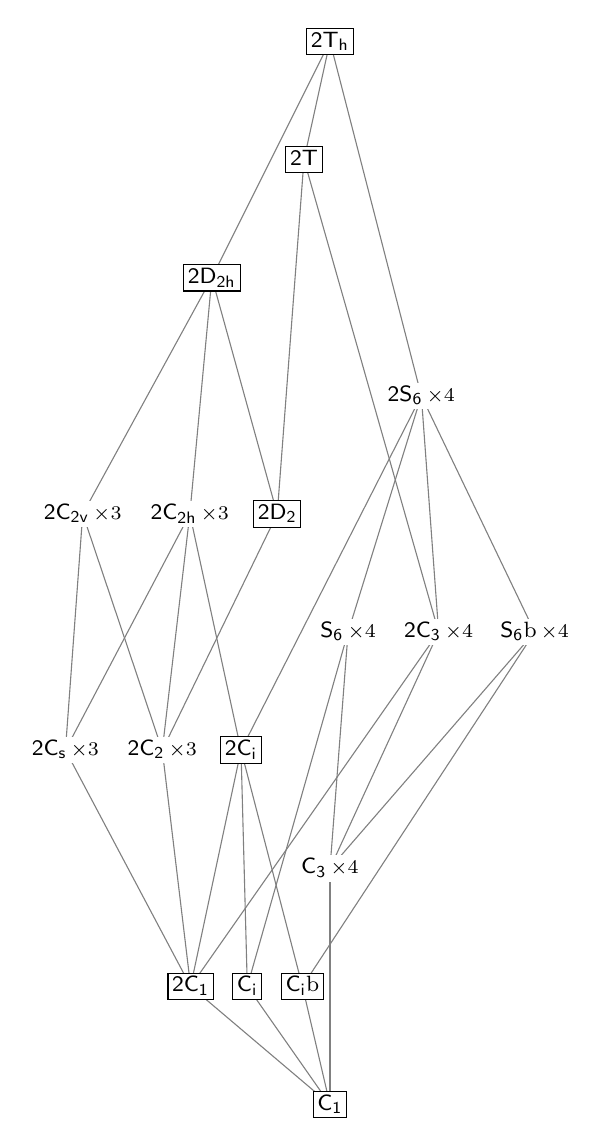
\begin{tikzpicture}[x=1cm, y=1.500cm,
  every node/.style={fill=white, font=\footnotesize, inner xsep=1.5pt, inner ysep=1.2pt, text height=5.6pt, text depth=1.6pt},
  normal/.style={draw, line width=0.4pt}, cover/.style={black!50, line width=0.4pt}]
\draw[cover] (0.00,0) -- (-1.77,1);
\draw[cover] (0.00,0) -- (-1.05,1);
\draw[cover] (0.00,0) -- (-0.35,1);
\draw[cover] (0.00,0) -- (0.00,2);
\draw[cover] (-1.77,1) -- (-2.13,3);
\draw[cover] (-1.77,1) -- (-1.13,3);
\draw[cover] (-1.77,1) -- (-3.36,3);
\draw[cover] (-1.77,1) -- (1.38,4);
\draw[cover] (-1.05,1) -- (-1.13,3);
\draw[cover] (-1.05,1) -- (0.23,4);
\draw[cover] (-0.35,1) -- (-1.13,3);
\draw[cover] (-0.35,1) -- (2.60,4);
\draw[cover] (0.00,2) -- (1.38,4);
\draw[cover] (0.00,2) -- (0.23,4);
\draw[cover] (0.00,2) -- (2.60,4);
\draw[cover] (-2.13,3) -- (-0.67,5);
\draw[cover] (-2.13,3) -- (-1.78,5);
\draw[cover] (-2.13,3) -- (-3.14,5);
\draw[cover] (-1.13,3) -- (-1.78,5);
\draw[cover] (-1.13,3) -- (1.16,6);
\draw[cover] (-3.36,3) -- (-1.78,5);
\draw[cover] (-3.36,3) -- (-3.14,5);
\draw[cover] (1.38,4) -- (1.16,6);
\draw[cover] (1.38,4) -- (-0.33,8);
\draw[cover] (0.23,4) -- (1.16,6);
\draw[cover] (2.60,4) -- (1.16,6);
\draw[cover] (-0.67,5) -- (-1.50,7);
\draw[cover] (-0.67,5) -- (-0.33,8);
\draw[cover] (-1.78,5) -- (-1.50,7);
\draw[cover] (-3.14,5) -- (-1.50,7);
\draw[cover] (1.16,6) -- (0.00,9);
\draw[cover] (-1.50,7) -- (0.00,9);
\draw[cover] (-0.33,8) -- (0.00,9);
\node[normal] (n00) at (0.00,0) {$\grp{C_{1}}$};
\node[normal] (n01) at (-1.77,1) {$\grp{2C_{1}}$};
\node[normal] (n02) at (-1.05,1) {$\grp{C_{i}}$};
\node[normal] (n03) at (-0.35,1) {$\grp{C_{i}}\secondclass$};
\node (n04) at (0.00,2) {$\grp{C_{3}}$\,\nconj{4}};
\node (n05) at (-2.13,3) {$\grp{2C_{2}}$\,\nconj{3}};
\node[normal] (n06) at (-1.13,3) {$\grp{2C_{i}}$};
\node (n07) at (-3.36,3) {$\grp{2C_{s}}$\,\nconj{3}};
\node (n08) at (1.38,4) {$\grp{2C_{3}}$\,\nconj{4}};
\node (n09) at (0.23,4) {$\grp{S_{6}}$\,\nconj{4}};
\node (n10) at (2.60,4) {$\grp{S_{6}}\secondclass$\,\nconj{4}};
\node[normal] (n11) at (-0.67,5) {$\grp{2D_{2}}$};
\node (n12) at (-1.78,5) {$\grp{2C_{2h}}$\,\nconj{3}};
\node (n13) at (-3.14,5) {$\grp{2C_{2v}}$\,\nconj{3}};
\node (n14) at (1.16,6) {$\grp{2S_{6}}$\,\nconj{4}};
\node[normal] (n15) at (-1.50,7) {$\grp{2D_{2h}}$};
\node[normal] (n16) at (-0.33,8) {$\grp{2T}$};
\node[normal] (n17) at (0.00,9) {$\grp{2T_{h}}$};
\end{tikzpicture}
\end{center}
{\small\setlength{\fillwidth}{\textwidth}\addtolength{\fillwidth}{-12\tabcolsep}\setlength{\colwidth}{0pt}\cellmax{$\grp{2C_{2h}}$ $\samecls$ $\grp{2D_{1d}}$}\cellmax{$\grp{2C_{2v}}$ $\samecls$ $\grp{2D_{1h}}$}\cellmax{$\grp{2C_{s}}$ $\samecls$ $\grp{2C_{1h}}$}\cellmax{$\grp{2C_{2}}$ $\samecls$ $\grp{2D_{1}}$}\cellmax{subgrp}\cellmax{$\grp{2D_{2h}}$}\cellmax{$\grp{2C_{1}}$}\cellmax{$\grp{2C_{3}}$}\cellmax{$\grp{2C_{i}}$}\cellmax{$\grp{2D_{2}}$}\cellmax{$\grp{2S_{6}}$}\cellmax{$\grp{2T_{h}}$}\cellmax{$\grp{C_{i}}\secondclass$}\cellmax{$\grp{S_{6}}\secondclass$}\cellmax{$\grp{2T}$}\cellmax{$\grp{C_{1}}$}\cellmax{$\grp{C_{3}}$}\cellmax{$\grp{C_{i}}$}\cellmax{$\grp{S_{6}}$}\addtolength{\fillwidth}{-\colwidth}\setlength{\colwidth}{0pt}\cellmax{order}\cellmax{12}\cellmax{16}\cellmax{24}\cellmax{48}\cellmax{1}\cellmax{2}\cellmax{3}\cellmax{4}\cellmax{6}\cellmax{8}\addtolength{\fillwidth}{-\colwidth}\setlength{\colwidth}{0pt}\cellmax{conjugates}\cellmax{1}\cellmax{3}\cellmax{4}\addtolength{\fillwidth}{-\colwidth}\setlength{\colwidth}{0pt}\cellmax{normal}\cellmax{yes}\cellmax{no}\addtolength{\fillwidth}{-\colwidth}\setlength{\colwidth}{0pt}\cellmax{$\grp{N}_{\hairsp \grp{2T_{h}}}(\grp{H})$}\cellmax{$\grp{2D_{2h}}$}\cellmax{$\grp{2S_{6}}$}\cellmax{$\grp{2T_{h}}$}\addtolength{\fillwidth}{-\colwidth}\setlength{\colwidth}{0pt}\cellmax{$\grp{C}_{\hairsp \grp{2T_{h}}}(\grp{H})$}\cellmax{$\grp{2C_{2h}}$}\cellmax{$\grp{2C_{i}}$}\cellmax{$\grp{2S_{6}}$}\cellmax{$\grp{2T_{h}}$}\addtolength{\fillwidth}{-\colwidth}\setlength{\colwidth}{0pt}\cellmax{$\cls{\barred{E}}$, $\cls{4C_{3}}$, $\cls{4\barred{C}_{3}}$, $\cls{4C_{3}^{2}}$, $\cls{4\barred{C}_{3}^{2}}$, $\cls{i}$, $\cls{\barred{i}}$, $\cls{4S_{6}}$, $\cls{4\barred{S}_{6}}$, $\cls{4S_{6}^{5}}$, $\cls{4\barred{S}_{6}^{5}}$}\cellmax{$\cls{\barred{E}}$, $\cls{4C_{3}}$, $\cls{4\barred{C}_{3}}$, $\cls{4C_{3}^{2}}$, $\cls{4\barred{C}_{3}^{2}}$, $\cls{6C_{2}}$}\cellmax{$\cls{4\barred{C}_{3}}$, $\cls{4\barred{C}_{3}^{2}}$, $\cls{i}$, $\cls{4\barred{S}_{6}}$, $\cls{4\barred{S}_{6}^{5}}$}\cellmax{$\cls{4\barred{C}_{3}}$, $\cls{4\barred{C}_{3}^{2}}$, $\cls{\barred{i}}$, $\cls{4S_{6}}$, $\cls{4S_{6}^{5}}$}\cellmax{$\cls{\barred{E}}$, $\cls{4C_{3}}$, $\cls{4\barred{C}_{3}}$, $\cls{4C_{3}^{2}}$, $\cls{4\barred{C}_{3}^{2}}$}\cellmax{$\cls{\barred{E}}$, $\cls{6C_{2}}$, $\cls{i}$, $\cls{\barred{i}}$, $\cls{6\sigma_{h}}$}\cellmax{$\cls{4\barred{C}_{3}}$, $\cls{4\barred{C}_{3}^{2}}$}\cellmax{$\cls{\barred{E}}$, $\cls{6C_{2}}$, $\cls{6\sigma_{h}}$}\cellmax{$\cls{\barred{E}}$, $\cls{i}$, $\cls{\barred{i}}$}\cellmax{classes}\cellmax{$\cls{\barred{E}}$, $\cls{6C_{2}}$}\cellmax{$\cls{\barred{E}}$, $\cls{6\sigma_{h}}$}\cellmax{---}\cellmax{all}\cellmax{$\cls{\barred{E}}$}\cellmax{$\cls{\barred{i}}$}\cellmax{$\cls{i}$}\fillcap\begin{longtable}{@{}lrrlll>{\RaggedRight\arraybackslash}p{\fillwidth}@{}}\toprule
subgrp & order & conjugates & normal & $\grp{N}_{\hairsp \grp{2T_{h}}}(\grp{H})$ & $\grp{C}_{\hairsp \grp{2T_{h}}}(\grp{H})$ & classes\\\midrule\endhead
\bottomrule\endfoot\endlastfoot
\href{C1.pdf}{$\grp{C_{1}}$} & 1 & 1 & yes & \href{2Th.pdf}{$\grp{2T_{h}}$} & \href{2Th.pdf}{$\grp{2T_{h}}$} & ---\\*
\href{2C1.pdf}{$\grp{2C_{1}}$} & 2 & 1 & yes & \href{2Th.pdf}{$\grp{2T_{h}}$} & \href{2Th.pdf}{$\grp{2T_{h}}$} & $\cls{\barred{E}}$\\
\href{S2.pdf}{$\grp{C_{i}}$} & 2 & 1 & yes & \href{2Th.pdf}{$\grp{2T_{h}}$} & \href{2Th.pdf}{$\grp{2T_{h}}$} & $\cls{i}$\\
\href{S2b.pdf}{$\grp{C_{i}}\secondclass$} & 2 & 1 & yes & \href{2Th.pdf}{$\grp{2T_{h}}$} & \href{2Th.pdf}{$\grp{2T_{h}}$} & $\cls{\barred{i}}$\\
\href{C3.pdf}{$\grp{C_{3}}$} & 3 & 4 & no & \href{2S6.pdf}{$\grp{2S_{6}}$} & \href{2S6.pdf}{$\grp{2S_{6}}$} & $\cls{4\barred{C}_{3}}$, $\cls{4\barred{C}_{3}^{2}}$\\
\href{2C2.pdf}{$\grp{2C_{2}}$} $\samecls$ \href{2D1.pdf}{$\grp{2D_{1}}$} & 4 & 3 & no & \href{2D2h.pdf}{$\grp{2D_{2h}}$} & \href{2C2h.pdf}{$\grp{2C_{2h}}$} & $\cls{\barred{E}}$, $\cls{6C_{2}}$\\
\href{2S2.pdf}{$\grp{2C_{i}}$} & 4 & 1 & yes & \href{2Th.pdf}{$\grp{2T_{h}}$} & \href{2Th.pdf}{$\grp{2T_{h}}$} & $\cls{\barred{E}}$, $\cls{i}$, $\cls{\barred{i}}$\\
\href{2C1v.pdf}{$\grp{2C_{s}}$} $\samecls$ \href{2C1h.pdf}{$\grp{2C_{1h}}$} & 4 & 3 & no & \href{2D2h.pdf}{$\grp{2D_{2h}}$} & \href{2C2h.pdf}{$\grp{2C_{2h}}$} & $\cls{\barred{E}}$, $\cls{6\sigma_{h}}$\\
\href{2C3.pdf}{$\grp{2C_{3}}$} & 6 & 4 & no & \href{2S6.pdf}{$\grp{2S_{6}}$} & \href{2S6.pdf}{$\grp{2S_{6}}$} & $\cls{\barred{E}}$, $\cls{4C_{3}}$, $\cls{4\barred{C}_{3}}$, $\cls{4C_{3}^{2}}$, $\cls{4\barred{C}_{3}^{2}}$\\
\href{S6.pdf}{$\grp{S_{6}}$} & 6 & 4 & no & \href{2S6.pdf}{$\grp{2S_{6}}$} & \href{2S6.pdf}{$\grp{2S_{6}}$} & $\cls{4\barred{C}_{3}}$, $\cls{4\barred{C}_{3}^{2}}$, $\cls{i}$, $\cls{4\barred{S}_{6}}$, $\cls{4\barred{S}_{6}^{5}}$\\
\href{S6b.pdf}{$\grp{S_{6}}\secondclass$} & 6 & 4 & no & \href{2S6.pdf}{$\grp{2S_{6}}$} & \href{2S6.pdf}{$\grp{2S_{6}}$} & $\cls{4\barred{C}_{3}}$, $\cls{4\barred{C}_{3}^{2}}$, $\cls{\barred{i}}$, $\cls{4S_{6}}$, $\cls{4S_{6}^{5}}$\\
\href{2C2h.pdf}{$\grp{2C_{2h}}$} $\samecls$ \href{2D1d.pdf}{$\grp{2D_{1d}}$} & 8 & 3 & no & \href{2D2h.pdf}{$\grp{2D_{2h}}$} & \href{2C2h.pdf}{$\grp{2C_{2h}}$} & $\cls{\barred{E}}$, $\cls{6C_{2}}$, $\cls{i}$, $\cls{\barred{i}}$, $\cls{6\sigma_{h}}$\\
\href{2C2v.pdf}{$\grp{2C_{2v}}$} $\samecls$ \href{2D1h.pdf}{$\grp{2D_{1h}}$} & 8 & 3 & no & \href{2D2h.pdf}{$\grp{2D_{2h}}$} & \href{2S2.pdf}{$\grp{2C_{i}}$} & $\cls{\barred{E}}$, $\cls{6C_{2}}$, $\cls{6\sigma_{h}}$\\
\href{2D2.pdf}{$\grp{2D_{2}}$} & 8 & 1 & yes & \href{2Th.pdf}{$\grp{2T_{h}}$} & \href{2S2.pdf}{$\grp{2C_{i}}$} & $\cls{\barred{E}}$, $\cls{6C_{2}}$\\
\href{2S6.pdf}{$\grp{2S_{6}}$} & 12 & 4 & no & \href{2S6.pdf}{$\grp{2S_{6}}$} & \href{2S6.pdf}{$\grp{2S_{6}}$} & $\cls{\barred{E}}$, $\cls{4C_{3}}$, $\cls{4\barred{C}_{3}}$, $\cls{4C_{3}^{2}}$, $\cls{4\barred{C}_{3}^{2}}$, $\cls{i}$, $\cls{\barred{i}}$, $\cls{4S_{6}}$, $\cls{4\barred{S}_{6}}$, $\cls{4S_{6}^{5}}$, $\cls{4\barred{S}_{6}^{5}}$\\
\href{2D2h.pdf}{$\grp{2D_{2h}}$} & 16 & 1 & yes & \href{2Th.pdf}{$\grp{2T_{h}}$} & \href{2S2.pdf}{$\grp{2C_{i}}$} & $\cls{\barred{E}}$, $\cls{6C_{2}}$, $\cls{i}$, $\cls{\barred{i}}$, $\cls{6\sigma_{h}}$\\
\href{2T.pdf}{$\grp{2T}$} & 24 & 1 & yes & \href{2Th.pdf}{$\grp{2T_{h}}$} & \href{2S2.pdf}{$\grp{2C_{i}}$} & $\cls{\barred{E}}$, $\cls{4C_{3}}$, $\cls{4\barred{C}_{3}}$, $\cls{4C_{3}^{2}}$, $\cls{4\barred{C}_{3}^{2}}$, $\cls{6C_{2}}$\\*
\href{2Th.pdf}{$\grp{2T_{h}}$} & 48 & 1 & yes & \href{2Th.pdf}{$\grp{2T_{h}}$} & \href{2S2.pdf}{$\grp{2C_{i}}$} & all\\
\bottomrule\end{longtable}}
\needspace{103pt}
\section{Descent of symmetry}\label{s:subduction}
Conventions: \href{../../CONVENTIONS.pdf}{CONVENTIONS.pdf}, sections \href{../../../rotation/CONVENTIONS.pdf\#conv.12.2}{12.2}, \href{../../../rotation/CONVENTIONS.pdf\#conv.12.4}{12.4} and \href{../../CONVENTIONS.pdf\#conv.28}{28}.
A column is a class of subgroups $\grp{H}$, in the order of the table of section~\ref{s:subgroups}, by its symbol in the row subgrp as there, with the letter that tells apart classes with the same symbol, which are not conjugate in $\grp{2T_{h}}$; the symbol links to the document of $\grp{H}$. The entry of row $\Gamma$ is $\restr{\Gamma}{\grp{H}}$, the restriction of $\Gamma$ along a monomorphism from the record of $\grp{H}$ onto the subgroup, as a sum of the irreps of $\grp{H}$; the monomorphism identifies the subgroup with its record, and $\grp{H}$ names both. The rows of the vector irreps of a preimage are those of \href{../../../rotation/data/pdf/Th.pdf}{$\grp{T_{h}}$} (\texttt{vector\symbol{95}subduction}); the column of a section is that of its preimage with the spinor irreps renamed (\href{../../CONVENTIONS.pdf}{CONVENTIONS.pdf}, section \href{../../CONVENTIONS.pdf\#conv.27}{27}), which the record does not store. \label{n:group.normalizer.o3}\label{n:group.centralizer.o3}\label{n:element.h}The record of $\grp{H}$ maps onto the subgroup in $\grpindex{\grp{N}}{\grp{C}}$ ways, $h \mapsto g h g^{-1}$ ($h \in \grp{H}$) for the $g \in \grp{Pin^{-}(3)}$ that carry $\grp{H}$ to it, $\grp{N}$ and $\grp{C}$ the normalizer and the centralizer of $\grp{H}$ in $\grp{Pin^{-}(3)}$; the row centralizer of section Names and structure of the document of $\grp{H}$ gives $\grp{C}$ and this index. Two maps related by a conjugation in $\grp{2T_{h}}$ give the same restriction, so the maps fall into $\grpindex{\grp{N}}{\grp{C}}/\grpindex{\grp{N}_{\hairsp \grp{2T_{h}}}}{\grp{C}_{\hairsp \grp{2T_{h}}}}$ classes, $\grp{N}_{\hairsp \grp{2T_{h}}}$ and $\grp{C}_{\hairsp \grp{2T_{h}}}$ the normalizer and the centralizer of the subgroup in $\grp{2T_{h}}$ (the table of section~\ref{s:subgroups}). \label{n:head.setting}A subgroup whose classes give different tables has one column per table, its settings: 1 for the stored monomorphism (\texttt{monomorphism}) and 2, 3, \dots{} for the \texttt{alternative\symbol{95}settings}, each with the images of the generators of $\grp{H}$ (\texttt{setting}). \label{n:head.images}\label{n:element.generator.index}The row images gives, under each setting, each generator of $\grp{H}$ whose image differs between the settings, by the symbol of its class (\href{../../CONVENTIONS.pdf}{CONVENTIONS.pdf}, section \href{../../../rotation/CONVENTIONS.pdf\#conv.5.1}{5.1}), mapped to the class of $\grp{2T_{h}}$ that holds its image; where two generators share a symbol, a superscript number in brackets gives the generator's index in the document of $\grp{H}$. \label{n:irrep.Delta}Each other column under a subgroup is column 1 with each irrep $\Lambda$ of $\grp{H}$ replaced by $\Lambda$ composed with one automorphism of $\grp{H}$ that a conjugation in $\grp{Pin^{-}(3)}$ induces and none in $\grp{2T_{h}}$ does (\href{../../CONVENTIONS.pdf}{CONVENTIONS.pdf}, section \href{../../../rotation/CONVENTIONS.pdf\#conv.12.1}{12.1}).
{\small\begin{longtable}{@{}lccccccc@{}}\toprule
subgrp & \href{2C1.pdf}{$\grp{2C_{1}}$} & \href{S2.pdf}{$\grp{C_{i}}$} & \href{S2b.pdf}{$\grp{C_{i}}\secondclass$} & \href{C3.pdf}{$\grp{C_{3}}$} & \href{2C2.pdf}{$\grp{2C_{2}}$} & \href{2S2.pdf}{$\grp{2C_{i}}$} & \href{2C1v.pdf}{$\grp{2C_{s}}$}\\\midrule\endhead
\bottomrule\endfoot\endlastfoot
$\irr{a}_{\ptag{g}}$ & $\irr{a}$ & $\irr{a}_{\ptag{g}}$ & $\irr{a}_{\ptag{g}}$ & $\irr{a}$ & $\irr{a}$ & $\irr{a}_{\ptag{g}}$ & $\irr{a}'$\\*
$\conjpair{1}\irr{e}_{\ptag{g}}$ & $\irr{a}$ & $\irr{a}_{\ptag{g}}$ & $\irr{a}_{\ptag{g}}$ & $\conjpair{1}\irr{e}$ & $\irr{a}$ & $\irr{a}_{\ptag{g}}$ & $\irr{a}'$\\
$\conjpair{2}\irr{e}_{\ptag{g}}$ & $\irr{a}$ & $\irr{a}_{\ptag{g}}$ & $\irr{a}_{\ptag{g}}$ & $\conjpair{2}\irr{e}$ & $\irr{a}$ & $\irr{a}_{\ptag{g}}$ & $\irr{a}'$\\
$\irr{t}_{\ptag{g}}$ & $3\,\irr{a}$ & $3\,\irr{a}_{\ptag{g}}$ & $3\,\irr{a}_{\ptag{g}}$ & $\irr{a}\oplus \conjpair{1}\irr{e}\oplus \conjpair{2}\irr{e}$ & $\irr{a}\oplus 2\,\irr{b}$ & $3\,\irr{a}_{\ptag{g}}$ & $\irr{a}'\oplus 2\,\irr{a}''$\\
$\irr{a}_{\ptag{u}}$ & $\irr{a}$ & $\irr{a}_{\ptag{u}}$ & $\irr{a}_{\ptag{u}}$ & $\irr{a}$ & $\irr{a}$ & $\irr{a}_{\ptag{u}}$ & $\irr{a}''$\\
$\conjpair{1}\irr{e}_{\ptag{u}}$ & $\irr{a}$ & $\irr{a}_{\ptag{u}}$ & $\irr{a}_{\ptag{u}}$ & $\conjpair{1}\irr{e}$ & $\irr{a}$ & $\irr{a}_{\ptag{u}}$ & $\irr{a}''$\\
$\conjpair{2}\irr{e}_{\ptag{u}}$ & $\irr{a}$ & $\irr{a}_{\ptag{u}}$ & $\irr{a}_{\ptag{u}}$ & $\conjpair{2}\irr{e}$ & $\irr{a}$ & $\irr{a}_{\ptag{u}}$ & $\irr{a}''$\\
$\irr{t}_{\ptag{u}}$ & $3\,\irr{a}$ & $3\,\irr{a}_{\ptag{u}}$ & $3\,\irr{a}_{\ptag{u}}$ & $\irr{a}\oplus \conjpair{1}\irr{e}\oplus \conjpair{2}\irr{e}$ & $\irr{a}\oplus 2\,\irr{b}$ & $3\,\irr{a}_{\ptag{u}}$ & $2\,\irr{a}'\oplus \irr{a}''$\\
$\irr{e}_{1/2,\ptag{g}}$ & $2\,\irr{a}_{1/2}$ & $2\,\irr{a}_{\ptag{g}}$ & $2\,\irr{a}_{\ptag{u}}$ & $\conjpair{2}\irr{e}\oplus \conjpair{1}\irr{e}$ & $\conjpair{1}\irr{e}_{1/2}\oplus \conjpair{2}\irr{e}_{1/2}$ & $2\,\irr{a}_{1/2,\ptag{g}}$ & $\conjpair{1}\irr{e}_{1/2}\oplus \conjpair{2}\irr{e}_{1/2}$\\
$\conjpair{1}\irr{g}_{3/2,\ptag{g}}$ & $2\,\irr{a}_{1/2}$ & $2\,\irr{a}_{\ptag{g}}$ & $2\,\irr{a}_{\ptag{u}}$ & $\irr{a}\oplus \conjpair{2}\irr{e}$ & $\conjpair{1}\irr{e}_{1/2}\oplus \conjpair{2}\irr{e}_{1/2}$ & $2\,\irr{a}_{1/2,\ptag{g}}$ & $\conjpair{1}\irr{e}_{1/2}\oplus \conjpair{2}\irr{e}_{1/2}$\\
$\conjpair{2}\irr{g}_{3/2,\ptag{g}}$ & $2\,\irr{a}_{1/2}$ & $2\,\irr{a}_{\ptag{g}}$ & $2\,\irr{a}_{\ptag{u}}$ & $\irr{a}\oplus \conjpair{1}\irr{e}$ & $\conjpair{1}\irr{e}_{1/2}\oplus \conjpair{2}\irr{e}_{1/2}$ & $2\,\irr{a}_{1/2,\ptag{g}}$ & $\conjpair{1}\irr{e}_{1/2}\oplus \conjpair{2}\irr{e}_{1/2}$\\
$\irr{e}_{1/2,\ptag{u}}$ & $2\,\irr{a}_{1/2}$ & $2\,\irr{a}_{\ptag{u}}$ & $2\,\irr{a}_{\ptag{g}}$ & $\conjpair{2}\irr{e}\oplus \conjpair{1}\irr{e}$ & $\conjpair{1}\irr{e}_{1/2}\oplus \conjpair{2}\irr{e}_{1/2}$ & $2\,\irr{a}_{1/2,\ptag{u}}$ & $\conjpair{1}\irr{e}_{1/2}\oplus \conjpair{2}\irr{e}_{1/2}$\\
$\conjpair{1}\irr{g}_{3/2,\ptag{u}}$ & $2\,\irr{a}_{1/2}$ & $2\,\irr{a}_{\ptag{u}}$ & $2\,\irr{a}_{\ptag{g}}$ & $\irr{a}\oplus \conjpair{2}\irr{e}$ & $\conjpair{1}\irr{e}_{1/2}\oplus \conjpair{2}\irr{e}_{1/2}$ & $2\,\irr{a}_{1/2,\ptag{u}}$ & $\conjpair{1}\irr{e}_{1/2}\oplus \conjpair{2}\irr{e}_{1/2}$\\*
$\conjpair{2}\irr{g}_{3/2,\ptag{u}}$ & $2\,\irr{a}_{1/2}$ & $2\,\irr{a}_{\ptag{u}}$ & $2\,\irr{a}_{\ptag{g}}$ & $\irr{a}\oplus \conjpair{1}\irr{e}$ & $\conjpair{1}\irr{e}_{1/2}\oplus \conjpair{2}\irr{e}_{1/2}$ & $2\,\irr{a}_{1/2,\ptag{u}}$ & $\conjpair{1}\irr{e}_{1/2}\oplus \conjpair{2}\irr{e}_{1/2}$\\
\bottomrule\end{longtable}}
{\small\begin{longtable}{@{}lccccc@{}}\toprule
subgrp & \multicolumn{2}{c}{\href{2C3.pdf}{$\grp{2C_{3}}$}} & \href{S6.pdf}{$\grp{S_{6}}$} & \href{S6b.pdf}{$\grp{S_{6}}\secondclass$} & \href{2C2h.pdf}{$\grp{2C_{2h}}$}\\\cmidrule(lr){2-3}
setting & 1 & 2 &  &  & \\
images & {\scriptsize $\cls{C_{3}} \mapsto \cls{4C_{3}}$} & {\scriptsize $\cls{C_{3}} \mapsto \cls{4C_{3}^{2}}$} &  &  & \\\midrule\endhead
\bottomrule\endfoot\endlastfoot
$\irr{a}_{\ptag{g}}$ & $\irr{a}$ & $\irr{a}$ & $\irr{a}_{\ptag{g}}$ & $\irr{a}_{\ptag{g}}$ & $\irr{a}_{\ptag{g}}$\\*
$\conjpair{1}\irr{e}_{\ptag{g}}$ & $\conjpair{1}\irr{e}$ & $\conjpair{2}\irr{e}$ & $\conjpair{1}\irr{e}_{\ptag{g}}$ & $\conjpair{1}\irr{e}_{\ptag{g}}$ & $\irr{a}_{\ptag{g}}$\\
$\conjpair{2}\irr{e}_{\ptag{g}}$ & $\conjpair{2}\irr{e}$ & $\conjpair{1}\irr{e}$ & $\conjpair{2}\irr{e}_{\ptag{g}}$ & $\conjpair{2}\irr{e}_{\ptag{g}}$ & $\irr{a}_{\ptag{g}}$\\
$\irr{t}_{\ptag{g}}$ & $\irr{a}\oplus \conjpair{1}\irr{e}\oplus \conjpair{2}\irr{e}$ & $\irr{a}\oplus \conjpair{1}\irr{e}\oplus \conjpair{2}\irr{e}$ & $\irr{a}_{\ptag{g}}\oplus \conjpair{1}\irr{e}_{\ptag{g}}\oplus \conjpair{2}\irr{e}_{\ptag{g}}$ & $\irr{a}_{\ptag{g}}\oplus \conjpair{1}\irr{e}_{\ptag{g}}\oplus \conjpair{2}\irr{e}_{\ptag{g}}$ & $\irr{a}_{\ptag{g}}\oplus 2\,\irr{b}_{\ptag{g}}$\\
$\irr{a}_{\ptag{u}}$ & $\irr{a}$ & $\irr{a}$ & $\irr{a}_{\ptag{u}}$ & $\irr{a}_{\ptag{u}}$ & $\irr{a}_{\ptag{u}}$\\
$\conjpair{1}\irr{e}_{\ptag{u}}$ & $\conjpair{1}\irr{e}$ & $\conjpair{2}\irr{e}$ & $\conjpair{1}\irr{e}_{\ptag{u}}$ & $\conjpair{1}\irr{e}_{\ptag{u}}$ & $\irr{a}_{\ptag{u}}$\\
$\conjpair{2}\irr{e}_{\ptag{u}}$ & $\conjpair{2}\irr{e}$ & $\conjpair{1}\irr{e}$ & $\conjpair{2}\irr{e}_{\ptag{u}}$ & $\conjpair{2}\irr{e}_{\ptag{u}}$ & $\irr{a}_{\ptag{u}}$\\
$\irr{t}_{\ptag{u}}$ & $\irr{a}\oplus \conjpair{1}\irr{e}\oplus \conjpair{2}\irr{e}$ & $\irr{a}\oplus \conjpair{1}\irr{e}\oplus \conjpair{2}\irr{e}$ & $\irr{a}_{\ptag{u}}\oplus \conjpair{1}\irr{e}_{\ptag{u}}\oplus \conjpair{2}\irr{e}_{\ptag{u}}$ & $\irr{a}_{\ptag{u}}\oplus \conjpair{1}\irr{e}_{\ptag{u}}\oplus \conjpair{2}\irr{e}_{\ptag{u}}$ & $\irr{a}_{\ptag{u}}\oplus 2\,\irr{b}_{\ptag{u}}$\\
$\irr{e}_{1/2,\ptag{g}}$ & $\conjpair{1}\irr{e}_{1/2}\oplus \conjpair{2}\irr{e}_{1/2}$ & $\conjpair{1}\irr{e}_{1/2}\oplus \conjpair{2}\irr{e}_{1/2}$ & $\conjpair{2}\irr{e}_{\ptag{g}}\oplus \conjpair{1}\irr{e}_{\ptag{g}}$ & $\conjpair{2}\irr{e}_{\ptag{u}}\oplus \conjpair{1}\irr{e}_{\ptag{u}}$ & $\conjpair{1}\irr{e}_{1/2,\ptag{g}}\oplus \conjpair{2}\irr{e}_{1/2,\ptag{g}}$\\
$\conjpair{1}\irr{g}_{3/2,\ptag{g}}$ & $\irr{a}_{3/2}\oplus \conjpair{1}\irr{e}_{1/2}$ & $\irr{a}_{3/2}\oplus \conjpair{2}\irr{e}_{1/2}$ & $\irr{a}_{\ptag{g}}\oplus \conjpair{2}\irr{e}_{\ptag{g}}$ & $\irr{a}_{\ptag{u}}\oplus \conjpair{2}\irr{e}_{\ptag{u}}$ & $\conjpair{1}\irr{e}_{1/2,\ptag{g}}\oplus \conjpair{2}\irr{e}_{1/2,\ptag{g}}$\\
$\conjpair{2}\irr{g}_{3/2,\ptag{g}}$ & $\irr{a}_{3/2}\oplus \conjpair{2}\irr{e}_{1/2}$ & $\irr{a}_{3/2}\oplus \conjpair{1}\irr{e}_{1/2}$ & $\irr{a}_{\ptag{g}}\oplus \conjpair{1}\irr{e}_{\ptag{g}}$ & $\irr{a}_{\ptag{u}}\oplus \conjpair{1}\irr{e}_{\ptag{u}}$ & $\conjpair{1}\irr{e}_{1/2,\ptag{g}}\oplus \conjpair{2}\irr{e}_{1/2,\ptag{g}}$\\
$\irr{e}_{1/2,\ptag{u}}$ & $\conjpair{1}\irr{e}_{1/2}\oplus \conjpair{2}\irr{e}_{1/2}$ & $\conjpair{1}\irr{e}_{1/2}\oplus \conjpair{2}\irr{e}_{1/2}$ & $\conjpair{2}\irr{e}_{\ptag{u}}\oplus \conjpair{1}\irr{e}_{\ptag{u}}$ & $\conjpair{2}\irr{e}_{\ptag{g}}\oplus \conjpair{1}\irr{e}_{\ptag{g}}$ & $\conjpair{1}\irr{e}_{1/2,\ptag{u}}\oplus \conjpair{2}\irr{e}_{1/2,\ptag{u}}$\\
$\conjpair{1}\irr{g}_{3/2,\ptag{u}}$ & $\irr{a}_{3/2}\oplus \conjpair{1}\irr{e}_{1/2}$ & $\irr{a}_{3/2}\oplus \conjpair{2}\irr{e}_{1/2}$ & $\irr{a}_{\ptag{u}}\oplus \conjpair{2}\irr{e}_{\ptag{u}}$ & $\irr{a}_{\ptag{g}}\oplus \conjpair{2}\irr{e}_{\ptag{g}}$ & $\conjpair{1}\irr{e}_{1/2,\ptag{u}}\oplus \conjpair{2}\irr{e}_{1/2,\ptag{u}}$\\*
$\conjpair{2}\irr{g}_{3/2,\ptag{u}}$ & $\irr{a}_{3/2}\oplus \conjpair{2}\irr{e}_{1/2}$ & $\irr{a}_{3/2}\oplus \conjpair{1}\irr{e}_{1/2}$ & $\irr{a}_{\ptag{u}}\oplus \conjpair{1}\irr{e}_{\ptag{u}}$ & $\irr{a}_{\ptag{g}}\oplus \conjpair{1}\irr{e}_{\ptag{g}}$ & $\conjpair{1}\irr{e}_{1/2,\ptag{u}}\oplus \conjpair{2}\irr{e}_{1/2,\ptag{u}}$\\
\bottomrule\end{longtable}}
{\small\begin{longtable}{@{}lccccc@{}}\toprule
subgrp & \href{2C2v.pdf}{$\grp{2C_{2v}}$} & \href{2D2.pdf}{$\grp{2D_{2}}$} & \multicolumn{2}{c}{\href{2S6.pdf}{$\grp{2S_{6}}$}} & \href{2D2h.pdf}{$\grp{2D_{2h}}$}\\\cmidrule(lr){4-5}
setting &  &  & 1 & 2 & \\
images &  &  & {\scriptsize $\cls{C_{3}} \mapsto \cls{4C_{3}}$} & {\scriptsize $\cls{C_{3}} \mapsto \cls{4C_{3}^{2}}$} & \\\midrule\endhead
\bottomrule\endfoot\endlastfoot
$\irr{a}_{\ptag{g}}$ & $\irr{a}_{1}$ & $\irr{a}$ & $\irr{a}_{\ptag{g}}$ & $\irr{a}_{\ptag{g}}$ & $\irr{a}_{\ptag{g}}$\\*
$\conjpair{1}\irr{e}_{\ptag{g}}$ & $\irr{a}_{1}$ & $\irr{a}$ & $\conjpair{1}\irr{e}_{\ptag{g}}$ & $\conjpair{2}\irr{e}_{\ptag{g}}$ & $\irr{a}_{\ptag{g}}$\\
$\conjpair{2}\irr{e}_{\ptag{g}}$ & $\irr{a}_{1}$ & $\irr{a}$ & $\conjpair{2}\irr{e}_{\ptag{g}}$ & $\conjpair{1}\irr{e}_{\ptag{g}}$ & $\irr{a}_{\ptag{g}}$\\
$\irr{t}_{\ptag{g}}$ & $\irr{a}_{2}\oplus \irr{b}_{1}\oplus \irr{b}_{2}$ & $\irr{b}_{1}\oplus \irr{b}_{2}\oplus \irr{b}_{3}$ & $\irr{a}_{\ptag{g}}\oplus \conjpair{1}\irr{e}_{\ptag{g}}\oplus \conjpair{2}\irr{e}_{\ptag{g}}$ & $\irr{a}_{\ptag{g}}\oplus \conjpair{1}\irr{e}_{\ptag{g}}\oplus \conjpair{2}\irr{e}_{\ptag{g}}$ & $\irr{b}_{1\ptag{g}}\oplus \irr{b}_{2\ptag{g}}\oplus \irr{b}_{3\ptag{g}}$\\
$\irr{a}_{\ptag{u}}$ & $\irr{a}_{2}$ & $\irr{a}$ & $\irr{a}_{\ptag{u}}$ & $\irr{a}_{\ptag{u}}$ & $\irr{a}_{\ptag{u}}$\\
$\conjpair{1}\irr{e}_{\ptag{u}}$ & $\irr{a}_{2}$ & $\irr{a}$ & $\conjpair{1}\irr{e}_{\ptag{u}}$ & $\conjpair{2}\irr{e}_{\ptag{u}}$ & $\irr{a}_{\ptag{u}}$\\
$\conjpair{2}\irr{e}_{\ptag{u}}$ & $\irr{a}_{2}$ & $\irr{a}$ & $\conjpair{2}\irr{e}_{\ptag{u}}$ & $\conjpair{1}\irr{e}_{\ptag{u}}$ & $\irr{a}_{\ptag{u}}$\\
$\irr{t}_{\ptag{u}}$ & $\irr{a}_{1}\oplus \irr{b}_{1}\oplus \irr{b}_{2}$ & $\irr{b}_{1}\oplus \irr{b}_{2}\oplus \irr{b}_{3}$ & $\irr{a}_{\ptag{u}}\oplus \conjpair{1}\irr{e}_{\ptag{u}}\oplus \conjpair{2}\irr{e}_{\ptag{u}}$ & $\irr{a}_{\ptag{u}}\oplus \conjpair{1}\irr{e}_{\ptag{u}}\oplus \conjpair{2}\irr{e}_{\ptag{u}}$ & $\irr{b}_{1\ptag{u}}\oplus \irr{b}_{2\ptag{u}}\oplus \irr{b}_{3\ptag{u}}$\\
$\irr{e}_{1/2,\ptag{g}}$ & $\irr{e}_{1/2}$ & $\irr{e}_{1/2}$ & $\conjpair{1}\irr{e}_{1/2,\ptag{g}}\oplus \conjpair{2}\irr{e}_{1/2,\ptag{g}}$ & $\conjpair{1}\irr{e}_{1/2,\ptag{g}}\oplus \conjpair{2}\irr{e}_{1/2,\ptag{g}}$ & $\irr{e}_{1/2,\ptag{g}}$\\
$\conjpair{1}\irr{g}_{3/2,\ptag{g}}$ & $\irr{e}_{1/2}$ & $\irr{e}_{1/2}$ & $\irr{a}_{3/2,\ptag{g}}\oplus \conjpair{1}\irr{e}_{1/2,\ptag{g}}$ & $\irr{a}_{3/2,\ptag{g}}\oplus \conjpair{2}\irr{e}_{1/2,\ptag{g}}$ & $\irr{e}_{1/2,\ptag{g}}$\\
$\conjpair{2}\irr{g}_{3/2,\ptag{g}}$ & $\irr{e}_{1/2}$ & $\irr{e}_{1/2}$ & $\irr{a}_{3/2,\ptag{g}}\oplus \conjpair{2}\irr{e}_{1/2,\ptag{g}}$ & $\irr{a}_{3/2,\ptag{g}}\oplus \conjpair{1}\irr{e}_{1/2,\ptag{g}}$ & $\irr{e}_{1/2,\ptag{g}}$\\
$\irr{e}_{1/2,\ptag{u}}$ & $\irr{e}_{1/2}$ & $\irr{e}_{1/2}$ & $\conjpair{1}\irr{e}_{1/2,\ptag{u}}\oplus \conjpair{2}\irr{e}_{1/2,\ptag{u}}$ & $\conjpair{1}\irr{e}_{1/2,\ptag{u}}\oplus \conjpair{2}\irr{e}_{1/2,\ptag{u}}$ & $\irr{e}_{1/2,\ptag{u}}$\\
$\conjpair{1}\irr{g}_{3/2,\ptag{u}}$ & $\irr{e}_{1/2}$ & $\irr{e}_{1/2}$ & $\irr{a}_{3/2,\ptag{u}}\oplus \conjpair{1}\irr{e}_{1/2,\ptag{u}}$ & $\irr{a}_{3/2,\ptag{u}}\oplus \conjpair{2}\irr{e}_{1/2,\ptag{u}}$ & $\irr{e}_{1/2,\ptag{u}}$\\*
$\conjpair{2}\irr{g}_{3/2,\ptag{u}}$ & $\irr{e}_{1/2}$ & $\irr{e}_{1/2}$ & $\irr{a}_{3/2,\ptag{u}}\oplus \conjpair{2}\irr{e}_{1/2,\ptag{u}}$ & $\irr{a}_{3/2,\ptag{u}}\oplus \conjpair{1}\irr{e}_{1/2,\ptag{u}}$ & $\irr{e}_{1/2,\ptag{u}}$\\
\bottomrule\end{longtable}}
{\small\begin{longtable}{@{}lcc@{}}\toprule
subgrp & \multicolumn{2}{c}{\href{2T.pdf}{$\grp{2T}$}}\\\cmidrule(lr){2-3}
setting & 1 & 2\\
images & {\scriptsize\begin{tabular}[t]{@{}c@{}}$\cls{\genidx{C_{3}}{2}} \mapsto \cls{4C_{3}}$\\$\cls{\genidx{C_{3}}{4}} \mapsto \cls{4C_{3}}$\end{tabular}} & {\scriptsize\begin{tabular}[t]{@{}c@{}}$\cls{\genidx{C_{3}}{2}} \mapsto \cls{4C_{3}^{2}}$\\$\cls{\genidx{C_{3}}{4}} \mapsto \cls{4C_{3}^{2}}$\end{tabular}}\\\midrule\endhead
\bottomrule\endfoot\endlastfoot
$\irr{a}_{\ptag{g}}$ & $\irr{a}$ & $\irr{a}$\\*
$\conjpair{1}\irr{e}_{\ptag{g}}$ & $\conjpair{1}\irr{e}$ & $\conjpair{2}\irr{e}$\\
$\conjpair{2}\irr{e}_{\ptag{g}}$ & $\conjpair{2}\irr{e}$ & $\conjpair{1}\irr{e}$\\
$\irr{t}_{\ptag{g}}$ & $\irr{t}$ & $\irr{t}$\\
$\irr{a}_{\ptag{u}}$ & $\irr{a}$ & $\irr{a}$\\
$\conjpair{1}\irr{e}_{\ptag{u}}$ & $\conjpair{1}\irr{e}$ & $\conjpair{2}\irr{e}$\\
$\conjpair{2}\irr{e}_{\ptag{u}}$ & $\conjpair{2}\irr{e}$ & $\conjpair{1}\irr{e}$\\
$\irr{t}_{\ptag{u}}$ & $\irr{t}$ & $\irr{t}$\\
$\irr{e}_{1/2,\ptag{g}}$ & $\irr{e}_{1/2}$ & $\irr{e}_{1/2}$\\
$\conjpair{1}\irr{g}_{3/2,\ptag{g}}$ & $\conjpair{1}\irr{g}_{3/2}$ & $\conjpair{2}\irr{g}_{3/2}$\\
$\conjpair{2}\irr{g}_{3/2,\ptag{g}}$ & $\conjpair{2}\irr{g}_{3/2}$ & $\conjpair{1}\irr{g}_{3/2}$\\
$\irr{e}_{1/2,\ptag{u}}$ & $\irr{e}_{1/2}$ & $\irr{e}_{1/2}$\\
$\conjpair{1}\irr{g}_{3/2,\ptag{u}}$ & $\conjpair{1}\irr{g}_{3/2}$ & $\conjpair{2}\irr{g}_{3/2}$\\*
$\conjpair{2}\irr{g}_{3/2,\ptag{u}}$ & $\conjpair{2}\irr{g}_{3/2}$ & $\conjpair{1}\irr{g}_{3/2}$\\
\bottomrule\end{longtable}}
Read down a column, a table gives induction (Frobenius reciprocity): $\Gamma$ occurs in $\Ind{\grp{H}}{\grp{2T_{h}}} \Lambda$ as often as $\Lambda$ occurs in the entry of row $\Gamma$. The JSON gives, for every entry of a spinor irrep, the unitary matrix that carries $\restr{\Gamma}{\grp{H}}$ into the direct sum of the matrices of $\grp{H}$ (\texttt{subduction[].blocks}), and for every class the left coset representatives of $\grp{H}$ (\texttt{transversal}), from which \href{../../CONVENTIONS.pdf}{CONVENTIONS.pdf}, section \href{../../../rotation/CONVENTIONS.pdf\#conv.12.4}{12.4}, builds $\Ind{\grp{H}}{\grp{2T_{h}}} \Lambda$ and its intertwiners.
\needspace{190pt}
\partbox{Angular momentum}
\section{Subduction from \texorpdfstring{$\grp{Pin^{-}(3)}$}{Pin\unichar{8315}(3)}}\label{s:subduction_parent}
Conventions: \href{../../CONVENTIONS.pdf}{CONVENTIONS.pdf}, sections \href{../../../rotation/CONVENTIONS.pdf\#conv.11}{11} and \href{../../CONVENTIONS.pdf\#conv.25.1}{25.1}.
\leavevmode\label{n:index.J}\label{n:index.parity}\label{n:irrep.o3}\label{n:function.character.parent}\label{n:function.multiplicity}$\irrJp{J}{p}$ is the irrep of $\grp{Pin^{-}(3)}$ of angular momentum $J$ ($J = 0, \nicefrac{1}{2}, 1, \dots$) and parity $p = \pm 1$, on which $(U, \varepsilon)$ acts as $\varepsilon^{[p = -1]}$ times $U$ acting on the kets of angular momentum $J$; $\elt{\barred{E}}$ acts as $(-1)^{2J}$. An element whose $\grp{SU(2)}$ part is $\lift{R}_{\vv}(\omega)$ (section~\ref{s:elements}) has the character
\begin{equation}\label{e:chi}\chi^{(J,p)}(g) = p^{\iverson{\det g = -1}}\sum_{m=-J}^{J} \expe^{\iunit m\omega},\end{equation}
and $b_\Gamma(J, p)$ is the multiplicity of $\Gamma$ in
\begin{equation}\label{e:parent}\restr{\irrJp{J}{p}}{\grp{2T_{h}}}.\end{equation}
\leavevmode\label{n:index.increment}At integer $J$ only the vector irreps occur, and $b_\Gamma(J, p)$ is the multiplicity of the subduction from $\grp{O(3)}$ in \href{../../../rotation/data/pdf/Th.pdf}{$\grp{T_{h}}$} (\texttt{integer\symbol{95}J}). At half-integer $J$ only the spinor irreps occur: each table gives $b_\Gamma(J, p)$ for $2J \le 41$, and $b_\Gamma(J + 3, p) = b_\Gamma(J, p) + \Delta_\Gamma$ for every $J$ of the table, $\Delta_\Gamma$ its last row. A table leaves out the irreps whose multiplicity is 0 for every $J$.
\leavevmode\label{n:operator.determinant.character}The determinant exchanges the parities: $\irrJp{J}{-1} = \irrJp{J}{+1} \irrprod \det$, so that $b_\Gamma(J, -1) = b_{\Gamma \irrprod \det_{\grp{2T_{h}}}}(J, +1)$.
\needspace{182pt}
\paragraph{Half-integer $J$, $p = +1$.}
{\small\begin{longtable}{@{}rrrr@{\hspace{18pt}}rrrr@{\hspace{18pt}}rrrr@{}}\toprule
$J$ & $\irr{e}_{1/2,\ptag{g}}$ & $\conjpair{1}\irr{g}_{3/2,\ptag{g}}$ & $\conjpair{2}\irr{g}_{3/2,\ptag{g}}$ & $J$ & $\irr{e}_{1/2,\ptag{g}}$ & $\conjpair{1}\irr{g}_{3/2,\ptag{g}}$ & $\conjpair{2}\irr{g}_{3/2,\ptag{g}}$ & $J$ & $\irr{e}_{1/2,\ptag{g}}$ & $\conjpair{1}\irr{g}_{3/2,\ptag{g}}$ & $\conjpair{2}\irr{g}_{3/2,\ptag{g}}$\\\midrule\endhead
\bottomrule\endfoot\endlastfoot
$\nicefrac{1}{2}$ & 1 & 0 & 0 & $\nicefrac{17}{2}$ & 3 & 3 & 3 & $\nicefrac{33}{2}$ & 5 & 6 & 6\\*
$\nicefrac{3}{2}$ & 0 & 1 & 1 & $\nicefrac{19}{2}$ & 4 & 3 & 3 & $\nicefrac{35}{2}$ & 6 & 6 & 6\\*
$\nicefrac{5}{2}$ & 1 & 1 & 1 & $\nicefrac{21}{2}$ & 3 & 4 & 4 & $\nicefrac{37}{2}$ & 7 & 6 & 6\\*
$\nicefrac{7}{2}$ & 2 & 1 & 1 & $\nicefrac{23}{2}$ & 4 & 4 & 4 & $\nicefrac{39}{2}$ & 6 & 7 & 7\\*
$\nicefrac{9}{2}$ & 1 & 2 & 2 & $\nicefrac{25}{2}$ & 5 & 4 & 4 & $\nicefrac{41}{2}$ & 7 & 7 & 7\\*\noalign{\vskip 1.5pt}\multispan{4} & \multispan{4} & \multispan{4}\leaders\hrule height\cmidrulewidth\hfill\kern0pt\\*\noalign{\vskip 1.5pt}
$\nicefrac{11}{2}$ & 2 & 2 & 2 & $\nicefrac{27}{2}$ & 4 & 5 & 5 & $\Delta_\Gamma$ & 1 & 1 & 1\\*
$\nicefrac{13}{2}$ & 3 & 2 & 2 & $\nicefrac{29}{2}$ & 5 & 5 & 5 &  &  &  & \\*
$\nicefrac{15}{2}$ & 2 & 3 & 3 & $\nicefrac{31}{2}$ & 6 & 5 & 5 &  &  &  & \\
\bottomrule\end{longtable}}
\needspace{182pt}
\paragraph{Half-integer $J$, $p = -1$.}
{\small\begin{longtable}{@{}rrrr@{\hspace{18pt}}rrrr@{\hspace{18pt}}rrrr@{}}\toprule
$J$ & $\irr{e}_{1/2,\ptag{u}}$ & $\conjpair{1}\irr{g}_{3/2,\ptag{u}}$ & $\conjpair{2}\irr{g}_{3/2,\ptag{u}}$ & $J$ & $\irr{e}_{1/2,\ptag{u}}$ & $\conjpair{1}\irr{g}_{3/2,\ptag{u}}$ & $\conjpair{2}\irr{g}_{3/2,\ptag{u}}$ & $J$ & $\irr{e}_{1/2,\ptag{u}}$ & $\conjpair{1}\irr{g}_{3/2,\ptag{u}}$ & $\conjpair{2}\irr{g}_{3/2,\ptag{u}}$\\\midrule\endhead
\bottomrule\endfoot\endlastfoot
$\nicefrac{1}{2}$ & 1 & 0 & 0 & $\nicefrac{17}{2}$ & 3 & 3 & 3 & $\nicefrac{33}{2}$ & 5 & 6 & 6\\*
$\nicefrac{3}{2}$ & 0 & 1 & 1 & $\nicefrac{19}{2}$ & 4 & 3 & 3 & $\nicefrac{35}{2}$ & 6 & 6 & 6\\*
$\nicefrac{5}{2}$ & 1 & 1 & 1 & $\nicefrac{21}{2}$ & 3 & 4 & 4 & $\nicefrac{37}{2}$ & 7 & 6 & 6\\*
$\nicefrac{7}{2}$ & 2 & 1 & 1 & $\nicefrac{23}{2}$ & 4 & 4 & 4 & $\nicefrac{39}{2}$ & 6 & 7 & 7\\*
$\nicefrac{9}{2}$ & 1 & 2 & 2 & $\nicefrac{25}{2}$ & 5 & 4 & 4 & $\nicefrac{41}{2}$ & 7 & 7 & 7\\*\noalign{\vskip 1.5pt}\multispan{4} & \multispan{4} & \multispan{4}\leaders\hrule height\cmidrulewidth\hfill\kern0pt\\*\noalign{\vskip 1.5pt}
$\nicefrac{11}{2}$ & 2 & 2 & 2 & $\nicefrac{27}{2}$ & 4 & 5 & 5 & $\Delta_\Gamma$ & 1 & 1 & 1\\*
$\nicefrac{13}{2}$ & 3 & 2 & 2 & $\nicefrac{29}{2}$ & 5 & 5 & 5 &  &  &  & \\*
$\nicefrac{15}{2}$ & 2 & 3 & 3 & $\nicefrac{31}{2}$ & 6 & 5 & 5 &  &  &  & \\
\bottomrule\end{longtable}}
\needspace{110pt}
\section{Multiplicities and allowed \texorpdfstring{$m$}{m}}\label{s:multiplicities}
Conventions: \href{../../CONVENTIONS.pdf}{CONVENTIONS.pdf}, sections \href{../../../rotation/CONVENTIONS.pdf\#conv.14}{14} and \href{../../CONVENTIONS.pdf\#conv.26}{26}.
\leavevmode\label{n:function.generating}\label{n:index.generating.variable}\label{n:function.generating.numerator}$b_\Gamma(J)$ is the number of blocks of $\Gamma$ at $J$, with the generating function
\begin{equation}\label{e:gf}H_\Gamma(t) = \sum_{J\ge1/2} b_\Gamma(J)\,t^{2J} = P_\Gamma(t)/((1-t^{4})(1-t^{6})),\end{equation}
the sum over the half-integer $J$. Every nonzero component of a vector of $\Gamma$ has $2m \bmod 4$ in the listed residues, and each listed residue occurs. The irreps that no block carries, $P_\Gamma(t) = 0$, are left out: the kets carry $\irrJp{J}{+1}$, and those of $\irrJp{J}{-1}$ carry them, with the multiplicities $b_\Gamma(J, -1)$ of section~\ref{s:subduction_parent}.
{\small\begin{longtable}{@{}lll@{}}\toprule
$\Gamma$ & $P_\Gamma(t)$ & $2m \bmod 4$\\\midrule\endhead
\bottomrule\endfoot\endlastfoot
$\irr{e}_{1/2,\ptag{g}}$ & $t + t^{7}$ & 1, 3\\*
$\conjpair{1}\irr{g}_{3/2,\ptag{g}}$ & $t^{3} + t^{5}$ & 1, 3\\*
$\conjpair{2}\irr{g}_{3/2,\ptag{g}}$ & $t^{3} + t^{5}$ & 1, 3\\
\bottomrule\end{longtable}}
\needspace{110pt}
\section{Symmetry-adapted bases}\label{s:bases}
Conventions: \href{../../CONVENTIONS.pdf}{CONVENTIONS.pdf}, sections \href{../../../rotation/CONVENTIONS.pdf\#conv.14}{14}, \href{../../../rotation/CONVENTIONS.pdf\#conv.14.2}{14.2} and \href{../../CONVENTIONS.pdf\#conv.26}{26}.
\leavevmode\label{n:index.m}\label{n:vector.ket}\label{n:index.ketcoefficient}\label{n:vector.basis.symmetry}\label{n:index.ketweight}\label{n:index.total}The bases at integer $J$ are those of \href{../../../rotation/data/pdf/Th.pdf}{$\grp{T_{h}}$} (\texttt{integer\symbol{95}J}). At half-integer $J$ the kets $\jm{J}{m}$, $m = J, J-1, \dots, -J$, carry $\irrJp{J}{+1}$; the element $g$ of $\grp{2T_{h}}$ whose $\grp{SU(2)}$ part is $U$ acts as
\begin{equation}\label{e:action}g\,\jm{J}{m} = \sum_{m'} \jm{J}{m'}\; \conj{\wignerD{J}_{m m'}(U)},\end{equation}
\leavevmode\label{n:matrix.wigner}$\wignerD{J}$ the Wigner matrix of $\grp{SU(2)}$ ($\wignerD{1/2}(U) = U$ on $\jm{1/2}{1/2}$, $\jm{1/2}{-1/2}$). So $\lift{R}_{z}(\omega)$ multiplies $\jm{J}{m}$ by $\expe^{\iunit m\omega}$, $0 \le \omega < 4\pi$, and $\elt{\barred{E}}$ by $-1$. A vector is listed by its coefficients $e_m$:
\begin{equation}\label{e:ket}v = \frac{1}{\sqrt{\mathrm{tot}}}\sum_m e_m\sqrt{F_m}\;\jm{J}{m},\qquad F_m = (J+m)!\,(J-m)!,\qquad \mathrm{tot} = \sum_m |e_m|^2F_m;\end{equation}
\leavevmode\label{n:index.factor.c}the amplitude of $\jm{J}{m}$ is $e_m\sqrt{F_m/\mathrm{tot}}$, and a vector written $c\sum_m q_m\jm{J}{m}$ has $e_m = c\,q_m$.
The bases are those of $\grp{2T}$: at the parity $+1$ an element acts on the kets as the element of $\grp{2T}$ with the same $\grp{SU(2)}$ part, and each spinor irrep of $\grp{2T}$ there has the matrices of a spinor irrep of $\grp{2T_{h}}$:
\begin{center}\begin{tabular}{@{}ll@{}}\toprule
$\grp{2T}$ & $\grp{2T_{h}}$\\\midrule
$\conjpair{1}\irr{g}_{3/2}$ & $\conjpair{1}\irr{g}_{3/2,\ptag{g}}$\\
$\conjpair{2}\irr{g}_{3/2}$ & $\conjpair{2}\irr{g}_{3/2,\ptag{g}}$\\
$\irr{e}_{1/2}$ & $\irr{e}_{1/2,\ptag{g}}$\\
\bottomrule\end{tabular}\end{center}
At the parity $p = -1$ a block keeps its kets and its irrep $\Gamma$ becomes $\Gamma \irrprod \det_{\grp{2T_{h}}}$: $\irr{e}_{1/2,\ptag{g}} \to \irr{e}_{1/2,\ptag{u}}$, $\conjpair{1}\irr{g}_{3/2,\ptag{g}} \to \conjpair{1}\irr{g}_{3/2,\ptag{u}}$, $\conjpair{2}\irr{g}_{3/2,\ptag{g}} \to \conjpair{2}\irr{g}_{3/2,\ptag{u}}$, $\irr{e}_{1/2,\ptag{u}} \to \irr{e}_{1/2,\ptag{g}}$, $\conjpair{1}\irr{g}_{3/2,\ptag{u}} \to \conjpair{1}\irr{g}_{3/2,\ptag{g}}$, $\conjpair{2}\irr{g}_{3/2,\ptag{u}} \to \conjpair{2}\irr{g}_{3/2,\ptag{g}}$.
\label{n:head.vector}66 blocks, 132 vectors, $J = \nicefrac{1}{2}, \nicefrac{3}{2}, \dots, \nicefrac{21}{2}$, in \texttt{data/symmetry\symbol{95}adapted\symbol{95}bases/2Th/}; a row gives a vector of a block at $J$: the block's irrep and copy index $\mult$, the partner index $\intx$ and the vector; the full set $J \le \nicefrac{121}{2}$ (1891 blocks, 3782 vectors) is in the same folder, $J \le \nicefrac{21}{2}$ in the repository and $J = \nicefrac{23}{2}, \nicefrac{25}{2}, \dots, \nicefrac{121}{2}$ in the release archive \texttt{2Th\symbol{95}2J023-2J121.tar}, which unpacks in the folder \texttt{double/} (README.md).
{\small\setlength{\tabcolsep}{3pt}\setlength{\fillwidth}{\textwidth}\addtolength{\fillwidth}{-\dimexpr 6\tabcolsep+4pt\relax}\setlength{\colwidth}{0pt}\cellmax{11/2}\cellmax{13/2}\cellmax{15/2}\cellmax{17/2}\cellmax{19/2}\cellmax{21/2}\cellmax{1/2}\cellmax{3/2}\cellmax{5/2}\cellmax{7/2}\cellmax{9/2}\cellmax{$J$}\addtolength{\fillwidth}{-\colwidth}\setlength{\colwidth}{0pt}\cellmax{$\conjpair{1}\irr{g}_{3/2,\ptag{g}}$}\cellmax{$\conjpair{2}\irr{g}_{3/2,\ptag{g}}$}\cellmax{$\irr{e}_{1/2,\ptag{g}}$}\cellmax{irrep}\addtolength{\fillwidth}{-\colwidth}\setlength{\colwidth}{0pt}\cellmax{$\mult$}\cellmax{1}\cellmax{2}\cellmax{3}\cellmax{4}\addtolength{\fillwidth}{-\colwidth}\setlength{\colwidth}{0pt}\cellmax{$\intx$}\cellmax{1}\cellmax{2}\addtolength{\fillwidth}{-\colwidth}\begin{longtable}{@{}rlrr@{\hspace{4pt}}>{\RaggedRight\arraybackslash}p{\fillwidth}@{}}\toprule
$J$ & irrep & $\mult$ & $\intx$ & vector\\\midrule\endhead
\bottomrule\endfoot\endlastfoot
$\nicefrac{1}{2}$ & $\irr{e}_{1/2,\ptag{g}}$ & 1 & 1 & $\jm{\nicefrac{1}{2}}{\nicefrac{1}{2}}$\\*
$\nicefrac{1}{2}$ & $\irr{e}_{1/2,\ptag{g}}$ & 1 & 2 & $\jm{\nicefrac{1}{2}}{-\nicefrac{1}{2}}$\\
\grouprule{0pt}{\lightrulewidth}
$\nicefrac{3}{2}$ & $\conjpair{1}\irr{g}_{3/2,\ptag{g}}$ & 1 & 1 & $\jm{\nicefrac{3}{2}}{-\nicefrac{3}{2}}$ $-\iunit\sqrt{3}\,\jm{\nicefrac{3}{2}}{\nicefrac{1}{2}}$\\*
$\nicefrac{3}{2}$ & $\conjpair{1}\irr{g}_{3/2,\ptag{g}}$ & 1 & 2 & $\iunit\sqrt{3}\,\jm{\nicefrac{3}{2}}{-\nicefrac{1}{2}}$ $-\jm{\nicefrac{3}{2}}{\nicefrac{3}{2}}$\\
$\nicefrac{3}{2}$ & $\conjpair{2}\irr{g}_{3/2,\ptag{g}}$ & 1 & 1 & $\jm{\nicefrac{3}{2}}{-\nicefrac{3}{2}}$ $+$ $\iunit\sqrt{3}\,\jm{\nicefrac{3}{2}}{\nicefrac{1}{2}}$\\*
$\nicefrac{3}{2}$ & $\conjpair{2}\irr{g}_{3/2,\ptag{g}}$ & 1 & 2 & $-\iunit\sqrt{3}\,\jm{\nicefrac{3}{2}}{-\nicefrac{1}{2}}$ $-\jm{\nicefrac{3}{2}}{\nicefrac{3}{2}}$\\
\grouprule{0pt}{\lightrulewidth}
$\nicefrac{5}{2}$ & $\irr{e}_{1/2,\ptag{g}}$ & 1 & 1 & $5\,\jm{\nicefrac{5}{2}}{-\nicefrac{3}{2}}$ $-\jm{\nicefrac{5}{2}}{\nicefrac{5}{2}}$\\*
$\nicefrac{5}{2}$ & $\irr{e}_{1/2,\ptag{g}}$ & 1 & 2 & $-\jm{\nicefrac{5}{2}}{-\nicefrac{5}{2}}$ $+$ $5\,\jm{\nicefrac{5}{2}}{\nicefrac{3}{2}}$\\
$\nicefrac{5}{2}$ & $\conjpair{1}\irr{g}_{3/2,\ptag{g}}$ & 1 & 1 & $\jm{\nicefrac{5}{2}}{-\nicefrac{3}{2}}$ $-2\iunit\sqrt{3}\,\jm{\nicefrac{5}{2}}{\nicefrac{1}{2}}$ $+$ $\jm{\nicefrac{5}{2}}{\nicefrac{5}{2}}$\\*
$\nicefrac{5}{2}$ & $\conjpair{1}\irr{g}_{3/2,\ptag{g}}$ & 1 & 2 & $\jm{\nicefrac{5}{2}}{-\nicefrac{5}{2}}$ $-2\iunit\sqrt{3}\,\jm{\nicefrac{5}{2}}{-\nicefrac{1}{2}}$ $+$ $\jm{\nicefrac{5}{2}}{\nicefrac{3}{2}}$\\
$\nicefrac{5}{2}$ & $\conjpair{2}\irr{g}_{3/2,\ptag{g}}$ & 1 & 1 & $\jm{\nicefrac{5}{2}}{-\nicefrac{3}{2}}$ $+$ $2\iunit\sqrt{3}\,\jm{\nicefrac{5}{2}}{\nicefrac{1}{2}}$ $+$ $\jm{\nicefrac{5}{2}}{\nicefrac{5}{2}}$\\*
$\nicefrac{5}{2}$ & $\conjpair{2}\irr{g}_{3/2,\ptag{g}}$ & 1 & 2 & $\jm{\nicefrac{5}{2}}{-\nicefrac{5}{2}}$ $+$ $2\iunit\sqrt{3}\,\jm{\nicefrac{5}{2}}{-\nicefrac{1}{2}}$ $+$ $\jm{\nicefrac{5}{2}}{\nicefrac{3}{2}}$\\
\grouprule{0pt}{\lightrulewidth}
$\nicefrac{7}{2}$ & $\irr{e}_{1/2,\ptag{g}}$ & 1 & 1 & $\jm{\nicefrac{7}{2}}{-\nicefrac{7}{2}}$ $+$ $7\,\jm{\nicefrac{7}{2}}{\nicefrac{1}{2}}$\\*
$\nicefrac{7}{2}$ & $\irr{e}_{1/2,\ptag{g}}$ & 1 & 2 & $-7\,\jm{\nicefrac{7}{2}}{-\nicefrac{1}{2}}$ $-\jm{\nicefrac{7}{2}}{\nicefrac{7}{2}}$\\
$\nicefrac{7}{2}$ & $\irr{e}_{1/2,\ptag{g}}$ & 2 & 1 & $\jm{\nicefrac{7}{2}}{-\nicefrac{3}{2}}$ $-\jm{\nicefrac{7}{2}}{\nicefrac{5}{2}}$\\*
$\nicefrac{7}{2}$ & $\irr{e}_{1/2,\ptag{g}}$ & 2 & 2 & $\jm{\nicefrac{7}{2}}{-\nicefrac{5}{2}}$ $-\jm{\nicefrac{7}{2}}{\nicefrac{3}{2}}$\\
$\nicefrac{7}{2}$ & $\conjpair{1}\irr{g}_{3/2,\ptag{g}}$ & 1 & 1 & $\jm{\nicefrac{7}{2}}{-\nicefrac{7}{2}}$ $+$ $3\iunit\sqrt{3}\,\jm{\nicefrac{7}{2}}{-\nicefrac{3}{2}}$ $-5\,\jm{\nicefrac{7}{2}}{\nicefrac{1}{2}}$ $+$ $\iunit\sqrt{3}\,\jm{\nicefrac{7}{2}}{\nicefrac{5}{2}}$\\*
$\nicefrac{7}{2}$ & $\conjpair{1}\irr{g}_{3/2,\ptag{g}}$ & 1 & 2 & $-\iunit\sqrt{3}\,\jm{\nicefrac{7}{2}}{-\nicefrac{5}{2}}$ $+$ $5\,\jm{\nicefrac{7}{2}}{-\nicefrac{1}{2}}$ $-3\iunit\sqrt{3}\,\jm{\nicefrac{7}{2}}{\nicefrac{3}{2}}$ $-\jm{\nicefrac{7}{2}}{\nicefrac{7}{2}}$\\
$\nicefrac{7}{2}$ & $\conjpair{2}\irr{g}_{3/2,\ptag{g}}$ & 1 & 1 & $\jm{\nicefrac{7}{2}}{-\nicefrac{7}{2}}$ $-3\iunit\sqrt{3}\,\jm{\nicefrac{7}{2}}{-\nicefrac{3}{2}}$ $-5\,\jm{\nicefrac{7}{2}}{\nicefrac{1}{2}}$ $-\iunit\sqrt{3}\,\jm{\nicefrac{7}{2}}{\nicefrac{5}{2}}$\\*
$\nicefrac{7}{2}$ & $\conjpair{2}\irr{g}_{3/2,\ptag{g}}$ & 1 & 2 & $\iunit\sqrt{3}\,\jm{\nicefrac{7}{2}}{-\nicefrac{5}{2}}$ $+$ $5\,\jm{\nicefrac{7}{2}}{-\nicefrac{1}{2}}$ $+$ $3\iunit\sqrt{3}\,\jm{\nicefrac{7}{2}}{\nicefrac{3}{2}}$ $-\jm{\nicefrac{7}{2}}{\nicefrac{7}{2}}$\\
\grouprule{0pt}{\lightrulewidth}
$\nicefrac{9}{2}$ & $\irr{e}_{1/2,\ptag{g}}$ & 1 & 1 & $\jm{\nicefrac{9}{2}}{-\nicefrac{7}{2}}$ $+$ $14\,\jm{\nicefrac{9}{2}}{\nicefrac{1}{2}}$ $+$ $\jm{\nicefrac{9}{2}}{\nicefrac{9}{2}}$\\*
$\nicefrac{9}{2}$ & $\irr{e}_{1/2,\ptag{g}}$ & 1 & 2 & $\jm{\nicefrac{9}{2}}{-\nicefrac{9}{2}}$ $+$ $14\,\jm{\nicefrac{9}{2}}{-\nicefrac{1}{2}}$ $+$ $\jm{\nicefrac{9}{2}}{\nicefrac{7}{2}}$\\
$\nicefrac{9}{2}$ & $\conjpair{1}\irr{g}_{3/2,\ptag{g}}$ & 1 & 1 & $5\,\jm{\nicefrac{9}{2}}{-\nicefrac{7}{2}}$ $-14\,\jm{\nicefrac{9}{2}}{\nicefrac{1}{2}}$ $+$ $8\iunit\sqrt{3}\,\jm{\nicefrac{9}{2}}{\nicefrac{5}{2}}$ $+$ $\jm{\nicefrac{9}{2}}{\nicefrac{9}{2}}$\\*
$\nicefrac{9}{2}$ & $\conjpair{1}\irr{g}_{3/2,\ptag{g}}$ & 1 & 2 & $\jm{\nicefrac{9}{2}}{-\nicefrac{9}{2}}$ $+$ $8\iunit\sqrt{3}\,\jm{\nicefrac{9}{2}}{-\nicefrac{5}{2}}$ $-14\,\jm{\nicefrac{9}{2}}{-\nicefrac{1}{2}}$ $+$ $5\,\jm{\nicefrac{9}{2}}{\nicefrac{7}{2}}$\\
$\nicefrac{9}{2}$ & $\conjpair{1}\irr{g}_{3/2,\ptag{g}}$ & 2 & 1 & $3\iunit\sqrt{3}\,\jm{\nicefrac{9}{2}}{-\nicefrac{7}{2}}$ $+$ $24\,\jm{\nicefrac{9}{2}}{-\nicefrac{3}{2}}$ $+$ $6\iunit\sqrt{3}\,\jm{\nicefrac{9}{2}}{\nicefrac{1}{2}}$ $-\iunit\sqrt{3}\,\jm{\nicefrac{9}{2}}{\nicefrac{9}{2}}$\\*
$\nicefrac{9}{2}$ & $\conjpair{1}\irr{g}_{3/2,\ptag{g}}$ & 2 & 2 & $-\iunit\sqrt{3}\,\jm{\nicefrac{9}{2}}{-\nicefrac{9}{2}}$ $+$ $6\iunit\sqrt{3}\,\jm{\nicefrac{9}{2}}{-\nicefrac{1}{2}}$ $+$ $24\,\jm{\nicefrac{9}{2}}{\nicefrac{3}{2}}$ $+$ $3\iunit\sqrt{3}\,\jm{\nicefrac{9}{2}}{\nicefrac{7}{2}}$\\
$\nicefrac{9}{2}$ & $\conjpair{2}\irr{g}_{3/2,\ptag{g}}$ & 1 & 1 & $5\,\jm{\nicefrac{9}{2}}{-\nicefrac{7}{2}}$ $-14\,\jm{\nicefrac{9}{2}}{\nicefrac{1}{2}}$ $-8\iunit\sqrt{3}\,\jm{\nicefrac{9}{2}}{\nicefrac{5}{2}}$ $+$ $\jm{\nicefrac{9}{2}}{\nicefrac{9}{2}}$\\*
$\nicefrac{9}{2}$ & $\conjpair{2}\irr{g}_{3/2,\ptag{g}}$ & 1 & 2 & $\jm{\nicefrac{9}{2}}{-\nicefrac{9}{2}}$ $-8\iunit\sqrt{3}\,\jm{\nicefrac{9}{2}}{-\nicefrac{5}{2}}$ $-14\,\jm{\nicefrac{9}{2}}{-\nicefrac{1}{2}}$ $+$ $5\,\jm{\nicefrac{9}{2}}{\nicefrac{7}{2}}$\\
$\nicefrac{9}{2}$ & $\conjpair{2}\irr{g}_{3/2,\ptag{g}}$ & 2 & 1 & $-3\iunit\sqrt{3}\,\jm{\nicefrac{9}{2}}{-\nicefrac{7}{2}}$ $+$ $24\,\jm{\nicefrac{9}{2}}{-\nicefrac{3}{2}}$ $-6\iunit\sqrt{3}\,\jm{\nicefrac{9}{2}}{\nicefrac{1}{2}}$ $+$ $\iunit\sqrt{3}\,\jm{\nicefrac{9}{2}}{\nicefrac{9}{2}}$\\*
$\nicefrac{9}{2}$ & $\conjpair{2}\irr{g}_{3/2,\ptag{g}}$ & 2 & 2 & $\iunit\sqrt{3}\,\jm{\nicefrac{9}{2}}{-\nicefrac{9}{2}}$ $-6\iunit\sqrt{3}\,\jm{\nicefrac{9}{2}}{-\nicefrac{1}{2}}$ $+$ $24\,\jm{\nicefrac{9}{2}}{\nicefrac{3}{2}}$ $-3\iunit\sqrt{3}\,\jm{\nicefrac{9}{2}}{\nicefrac{7}{2}}$\\
\grouprule{0pt}{\lightrulewidth}
$\nicefrac{11}{2}$ & $\irr{e}_{1/2,\ptag{g}}$ & 1 & 1 & $\jm{\nicefrac{11}{2}}{-\nicefrac{11}{2}}$ $-22\,\jm{\nicefrac{11}{2}}{-\nicefrac{3}{2}}$ $-11\,\jm{\nicefrac{11}{2}}{\nicefrac{5}{2}}$\\*
$\nicefrac{11}{2}$ & $\irr{e}_{1/2,\ptag{g}}$ & 1 & 2 & $11\,\jm{\nicefrac{11}{2}}{-\nicefrac{5}{2}}$ $+$ $22\,\jm{\nicefrac{11}{2}}{\nicefrac{3}{2}}$ $-\jm{\nicefrac{11}{2}}{\nicefrac{11}{2}}$\\
$\nicefrac{11}{2}$ & $\irr{e}_{1/2,\ptag{g}}$ & 2 & 1 & $5\,\jm{\nicefrac{11}{2}}{-\nicefrac{7}{2}}$ $-6\,\jm{\nicefrac{11}{2}}{\nicefrac{1}{2}}$ $+$ $\jm{\nicefrac{11}{2}}{\nicefrac{9}{2}}$\\*
$\nicefrac{11}{2}$ & $\irr{e}_{1/2,\ptag{g}}$ & 2 & 2 & $-\jm{\nicefrac{11}{2}}{-\nicefrac{9}{2}}$ $+$ $6\,\jm{\nicefrac{11}{2}}{-\nicefrac{1}{2}}$ $-5\,\jm{\nicefrac{11}{2}}{\nicefrac{7}{2}}$\\
$\nicefrac{11}{2}$ & $\conjpair{1}\irr{g}_{3/2,\ptag{g}}$ & 1 & 1 & $\jm{\nicefrac{11}{2}}{-\nicefrac{11}{2}}$ $+$ $20\,\jm{\nicefrac{11}{2}}{-\nicefrac{3}{2}}$ $-14\iunit\sqrt{3}\,\jm{\nicefrac{11}{2}}{\nicefrac{1}{2}}$ $-5\,\jm{\nicefrac{11}{2}}{\nicefrac{5}{2}}$ $-2\iunit\sqrt{3}\,\jm{\nicefrac{11}{2}}{\nicefrac{9}{2}}$\\*
$\nicefrac{11}{2}$ & $\conjpair{1}\irr{g}_{3/2,\ptag{g}}$ & 1 & 2 & $2\iunit\sqrt{3}\,\jm{\nicefrac{11}{2}}{-\nicefrac{9}{2}}$ $+$ $5\,\jm{\nicefrac{11}{2}}{-\nicefrac{5}{2}}$ $+$ $14\iunit\sqrt{3}\,\jm{\nicefrac{11}{2}}{-\nicefrac{1}{2}}$ $-20\,\jm{\nicefrac{11}{2}}{\nicefrac{3}{2}}$ $-\jm{\nicefrac{11}{2}}{\nicefrac{11}{2}}$\\
$\nicefrac{11}{2}$ & $\conjpair{1}\irr{g}_{3/2,\ptag{g}}$ & 2 & 1 & $\iunit\sqrt{3}\,\jm{\nicefrac{11}{2}}{-\nicefrac{11}{2}}$ $+$ $13\,\jm{\nicefrac{11}{2}}{-\nicefrac{7}{2}}$ $-6\iunit\sqrt{3}\,\jm{\nicefrac{11}{2}}{-\nicefrac{3}{2}}$ $+$ $42\,\jm{\nicefrac{11}{2}}{\nicefrac{1}{2}}$ $+$ $21\iunit\sqrt{3}\,\jm{\nicefrac{11}{2}}{\nicefrac{5}{2}}$ $-7\,\jm{\nicefrac{11}{2}}{\nicefrac{9}{2}}$\\*
$\nicefrac{11}{2}$ & $\conjpair{1}\irr{g}_{3/2,\ptag{g}}$ & 2 & 2 & $7\,\jm{\nicefrac{11}{2}}{-\nicefrac{9}{2}}$ $-21\iunit\sqrt{3}\,\jm{\nicefrac{11}{2}}{-\nicefrac{5}{2}}$ $-42\,\jm{\nicefrac{11}{2}}{-\nicefrac{1}{2}}$ $+$ $6\iunit\sqrt{3}\,\jm{\nicefrac{11}{2}}{\nicefrac{3}{2}}$ $-13\,\jm{\nicefrac{11}{2}}{\nicefrac{7}{2}}$ $-\iunit\sqrt{3}\,\jm{\nicefrac{11}{2}}{\nicefrac{11}{2}}$\\
$\nicefrac{11}{2}$ & $\conjpair{2}\irr{g}_{3/2,\ptag{g}}$ & 1 & 1 & $\jm{\nicefrac{11}{2}}{-\nicefrac{11}{2}}$ $+$ $20\,\jm{\nicefrac{11}{2}}{-\nicefrac{3}{2}}$ $+$ $14\iunit\sqrt{3}\,\jm{\nicefrac{11}{2}}{\nicefrac{1}{2}}$ $-5\,\jm{\nicefrac{11}{2}}{\nicefrac{5}{2}}$ $+$ $2\iunit\sqrt{3}\,\jm{\nicefrac{11}{2}}{\nicefrac{9}{2}}$\\*
$\nicefrac{11}{2}$ & $\conjpair{2}\irr{g}_{3/2,\ptag{g}}$ & 1 & 2 & $-2\iunit\sqrt{3}\,\jm{\nicefrac{11}{2}}{-\nicefrac{9}{2}}$ $+$ $5\,\jm{\nicefrac{11}{2}}{-\nicefrac{5}{2}}$ $-14\iunit\sqrt{3}\,\jm{\nicefrac{11}{2}}{-\nicefrac{1}{2}}$ $-20\,\jm{\nicefrac{11}{2}}{\nicefrac{3}{2}}$ $-\jm{\nicefrac{11}{2}}{\nicefrac{11}{2}}$\\
$\nicefrac{11}{2}$ & $\conjpair{2}\irr{g}_{3/2,\ptag{g}}$ & 2 & 1 & $-\iunit\sqrt{3}\,\jm{\nicefrac{11}{2}}{-\nicefrac{11}{2}}$ $+$ $13\,\jm{\nicefrac{11}{2}}{-\nicefrac{7}{2}}$ $+$ $6\iunit\sqrt{3}\,\jm{\nicefrac{11}{2}}{-\nicefrac{3}{2}}$ $+$ $42\,\jm{\nicefrac{11}{2}}{\nicefrac{1}{2}}$ $-21\iunit\sqrt{3}\,\jm{\nicefrac{11}{2}}{\nicefrac{5}{2}}$ $-7\,\jm{\nicefrac{11}{2}}{\nicefrac{9}{2}}$\\*
$\nicefrac{11}{2}$ & $\conjpair{2}\irr{g}_{3/2,\ptag{g}}$ & 2 & 2 & $7\,\jm{\nicefrac{11}{2}}{-\nicefrac{9}{2}}$ $+$ $21\iunit\sqrt{3}\,\jm{\nicefrac{11}{2}}{-\nicefrac{5}{2}}$ $-42\,\jm{\nicefrac{11}{2}}{-\nicefrac{1}{2}}$ $-6\iunit\sqrt{3}\,\jm{\nicefrac{11}{2}}{\nicefrac{3}{2}}$ $-13\,\jm{\nicefrac{11}{2}}{\nicefrac{7}{2}}$ $+$ $\iunit\sqrt{3}\,\jm{\nicefrac{11}{2}}{\nicefrac{11}{2}}$\\
\grouprule{0pt}{\lightrulewidth}
$\nicefrac{13}{2}$ & $\irr{e}_{1/2,\ptag{g}}$ & 1 & 1 & $13\,\jm{\nicefrac{13}{2}}{-\nicefrac{11}{2}}$ $-143\,\jm{\nicefrac{13}{2}}{\nicefrac{5}{2}}$ $+$ $2\,\jm{\nicefrac{13}{2}}{\nicefrac{13}{2}}$\\*
$\nicefrac{13}{2}$ & $\irr{e}_{1/2,\ptag{g}}$ & 1 & 2 & $2\,\jm{\nicefrac{13}{2}}{-\nicefrac{13}{2}}$ $-143\,\jm{\nicefrac{13}{2}}{-\nicefrac{5}{2}}$ $+$ $13\,\jm{\nicefrac{13}{2}}{\nicefrac{11}{2}}$\\
$\nicefrac{13}{2}$ & $\irr{e}_{1/2,\ptag{g}}$ & 2 & 1 & $\jm{\nicefrac{13}{2}}{-\nicefrac{7}{2}}$ $-2\,\jm{\nicefrac{13}{2}}{\nicefrac{1}{2}}$ $+$ $\jm{\nicefrac{13}{2}}{\nicefrac{9}{2}}$\\*
$\nicefrac{13}{2}$ & $\irr{e}_{1/2,\ptag{g}}$ & 2 & 2 & $\jm{\nicefrac{13}{2}}{-\nicefrac{9}{2}}$ $-2\,\jm{\nicefrac{13}{2}}{-\nicefrac{1}{2}}$ $+$ $\jm{\nicefrac{13}{2}}{\nicefrac{7}{2}}$\\
$\nicefrac{13}{2}$ & $\irr{e}_{1/2,\ptag{g}}$ & 3 & 1 & $3\,\jm{\nicefrac{13}{2}}{-\nicefrac{11}{2}}$ $+$ $57\,\jm{\nicefrac{13}{2}}{-\nicefrac{3}{2}}$ $+$ $5\,\jm{\nicefrac{13}{2}}{\nicefrac{5}{2}}$ $-\jm{\nicefrac{13}{2}}{\nicefrac{13}{2}}$\\*
$\nicefrac{13}{2}$ & $\irr{e}_{1/2,\ptag{g}}$ & 3 & 2 & $-\jm{\nicefrac{13}{2}}{-\nicefrac{13}{2}}$ $+$ $5\,\jm{\nicefrac{13}{2}}{-\nicefrac{5}{2}}$ $+$ $57\,\jm{\nicefrac{13}{2}}{\nicefrac{3}{2}}$ $+$ $3\,\jm{\nicefrac{13}{2}}{\nicefrac{11}{2}}$\\
$\nicefrac{13}{2}$ & $\conjpair{1}\irr{g}_{3/2,\ptag{g}}$ & 1 & 1 & $5\,\jm{\nicefrac{13}{2}}{-\nicefrac{11}{2}}$ $+$ $33\,\jm{\nicefrac{13}{2}}{-\nicefrac{3}{2}}$ $-88\iunit\sqrt{3}\,\jm{\nicefrac{13}{2}}{\nicefrac{1}{2}}$ $+$ $55\,\jm{\nicefrac{13}{2}}{\nicefrac{5}{2}}$ $-8\iunit\sqrt{3}\,\jm{\nicefrac{13}{2}}{\nicefrac{9}{2}}$ $+$ $3\,\jm{\nicefrac{13}{2}}{\nicefrac{13}{2}}$\\*
$\nicefrac{13}{2}$ & $\conjpair{1}\irr{g}_{3/2,\ptag{g}}$ & 1 & 2 & $3\,\jm{\nicefrac{13}{2}}{-\nicefrac{13}{2}}$ $-8\iunit\sqrt{3}\,\jm{\nicefrac{13}{2}}{-\nicefrac{9}{2}}$ $+$ $55\,\jm{\nicefrac{13}{2}}{-\nicefrac{5}{2}}$ $-88\iunit\sqrt{3}\,\jm{\nicefrac{13}{2}}{-\nicefrac{1}{2}}$ $+$ $33\,\jm{\nicefrac{13}{2}}{\nicefrac{3}{2}}$ $+$ $5\,\jm{\nicefrac{13}{2}}{\nicefrac{11}{2}}$\\
$\nicefrac{13}{2}$ & $\conjpair{1}\irr{g}_{3/2,\ptag{g}}$ & 2 & 1 & $-7\iunit\sqrt{3}\,\jm{\nicefrac{13}{2}}{-\nicefrac{11}{2}}$ $+$ $78\,\jm{\nicefrac{13}{2}}{-\nicefrac{7}{2}}$ $+$ $63\iunit\sqrt{3}\,\jm{\nicefrac{13}{2}}{-\nicefrac{3}{2}}$ $+$ $36\,\jm{\nicefrac{13}{2}}{\nicefrac{1}{2}}$ $-25\iunit\sqrt{3}\,\jm{\nicefrac{13}{2}}{\nicefrac{5}{2}}$ $-18\,\jm{\nicefrac{13}{2}}{\nicefrac{9}{2}}$ $+$ $\iunit\sqrt{3}\,\jm{\nicefrac{13}{2}}{\nicefrac{13}{2}}$\\*
$\nicefrac{13}{2}$ & $\conjpair{1}\irr{g}_{3/2,\ptag{g}}$ & 2 & 2 & $\iunit\sqrt{3}\,\jm{\nicefrac{13}{2}}{-\nicefrac{13}{2}}$ $-18\,\jm{\nicefrac{13}{2}}{-\nicefrac{9}{2}}$ $-25\iunit\sqrt{3}\,\jm{\nicefrac{13}{2}}{-\nicefrac{5}{2}}$ $+$ $36\,\jm{\nicefrac{13}{2}}{-\nicefrac{1}{2}}$ $+$ $63\iunit\sqrt{3}\,\jm{\nicefrac{13}{2}}{\nicefrac{3}{2}}$ $+$ $78\,\jm{\nicefrac{13}{2}}{\nicefrac{7}{2}}$ $-7\iunit\sqrt{3}\,\jm{\nicefrac{13}{2}}{\nicefrac{11}{2}}$\\
$\nicefrac{13}{2}$ & $\conjpair{2}\irr{g}_{3/2,\ptag{g}}$ & 1 & 1 & $5\,\jm{\nicefrac{13}{2}}{-\nicefrac{11}{2}}$ $+$ $33\,\jm{\nicefrac{13}{2}}{-\nicefrac{3}{2}}$ $+$ $88\iunit\sqrt{3}\,\jm{\nicefrac{13}{2}}{\nicefrac{1}{2}}$ $+$ $55\,\jm{\nicefrac{13}{2}}{\nicefrac{5}{2}}$ $+$ $8\iunit\sqrt{3}\,\jm{\nicefrac{13}{2}}{\nicefrac{9}{2}}$ $+$ $3\,\jm{\nicefrac{13}{2}}{\nicefrac{13}{2}}$\\*
$\nicefrac{13}{2}$ & $\conjpair{2}\irr{g}_{3/2,\ptag{g}}$ & 1 & 2 & $3\,\jm{\nicefrac{13}{2}}{-\nicefrac{13}{2}}$ $+$ $8\iunit\sqrt{3}\,\jm{\nicefrac{13}{2}}{-\nicefrac{9}{2}}$ $+$ $55\,\jm{\nicefrac{13}{2}}{-\nicefrac{5}{2}}$ $+$ $88\iunit\sqrt{3}\,\jm{\nicefrac{13}{2}}{-\nicefrac{1}{2}}$ $+$ $33\,\jm{\nicefrac{13}{2}}{\nicefrac{3}{2}}$ $+$ $5\,\jm{\nicefrac{13}{2}}{\nicefrac{11}{2}}$\\
$\nicefrac{13}{2}$ & $\conjpair{2}\irr{g}_{3/2,\ptag{g}}$ & 2 & 1 & $7\iunit\sqrt{3}\,\jm{\nicefrac{13}{2}}{-\nicefrac{11}{2}}$ $+$ $78\,\jm{\nicefrac{13}{2}}{-\nicefrac{7}{2}}$ $-63\iunit\sqrt{3}\,\jm{\nicefrac{13}{2}}{-\nicefrac{3}{2}}$ $+$ $36\,\jm{\nicefrac{13}{2}}{\nicefrac{1}{2}}$ $+$ $25\iunit\sqrt{3}\,\jm{\nicefrac{13}{2}}{\nicefrac{5}{2}}$ $-18\,\jm{\nicefrac{13}{2}}{\nicefrac{9}{2}}$ $-\iunit\sqrt{3}\,\jm{\nicefrac{13}{2}}{\nicefrac{13}{2}}$\\*
$\nicefrac{13}{2}$ & $\conjpair{2}\irr{g}_{3/2,\ptag{g}}$ & 2 & 2 & $-\iunit\sqrt{3}\,\jm{\nicefrac{13}{2}}{-\nicefrac{13}{2}}$ $-18\,\jm{\nicefrac{13}{2}}{-\nicefrac{9}{2}}$ $+$ $25\iunit\sqrt{3}\,\jm{\nicefrac{13}{2}}{-\nicefrac{5}{2}}$ $+$ $36\,\jm{\nicefrac{13}{2}}{-\nicefrac{1}{2}}$ $-63\iunit\sqrt{3}\,\jm{\nicefrac{13}{2}}{\nicefrac{3}{2}}$ $+$ $78\,\jm{\nicefrac{13}{2}}{\nicefrac{7}{2}}$ $+$ $7\iunit\sqrt{3}\,\jm{\nicefrac{13}{2}}{\nicefrac{11}{2}}$\\
\grouprule{0pt}{\lightrulewidth}
$\nicefrac{15}{2}$ & $\irr{e}_{1/2,\ptag{g}}$ & 1 & 1 & $\jm{\nicefrac{15}{2}}{-\nicefrac{15}{2}}$ $+$ $21\,\jm{\nicefrac{15}{2}}{-\nicefrac{7}{2}}$ $+$ $99\,\jm{\nicefrac{15}{2}}{\nicefrac{1}{2}}$ $+$ $7\,\jm{\nicefrac{15}{2}}{\nicefrac{9}{2}}$\\*
$\nicefrac{15}{2}$ & $\irr{e}_{1/2,\ptag{g}}$ & 1 & 2 & $-7\,\jm{\nicefrac{15}{2}}{-\nicefrac{9}{2}}$ $-99\,\jm{\nicefrac{15}{2}}{-\nicefrac{1}{2}}$ $-21\,\jm{\nicefrac{15}{2}}{\nicefrac{7}{2}}$ $-\jm{\nicefrac{15}{2}}{\nicefrac{15}{2}}$\\
$\nicefrac{15}{2}$ & $\irr{e}_{1/2,\ptag{g}}$ & 2 & 1 & $\jm{\nicefrac{15}{2}}{-\nicefrac{11}{2}}$ $+$ $13\,\jm{\nicefrac{15}{2}}{-\nicefrac{3}{2}}$ $-13\,\jm{\nicefrac{15}{2}}{\nicefrac{5}{2}}$ $-\jm{\nicefrac{15}{2}}{\nicefrac{13}{2}}$\\*
$\nicefrac{15}{2}$ & $\irr{e}_{1/2,\ptag{g}}$ & 2 & 2 & $\jm{\nicefrac{15}{2}}{-\nicefrac{13}{2}}$ $+$ $13\,\jm{\nicefrac{15}{2}}{-\nicefrac{5}{2}}$ $-13\,\jm{\nicefrac{15}{2}}{\nicefrac{3}{2}}$ $-\jm{\nicefrac{15}{2}}{\nicefrac{11}{2}}$\\
$\nicefrac{15}{2}$ & $\conjpair{1}\irr{g}_{3/2,\ptag{g}}$ & 1 & 1 & $\jm{\nicefrac{15}{2}}{-\nicefrac{15}{2}}$ $+$ $49\iunit\sqrt{3}\,\jm{\nicefrac{15}{2}}{-\nicefrac{3}{2}}$ $-51\,\jm{\nicefrac{15}{2}}{\nicefrac{1}{2}}$ $+$ $14\iunit\sqrt{3}\,\jm{\nicefrac{15}{2}}{\nicefrac{5}{2}}$ $-14\,\jm{\nicefrac{15}{2}}{\nicefrac{9}{2}}$ $+$ $\iunit\sqrt{3}\,\jm{\nicefrac{15}{2}}{\nicefrac{13}{2}}$\\*
$\nicefrac{15}{2}$ & $\conjpair{1}\irr{g}_{3/2,\ptag{g}}$ & 1 & 2 & $-\iunit\sqrt{3}\,\jm{\nicefrac{15}{2}}{-\nicefrac{13}{2}}$ $+$ $14\,\jm{\nicefrac{15}{2}}{-\nicefrac{9}{2}}$ $-14\iunit\sqrt{3}\,\jm{\nicefrac{15}{2}}{-\nicefrac{5}{2}}$ $+$ $51\,\jm{\nicefrac{15}{2}}{-\nicefrac{1}{2}}$ $-49\iunit\sqrt{3}\,\jm{\nicefrac{15}{2}}{\nicefrac{3}{2}}$ $-\jm{\nicefrac{15}{2}}{\nicefrac{15}{2}}$\\
$\nicefrac{15}{2}$ & $\conjpair{1}\irr{g}_{3/2,\ptag{g}}$ & 2 & 1 & $-49\iunit\sqrt{3}\,\jm{\nicefrac{15}{2}}{-\nicefrac{15}{2}}$ $+$ $2460\,\jm{\nicefrac{15}{2}}{-\nicefrac{11}{2}}$ $-2145\,\jm{\nicefrac{15}{2}}{-\nicefrac{3}{2}}$ $+$ $6435\iunit\sqrt{3}\,\jm{\nicefrac{15}{2}}{\nicefrac{1}{2}}$ $+$ $9438\,\jm{\nicefrac{15}{2}}{\nicefrac{5}{2}}$ $-3250\iunit\sqrt{3}\,\jm{\nicefrac{15}{2}}{\nicefrac{9}{2}}$ $-345\,\jm{\nicefrac{15}{2}}{\nicefrac{13}{2}}$\\*
$\nicefrac{15}{2}$ & $\conjpair{1}\irr{g}_{3/2,\ptag{g}}$ & 2 & 2 & $345\,\jm{\nicefrac{15}{2}}{-\nicefrac{13}{2}}$ $+$ $3250\iunit\sqrt{3}\,\jm{\nicefrac{15}{2}}{-\nicefrac{9}{2}}$ $-9438\,\jm{\nicefrac{15}{2}}{-\nicefrac{5}{2}}$ $-6435\iunit\sqrt{3}\,\jm{\nicefrac{15}{2}}{-\nicefrac{1}{2}}$ $+$ $2145\,\jm{\nicefrac{15}{2}}{\nicefrac{3}{2}}$ $-2460\,\jm{\nicefrac{15}{2}}{\nicefrac{11}{2}}$ $+$ $49\iunit\sqrt{3}\,\jm{\nicefrac{15}{2}}{\nicefrac{15}{2}}$\\
$\nicefrac{15}{2}$ & $\conjpair{1}\irr{g}_{3/2,\ptag{g}}$ & 3 & 1 & $-\jm{\nicefrac{15}{2}}{-\nicefrac{15}{2}}$ $+$ $17\iunit\sqrt{3}\,\jm{\nicefrac{15}{2}}{-\nicefrac{11}{2}}$ $+$ $171\,\jm{\nicefrac{15}{2}}{-\nicefrac{7}{2}}$ $-11\iunit\sqrt{3}\,\jm{\nicefrac{15}{2}}{-\nicefrac{3}{2}}$ $-99\,\jm{\nicefrac{15}{2}}{\nicefrac{1}{2}}$ $-77\iunit\sqrt{3}\,\jm{\nicefrac{15}{2}}{\nicefrac{5}{2}}$ $-7\,\jm{\nicefrac{15}{2}}{\nicefrac{9}{2}}$ $+$ $7\iunit\sqrt{3}\,\jm{\nicefrac{15}{2}}{\nicefrac{13}{2}}$\\*
$\nicefrac{15}{2}$ & $\conjpair{1}\irr{g}_{3/2,\ptag{g}}$ & 3 & 2 & $-7\iunit\sqrt{3}\,\jm{\nicefrac{15}{2}}{-\nicefrac{13}{2}}$ $+$ $7\,\jm{\nicefrac{15}{2}}{-\nicefrac{9}{2}}$ $+$ $77\iunit\sqrt{3}\,\jm{\nicefrac{15}{2}}{-\nicefrac{5}{2}}$ $+$ $99\,\jm{\nicefrac{15}{2}}{-\nicefrac{1}{2}}$ $+$ $11\iunit\sqrt{3}\,\jm{\nicefrac{15}{2}}{\nicefrac{3}{2}}$ $-171\,\jm{\nicefrac{15}{2}}{\nicefrac{7}{2}}$ $-17\iunit\sqrt{3}\,\jm{\nicefrac{15}{2}}{\nicefrac{11}{2}}$ $+$ $\jm{\nicefrac{15}{2}}{\nicefrac{15}{2}}$\\
$\nicefrac{15}{2}$ & $\conjpair{2}\irr{g}_{3/2,\ptag{g}}$ & 1 & 1 & $\jm{\nicefrac{15}{2}}{-\nicefrac{15}{2}}$ $-49\iunit\sqrt{3}\,\jm{\nicefrac{15}{2}}{-\nicefrac{3}{2}}$ $-51\,\jm{\nicefrac{15}{2}}{\nicefrac{1}{2}}$ $-14\iunit\sqrt{3}\,\jm{\nicefrac{15}{2}}{\nicefrac{5}{2}}$ $-14\,\jm{\nicefrac{15}{2}}{\nicefrac{9}{2}}$ $-\iunit\sqrt{3}\,\jm{\nicefrac{15}{2}}{\nicefrac{13}{2}}$\\*
$\nicefrac{15}{2}$ & $\conjpair{2}\irr{g}_{3/2,\ptag{g}}$ & 1 & 2 & $\iunit\sqrt{3}\,\jm{\nicefrac{15}{2}}{-\nicefrac{13}{2}}$ $+$ $14\,\jm{\nicefrac{15}{2}}{-\nicefrac{9}{2}}$ $+$ $14\iunit\sqrt{3}\,\jm{\nicefrac{15}{2}}{-\nicefrac{5}{2}}$ $+$ $51\,\jm{\nicefrac{15}{2}}{-\nicefrac{1}{2}}$ $+$ $49\iunit\sqrt{3}\,\jm{\nicefrac{15}{2}}{\nicefrac{3}{2}}$ $-\jm{\nicefrac{15}{2}}{\nicefrac{15}{2}}$\\
$\nicefrac{15}{2}$ & $\conjpair{2}\irr{g}_{3/2,\ptag{g}}$ & 2 & 1 & $49\iunit\sqrt{3}\,\jm{\nicefrac{15}{2}}{-\nicefrac{15}{2}}$ $+$ $2460\,\jm{\nicefrac{15}{2}}{-\nicefrac{11}{2}}$ $-2145\,\jm{\nicefrac{15}{2}}{-\nicefrac{3}{2}}$ $-6435\iunit\sqrt{3}\,\jm{\nicefrac{15}{2}}{\nicefrac{1}{2}}$ $+$ $9438\,\jm{\nicefrac{15}{2}}{\nicefrac{5}{2}}$ $+$ $3250\iunit\sqrt{3}\,\jm{\nicefrac{15}{2}}{\nicefrac{9}{2}}$ $-345\,\jm{\nicefrac{15}{2}}{\nicefrac{13}{2}}$\\*
$\nicefrac{15}{2}$ & $\conjpair{2}\irr{g}_{3/2,\ptag{g}}$ & 2 & 2 & $345\,\jm{\nicefrac{15}{2}}{-\nicefrac{13}{2}}$ $-3250\iunit\sqrt{3}\,\jm{\nicefrac{15}{2}}{-\nicefrac{9}{2}}$ $-9438\,\jm{\nicefrac{15}{2}}{-\nicefrac{5}{2}}$ $+$ $6435\iunit\sqrt{3}\,\jm{\nicefrac{15}{2}}{-\nicefrac{1}{2}}$ $+$ $2145\,\jm{\nicefrac{15}{2}}{\nicefrac{3}{2}}$ $-2460\,\jm{\nicefrac{15}{2}}{\nicefrac{11}{2}}$ $-49\iunit\sqrt{3}\,\jm{\nicefrac{15}{2}}{\nicefrac{15}{2}}$\\
$\nicefrac{15}{2}$ & $\conjpair{2}\irr{g}_{3/2,\ptag{g}}$ & 3 & 1 & $-\jm{\nicefrac{15}{2}}{-\nicefrac{15}{2}}$ $-17\iunit\sqrt{3}\,\jm{\nicefrac{15}{2}}{-\nicefrac{11}{2}}$ $+$ $171\,\jm{\nicefrac{15}{2}}{-\nicefrac{7}{2}}$ $+$ $11\iunit\sqrt{3}\,\jm{\nicefrac{15}{2}}{-\nicefrac{3}{2}}$ $-99\,\jm{\nicefrac{15}{2}}{\nicefrac{1}{2}}$ $+$ $77\iunit\sqrt{3}\,\jm{\nicefrac{15}{2}}{\nicefrac{5}{2}}$ $-7\,\jm{\nicefrac{15}{2}}{\nicefrac{9}{2}}$ $-7\iunit\sqrt{3}\,\jm{\nicefrac{15}{2}}{\nicefrac{13}{2}}$\\*
$\nicefrac{15}{2}$ & $\conjpair{2}\irr{g}_{3/2,\ptag{g}}$ & 3 & 2 & $7\iunit\sqrt{3}\,\jm{\nicefrac{15}{2}}{-\nicefrac{13}{2}}$ $+$ $7\,\jm{\nicefrac{15}{2}}{-\nicefrac{9}{2}}$ $-77\iunit\sqrt{3}\,\jm{\nicefrac{15}{2}}{-\nicefrac{5}{2}}$ $+$ $99\,\jm{\nicefrac{15}{2}}{-\nicefrac{1}{2}}$ $-11\iunit\sqrt{3}\,\jm{\nicefrac{15}{2}}{\nicefrac{3}{2}}$ $-171\,\jm{\nicefrac{15}{2}}{\nicefrac{7}{2}}$ $+$ $17\iunit\sqrt{3}\,\jm{\nicefrac{15}{2}}{\nicefrac{11}{2}}$ $+$ $\jm{\nicefrac{15}{2}}{\nicefrac{15}{2}}$\\
\grouprule{0pt}{\lightrulewidth}
$\nicefrac{17}{2}$ & $\irr{e}_{1/2,\ptag{g}}$ & 1 & 1 & $51\,\jm{\nicefrac{17}{2}}{-\nicefrac{15}{2}}$ $+$ $4862\,\jm{\nicefrac{17}{2}}{\nicefrac{1}{2}}$ $+$ $952\,\jm{\nicefrac{17}{2}}{\nicefrac{9}{2}}$ $+$ $23\,\jm{\nicefrac{17}{2}}{\nicefrac{17}{2}}$\\*
$\nicefrac{17}{2}$ & $\irr{e}_{1/2,\ptag{g}}$ & 1 & 2 & $23\,\jm{\nicefrac{17}{2}}{-\nicefrac{17}{2}}$ $+$ $952\,\jm{\nicefrac{17}{2}}{-\nicefrac{9}{2}}$ $+$ $4862\,\jm{\nicefrac{17}{2}}{-\nicefrac{1}{2}}$ $+$ $51\,\jm{\nicefrac{17}{2}}{\nicefrac{15}{2}}$\\
$\nicefrac{17}{2}$ & $\irr{e}_{1/2,\ptag{g}}$ & 2 & 1 & $5\,\jm{\nicefrac{17}{2}}{-\nicefrac{11}{2}}$ $-11\,\jm{\nicefrac{17}{2}}{-\nicefrac{3}{2}}$ $+$ $7\,\jm{\nicefrac{17}{2}}{\nicefrac{5}{2}}$ $-\jm{\nicefrac{17}{2}}{\nicefrac{13}{2}}$\\*
$\nicefrac{17}{2}$ & $\irr{e}_{1/2,\ptag{g}}$ & 2 & 2 & $-\jm{\nicefrac{17}{2}}{-\nicefrac{13}{2}}$ $+$ $7\,\jm{\nicefrac{17}{2}}{-\nicefrac{5}{2}}$ $-11\,\jm{\nicefrac{17}{2}}{\nicefrac{3}{2}}$ $+$ $5\,\jm{\nicefrac{17}{2}}{\nicefrac{11}{2}}$\\
$\nicefrac{17}{2}$ & $\irr{e}_{1/2,\ptag{g}}$ & 3 & 1 & $-7\,\jm{\nicefrac{17}{2}}{-\nicefrac{15}{2}}$ $+$ $212\,\jm{\nicefrac{17}{2}}{-\nicefrac{7}{2}}$ $+$ $110\,\jm{\nicefrac{17}{2}}{\nicefrac{1}{2}}$ $-60\,\jm{\nicefrac{17}{2}}{\nicefrac{9}{2}}$ $+$ $\jm{\nicefrac{17}{2}}{\nicefrac{17}{2}}$\\*
$\nicefrac{17}{2}$ & $\irr{e}_{1/2,\ptag{g}}$ & 3 & 2 & $\jm{\nicefrac{17}{2}}{-\nicefrac{17}{2}}$ $-60\,\jm{\nicefrac{17}{2}}{-\nicefrac{9}{2}}$ $+$ $110\,\jm{\nicefrac{17}{2}}{-\nicefrac{1}{2}}$ $+$ $212\,\jm{\nicefrac{17}{2}}{\nicefrac{7}{2}}$ $-7\,\jm{\nicefrac{17}{2}}{\nicefrac{15}{2}}$\\
$\nicefrac{17}{2}$ & $\conjpair{1}\irr{g}_{3/2,\ptag{g}}$ & 1 & 1 & $39\,\jm{\nicefrac{17}{2}}{-\nicefrac{15}{2}}$ $+$ $936\iunit\sqrt{3}\,\jm{\nicefrac{17}{2}}{-\nicefrac{3}{2}}$ $-2210\,\jm{\nicefrac{17}{2}}{\nicefrac{1}{2}}$ $+$ $1456\iunit\sqrt{3}\,\jm{\nicefrac{17}{2}}{\nicefrac{5}{2}}$ $-280\,\jm{\nicefrac{17}{2}}{\nicefrac{9}{2}}$ $+$ $40\iunit\sqrt{3}\,\jm{\nicefrac{17}{2}}{\nicefrac{13}{2}}$ $+$ $19\,\jm{\nicefrac{17}{2}}{\nicefrac{17}{2}}$\\*
$\nicefrac{17}{2}$ & $\conjpair{1}\irr{g}_{3/2,\ptag{g}}$ & 1 & 2 & $19\,\jm{\nicefrac{17}{2}}{-\nicefrac{17}{2}}$ $+$ $40\iunit\sqrt{3}\,\jm{\nicefrac{17}{2}}{-\nicefrac{13}{2}}$ $-280\,\jm{\nicefrac{17}{2}}{-\nicefrac{9}{2}}$ $+$ $1456\iunit\sqrt{3}\,\jm{\nicefrac{17}{2}}{-\nicefrac{5}{2}}$ $-2210\,\jm{\nicefrac{17}{2}}{-\nicefrac{1}{2}}$ $+$ $936\iunit\sqrt{3}\,\jm{\nicefrac{17}{2}}{\nicefrac{3}{2}}$ $+$ $39\,\jm{\nicefrac{17}{2}}{\nicefrac{15}{2}}$\\
$\nicefrac{17}{2}$ & $\conjpair{1}\irr{g}_{3/2,\ptag{g}}$ & 2 & 1 & $11\iunit\sqrt{3}\,\jm{\nicefrac{17}{2}}{-\nicefrac{15}{2}}$ $+$ $124\,\jm{\nicefrac{17}{2}}{-\nicefrac{11}{2}}$ $+$ $572\,\jm{\nicefrac{17}{2}}{-\nicefrac{3}{2}}$ $+$ $286\iunit\sqrt{3}\,\jm{\nicefrac{17}{2}}{\nicefrac{1}{2}}$ $-364\,\jm{\nicefrac{17}{2}}{\nicefrac{5}{2}}$ $-168\iunit\sqrt{3}\,\jm{\nicefrac{17}{2}}{\nicefrac{9}{2}}$ $+$ $52\,\jm{\nicefrac{17}{2}}{\nicefrac{13}{2}}$ $-\iunit\sqrt{3}\,\jm{\nicefrac{17}{2}}{\nicefrac{17}{2}}$\\*
$\nicefrac{17}{2}$ & $\conjpair{1}\irr{g}_{3/2,\ptag{g}}$ & 2 & 2 & $-\iunit\sqrt{3}\,\jm{\nicefrac{17}{2}}{-\nicefrac{17}{2}}$ $+$ $52\,\jm{\nicefrac{17}{2}}{-\nicefrac{13}{2}}$ $-168\iunit\sqrt{3}\,\jm{\nicefrac{17}{2}}{-\nicefrac{9}{2}}$ $-364\,\jm{\nicefrac{17}{2}}{-\nicefrac{5}{2}}$ $+$ $286\iunit\sqrt{3}\,\jm{\nicefrac{17}{2}}{-\nicefrac{1}{2}}$ $+$ $572\,\jm{\nicefrac{17}{2}}{\nicefrac{3}{2}}$ $+$ $124\,\jm{\nicefrac{17}{2}}{\nicefrac{11}{2}}$ $+$ $11\iunit\sqrt{3}\,\jm{\nicefrac{17}{2}}{\nicefrac{15}{2}}$\\
$\nicefrac{17}{2}$ & $\conjpair{1}\irr{g}_{3/2,\ptag{g}}$ & 3 & 1 & $7\,\jm{\nicefrac{17}{2}}{-\nicefrac{15}{2}}$ $+$ $172\,\jm{\nicefrac{17}{2}}{-\nicefrac{7}{2}}$ $-176\iunit\sqrt{3}\,\jm{\nicefrac{17}{2}}{-\nicefrac{3}{2}}$ $-110\,\jm{\nicefrac{17}{2}}{\nicefrac{1}{2}}$ $+$ $32\iunit\sqrt{3}\,\jm{\nicefrac{17}{2}}{\nicefrac{5}{2}}$ $+$ $60\,\jm{\nicefrac{17}{2}}{\nicefrac{9}{2}}$ $+$ $16\iunit\sqrt{3}\,\jm{\nicefrac{17}{2}}{\nicefrac{13}{2}}$ $-\jm{\nicefrac{17}{2}}{\nicefrac{17}{2}}$\\*
$\nicefrac{17}{2}$ & $\conjpair{1}\irr{g}_{3/2,\ptag{g}}$ & 3 & 2 & $-\jm{\nicefrac{17}{2}}{-\nicefrac{17}{2}}$ $+$ $16\iunit\sqrt{3}\,\jm{\nicefrac{17}{2}}{-\nicefrac{13}{2}}$ $+$ $60\,\jm{\nicefrac{17}{2}}{-\nicefrac{9}{2}}$ $+$ $32\iunit\sqrt{3}\,\jm{\nicefrac{17}{2}}{-\nicefrac{5}{2}}$ $-110\,\jm{\nicefrac{17}{2}}{-\nicefrac{1}{2}}$ $-176\iunit\sqrt{3}\,\jm{\nicefrac{17}{2}}{\nicefrac{3}{2}}$ $+$ $172\,\jm{\nicefrac{17}{2}}{\nicefrac{7}{2}}$ $+$ $7\,\jm{\nicefrac{17}{2}}{\nicefrac{15}{2}}$\\
$\nicefrac{17}{2}$ & $\conjpair{2}\irr{g}_{3/2,\ptag{g}}$ & 1 & 1 & $39\,\jm{\nicefrac{17}{2}}{-\nicefrac{15}{2}}$ $-936\iunit\sqrt{3}\,\jm{\nicefrac{17}{2}}{-\nicefrac{3}{2}}$ $-2210\,\jm{\nicefrac{17}{2}}{\nicefrac{1}{2}}$ $-1456\iunit\sqrt{3}\,\jm{\nicefrac{17}{2}}{\nicefrac{5}{2}}$ $-280\,\jm{\nicefrac{17}{2}}{\nicefrac{9}{2}}$ $-40\iunit\sqrt{3}\,\jm{\nicefrac{17}{2}}{\nicefrac{13}{2}}$ $+$ $19\,\jm{\nicefrac{17}{2}}{\nicefrac{17}{2}}$\\*
$\nicefrac{17}{2}$ & $\conjpair{2}\irr{g}_{3/2,\ptag{g}}$ & 1 & 2 & $19\,\jm{\nicefrac{17}{2}}{-\nicefrac{17}{2}}$ $-40\iunit\sqrt{3}\,\jm{\nicefrac{17}{2}}{-\nicefrac{13}{2}}$ $-280\,\jm{\nicefrac{17}{2}}{-\nicefrac{9}{2}}$ $-1456\iunit\sqrt{3}\,\jm{\nicefrac{17}{2}}{-\nicefrac{5}{2}}$ $-2210\,\jm{\nicefrac{17}{2}}{-\nicefrac{1}{2}}$ $-936\iunit\sqrt{3}\,\jm{\nicefrac{17}{2}}{\nicefrac{3}{2}}$ $+$ $39\,\jm{\nicefrac{17}{2}}{\nicefrac{15}{2}}$\\
$\nicefrac{17}{2}$ & $\conjpair{2}\irr{g}_{3/2,\ptag{g}}$ & 2 & 1 & $-11\iunit\sqrt{3}\,\jm{\nicefrac{17}{2}}{-\nicefrac{15}{2}}$ $+$ $124\,\jm{\nicefrac{17}{2}}{-\nicefrac{11}{2}}$ $+$ $572\,\jm{\nicefrac{17}{2}}{-\nicefrac{3}{2}}$ $-286\iunit\sqrt{3}\,\jm{\nicefrac{17}{2}}{\nicefrac{1}{2}}$ $-364\,\jm{\nicefrac{17}{2}}{\nicefrac{5}{2}}$ $+$ $168\iunit\sqrt{3}\,\jm{\nicefrac{17}{2}}{\nicefrac{9}{2}}$ $+$ $52\,\jm{\nicefrac{17}{2}}{\nicefrac{13}{2}}$ $+$ $\iunit\sqrt{3}\,\jm{\nicefrac{17}{2}}{\nicefrac{17}{2}}$\\*
$\nicefrac{17}{2}$ & $\conjpair{2}\irr{g}_{3/2,\ptag{g}}$ & 2 & 2 & $\iunit\sqrt{3}\,\jm{\nicefrac{17}{2}}{-\nicefrac{17}{2}}$ $+$ $52\,\jm{\nicefrac{17}{2}}{-\nicefrac{13}{2}}$ $+$ $168\iunit\sqrt{3}\,\jm{\nicefrac{17}{2}}{-\nicefrac{9}{2}}$ $-364\,\jm{\nicefrac{17}{2}}{-\nicefrac{5}{2}}$ $-286\iunit\sqrt{3}\,\jm{\nicefrac{17}{2}}{-\nicefrac{1}{2}}$ $+$ $572\,\jm{\nicefrac{17}{2}}{\nicefrac{3}{2}}$ $+$ $124\,\jm{\nicefrac{17}{2}}{\nicefrac{11}{2}}$ $-11\iunit\sqrt{3}\,\jm{\nicefrac{17}{2}}{\nicefrac{15}{2}}$\\
$\nicefrac{17}{2}$ & $\conjpair{2}\irr{g}_{3/2,\ptag{g}}$ & 3 & 1 & $7\,\jm{\nicefrac{17}{2}}{-\nicefrac{15}{2}}$ $+$ $172\,\jm{\nicefrac{17}{2}}{-\nicefrac{7}{2}}$ $+$ $176\iunit\sqrt{3}\,\jm{\nicefrac{17}{2}}{-\nicefrac{3}{2}}$ $-110\,\jm{\nicefrac{17}{2}}{\nicefrac{1}{2}}$ $-32\iunit\sqrt{3}\,\jm{\nicefrac{17}{2}}{\nicefrac{5}{2}}$ $+$ $60\,\jm{\nicefrac{17}{2}}{\nicefrac{9}{2}}$ $-16\iunit\sqrt{3}\,\jm{\nicefrac{17}{2}}{\nicefrac{13}{2}}$ $-\jm{\nicefrac{17}{2}}{\nicefrac{17}{2}}$\\*
$\nicefrac{17}{2}$ & $\conjpair{2}\irr{g}_{3/2,\ptag{g}}$ & 3 & 2 & $-\jm{\nicefrac{17}{2}}{-\nicefrac{17}{2}}$ $-16\iunit\sqrt{3}\,\jm{\nicefrac{17}{2}}{-\nicefrac{13}{2}}$ $+$ $60\,\jm{\nicefrac{17}{2}}{-\nicefrac{9}{2}}$ $-32\iunit\sqrt{3}\,\jm{\nicefrac{17}{2}}{-\nicefrac{5}{2}}$ $-110\,\jm{\nicefrac{17}{2}}{-\nicefrac{1}{2}}$ $+$ $176\iunit\sqrt{3}\,\jm{\nicefrac{17}{2}}{\nicefrac{3}{2}}$ $+$ $172\,\jm{\nicefrac{17}{2}}{\nicefrac{7}{2}}$ $+$ $7\,\jm{\nicefrac{17}{2}}{\nicefrac{15}{2}}$\\
\grouprule{0pt}{\lightrulewidth}
$\nicefrac{19}{2}$ & $\irr{e}_{1/2,\ptag{g}}$ & 1 & 1 & $\jm{\nicefrac{19}{2}}{-\nicefrac{19}{2}}$ $-342\,\jm{\nicefrac{19}{2}}{-\nicefrac{3}{2}}$ $-152\,\jm{\nicefrac{19}{2}}{\nicefrac{5}{2}}$ $-19\,\jm{\nicefrac{19}{2}}{\nicefrac{13}{2}}$\\*
$\nicefrac{19}{2}$ & $\irr{e}_{1/2,\ptag{g}}$ & 1 & 2 & $19\,\jm{\nicefrac{19}{2}}{-\nicefrac{13}{2}}$ $+$ $152\,\jm{\nicefrac{19}{2}}{-\nicefrac{5}{2}}$ $+$ $342\,\jm{\nicefrac{19}{2}}{\nicefrac{3}{2}}$ $-\jm{\nicefrac{19}{2}}{\nicefrac{19}{2}}$\\
$\nicefrac{19}{2}$ & $\irr{e}_{1/2,\ptag{g}}$ & 2 & 1 & $39\,\jm{\nicefrac{19}{2}}{-\nicefrac{15}{2}}$ $-442\,\jm{\nicefrac{19}{2}}{\nicefrac{1}{2}}$ $+$ $408\,\jm{\nicefrac{19}{2}}{\nicefrac{9}{2}}$ $-5\,\jm{\nicefrac{19}{2}}{\nicefrac{17}{2}}$\\*
$\nicefrac{19}{2}$ & $\irr{e}_{1/2,\ptag{g}}$ & 2 & 2 & $5\,\jm{\nicefrac{19}{2}}{-\nicefrac{17}{2}}$ $-408\,\jm{\nicefrac{19}{2}}{-\nicefrac{9}{2}}$ $+$ $442\,\jm{\nicefrac{19}{2}}{-\nicefrac{1}{2}}$ $-39\,\jm{\nicefrac{19}{2}}{\nicefrac{15}{2}}$\\
$\nicefrac{19}{2}$ & $\irr{e}_{1/2,\ptag{g}}$ & 3 & 1 & $-\jm{\nicefrac{19}{2}}{-\nicefrac{19}{2}}$ $+$ $140\,\jm{\nicefrac{19}{2}}{-\nicefrac{11}{2}}$ $-78\,\jm{\nicefrac{19}{2}}{-\nicefrac{3}{2}}$ $+$ $572\,\jm{\nicefrac{19}{2}}{\nicefrac{5}{2}}$ $-121\,\jm{\nicefrac{19}{2}}{\nicefrac{13}{2}}$\\*
$\nicefrac{19}{2}$ & $\irr{e}_{1/2,\ptag{g}}$ & 3 & 2 & $121\,\jm{\nicefrac{19}{2}}{-\nicefrac{13}{2}}$ $-572\,\jm{\nicefrac{19}{2}}{-\nicefrac{5}{2}}$ $+$ $78\,\jm{\nicefrac{19}{2}}{\nicefrac{3}{2}}$ $-140\,\jm{\nicefrac{19}{2}}{\nicefrac{11}{2}}$ $+$ $\jm{\nicefrac{19}{2}}{\nicefrac{19}{2}}$\\
$\nicefrac{19}{2}$ & $\irr{e}_{1/2,\ptag{g}}$ & 4 & 1 & $15\,\jm{\nicefrac{19}{2}}{-\nicefrac{15}{2}}$ $+$ $348\,\jm{\nicefrac{19}{2}}{-\nicefrac{7}{2}}$ $-286\,\jm{\nicefrac{19}{2}}{\nicefrac{1}{2}}$ $-84\,\jm{\nicefrac{19}{2}}{\nicefrac{9}{2}}$ $+$ $7\,\jm{\nicefrac{19}{2}}{\nicefrac{17}{2}}$\\*
$\nicefrac{19}{2}$ & $\irr{e}_{1/2,\ptag{g}}$ & 4 & 2 & $-7\,\jm{\nicefrac{19}{2}}{-\nicefrac{17}{2}}$ $+$ $84\,\jm{\nicefrac{19}{2}}{-\nicefrac{9}{2}}$ $+$ $286\,\jm{\nicefrac{19}{2}}{-\nicefrac{1}{2}}$ $-348\,\jm{\nicefrac{19}{2}}{\nicefrac{7}{2}}$ $-15\,\jm{\nicefrac{19}{2}}{\nicefrac{15}{2}}$\\
$\nicefrac{19}{2}$ & $\conjpair{1}\irr{g}_{3/2,\ptag{g}}$ & 1 & 1 & $15\,\jm{\nicefrac{19}{2}}{-\nicefrac{19}{2}}$ $-924\iunit\sqrt{3}\,\jm{\nicefrac{19}{2}}{-\nicefrac{7}{2}}$ $+$ $1998\,\jm{\nicefrac{19}{2}}{-\nicefrac{3}{2}}$ $-2596\iunit\sqrt{3}\,\jm{\nicefrac{19}{2}}{\nicefrac{1}{2}}$ $+$ $1800\,\jm{\nicefrac{19}{2}}{\nicefrac{5}{2}}$ $-324\iunit\sqrt{3}\,\jm{\nicefrac{19}{2}}{\nicefrac{9}{2}}$ $+$ $27\,\jm{\nicefrac{19}{2}}{\nicefrac{13}{2}}$ $+$ $4\iunit\sqrt{3}\,\jm{\nicefrac{19}{2}}{\nicefrac{17}{2}}$\\*
$\nicefrac{19}{2}$ & $\conjpair{1}\irr{g}_{3/2,\ptag{g}}$ & 1 & 2 & $-4\iunit\sqrt{3}\,\jm{\nicefrac{19}{2}}{-\nicefrac{17}{2}}$ $-27\,\jm{\nicefrac{19}{2}}{-\nicefrac{13}{2}}$ $+$ $324\iunit\sqrt{3}\,\jm{\nicefrac{19}{2}}{-\nicefrac{9}{2}}$ $-1800\,\jm{\nicefrac{19}{2}}{-\nicefrac{5}{2}}$ $+$ $2596\iunit\sqrt{3}\,\jm{\nicefrac{19}{2}}{-\nicefrac{1}{2}}$ $-1998\,\jm{\nicefrac{19}{2}}{\nicefrac{3}{2}}$ $+$ $924\iunit\sqrt{3}\,\jm{\nicefrac{19}{2}}{\nicefrac{7}{2}}$ $-15\,\jm{\nicefrac{19}{2}}{\nicefrac{19}{2}}$\\
$\nicefrac{19}{2}$ & $\conjpair{1}\irr{g}_{3/2,\ptag{g}}$ & 2 & 1 & $-33\iunit\sqrt{3}\,\jm{\nicefrac{19}{2}}{-\nicefrac{19}{2}}$ $+$ $4999\,\jm{\nicefrac{19}{2}}{-\nicefrac{15}{2}}$ $+$ $21896\,\jm{\nicefrac{19}{2}}{-\nicefrac{7}{2}}$ $-92378\iunit\sqrt{3}\,\jm{\nicefrac{19}{2}}{-\nicefrac{3}{2}}$ $+$ $4862\,\jm{\nicefrac{19}{2}}{\nicefrac{1}{2}}$ $+$ $76024\iunit\sqrt{3}\,\jm{\nicefrac{19}{2}}{\nicefrac{5}{2}}$ $-54128\,\jm{\nicefrac{19}{2}}{\nicefrac{9}{2}}$ $+$ $7939\iunit\sqrt{3}\,\jm{\nicefrac{19}{2}}{\nicefrac{13}{2}}$ $-2973\,\jm{\nicefrac{19}{2}}{\nicefrac{17}{2}}$\\*
$\nicefrac{19}{2}$ & $\conjpair{1}\irr{g}_{3/2,\ptag{g}}$ & 2 & 2 & $2973\,\jm{\nicefrac{19}{2}}{-\nicefrac{17}{2}}$ $-7939\iunit\sqrt{3}\,\jm{\nicefrac{19}{2}}{-\nicefrac{13}{2}}$ $+$ $54128\,\jm{\nicefrac{19}{2}}{-\nicefrac{9}{2}}$ $-76024\iunit\sqrt{3}\,\jm{\nicefrac{19}{2}}{-\nicefrac{5}{2}}$ $-4862\,\jm{\nicefrac{19}{2}}{-\nicefrac{1}{2}}$ $+$ $92378\iunit\sqrt{3}\,\jm{\nicefrac{19}{2}}{\nicefrac{3}{2}}$ $-21896\,\jm{\nicefrac{19}{2}}{\nicefrac{7}{2}}$ $-4999\,\jm{\nicefrac{19}{2}}{\nicefrac{15}{2}}$ $+$ $33\iunit\sqrt{3}\,\jm{\nicefrac{19}{2}}{\nicefrac{19}{2}}$\\
$\nicefrac{19}{2}$ & $\conjpair{1}\irr{g}_{3/2,\ptag{g}}$ & 3 & 1 & $\jm{\nicefrac{19}{2}}{-\nicefrac{19}{2}}$ $-51\iunit\sqrt{3}\,\jm{\nicefrac{19}{2}}{-\nicefrac{15}{2}}$ $+$ $628\,\jm{\nicefrac{19}{2}}{-\nicefrac{11}{2}}$ $+$ $532\iunit\sqrt{3}\,\jm{\nicefrac{19}{2}}{-\nicefrac{7}{2}}$ $+$ $78\,\jm{\nicefrac{19}{2}}{-\nicefrac{3}{2}}$ $-858\iunit\sqrt{3}\,\jm{\nicefrac{19}{2}}{\nicefrac{1}{2}}$ $-572\,\jm{\nicefrac{19}{2}}{\nicefrac{5}{2}}$ $+$ $132\iunit\sqrt{3}\,\jm{\nicefrac{19}{2}}{\nicefrac{9}{2}}$ $+$ $121\,\jm{\nicefrac{19}{2}}{\nicefrac{13}{2}}$ $-11\iunit\sqrt{3}\,\jm{\nicefrac{19}{2}}{\nicefrac{17}{2}}$\\*
$\nicefrac{19}{2}$ & $\conjpair{1}\irr{g}_{3/2,\ptag{g}}$ & 3 & 2 & $11\iunit\sqrt{3}\,\jm{\nicefrac{19}{2}}{-\nicefrac{17}{2}}$ $-121\,\jm{\nicefrac{19}{2}}{-\nicefrac{13}{2}}$ $-132\iunit\sqrt{3}\,\jm{\nicefrac{19}{2}}{-\nicefrac{9}{2}}$ $+$ $572\,\jm{\nicefrac{19}{2}}{-\nicefrac{5}{2}}$ $+$ $858\iunit\sqrt{3}\,\jm{\nicefrac{19}{2}}{-\nicefrac{1}{2}}$ $-78\,\jm{\nicefrac{19}{2}}{\nicefrac{3}{2}}$ $-532\iunit\sqrt{3}\,\jm{\nicefrac{19}{2}}{\nicefrac{7}{2}}$ $-628\,\jm{\nicefrac{19}{2}}{\nicefrac{11}{2}}$ $+$ $51\iunit\sqrt{3}\,\jm{\nicefrac{19}{2}}{\nicefrac{15}{2}}$ $-\jm{\nicefrac{19}{2}}{\nicefrac{19}{2}}$\\
$\nicefrac{19}{2}$ & $\conjpair{2}\irr{g}_{3/2,\ptag{g}}$ & 1 & 1 & $15\,\jm{\nicefrac{19}{2}}{-\nicefrac{19}{2}}$ $+$ $924\iunit\sqrt{3}\,\jm{\nicefrac{19}{2}}{-\nicefrac{7}{2}}$ $+$ $1998\,\jm{\nicefrac{19}{2}}{-\nicefrac{3}{2}}$ $+$ $2596\iunit\sqrt{3}\,\jm{\nicefrac{19}{2}}{\nicefrac{1}{2}}$ $+$ $1800\,\jm{\nicefrac{19}{2}}{\nicefrac{5}{2}}$ $+$ $324\iunit\sqrt{3}\,\jm{\nicefrac{19}{2}}{\nicefrac{9}{2}}$ $+$ $27\,\jm{\nicefrac{19}{2}}{\nicefrac{13}{2}}$ $-4\iunit\sqrt{3}\,\jm{\nicefrac{19}{2}}{\nicefrac{17}{2}}$\\*
$\nicefrac{19}{2}$ & $\conjpair{2}\irr{g}_{3/2,\ptag{g}}$ & 1 & 2 & $4\iunit\sqrt{3}\,\jm{\nicefrac{19}{2}}{-\nicefrac{17}{2}}$ $-27\,\jm{\nicefrac{19}{2}}{-\nicefrac{13}{2}}$ $-324\iunit\sqrt{3}\,\jm{\nicefrac{19}{2}}{-\nicefrac{9}{2}}$ $-1800\,\jm{\nicefrac{19}{2}}{-\nicefrac{5}{2}}$ $-2596\iunit\sqrt{3}\,\jm{\nicefrac{19}{2}}{-\nicefrac{1}{2}}$ $-1998\,\jm{\nicefrac{19}{2}}{\nicefrac{3}{2}}$ $-924\iunit\sqrt{3}\,\jm{\nicefrac{19}{2}}{\nicefrac{7}{2}}$ $-15\,\jm{\nicefrac{19}{2}}{\nicefrac{19}{2}}$\\
$\nicefrac{19}{2}$ & $\conjpair{2}\irr{g}_{3/2,\ptag{g}}$ & 2 & 1 & $33\iunit\sqrt{3}\,\jm{\nicefrac{19}{2}}{-\nicefrac{19}{2}}$ $+$ $4999\,\jm{\nicefrac{19}{2}}{-\nicefrac{15}{2}}$ $+$ $21896\,\jm{\nicefrac{19}{2}}{-\nicefrac{7}{2}}$ $+$ $92378\iunit\sqrt{3}\,\jm{\nicefrac{19}{2}}{-\nicefrac{3}{2}}$ $+$ $4862\,\jm{\nicefrac{19}{2}}{\nicefrac{1}{2}}$ $-76024\iunit\sqrt{3}\,\jm{\nicefrac{19}{2}}{\nicefrac{5}{2}}$ $-54128\,\jm{\nicefrac{19}{2}}{\nicefrac{9}{2}}$ $-7939\iunit\sqrt{3}\,\jm{\nicefrac{19}{2}}{\nicefrac{13}{2}}$ $-2973\,\jm{\nicefrac{19}{2}}{\nicefrac{17}{2}}$\\*
$\nicefrac{19}{2}$ & $\conjpair{2}\irr{g}_{3/2,\ptag{g}}$ & 2 & 2 & $2973\,\jm{\nicefrac{19}{2}}{-\nicefrac{17}{2}}$ $+$ $7939\iunit\sqrt{3}\,\jm{\nicefrac{19}{2}}{-\nicefrac{13}{2}}$ $+$ $54128\,\jm{\nicefrac{19}{2}}{-\nicefrac{9}{2}}$ $+$ $76024\iunit\sqrt{3}\,\jm{\nicefrac{19}{2}}{-\nicefrac{5}{2}}$ $-4862\,\jm{\nicefrac{19}{2}}{-\nicefrac{1}{2}}$ $-92378\iunit\sqrt{3}\,\jm{\nicefrac{19}{2}}{\nicefrac{3}{2}}$ $-21896\,\jm{\nicefrac{19}{2}}{\nicefrac{7}{2}}$ $-4999\,\jm{\nicefrac{19}{2}}{\nicefrac{15}{2}}$ $-33\iunit\sqrt{3}\,\jm{\nicefrac{19}{2}}{\nicefrac{19}{2}}$\\
$\nicefrac{19}{2}$ & $\conjpair{2}\irr{g}_{3/2,\ptag{g}}$ & 3 & 1 & $\jm{\nicefrac{19}{2}}{-\nicefrac{19}{2}}$ $+$ $51\iunit\sqrt{3}\,\jm{\nicefrac{19}{2}}{-\nicefrac{15}{2}}$ $+$ $628\,\jm{\nicefrac{19}{2}}{-\nicefrac{11}{2}}$ $-532\iunit\sqrt{3}\,\jm{\nicefrac{19}{2}}{-\nicefrac{7}{2}}$ $+$ $78\,\jm{\nicefrac{19}{2}}{-\nicefrac{3}{2}}$ $+$ $858\iunit\sqrt{3}\,\jm{\nicefrac{19}{2}}{\nicefrac{1}{2}}$ $-572\,\jm{\nicefrac{19}{2}}{\nicefrac{5}{2}}$ $-132\iunit\sqrt{3}\,\jm{\nicefrac{19}{2}}{\nicefrac{9}{2}}$ $+$ $121\,\jm{\nicefrac{19}{2}}{\nicefrac{13}{2}}$ $+$ $11\iunit\sqrt{3}\,\jm{\nicefrac{19}{2}}{\nicefrac{17}{2}}$\\*
$\nicefrac{19}{2}$ & $\conjpair{2}\irr{g}_{3/2,\ptag{g}}$ & 3 & 2 & $-11\iunit\sqrt{3}\,\jm{\nicefrac{19}{2}}{-\nicefrac{17}{2}}$ $-121\,\jm{\nicefrac{19}{2}}{-\nicefrac{13}{2}}$ $+$ $132\iunit\sqrt{3}\,\jm{\nicefrac{19}{2}}{-\nicefrac{9}{2}}$ $+$ $572\,\jm{\nicefrac{19}{2}}{-\nicefrac{5}{2}}$ $-858\iunit\sqrt{3}\,\jm{\nicefrac{19}{2}}{-\nicefrac{1}{2}}$ $-78\,\jm{\nicefrac{19}{2}}{\nicefrac{3}{2}}$ $+$ $532\iunit\sqrt{3}\,\jm{\nicefrac{19}{2}}{\nicefrac{7}{2}}$ $-628\,\jm{\nicefrac{19}{2}}{\nicefrac{11}{2}}$ $-51\iunit\sqrt{3}\,\jm{\nicefrac{19}{2}}{\nicefrac{15}{2}}$ $-\jm{\nicefrac{19}{2}}{\nicefrac{19}{2}}$\\
\grouprule{0pt}{\lightrulewidth}
$\nicefrac{21}{2}$ & $\irr{e}_{1/2,\ptag{g}}$ & 1 & 1 & $39\,\jm{\nicefrac{21}{2}}{-\nicefrac{19}{2}}$ $-8398\,\jm{\nicefrac{21}{2}}{-\nicefrac{3}{2}}$ $-11628\,\jm{\nicefrac{21}{2}}{\nicefrac{5}{2}}$ $-513\,\jm{\nicefrac{21}{2}}{\nicefrac{13}{2}}$ $+$ $20\,\jm{\nicefrac{21}{2}}{\nicefrac{21}{2}}$\\*
$\nicefrac{21}{2}$ & $\irr{e}_{1/2,\ptag{g}}$ & 1 & 2 & $20\,\jm{\nicefrac{21}{2}}{-\nicefrac{21}{2}}$ $-513\,\jm{\nicefrac{21}{2}}{-\nicefrac{13}{2}}$ $-11628\,\jm{\nicefrac{21}{2}}{-\nicefrac{5}{2}}$ $-8398\,\jm{\nicefrac{21}{2}}{\nicefrac{3}{2}}$ $+$ $39\,\jm{\nicefrac{21}{2}}{\nicefrac{19}{2}}$\\
$\nicefrac{21}{2}$ & $\irr{e}_{1/2,\ptag{g}}$ & 2 & 1 & $\jm{\nicefrac{21}{2}}{-\nicefrac{15}{2}}$ $+$ $12\,\jm{\nicefrac{21}{2}}{-\nicefrac{7}{2}}$ $-26\,\jm{\nicefrac{21}{2}}{\nicefrac{1}{2}}$ $+$ $12\,\jm{\nicefrac{21}{2}}{\nicefrac{9}{2}}$ $+$ $\jm{\nicefrac{21}{2}}{\nicefrac{17}{2}}$\\*
$\nicefrac{21}{2}$ & $\irr{e}_{1/2,\ptag{g}}$ & 2 & 2 & $\jm{\nicefrac{21}{2}}{-\nicefrac{17}{2}}$ $+$ $12\,\jm{\nicefrac{21}{2}}{-\nicefrac{9}{2}}$ $-26\,\jm{\nicefrac{21}{2}}{-\nicefrac{1}{2}}$ $+$ $12\,\jm{\nicefrac{21}{2}}{\nicefrac{7}{2}}$ $+$ $\jm{\nicefrac{21}{2}}{\nicefrac{15}{2}}$\\
$\nicefrac{21}{2}$ & $\irr{e}_{1/2,\ptag{g}}$ & 3 & 1 & $11\,\jm{\nicefrac{21}{2}}{-\nicefrac{19}{2}}$ $+$ $259\,\jm{\nicefrac{21}{2}}{-\nicefrac{11}{2}}$ $+$ $1430\,\jm{\nicefrac{21}{2}}{-\nicefrac{3}{2}}$ $-610\,\jm{\nicefrac{21}{2}}{\nicefrac{5}{2}}$ $-65\,\jm{\nicefrac{21}{2}}{\nicefrac{13}{2}}$ $-\jm{\nicefrac{21}{2}}{\nicefrac{21}{2}}$\\*
$\nicefrac{21}{2}$ & $\irr{e}_{1/2,\ptag{g}}$ & 3 & 2 & $-\jm{\nicefrac{21}{2}}{-\nicefrac{21}{2}}$ $-65\,\jm{\nicefrac{21}{2}}{-\nicefrac{13}{2}}$ $-610\,\jm{\nicefrac{21}{2}}{-\nicefrac{5}{2}}$ $+$ $1430\,\jm{\nicefrac{21}{2}}{\nicefrac{3}{2}}$ $+$ $259\,\jm{\nicefrac{21}{2}}{\nicefrac{11}{2}}$ $+$ $11\,\jm{\nicefrac{21}{2}}{\nicefrac{19}{2}}$\\
$\nicefrac{21}{2}$ & $\conjpair{1}\irr{g}_{3/2,\ptag{g}}$ & 1 & 1 & $663\,\jm{\nicefrac{21}{2}}{-\nicefrac{19}{2}}$ $+$ $41990\,\jm{\nicefrac{21}{2}}{-\nicefrac{3}{2}}$ $-100776\iunit\sqrt{3}\,\jm{\nicefrac{21}{2}}{\nicefrac{1}{2}}$ $+$ $77520\,\jm{\nicefrac{21}{2}}{\nicefrac{5}{2}}$ $-25840\iunit\sqrt{3}\,\jm{\nicefrac{21}{2}}{\nicefrac{9}{2}}$ $+$ $6555\,\jm{\nicefrac{21}{2}}{\nicefrac{13}{2}}$ $-360\iunit\sqrt{3}\,\jm{\nicefrac{21}{2}}{\nicefrac{17}{2}}$ $+$ $248\,\jm{\nicefrac{21}{2}}{\nicefrac{21}{2}}$\\*
$\nicefrac{21}{2}$ & $\conjpair{1}\irr{g}_{3/2,\ptag{g}}$ & 1 & 2 & $248\,\jm{\nicefrac{21}{2}}{-\nicefrac{21}{2}}$ $-360\iunit\sqrt{3}\,\jm{\nicefrac{21}{2}}{-\nicefrac{17}{2}}$ $+$ $6555\,\jm{\nicefrac{21}{2}}{-\nicefrac{13}{2}}$ $-25840\iunit\sqrt{3}\,\jm{\nicefrac{21}{2}}{-\nicefrac{9}{2}}$ $+$ $77520\,\jm{\nicefrac{21}{2}}{-\nicefrac{5}{2}}$ $-100776\iunit\sqrt{3}\,\jm{\nicefrac{21}{2}}{-\nicefrac{1}{2}}$ $+$ $41990\,\jm{\nicefrac{21}{2}}{\nicefrac{3}{2}}$ $+$ $663\,\jm{\nicefrac{21}{2}}{\nicefrac{19}{2}}$\\
$\nicefrac{21}{2}$ & $\conjpair{1}\irr{g}_{3/2,\ptag{g}}$ & 2 & 1 & $-4443\iunit\sqrt{3}\,\jm{\nicefrac{21}{2}}{-\nicefrac{19}{2}}$ $+$ $164253\,\jm{\nicefrac{21}{2}}{-\nicefrac{15}{2}}$ $+$ $594626\iunit\sqrt{3}\,\jm{\nicefrac{21}{2}}{-\nicefrac{3}{2}}$ $+$ $930546\,\jm{\nicefrac{21}{2}}{\nicefrac{1}{2}}$ $-620568\iunit\sqrt{3}\,\jm{\nicefrac{21}{2}}{\nicefrac{5}{2}}$ $-620568\,\jm{\nicefrac{21}{2}}{\nicefrac{9}{2}}$ $+$ $193905\iunit\sqrt{3}\,\jm{\nicefrac{21}{2}}{\nicefrac{13}{2}}$ $+$ $17289\,\jm{\nicefrac{21}{2}}{\nicefrac{17}{2}}$ $+$ $320\iunit\sqrt{3}\,\jm{\nicefrac{21}{2}}{\nicefrac{21}{2}}$\\*
$\nicefrac{21}{2}$ & $\conjpair{1}\irr{g}_{3/2,\ptag{g}}$ & 2 & 2 & $320\iunit\sqrt{3}\,\jm{\nicefrac{21}{2}}{-\nicefrac{21}{2}}$ $+$ $17289\,\jm{\nicefrac{21}{2}}{-\nicefrac{17}{2}}$ $+$ $193905\iunit\sqrt{3}\,\jm{\nicefrac{21}{2}}{-\nicefrac{13}{2}}$ $-620568\,\jm{\nicefrac{21}{2}}{-\nicefrac{9}{2}}$ $-620568\iunit\sqrt{3}\,\jm{\nicefrac{21}{2}}{-\nicefrac{5}{2}}$ $+$ $930546\,\jm{\nicefrac{21}{2}}{-\nicefrac{1}{2}}$ $+$ $594626\iunit\sqrt{3}\,\jm{\nicefrac{21}{2}}{\nicefrac{3}{2}}$ $+$ $164253\,\jm{\nicefrac{21}{2}}{\nicefrac{15}{2}}$ $-4443\iunit\sqrt{3}\,\jm{\nicefrac{21}{2}}{\nicefrac{19}{2}}$\\
$\nicefrac{21}{2}$ & $\conjpair{1}\irr{g}_{3/2,\ptag{g}}$ & 3 & 1 & $-363\,\jm{\nicefrac{21}{2}}{-\nicefrac{19}{2}}$ $+$ $9020\iunit\sqrt{3}\,\jm{\nicefrac{21}{2}}{-\nicefrac{15}{2}}$ $+$ $102831\,\jm{\nicefrac{21}{2}}{-\nicefrac{11}{2}}$ $-167310\,\jm{\nicefrac{21}{2}}{-\nicefrac{3}{2}}$ $-56680\iunit\sqrt{3}\,\jm{\nicefrac{21}{2}}{\nicefrac{1}{2}}$ $+$ $53310\,\jm{\nicefrac{21}{2}}{\nicefrac{5}{2}}$ $+$ $50784\iunit\sqrt{3}\,\jm{\nicefrac{21}{2}}{\nicefrac{9}{2}}$ $+$ $13065\,\jm{\nicefrac{21}{2}}{\nicefrac{13}{2}}$ $-4660\iunit\sqrt{3}\,\jm{\nicefrac{21}{2}}{\nicefrac{17}{2}}$ $+$ $3\,\jm{\nicefrac{21}{2}}{\nicefrac{21}{2}}$\\*
$\nicefrac{21}{2}$ & $\conjpair{1}\irr{g}_{3/2,\ptag{g}}$ & 3 & 2 & $3\,\jm{\nicefrac{21}{2}}{-\nicefrac{21}{2}}$ $-4660\iunit\sqrt{3}\,\jm{\nicefrac{21}{2}}{-\nicefrac{17}{2}}$ $+$ $13065\,\jm{\nicefrac{21}{2}}{-\nicefrac{13}{2}}$ $+$ $50784\iunit\sqrt{3}\,\jm{\nicefrac{21}{2}}{-\nicefrac{9}{2}}$ $+$ $53310\,\jm{\nicefrac{21}{2}}{-\nicefrac{5}{2}}$ $-56680\iunit\sqrt{3}\,\jm{\nicefrac{21}{2}}{-\nicefrac{1}{2}}$ $-167310\,\jm{\nicefrac{21}{2}}{\nicefrac{3}{2}}$ $+$ $102831\,\jm{\nicefrac{21}{2}}{\nicefrac{11}{2}}$ $+$ $9020\iunit\sqrt{3}\,\jm{\nicefrac{21}{2}}{\nicefrac{15}{2}}$ $-363\,\jm{\nicefrac{21}{2}}{\nicefrac{19}{2}}$\\
$\nicefrac{21}{2}$ & $\conjpair{1}\irr{g}_{3/2,\ptag{g}}$ & 4 & 1 & $-7\iunit\sqrt{3}\,\jm{\nicefrac{21}{2}}{-\nicefrac{19}{2}}$ $-14\,\jm{\nicefrac{21}{2}}{-\nicefrac{15}{2}}$ $+$ $77\iunit\sqrt{3}\,\jm{\nicefrac{21}{2}}{-\nicefrac{11}{2}}$ $+$ $1368\,\jm{\nicefrac{21}{2}}{-\nicefrac{7}{2}}$ $+$ $546\iunit\sqrt{3}\,\jm{\nicefrac{21}{2}}{-\nicefrac{3}{2}}$ $+$ $364\,\jm{\nicefrac{21}{2}}{\nicefrac{1}{2}}$ $-14\iunit\sqrt{3}\,\jm{\nicefrac{21}{2}}{\nicefrac{5}{2}}$ $-168\,\jm{\nicefrac{21}{2}}{\nicefrac{9}{2}}$ $-91\iunit\sqrt{3}\,\jm{\nicefrac{21}{2}}{\nicefrac{13}{2}}$ $-14\,\jm{\nicefrac{21}{2}}{\nicefrac{17}{2}}$ $+$ $\iunit\sqrt{3}\,\jm{\nicefrac{21}{2}}{\nicefrac{21}{2}}$\\*
$\nicefrac{21}{2}$ & $\conjpair{1}\irr{g}_{3/2,\ptag{g}}$ & 4 & 2 & $\iunit\sqrt{3}\,\jm{\nicefrac{21}{2}}{-\nicefrac{21}{2}}$ $-14\,\jm{\nicefrac{21}{2}}{-\nicefrac{17}{2}}$ $-91\iunit\sqrt{3}\,\jm{\nicefrac{21}{2}}{-\nicefrac{13}{2}}$ $-168\,\jm{\nicefrac{21}{2}}{-\nicefrac{9}{2}}$ $-14\iunit\sqrt{3}\,\jm{\nicefrac{21}{2}}{-\nicefrac{5}{2}}$ $+$ $364\,\jm{\nicefrac{21}{2}}{-\nicefrac{1}{2}}$ $+$ $546\iunit\sqrt{3}\,\jm{\nicefrac{21}{2}}{\nicefrac{3}{2}}$ $+$ $1368\,\jm{\nicefrac{21}{2}}{\nicefrac{7}{2}}$ $+$ $77\iunit\sqrt{3}\,\jm{\nicefrac{21}{2}}{\nicefrac{11}{2}}$ $-14\,\jm{\nicefrac{21}{2}}{\nicefrac{15}{2}}$ $-7\iunit\sqrt{3}\,\jm{\nicefrac{21}{2}}{\nicefrac{19}{2}}$\\
$\nicefrac{21}{2}$ & $\conjpair{2}\irr{g}_{3/2,\ptag{g}}$ & 1 & 1 & $663\,\jm{\nicefrac{21}{2}}{-\nicefrac{19}{2}}$ $+$ $41990\,\jm{\nicefrac{21}{2}}{-\nicefrac{3}{2}}$ $+$ $100776\iunit\sqrt{3}\,\jm{\nicefrac{21}{2}}{\nicefrac{1}{2}}$ $+$ $77520\,\jm{\nicefrac{21}{2}}{\nicefrac{5}{2}}$ $+$ $25840\iunit\sqrt{3}\,\jm{\nicefrac{21}{2}}{\nicefrac{9}{2}}$ $+$ $6555\,\jm{\nicefrac{21}{2}}{\nicefrac{13}{2}}$ $+$ $360\iunit\sqrt{3}\,\jm{\nicefrac{21}{2}}{\nicefrac{17}{2}}$ $+$ $248\,\jm{\nicefrac{21}{2}}{\nicefrac{21}{2}}$\\*
$\nicefrac{21}{2}$ & $\conjpair{2}\irr{g}_{3/2,\ptag{g}}$ & 1 & 2 & $248\,\jm{\nicefrac{21}{2}}{-\nicefrac{21}{2}}$ $+$ $360\iunit\sqrt{3}\,\jm{\nicefrac{21}{2}}{-\nicefrac{17}{2}}$ $+$ $6555\,\jm{\nicefrac{21}{2}}{-\nicefrac{13}{2}}$ $+$ $25840\iunit\sqrt{3}\,\jm{\nicefrac{21}{2}}{-\nicefrac{9}{2}}$ $+$ $77520\,\jm{\nicefrac{21}{2}}{-\nicefrac{5}{2}}$ $+$ $100776\iunit\sqrt{3}\,\jm{\nicefrac{21}{2}}{-\nicefrac{1}{2}}$ $+$ $41990\,\jm{\nicefrac{21}{2}}{\nicefrac{3}{2}}$ $+$ $663\,\jm{\nicefrac{21}{2}}{\nicefrac{19}{2}}$\\
$\nicefrac{21}{2}$ & $\conjpair{2}\irr{g}_{3/2,\ptag{g}}$ & 2 & 1 & $4443\iunit\sqrt{3}\,\jm{\nicefrac{21}{2}}{-\nicefrac{19}{2}}$ $+$ $164253\,\jm{\nicefrac{21}{2}}{-\nicefrac{15}{2}}$ $-594626\iunit\sqrt{3}\,\jm{\nicefrac{21}{2}}{-\nicefrac{3}{2}}$ $+$ $930546\,\jm{\nicefrac{21}{2}}{\nicefrac{1}{2}}$ $+$ $620568\iunit\sqrt{3}\,\jm{\nicefrac{21}{2}}{\nicefrac{5}{2}}$ $-620568\,\jm{\nicefrac{21}{2}}{\nicefrac{9}{2}}$ $-193905\iunit\sqrt{3}\,\jm{\nicefrac{21}{2}}{\nicefrac{13}{2}}$ $+$ $17289\,\jm{\nicefrac{21}{2}}{\nicefrac{17}{2}}$ $-320\iunit\sqrt{3}\,\jm{\nicefrac{21}{2}}{\nicefrac{21}{2}}$\\*
$\nicefrac{21}{2}$ & $\conjpair{2}\irr{g}_{3/2,\ptag{g}}$ & 2 & 2 & $-320\iunit\sqrt{3}\,\jm{\nicefrac{21}{2}}{-\nicefrac{21}{2}}$ $+$ $17289\,\jm{\nicefrac{21}{2}}{-\nicefrac{17}{2}}$ $-193905\iunit\sqrt{3}\,\jm{\nicefrac{21}{2}}{-\nicefrac{13}{2}}$ $-620568\,\jm{\nicefrac{21}{2}}{-\nicefrac{9}{2}}$ $+$ $620568\iunit\sqrt{3}\,\jm{\nicefrac{21}{2}}{-\nicefrac{5}{2}}$ $+$ $930546\,\jm{\nicefrac{21}{2}}{-\nicefrac{1}{2}}$ $-594626\iunit\sqrt{3}\,\jm{\nicefrac{21}{2}}{\nicefrac{3}{2}}$ $+$ $164253\,\jm{\nicefrac{21}{2}}{\nicefrac{15}{2}}$ $+$ $4443\iunit\sqrt{3}\,\jm{\nicefrac{21}{2}}{\nicefrac{19}{2}}$\\
$\nicefrac{21}{2}$ & $\conjpair{2}\irr{g}_{3/2,\ptag{g}}$ & 3 & 1 & $-363\,\jm{\nicefrac{21}{2}}{-\nicefrac{19}{2}}$ $-9020\iunit\sqrt{3}\,\jm{\nicefrac{21}{2}}{-\nicefrac{15}{2}}$ $+$ $102831\,\jm{\nicefrac{21}{2}}{-\nicefrac{11}{2}}$ $-167310\,\jm{\nicefrac{21}{2}}{-\nicefrac{3}{2}}$ $+$ $56680\iunit\sqrt{3}\,\jm{\nicefrac{21}{2}}{\nicefrac{1}{2}}$ $+$ $53310\,\jm{\nicefrac{21}{2}}{\nicefrac{5}{2}}$ $-50784\iunit\sqrt{3}\,\jm{\nicefrac{21}{2}}{\nicefrac{9}{2}}$ $+$ $13065\,\jm{\nicefrac{21}{2}}{\nicefrac{13}{2}}$ $+$ $4660\iunit\sqrt{3}\,\jm{\nicefrac{21}{2}}{\nicefrac{17}{2}}$ $+$ $3\,\jm{\nicefrac{21}{2}}{\nicefrac{21}{2}}$\\*
$\nicefrac{21}{2}$ & $\conjpair{2}\irr{g}_{3/2,\ptag{g}}$ & 3 & 2 & $3\,\jm{\nicefrac{21}{2}}{-\nicefrac{21}{2}}$ $+$ $4660\iunit\sqrt{3}\,\jm{\nicefrac{21}{2}}{-\nicefrac{17}{2}}$ $+$ $13065\,\jm{\nicefrac{21}{2}}{-\nicefrac{13}{2}}$ $-50784\iunit\sqrt{3}\,\jm{\nicefrac{21}{2}}{-\nicefrac{9}{2}}$ $+$ $53310\,\jm{\nicefrac{21}{2}}{-\nicefrac{5}{2}}$ $+$ $56680\iunit\sqrt{3}\,\jm{\nicefrac{21}{2}}{-\nicefrac{1}{2}}$ $-167310\,\jm{\nicefrac{21}{2}}{\nicefrac{3}{2}}$ $+$ $102831\,\jm{\nicefrac{21}{2}}{\nicefrac{11}{2}}$ $-9020\iunit\sqrt{3}\,\jm{\nicefrac{21}{2}}{\nicefrac{15}{2}}$ $-363\,\jm{\nicefrac{21}{2}}{\nicefrac{19}{2}}$\\
$\nicefrac{21}{2}$ & $\conjpair{2}\irr{g}_{3/2,\ptag{g}}$ & 4 & 1 & $7\iunit\sqrt{3}\,\jm{\nicefrac{21}{2}}{-\nicefrac{19}{2}}$ $-14\,\jm{\nicefrac{21}{2}}{-\nicefrac{15}{2}}$ $-77\iunit\sqrt{3}\,\jm{\nicefrac{21}{2}}{-\nicefrac{11}{2}}$ $+$ $1368\,\jm{\nicefrac{21}{2}}{-\nicefrac{7}{2}}$ $-546\iunit\sqrt{3}\,\jm{\nicefrac{21}{2}}{-\nicefrac{3}{2}}$ $+$ $364\,\jm{\nicefrac{21}{2}}{\nicefrac{1}{2}}$ $+$ $14\iunit\sqrt{3}\,\jm{\nicefrac{21}{2}}{\nicefrac{5}{2}}$ $-168\,\jm{\nicefrac{21}{2}}{\nicefrac{9}{2}}$ $+$ $91\iunit\sqrt{3}\,\jm{\nicefrac{21}{2}}{\nicefrac{13}{2}}$ $-14\,\jm{\nicefrac{21}{2}}{\nicefrac{17}{2}}$ $-\iunit\sqrt{3}\,\jm{\nicefrac{21}{2}}{\nicefrac{21}{2}}$\\*
$\nicefrac{21}{2}$ & $\conjpair{2}\irr{g}_{3/2,\ptag{g}}$ & 4 & 2 & $-\iunit\sqrt{3}\,\jm{\nicefrac{21}{2}}{-\nicefrac{21}{2}}$ $-14\,\jm{\nicefrac{21}{2}}{-\nicefrac{17}{2}}$ $+$ $91\iunit\sqrt{3}\,\jm{\nicefrac{21}{2}}{-\nicefrac{13}{2}}$ $-168\,\jm{\nicefrac{21}{2}}{-\nicefrac{9}{2}}$ $+$ $14\iunit\sqrt{3}\,\jm{\nicefrac{21}{2}}{-\nicefrac{5}{2}}$ $+$ $364\,\jm{\nicefrac{21}{2}}{-\nicefrac{1}{2}}$ $-546\iunit\sqrt{3}\,\jm{\nicefrac{21}{2}}{\nicefrac{3}{2}}$ $+$ $1368\,\jm{\nicefrac{21}{2}}{\nicefrac{7}{2}}$ $-77\iunit\sqrt{3}\,\jm{\nicefrac{21}{2}}{\nicefrac{11}{2}}$ $-14\,\jm{\nicefrac{21}{2}}{\nicefrac{15}{2}}$ $+$ $7\iunit\sqrt{3}\,\jm{\nicefrac{21}{2}}{\nicefrac{19}{2}}$\\
\bottomrule\end{longtable}}
\needspace{171pt}
\partbox{Spinors and tensors}
\section{Spin--orbitals}\label{s:spin_orbitals}
Conventions: \href{../../CONVENTIONS.pdf}{CONVENTIONS.pdf}, section \href{../../CONVENTIONS.pdf\#conv.25.4}{25.4}.
\leavevmode\label{n:local.spinor.uv}\label{n:local.function.f}\label{n:index.orbital.l}\label{n:head.state}The states of an electron of orbital angular momentum $l$ and spin $\nicefrac{1}{2}$ in the functions $f$ of the $\orbital{s}$, $\orbital{p}$ and $\orbital{d}$ shells of \href{../../../rotation/data/pdf/Th.pdf}{$\grp{T_{h}}$} (\href{../../CONVENTIONS.pdf}{CONVENTIONS.pdf}, section \href{../../../rotation/CONVENTIONS.pdf\#conv.13}{13}) times the spin kets $u = \jm{1/2}{1/2}$ and $v = \jm{1/2}{-1/2}$, each up to a positive factor; the record holds the $\orbital{f}$ shell as well (\texttt{spin\symbol{95}orbitals}). An orbital level, the functions of degree $l$ that carry the irrep $\Gamma$ of \href{../../../rotation/data/pdf/Th.pdf}{$\grp{T_{h}}$}, times the spin splits into the spinor irreps $\Lambda$ of $\grp{2T_{h}}$: under the heading of its shell a row gives $\Gamma$, a copy $\mult$ of $\Lambda$ (when there are several), its partner $\intx$ and the state, which, normalized (\href{../../CONVENTIONS.pdf}{CONVENTIONS.pdf}, section \href{../../CONVENTIONS.pdf\#conv.25.4}{25.4}), follows the partner law with the matrices of section~\ref{s:irrep_matrices}. The irreps $\Lambda$ of a level $\Gamma$ are those of the doublet of $\Gamma$ in the spin--orbit levels (section~\ref{s:spin_orbit}, first column).
{\small\begin{longtable}{@{}llrl@{}}\toprule
$\Gamma$ & $\Lambda$ & $\intx$ & state\\\midrule\endhead
\bottomrule\endfoot\endlastfoot
\multicolumn{4}{@{}l@{}}{$\orbital{s}$ shell}\\*
$\irr{a}_{\ptag{g}}$ & $\irr{e}_{1/2,\ptag{g}}$ & 1 & $\orbital{s}u$\\*
 & $\irr{e}_{1/2,\ptag{g}}$ & 2 & $\orbital{s}v$\\
\multicolumn{4}{@{}l@{}}{$\orbital{p}$ shell}\\*
$\irr{t}_{\ptag{u}}$ & $\irr{e}_{1/2,\ptag{u}}$ & 1 & $\orbital{p}_{z}u+\left(\orbital{p}_{x} + \iunit{}\,\orbital{p}_{y}\right)v$\\*
 & $\irr{e}_{1/2,\ptag{u}}$ & 2 & $\left(\orbital{p}_{x} - \iunit{}\,\orbital{p}_{y}\right)u-\orbital{p}_{z}v$\\*
 & $\conjpair{1}\irr{g}_{3/2,\ptag{u}}$ & 1 & $\rootunity{3}^{2}\,\orbital{p}_{z}u+\left(\orbital{p}_{x} - \rootunity{12}\,\orbital{p}_{y}\right)v$\\*
 & $\conjpair{1}\irr{g}_{3/2,\ptag{u}}$ & 2 & $\left(\orbital{p}_{x} + \rootunity{12}\,\orbital{p}_{y}\right)u-\rootunity{3}^{2}\,\orbital{p}_{z}v$\\*
 & $\conjpair{2}\irr{g}_{3/2,\ptag{u}}$ & 1 & $\rootunity{3}\,\orbital{p}_{z}u+\left(\orbital{p}_{x} - \rootunity{12}^{5}\,\orbital{p}_{y}\right)v$\\*
 & $\conjpair{2}\irr{g}_{3/2,\ptag{u}}$ & 2 & $\left(\orbital{p}_{x} + \rootunity{12}^{5}\,\orbital{p}_{y}\right)u-\rootunity{3}\,\orbital{p}_{z}v$\\
\multicolumn{4}{@{}l@{}}{$\orbital{d}$ shell}\\*
$\conjpair{1}\irr{e}_{\ptag{g}}$ & $\conjpair{1}\irr{g}_{3/2,\ptag{g}}$ & 1 & $\left(\orbital{d}_{z^2} + \iunit\sqrt{3}\,\orbital{d}_{x^2-y^2}\right)u$\\*
 & $\conjpair{1}\irr{g}_{3/2,\ptag{g}}$ & 2 & $\left(\orbital{d}_{z^2} + \iunit\sqrt{3}\,\orbital{d}_{x^2-y^2}\right)v$\\
$\conjpair{2}\irr{e}_{\ptag{g}}$ & $\conjpair{2}\irr{g}_{3/2,\ptag{g}}$ & 1 & $\left(\orbital{d}_{z^2} - \iunit\sqrt{3}\,\orbital{d}_{x^2-y^2}\right)u$\\*
 & $\conjpair{2}\irr{g}_{3/2,\ptag{g}}$ & 2 & $\left(\orbital{d}_{z^2} - \iunit\sqrt{3}\,\orbital{d}_{x^2-y^2}\right)v$\\
$\irr{t}_{\ptag{g}}$ & $\irr{e}_{1/2,\ptag{g}}$ & 1 & $\orbital{d}_{xy}u+\left(\orbital{d}_{yz} + \iunit{}\,\orbital{d}_{zx}\right)v$\\*
 & $\irr{e}_{1/2,\ptag{g}}$ & 2 & $\left(\orbital{d}_{yz} - \iunit{}\,\orbital{d}_{zx}\right)u-\orbital{d}_{xy}v$\\*
 & $\conjpair{1}\irr{g}_{3/2,\ptag{g}}$ & 1 & $\orbital{d}_{xy}u+\left(\rootunity{3}\,\orbital{d}_{yz} - \rootunity{12}^{5}\,\orbital{d}_{zx}\right)v$\\*
 & $\conjpair{1}\irr{g}_{3/2,\ptag{g}}$ & 2 & $\left(\rootunity{3}\,\orbital{d}_{yz} + \rootunity{12}^{5}\,\orbital{d}_{zx}\right)u-\orbital{d}_{xy}v$\\*
 & $\conjpair{2}\irr{g}_{3/2,\ptag{g}}$ & 1 & $\orbital{d}_{xy}u+\left(\rootunity{3}^{2}\,\orbital{d}_{yz} - \rootunity{12}\,\orbital{d}_{zx}\right)v$\\*
 & $\conjpair{2}\irr{g}_{3/2,\ptag{g}}$ & 2 & $\left(\rootunity{3}^{2}\,\orbital{d}_{yz} + \rootunity{12}\,\orbital{d}_{zx}\right)u-\orbital{d}_{xy}v$\\
\bottomrule\end{longtable}}
\needspace{103pt}
\section{Invariant polynomials}\label{s:invariants}
Conventions: \href{../../CONVENTIONS.pdf}{CONVENTIONS.pdf}, section \href{../../CONVENTIONS.pdf\#conv.26.4}{26.4}.
\leavevmode\label{n:local.binary.form}A binary form $f = \sum_i c_i\, u^i v^{n-i}$ of degree $n$ in the spin kets $u = \jm{1/2}{1/2}$ and $v = \jm{1/2}{-1/2}$ is invariant when $k f = f$ for every element $k$, the elements acting at the parity $+1$ (\href{../../CONVENTIONS.pdf}{CONVENTIONS.pdf}, section \href{../../CONVENTIONS.pdf\#conv.26.4}{26.4}); at the parity $-1$ the invariants of odd degree are the semi-invariants of $\det_{\grp{2T_{h}}}$ and those of even degree the same.
\leavevmode\label{n:function.hilbert}The spinor irreps of $\grp{2T_{h}}$ have dimension 2, as those of the binary tetrahedral group, the group of its matrices on $u$, $v$; among the finite groups of this catalogue only $\grp{2O}$, $\grp{2T_{d}}$, $\grp{2O_{h}}$, $\grp{2I}$ and $\grp{2I_{h}}$ have spinor irreps of dimension above 2 [\href{../../../REFERENCES.pdf\#ref.McK80}{McK80}]. The invariant polynomials in the partners of one are those of the group of its matrices, whose number in each degree its Molien series $H_V(t)$ below gives: in dimension 2 the matrices form the binary tetrahedral group, with the binary forms below, or, for the irreps with $H_V(t) = 1/((1 - t^{4})(1 - t^{6}))$, whose matrices are those of the binary forms times the values of a character of order 3, the reflection group number 4 of Shephard and Todd [\href{../../../REFERENCES.pdf\#ref.Ben93}{Ben93}, Table 7.1], whose invariants are the polynomials in two of degrees 4 and 6 [\href{../../../REFERENCES.pdf\#ref.Ben93}{Ben93}, section 7.2].
\needspace{90pt}
\paragraph{Binary forms.}
\leavevmode\label{n:head.degree}\label{n:head.form}The matrices of the elements on $u$, $v$ form the binary tetrahedral group, of type E\textsubscript{6}, whose invariant forms are Klein's [\href{../../../REFERENCES.pdf\#ref.Kle84}{Kle84}], those of degree $2J$ the kets at $J$ that $\grp{2T_{h}}$ leaves invariant [\href{../../../REFERENCES.pdf\#ref.Vil68}{Vil68}, chapter III, section 2]; the number of independent invariant forms of degree $n$ is the coefficient of $t^n$ in
\begin{equation}\label{e:molien}H(t) = (1 + t^{12})/((1-t^{6})(1-t^{8}));\end{equation}
the invariant forms are the polynomials in the generators $f_1$, $f_2$, $f_3$ of the table, of degrees 6, 8 and 12, with one relation of degree 24.
{\small\begin{longtable}{@{}lrl@{}}\toprule
& degree & form\\\midrule\endhead
\bottomrule\endfoot\endlastfoot
$f_{1}$ & 6 & $-u^{5}v + uv^{5}$\\*
$f_{2}$ & 8 & $u^{8} + 14u^{4}v^{4} + v^{8}$\\*
$f_{3}$ & 12 & $u^{12} - 33u^{8}v^{4} - 33u^{4}v^{8} + v^{12}$\\
\bottomrule\end{longtable}}
The relation is
\begin{equation}\label{e:relation}108f_{1}^{4} - f_{2}^{3} + f_{3}^{2} = 0.\end{equation}
\leavevmode\label{n:head.generators}A form with $k f = \chi(k) f$ for a one-dimensional irrep $\chi$ is a semi-invariant of $\chi$; those of $\chi$ are the sums of the invariant forms times the generators of the table, and have the series $P_\chi(t)/((1-t^{6})(1-t^{8}))$, $P_\chi(t) = t^{a} + t^{b}$ with $a$ and $b$ the degrees of the two generators. The table lists every one-dimensional irrep but the trivial one that a form carries; the forms that carry an irrep of dimension 2 or more are its copies in the bases of section~\ref{s:bases}. An irrep with $\chi(\elt{\lift{i}}) = -1$ has none, $\elt{\lift{i}}$ leaving every form unchanged.
{\small\begin{longtable}{@{}ll@{}}\toprule
$\chi$ & generators\\\midrule\endhead
\bottomrule\endfoot\endlastfoot
$\conjpair{1}\irr{e}_{\ptag{g}}$ & $u^{4} - 2\iunit\sqrt{3}\,u^{2}v^{2} + v^{4}$, $u^{8} + 4\iunit\sqrt{3}\,u^{6}v^{2} - 10u^{4}v^{4} + 4\iunit\sqrt{3}\,u^{2}v^{6} + v^{8}$\\*
$\conjpair{2}\irr{e}_{\ptag{g}}$ & $u^{4} + 2\iunit\sqrt{3}\,u^{2}v^{2} + v^{4}$, $u^{8} - 4\iunit\sqrt{3}\,u^{6}v^{2} - 10u^{4}v^{4} - 4\iunit\sqrt{3}\,u^{2}v^{6} + v^{8}$\\
\bottomrule\end{longtable}}
\needspace{212pt}
\paragraph{Molien series.}
The number of independent invariant polynomials of degree $n$ in the partners of a spinor irrep $V$, or of a spinor level of section~\ref{s:jj} that is not one irrep, the multiplicity of the trivial irrep in the $n$-th symmetric power of $V$ as that section gives the exterior powers, is the coefficient of $t^n$ in Molien's series $H_V(t) = \lvert\grp{2T_{h}}\rvert^{-1}\sum_k 1/\det\bigl(1 - t\,D^V(k)\bigr)$ [\href{../../../REFERENCES.pdf\#ref.Mol97}{Mol97}],
written over the denominator of the rule of the levels (\href{../../CONVENTIONS.pdf}{CONVENTIONS.pdf}, sections \href{../../../rotation/CONVENTIONS.pdf\#conv.19}{19} and \href{../../CONVENTIONS.pdf\#conv.26.4}{26.4}); the table gives them.
{\small\begin{longtable}{@{}lrl@{}}\toprule
$V$ & $d$ & $H_V(t)$\\\midrule\endhead
\bottomrule\endfoot\endlastfoot
$\irr{e}_{1/2,\ptag{g}}$ & 2 & $(1 + t^{12})/((1-t^{6})(1-t^{8}))$\\*
$\conjpair{1}\irr{g}_{3/2,\ptag{g}}$ & 2 & $1/((1-t^{4})(1-t^{6}))$\\*
$\conjpair{2}\irr{g}_{3/2,\ptag{g}}$ & 2 & $1/((1-t^{4})(1-t^{6}))$\\*
$\irr{e}_{1/2,\ptag{u}}$ & 2 & $(1 + t^{12})/((1-t^{6})(1-t^{8}))$\\*
$\conjpair{1}\irr{g}_{3/2,\ptag{u}}$ & 2 & $1/((1-t^{4})(1-t^{6}))$\\*
$\conjpair{2}\irr{g}_{3/2,\ptag{u}}$ & 2 & $1/((1-t^{4})(1-t^{6}))$\\*
$\conjpair{1}\irr{g}_{3/2,\ptag{g}}\oplus \conjpair{2}\irr{g}_{3/2,\ptag{g}}$ & 4 & $(1 + 2t^{4} + 2t^{6} + 2t^{8} + t^{12})/((1-t^{2})(1-t^{4})^{2}(1-t^{6}))$\\*
$\conjpair{1}\irr{g}_{3/2,\ptag{u}}\oplus \conjpair{2}\irr{g}_{3/2,\ptag{u}}$ & 4 & $(1 + 2t^{4} + 2t^{6} + 2t^{8} + t^{12})/((1-t^{2})(1-t^{4})^{2}(1-t^{6}))$\\
\bottomrule\end{longtable}}
\needspace{177pt}
\partbox{Electronic levels}
\section{Spin--orbit levels}\label{s:spin_orbit}
Conventions: \href{../../CONVENTIONS.pdf}{CONVENTIONS.pdf}, sections \href{../../../rotation/CONVENTIONS.pdf\#conv.19}{19} and \href{../../CONVENTIONS.pdf\#conv.25.2}{25.2}.
\leavevmode\label{n:local.spin}\label{n:symbol.term}A term $\term{2S+1}{\Gamma}$, the orbital level $\Gamma$ with the spin $S$, as in the terms of the degenerate levels of \href{../../../rotation/data/pdf/Th.pdf}{$\grp{T_{h}}$} (\href{../../CONVENTIONS.pdf}{CONVENTIONS.pdf}, section \href{../../../rotation/CONVENTIONS.pdf\#conv.19}{19}), splits under spin--orbit coupling into the irreps of $\grp{2T_{h}}$ in
\begin{equation}\label{e:spinorbit}\restr{(\Gamma \irrprod \irrJp{S}{+1})}{\grp{2T_{h}}},\end{equation}
the spin being even under the inversion. Row $\Gamma$, column $2S + 1$ of a table gives the levels of $\term{2S+1}{\Gamma}$, as the grid of electronic terms of \href{../../../rotation/data/pdf/Th.pdf}{$\grp{T_{h}}$} gives the terms, for every vector irrep $\Gamma$ and $S = \nicefrac{1}{2}, 1, \dots, \nicefrac{7}{2}$, the nonzero spins of a d or f configuration: spinor irreps at half-integer $S$, vector irreps at integer $S$. They follow from the products of section~\ref{s:fusion} and the multiplicities of section~\ref{s:subduction_parent}, and the record holds them (\texttt{spin\symbol{95}orbit\symbol{95}levels}). For an orbital level of the shells of section~\ref{s:spin_orbitals}, column $2S + 1 = 2$ gives the levels of one electron, whose states that section writes out.
{\small\setlength{\tabcolsep}{3pt}\begin{longtable}{@{}l>{\RaggedRight\arraybackslash}p{\dimexpr(\textwidth-67pt)*27/117\relax}>{\RaggedRight\arraybackslash}p{\dimexpr(\textwidth-67pt)*30/117\relax}>{\RaggedRight\arraybackslash}p{\dimexpr(\textwidth-67pt)*30/117\relax}>{\RaggedRight\arraybackslash}p{\dimexpr(\textwidth-67pt)*30/117\relax}@{}}\toprule
$\Gamma$ & $2S + 1 = 2$ & $4$ & $6$ & $8$\\\midrule\endhead
\bottomrule\endfoot\endlastfoot
$\irr{a}_{\ptag{g}}$ & $\irr{e}_{1/2,\ptag{g}}$ & $\conjpair{1}\irr{g}_{3/2,\ptag{g}}\oplus \conjpair{2}\irr{g}_{3/2,\ptag{g}}$ & $\irr{e}_{1/2,\ptag{g}}\oplus \conjpair{1}\irr{g}_{3/2,\ptag{g}}\oplus \conjpair{2}\irr{g}_{3/2,\ptag{g}}$ & $2\,\irr{e}_{1/2,\ptag{g}}\oplus \conjpair{1}\irr{g}_{3/2,\ptag{g}}\oplus \conjpair{2}\irr{g}_{3/2,\ptag{g}}$\\*
$\conjpair{1}\irr{e}_{\ptag{g}}$ & $\conjpair{1}\irr{g}_{3/2,\ptag{g}}$ & $\irr{e}_{1/2,\ptag{g}}\oplus \conjpair{2}\irr{g}_{3/2,\ptag{g}}$ & $\irr{e}_{1/2,\ptag{g}}\oplus \conjpair{1}\irr{g}_{3/2,\ptag{g}}\oplus \conjpair{2}\irr{g}_{3/2,\ptag{g}}$ & $\irr{e}_{1/2,\ptag{g}}\oplus 2\,\conjpair{1}\irr{g}_{3/2,\ptag{g}}\oplus \conjpair{2}\irr{g}_{3/2,\ptag{g}}$\\
$\conjpair{2}\irr{e}_{\ptag{g}}$ & $\conjpair{2}\irr{g}_{3/2,\ptag{g}}$ & $\irr{e}_{1/2,\ptag{g}}\oplus \conjpair{1}\irr{g}_{3/2,\ptag{g}}$ & $\irr{e}_{1/2,\ptag{g}}\oplus \conjpair{1}\irr{g}_{3/2,\ptag{g}}\oplus \conjpair{2}\irr{g}_{3/2,\ptag{g}}$ & $\irr{e}_{1/2,\ptag{g}}\oplus \conjpair{1}\irr{g}_{3/2,\ptag{g}}\oplus 2\,\conjpair{2}\irr{g}_{3/2,\ptag{g}}$\\
$\irr{t}_{\ptag{g}}$ & $\irr{e}_{1/2,\ptag{g}}\oplus \conjpair{1}\irr{g}_{3/2,\ptag{g}}\oplus \conjpair{2}\irr{g}_{3/2,\ptag{g}}$ & $2\,\irr{e}_{1/2,\ptag{g}}\oplus 2\,\conjpair{1}\irr{g}_{3/2,\ptag{g}}\oplus 2\,\conjpair{2}\irr{g}_{3/2,\ptag{g}}$ & $3\,\irr{e}_{1/2,\ptag{g}}\oplus 3\,\conjpair{1}\irr{g}_{3/2,\ptag{g}}\oplus 3\,\conjpair{2}\irr{g}_{3/2,\ptag{g}}$ & $4\,\irr{e}_{1/2,\ptag{g}}\oplus 4\,\conjpair{1}\irr{g}_{3/2,\ptag{g}}\oplus 4\,\conjpair{2}\irr{g}_{3/2,\ptag{g}}$\\
$\irr{a}_{\ptag{u}}$ & $\irr{e}_{1/2,\ptag{u}}$ & $\conjpair{1}\irr{g}_{3/2,\ptag{u}}\oplus \conjpair{2}\irr{g}_{3/2,\ptag{u}}$ & $\irr{e}_{1/2,\ptag{u}}\oplus \conjpair{1}\irr{g}_{3/2,\ptag{u}}\oplus \conjpair{2}\irr{g}_{3/2,\ptag{u}}$ & $2\,\irr{e}_{1/2,\ptag{u}}\oplus \conjpair{1}\irr{g}_{3/2,\ptag{u}}\oplus \conjpair{2}\irr{g}_{3/2,\ptag{u}}$\\
$\conjpair{1}\irr{e}_{\ptag{u}}$ & $\conjpair{1}\irr{g}_{3/2,\ptag{u}}$ & $\irr{e}_{1/2,\ptag{u}}\oplus \conjpair{2}\irr{g}_{3/2,\ptag{u}}$ & $\irr{e}_{1/2,\ptag{u}}\oplus \conjpair{1}\irr{g}_{3/2,\ptag{u}}\oplus \conjpair{2}\irr{g}_{3/2,\ptag{u}}$ & $\irr{e}_{1/2,\ptag{u}}\oplus 2\,\conjpair{1}\irr{g}_{3/2,\ptag{u}}\oplus \conjpair{2}\irr{g}_{3/2,\ptag{u}}$\\
$\conjpair{2}\irr{e}_{\ptag{u}}$ & $\conjpair{2}\irr{g}_{3/2,\ptag{u}}$ & $\irr{e}_{1/2,\ptag{u}}\oplus \conjpair{1}\irr{g}_{3/2,\ptag{u}}$ & $\irr{e}_{1/2,\ptag{u}}\oplus \conjpair{1}\irr{g}_{3/2,\ptag{u}}\oplus \conjpair{2}\irr{g}_{3/2,\ptag{u}}$ & $\irr{e}_{1/2,\ptag{u}}\oplus \conjpair{1}\irr{g}_{3/2,\ptag{u}}\oplus 2\,\conjpair{2}\irr{g}_{3/2,\ptag{u}}$\\*
$\irr{t}_{\ptag{u}}$ & $\irr{e}_{1/2,\ptag{u}}\oplus \conjpair{1}\irr{g}_{3/2,\ptag{u}}\oplus \conjpair{2}\irr{g}_{3/2,\ptag{u}}$ & $2\,\irr{e}_{1/2,\ptag{u}}\oplus 2\,\conjpair{1}\irr{g}_{3/2,\ptag{u}}\oplus 2\,\conjpair{2}\irr{g}_{3/2,\ptag{u}}$ & $3\,\irr{e}_{1/2,\ptag{u}}\oplus 3\,\conjpair{1}\irr{g}_{3/2,\ptag{u}}\oplus 3\,\conjpair{2}\irr{g}_{3/2,\ptag{u}}$ & $4\,\irr{e}_{1/2,\ptag{u}}\oplus 4\,\conjpair{1}\irr{g}_{3/2,\ptag{u}}\oplus 4\,\conjpair{2}\irr{g}_{3/2,\ptag{u}}$\\
\bottomrule\end{longtable}}
{\small\setlength{\tabcolsep}{3pt}\begin{longtable}{@{}llll@{}}\toprule
$\Gamma$ & $2S + 1 = 3$ & $5$ & $7$\\\midrule\endhead
\bottomrule\endfoot\endlastfoot
$\irr{a}_{\ptag{g}}$ & $\irr{t}_{\ptag{g}}$ & $\conjpair{1}\irr{e}_{\ptag{g}}\oplus \conjpair{2}\irr{e}_{\ptag{g}}\oplus \irr{t}_{\ptag{g}}$ & $\irr{a}_{\ptag{g}}\oplus 2\,\irr{t}_{\ptag{g}}$\\*
$\conjpair{1}\irr{e}_{\ptag{g}}$ & $\irr{t}_{\ptag{g}}$ & $\irr{a}_{\ptag{g}}\oplus \conjpair{2}\irr{e}_{\ptag{g}}\oplus \irr{t}_{\ptag{g}}$ & $\conjpair{1}\irr{e}_{\ptag{g}}\oplus 2\,\irr{t}_{\ptag{g}}$\\*
$\conjpair{2}\irr{e}_{\ptag{g}}$ & $\irr{t}_{\ptag{g}}$ & $\irr{a}_{\ptag{g}}\oplus \conjpair{1}\irr{e}_{\ptag{g}}\oplus \irr{t}_{\ptag{g}}$ & $\conjpair{2}\irr{e}_{\ptag{g}}\oplus 2\,\irr{t}_{\ptag{g}}$\\*
$\irr{t}_{\ptag{g}}$ & $\irr{a}_{\ptag{g}}\oplus \conjpair{1}\irr{e}_{\ptag{g}}\oplus \conjpair{2}\irr{e}_{\ptag{g}}\oplus 2\,\irr{t}_{\ptag{g}}$ & $\irr{a}_{\ptag{g}}\oplus \conjpair{1}\irr{e}_{\ptag{g}}\oplus \conjpair{2}\irr{e}_{\ptag{g}}\oplus 4\,\irr{t}_{\ptag{g}}$ & $2\,\irr{a}_{\ptag{g}}\oplus 2\,\conjpair{1}\irr{e}_{\ptag{g}}\oplus 2\,\conjpair{2}\irr{e}_{\ptag{g}}\oplus 5\,\irr{t}_{\ptag{g}}$\\*
$\irr{a}_{\ptag{u}}$ & $\irr{t}_{\ptag{u}}$ & $\conjpair{1}\irr{e}_{\ptag{u}}\oplus \conjpair{2}\irr{e}_{\ptag{u}}\oplus \irr{t}_{\ptag{u}}$ & $\irr{a}_{\ptag{u}}\oplus 2\,\irr{t}_{\ptag{u}}$\\*
$\conjpair{1}\irr{e}_{\ptag{u}}$ & $\irr{t}_{\ptag{u}}$ & $\irr{a}_{\ptag{u}}\oplus \conjpair{2}\irr{e}_{\ptag{u}}\oplus \irr{t}_{\ptag{u}}$ & $\conjpair{1}\irr{e}_{\ptag{u}}\oplus 2\,\irr{t}_{\ptag{u}}$\\*
$\conjpair{2}\irr{e}_{\ptag{u}}$ & $\irr{t}_{\ptag{u}}$ & $\irr{a}_{\ptag{u}}\oplus \conjpair{1}\irr{e}_{\ptag{u}}\oplus \irr{t}_{\ptag{u}}$ & $\conjpair{2}\irr{e}_{\ptag{u}}\oplus 2\,\irr{t}_{\ptag{u}}$\\*
$\irr{t}_{\ptag{u}}$ & $\irr{a}_{\ptag{u}}\oplus \conjpair{1}\irr{e}_{\ptag{u}}\oplus \conjpair{2}\irr{e}_{\ptag{u}}\oplus 2\,\irr{t}_{\ptag{u}}$ & $\irr{a}_{\ptag{u}}\oplus \conjpair{1}\irr{e}_{\ptag{u}}\oplus \conjpair{2}\irr{e}_{\ptag{u}}\oplus 4\,\irr{t}_{\ptag{u}}$ & $2\,\irr{a}_{\ptag{u}}\oplus 2\,\conjpair{1}\irr{e}_{\ptag{u}}\oplus 2\,\conjpair{2}\irr{e}_{\ptag{u}}\oplus 5\,\irr{t}_{\ptag{u}}$\\
\bottomrule\end{longtable}}
\needspace{103pt}
\section{\texorpdfstring{$jj$}{jj} configurations}\label{s:jj}
Conventions: \href{../../CONVENTIONS.pdf}{CONVENTIONS.pdf}, sections \href{../../../rotation/CONVENTIONS.pdf\#conv.19}{19} and \href{../../CONVENTIONS.pdf\#conv.25.3}{25.3}.
A spinor level is a Kramers level: a pseudoreal spinor irrep alone, a real one twice, a complex-conjugate pair together. $n$ electrons in a level of dimension $d$ fill its exterior power $\Lambda^{n}$, $n = 0, \dots, d$: vector irreps at even $n$, spinor irreps at odd $n$. $\Lambda^{0}$ and $\Lambda^{d}$ are the trivial irrep, $\Lambda^{1}$ is the level and $\Lambda^{d-n}$ is $\Lambda^{n}$: the table gives $\Lambda^{n}$, $2 \le n \le d/2$, for the levels of dimension $d \ge 4$, the others having dimension 2, and the record holds every $n$ (\texttt{jj\symbol{95}configurations}).
{\small\begin{longtable}{@{}rl@{}}\toprule
$n$ & $\Lambda^{n}$\\\midrule\endhead
\bottomrule\endfoot\endlastfoot
\multicolumn{2}{@{}c@{}}{level $\conjpair{1}\irr{g}_{3/2,\ptag{g}}\conjpair{2}\irr{g}_{3/2,\ptag{g}}$}\\*
2 & $\irr{a}_{\ptag{g}}\oplus \conjpair{1}\irr{e}_{\ptag{g}}\oplus \conjpair{2}\irr{e}_{\ptag{g}}\oplus \irr{t}_{\ptag{g}}$\\*
\grouprule{0pt}{\lightrulewidth}\multicolumn{2}{@{}c@{}}{level $\conjpair{1}\irr{g}_{3/2,\ptag{u}}\conjpair{2}\irr{g}_{3/2,\ptag{u}}$}\\*
2 & $\irr{a}_{\ptag{g}}\oplus \conjpair{1}\irr{e}_{\ptag{g}}\oplus \conjpair{2}\irr{e}_{\ptag{g}}\oplus \irr{t}_{\ptag{g}}$\\
\bottomrule\end{longtable}}
\end{document}
